\documentclass{book}

\usepackage{makeidx, cite, indentfirst}
\usepackage{amsmath, amssymb, amsfonts}
\usepackage{graphicx, fancyhdr, enumitem, epigraph}
\usepackage[english, greek]{babel}
\usepackage[margin=1in]{geometry} 
\usepackage[title]{appendix}

% Customize epigraph
\setlength{\epigraphwidth}{0.4\textwidth} % width of the quote
\setlength{\epigraphrule}{0pt} % remove horizontal line
\setlength{\beforeepigraphskip}{0pt} % space before the epigraph
\setlength{\afterepigraphskip}{2.5em} % space between quote and author
\renewcommand{\epigraphflush}{flushright} % alignment
\renewcommand{\epigraphsize}{\normalsize} % font size

\pagestyle{fancy}

% Remove automatic uppercasing for headers:
\renewcommand{\chaptermark}[1]{\markboth{#1}{}}
\renewcommand{\sectionmark}[1]{\markright{#1}}

\begin{document}
\selectlanguage{english} 

\frontmatter

\begin{titlepage}
    \centering
    % Insert the figure on the title page
    
\includegraphics[width=0.5\textwidth]{figures/frontpage/icl_logo.jpeg} 
    \vfill
    {\Huge\bfseries Introduction to probability theory and statistical inference\par}
    \vspace{1cm}
    {\Large Jes\'us Urtasun Elizari\par}
    \vspace{1cm}
     {\Large Research Computing and Data Science\par}
    \vspace{1cm}
    {\large\today\par}
    \vspace*{\fill}
\end{titlepage}

\selectlanguage{english}
\tableofcontents

\addcontentsline{toc}{chapter}{Index}
\clearpage
\printindex

\mainmatter



% Introduction .........................................................................................................................................................
\chapter*{Introduction}
\addcontentsline{toc}{chapter}{Introduction}

\epigraph{\textit{The theory of probabilities is at bottom nothing but common sense reduced to calculation.}}{— Pierre-Simon Laplace}

\section*{The purpose of these notes}
\addcontentsline{toc}{section}{The purpose of these notes}

In the following pages one will find an introductory course to the theory of probability and statistical inference, aiming to cover both foundations and basic mathematical concepts, but also practical tools to deal with real data science problems, such as bayesian probability and hypothesis testing. The text is composed by five chapters, together with some appendix sections reviewing basic mathematical notions, and a bibliographic note. The purpose of these lecture notes is to make both probability and statistical analysis an easy, engaging and exciting topic for anyone interested, without the need for prior experience.

\medskip

Both, probability as a predictive branch of mathematics and descriptive statistics have deep historical roots, from ancient works on chance and randomness to modern scientific topics oriented towards information theory and data analysis. As one could guess, rivers of ink have been written about such topics, and endless literature sources are available. However, after following many different courses at both bachelor and postgraduate levels, and teaching such topics myself during almost three years, I have found that most resources belong, almost certainly, to one of the next three classes. Either ($i$) deeply mathematical, and hence out of reach for most experimental or clinically oriented scientists, ($ii$) laboratory oriented, focusing on inference and experimental design, and hence missing most of the mathematical background, or ($iii$) with a direct focus towards programming and computation, relying on domain specific notebooks (Python, R, Matlab, SPSS, etc), and online resources with precompiled libraries for simulation, which again miss most of the mathematical and formal intuitions. Indeed, the misuse of statistics in experimental sciences is a critical topic in modern times, as mathematicians have extensively discussed during the last decades. The well-known article by John P. A. Ioannidis, \textit{"Why most published research findings are false"} \cite{ioannidis2005why}, serves as a prominent example, and it may serve as motivation for a rigorous study.

As a matter of fact, when it comes to modern statistics, data analysis or experimental design, concepts like \textit{stochasticity, randomness, sampling, hypothesis, significance, statistic test, p-value} - just to mention some of them - are frequently used in most scientific fields, but for most bachelor and even master's level degrees they are rarely introduced or properly defined. Indeed, for most experimental and clinically oriented degrees, they are not introduced at all, leaving the student with just a superficial knowledge relying on intuition about some particular cases. Hence, developing high-quality, simple, and accessible open source material for present and future generations, covering both probability and statistical inference from both a fundamental \textit{and} applied level, remains an urgent task for scientists and educators.

\medskip

This is intended to be a complete introductory course, and no previous mathematical background is required. By keeping the theory simple and always followed by examples, we will build the definitions and quantities from simple to more complex. All mathematical formulas will be introduced with rigorous notation, but keeping in mind that it is not the symbols or the numbers, but the intuitions and the general understanding, what we are after. Additionally, all topics will be introduced alongside with some short historical discussion and context, as we believe that a purely technical knowledge just grasps the complexity - and beauty - of scientific topics. As one could anticipate already, a proper understanding of  ideas such as uncertainty, variation, chance, probability, inference, etc, can be applied to describing a vast amount of real-world phenomena, ranging from gambling and statistical inference, to data analysis and modelling in physics, biology, machine learning and quantum mechanics, among many others.

\medskip

As mentioned, the course is organised in five chapters. In the first two we will introduce the idea of probability and random events with simple and intuitive examples, and we will see how different approaches have been used to model information and chance in different times. From basics of measure theory we will motivate and introduce the mathematical definition of probability, and we will discuss the frequentist and bayesian approach, as the two main frameworks used in its interpretation. Then we will discuss a series of mathematical ways to formally define random processes, also referred to as \textit{stochastic}, that will enable us to make some simple computations and predictions. We will introduce some basic concepts such as \textit{distribution}, \textit{uncertainty} and \textit{variability}, among others, and we will learn how to build \textit{expected values} that represent the information we have about such random measurements.

\medskip

Then we will cover the difference between prediction and inference in more detail. We will discuss parameter estimation and build \textit{estimator} quantities, in the context of descriptive statistics, as a way to reconstruct - or \textit{infer} - the underlying phenomena given a finite set of observations. Here we will see some general results which may sound familiar already, such as \textit{"The Law of Large Numbers"}, the \textit{"The Central Limit Theorem"}, or the \textit{"Maximum Likelihood Estimation"} [...].

\medskip

In Chapter 4 we will revisit the difference between prediction and inference, and discuss a group of topics commonly referred to as \textit{hypothesis testing}. Here we will introduce the idea of hypothesis, how to quantify certainty and bias, how to model significance with the so-called \textit{p-values}, and some common examples of statistic tests. In Chapter 5 will we will briefly address more modern topics, such as regression, linear models and correlation. Bayesian probability in Chapter 6, and finally stochasticity and Markov processes in Chapter 7 [...].

\medskip

At the end of each chapter there will be a series of exercises and coding examples to illustrate and demonstrate the concepts discussed. To avoid misconceptions, let us emphasize here that both, probability and statistics are just branches of mathematics dealing chance and information in random events, \textit{much earlier} than computers, coding languages, Python, R or P-values were even conceived. The data-oriented, practical ways in which probability and statistics are usually taught, relying heavily on computation, is just a consequence of the fact that automatized measurements are nowadays available and trendy in modern times [...].

\medskip

Example textbooks covering introduction to probability and statistical inference, for further reading:

\begin{itemize}
\item A simple, intuitive introduction to statistics with few mathematical concepts is provided in Spiegelhalter's \textit{"The Art of Statistics: How to Learn from Data"} \cite{spiegelhalter2019art}. 
\item A more foundational textbook, with more advanced mathematical approach, can be found at DeGroot and Schervish's \textit{"Probability and Statistics"} \cite{degroot2012probability}.   
\item For a philosophical and historical perspective on probability and statistics, please find Forster and Bandyopadhyay's handbook \textit{"Philosophy of Statistics"} \cite{bandyopadhyay2011philosophy}.
\item A comprehensive introduction with focus on practical applications and modern data analysis tools is can be found at Diez, Barr \& Mine \textit{"OpenIntro Statistics"} \cite{openintro2025}.
\item For fundamental concepts in probability and statistics, including random variables, distributions and statistical inference, with practical examples and exercises follow Hossein Pishro-Nik's \textit{"Probability, Statistics \& Random Processes"} \cite{pishronik2014introduction}.
\end{itemize}

\newpage

\section*{A bit of history}
\addcontentsline{toc}{section}{A bit of history}

As one might expect, the origins of probability and related concepts can be traced back to very ancient times. Civilizations such as the Babylonians, Egyptians, and Greeks already encountered uncertainty in various aspects of life, including commerce, games of chance, and divination. Consequently, notions of randomness and stochasticity have deep historical roots. For instance, archaeological findings suggest that the earliest known dice date back over 5,000 years, reflecting humanity’s early fascination with chance and unpredictability \cite{finkel2007ancient}. Although these cultures had not yet developed a formal mathematical theory of probability, they recognized recurring patterns in random events and attempted to anticipate outcomes through either empirical observation or superstition. For a detailed historical overview, see Florence Nightingale's 1962 manuscript \textit{"Games, Gods and Gambling"} \cite{david1962games}.

\medskip

While classical Greek and Roman philosophers frequently discussed the nature of chance, necessity, and determinism, their inquiries remained primarily philosophical rather than mathematical. Thinkers such as Cicero distinguished between events occurring by chance and those determined by fate, foreshadowing later developments in probability theory \cite{cicero45bce}. These early ideas, though lacking quantitative formalism, provided the intellectual foundation for later scientific inquiry into randomness and causality.

A significant shift occurred during the late medieval and early Renaissance periods, when more rigorous mathematical ideas began to shape. Italian mathematician and gambler Gerolamo Cardano (1501–1576) made substantial contributions to the mathematical analysis of chance. His work \textit{"Liber de Ludo Aleae"} (\textit{"Book on Games of Chance"}) \cite{cardano1663ludo}, posthumously published in 1663, is one of the earliest known texts to explore probability through the analysis of gambling problems. However, Cardano’s reasoning, while insightful, lacked the symbolic clarity and mathematical rigour of modern probability theory. Readers consulting the original manuscript will notice an ambiguous and sometimes inconsistent symbolic system, quite unlike the formal structures we use nowadays.

\medskip

The formalization of probability as a mathematical discipline did not occur until the 17th century, most notably through the seminal correspondence between Blaise Pascal and Pierre de Fermat. Their work, motivated by problems such as finding a fair division of stakes in interrupted games of chance, introduced foundational concepts such as combinatorics, expected value, and variance \cite{devlin2008unfinished}. These developments paved the way for later contributions by Christiaan Huygens, who in 1657 wrote the first published textbook on probability \textit{"De Ratiociniis in Ludo Aleae"} (\textit{"On Reasoning in Games of Chance"}), and Jacob Bernoulli, whose 1713 \textit{"Ars Conjectandi"} (\textit{"The Art of Conjecturing"}) remains among the most influential early texts in the field. Their works, alongside with many others, collectively laid the groundwork for the probabilistic and statistical methods that foreshadow modern scientific reasoning \cite{huygens1657ratiociniis}, \cite{bernoulli1713ars}, \cite{hald1990history}.

\medskip

The modern axiomatic formulation of probability was introduced in the early 20th century by the Russian mathematician Andrey Kolmogorov. In his 1933 monograph \textit{"Grundbegriffe der Wahrscheinlichkeitsrechnung"} (\textit{"Foundations of the Theory of Probability"}) \cite{kolmogorov1933grundbegriffe}, Kolmogorov synthesized classical and frequentist ideas into a rigorous mathematical framework based on measure theory. His axioms remain the standard foundation for probability theory to this day. It may seem surprising that a concept with such ancient origins was not formally axiomatized until relatively recent times, and we will return to Kolmogorov’s formulation and its implications in greater detail in Chapter 2 [...]. Nevertheless, philosophical discussions about the interpretation of probability and its relation to the physical sciences - especially in the context of determinism, epistemology and modern topics such as quantum mechanics - predate Kolmogorov's formulation and continue to evolve to this day [...].



% Chapter - Descriptive statistics .........................................................................................................................................................
\chapter{Descriptive statistics}

\epigraph{\textit{Statistics is the grammar of science.}}{— Karl Pearson}

\section{Sampling and data types}
 
 [Lindley]
 
The paper begins by recognizing that statistical issues concern uncertainty, going on to argue that uncertainty can only be measured by probability. This conclusion enables a systematic account of inference, based on the probability calculus, to be developed, which is shown to be different from some conventional accounts. The likelihood principle follows from the basic role played by probability. The role of data analysis in the construction of probability models and the nature of models are next discussed.

\medskip

The philosophical position adopted here is that statistics is essentially the study of uncertainty and that the statistician's role is to assist workers in other fields who encounter uncertainty in their work. In practice, there is a restriction in that statistics is ordinarily associated with data; and it is the link between the uncertainty, or variability, in the data and that in the topic itself that has occupied statisticians. Some writers even restrict the data to be frequency data, capable of near-identical repetition. Uncertainty, away from data, has rarely been of statistical interest. Statisticians do not have a monopoly of studies of uncertainty. Probabilists discuss how randomness in one part of a system affects other parts.

\medskip

Historically, uncertainty has been associated with games of chance and gambling. The Royal Statistical Society, together with many other statistical groups, was originally set up
to gather and publish data. This agrees with our argument about uncertainty because part of the purpose behind the data gathering was a reduction in uncertainty. It remains an essential part of statistical activity today and most Governments have statistical offices whose function is the acquisition and presentation of statistics. It did not take long before statisticians wondered how the data might best be used and modern statistical inference was born.\\

The first person to make the step to decision-making seems to have been Ramsey (1926). He asked the simple question 'how should we make decisions in the face of uncertainty?'. He made some apparently reasonable assumptions and from them deduced theorems. The theorem that concerns us here is that which says that the uncertainty measures should obey the rules of the probability calculus. The conclusion is that measurements of uncertainty must obey the rules of the probability calculus.

Data types: quantitative vs. categorical.\\

Samples vs. populations: importance of sampling, representativeness, basic sampling terminology. \\

Why descriptive statistics matter: summarizing data, understanding patterns, detecting anomalies [...]

\section{Central tendency and variation}

Let's start defining a couple of quantities most people are already familiar with, and for which they may have some intuitions, as a warmup example. Let's illustrate with a practical case how to properly define the \textit{mean} and \textit{variance} of some set of observations.

\medskip
	
Imagine we are doing an experiment where we measure some variable, and let's call it $x$ for simplicity. $x$ can be anything we could measure, like number of tomatoes in a bag, position at a given time, energy of some system, concentration of a specific substance, etc. Let's imagine we repeat the measurement three times, and we get first $x = 1$, then $x = 2$, and the last time $x = 3$. That will be our set of observations, or our \textit{sample}, $\textbf{x}_{1}$. We could simply write it as a list, or a \textit{vector} - in the following way:

\begin{equation}
\textbf{x}_{1} = \{1, 2, 3\} \; . \nonumber  
\end{equation}

Keep in mind that from the mathematics perspective the word \textit{vector} has a slightly different meaning, with subtleties related to algebraic operations and relations they should satisfy, but for the purpose of this course, where we prioritize above all simplicity, a vector and a list of numbers will be essentially the same thing.

\medskip

We can define a quantity called the \textit{mean} - or \textit{average} - of an arbitrary large sample of $N$ observations, as the sum of all elements divided by the total. We will write it as $\bar{x}$, and define it as follows:

\begin{equation}
\bar{x} = \frac{1}{N} (x_{1} + x_{2} + ... + x_{N}) \; .
\label{mean1}
\end{equation}

We can write this in a slightly more compact way as a \textit{summation}, as follows:

\begin{equation}
\bar{x} = \frac{1}{N} \sum_{i = 1}^{N} x_{i} \; .
\label{mean2}
\end{equation}

Here we denote the sum of all elements $x_{i}$ with the greek letter $\sum$, starting with the first one ($x_1$, for $i = 1$) and until the last one ($x_N$, for $i = N$). The expressions (\ref{mean1}) and (\ref{mean2}) mean \textit{exactly} the same thing, just written in different ways.

\medskip

If we now write that expression for our specific sample $\textbf{x}_{1}$, which has just $N = 3$ observations, we get

\begin{equation}
\bar{x}_{1} = \frac{1}{3} \sum_{i = 1}^{3} x_{i} = \frac{1}{3} (1 + 2 + 3) = 2 \; . \nonumber
\end{equation}

As we see, the mean is just a quantity that captures some information about the "central" value, where the bulk of events are. In a similar way, we can define the \textit{variance} as a quantity that captures how far are the elements of the observations set from the mean value. We will write it as $s^2$, for reasons that we will explain in detail later, and define it as follows:

\begin{equation}
s^2 = \frac{1}{N - 1} \sum_{i = 1}^{N} (x_{i} - \bar{x})^{2} \; . 
\end{equation}

Note that the variance is just a sum of differences, and squared just so that we obtain a positive value. It is a measure starting with the first element ($x_1$, for $i = 1$) and until the last one ($x_N$, for $i = N$), of how far is each element from the mean value. If all elements in our sample are very close to the mean, then the sum of differences will be a small number, and we would get a variance $s^2$ close to zero. Meanwhile, if the elements are very different, we would obtain a bigger variance. The reason we name it $s^2$ is to distinguish it from the so-called \textit{standard deviation}, normally written as $s$, but we shall not worry about that now. Again, just by substituting that expression for our set $\textbf{x}_1$, which has just $N = 3$ observations, we get

\begin{equation}
s_1^2 = \frac{1}{3 - 1} \sum_{i = 1}^{3} (x_{i} - \bar{x})^{2} = \frac{1}{2} \big((1 - 2)^{2} + (2 - 2)^{2} + (2 - 3)^{2}\big) = \frac{1}{2} (1 + 0 + 1) = 1 \; , \nonumber
\end{equation}

which we could interpret as, on average, the elements of the list being \textit{one unit} away from the mean. In Figure \ref{fig:histogram1} we see a representation of a set of observations as a histogram, which visually displays the mean value and the variance [...].

\medskip

As an exercise, try to compute both the mean and variance for a second sample, let's say

\begin{equation}
\textbf{x}_2 = \{4, 5, 6\} \; . \nonumber
\end{equation}

By substituting in the general expressions of $\bar{x}$ and $s^2$ you should get the following results: 

\begin{equation}
\bar{x}_2 = \frac{1}{3} \sum_{i = 1}^{3} x_{i} = \frac{1}{3} (4 + 5 + 6) = 5 \; . \nonumber
\end{equation}

\begin{equation}
s^2_2 = \frac{1}{3 - 1} \sum_{i = 1}^{3} (x_{i} - \bar{x})^{2} = \frac{1}{2} \big((4 - 5)^{2} + (5 - 5)^{2} + (6 - 5)^{2}\big) = \frac{1}{2} (1 + 0 + 1) = 1 \; . \nonumber
\end{equation}

Again, our mean $\bar{x}_2 = 5$ encodes the information about the "central" value, where the bulk of event are, and the variance $s^2_2 = 1$ indicates, as in the previous example, that the elements of the sample $\textbf{x}_2$ are also \textit{one unit} away from the mean.

\medskip

Another useful quantity used to characterize variability is the so called \textit{standard deviation}, which is just the square root of the variance

\begin{equation}
s = \sqrt{\frac{1}{N - 1} \sum_{i = 1}^{N} (x_{i} - \bar{x})^{2}} \; . 
\end{equation}

This is why we have named it in this way, such that $s = \sqrt{s^{2}}$ and our notation remains consistent. Sometimes it is useful to use the standard deviation and sometimes the variance, depending on the question and topic, but as we see they encode essentially the same information. This is why we have named it in this way, such that $s = \sqrt{s^{2}}$ and our notation remains consistent. Sometimes it is useful to use the standard deviation and sometimes the variance, depending on the question and topic, but as we see they encode essentially the same information.

\medskip

This is why we have named it in this way, such that $s = \sqrt{s^{2}}$ and our notation remains consistent. Sometimes it is useful to use the standard deviation and sometimes the variance, depending on the question and topic, but as we see they encode essentially the same information. This is why we have named it in this way, such that $s = \sqrt{s^{2}}$ and our notation remains consistent. Sometimes it is useful to use the standard deviation and sometimes the variance, depending on the question and topic, but as we see they encode essentially the same information.

Median [...], mode [...] \\

Range (max - min) as a simple measure. Variance and standard deviation: define, interpret, and connect to mean. Quantiles and interquartile range (IQR): connect to median and spread.

\medskip

As we said, this was just a warmup example, and we will visit these definitions in further chapters when we introduce the idea of parameter estimation, and we will see in detail different ways to define and interpret them [...].

\begin{figure}[ht]
    \centering
    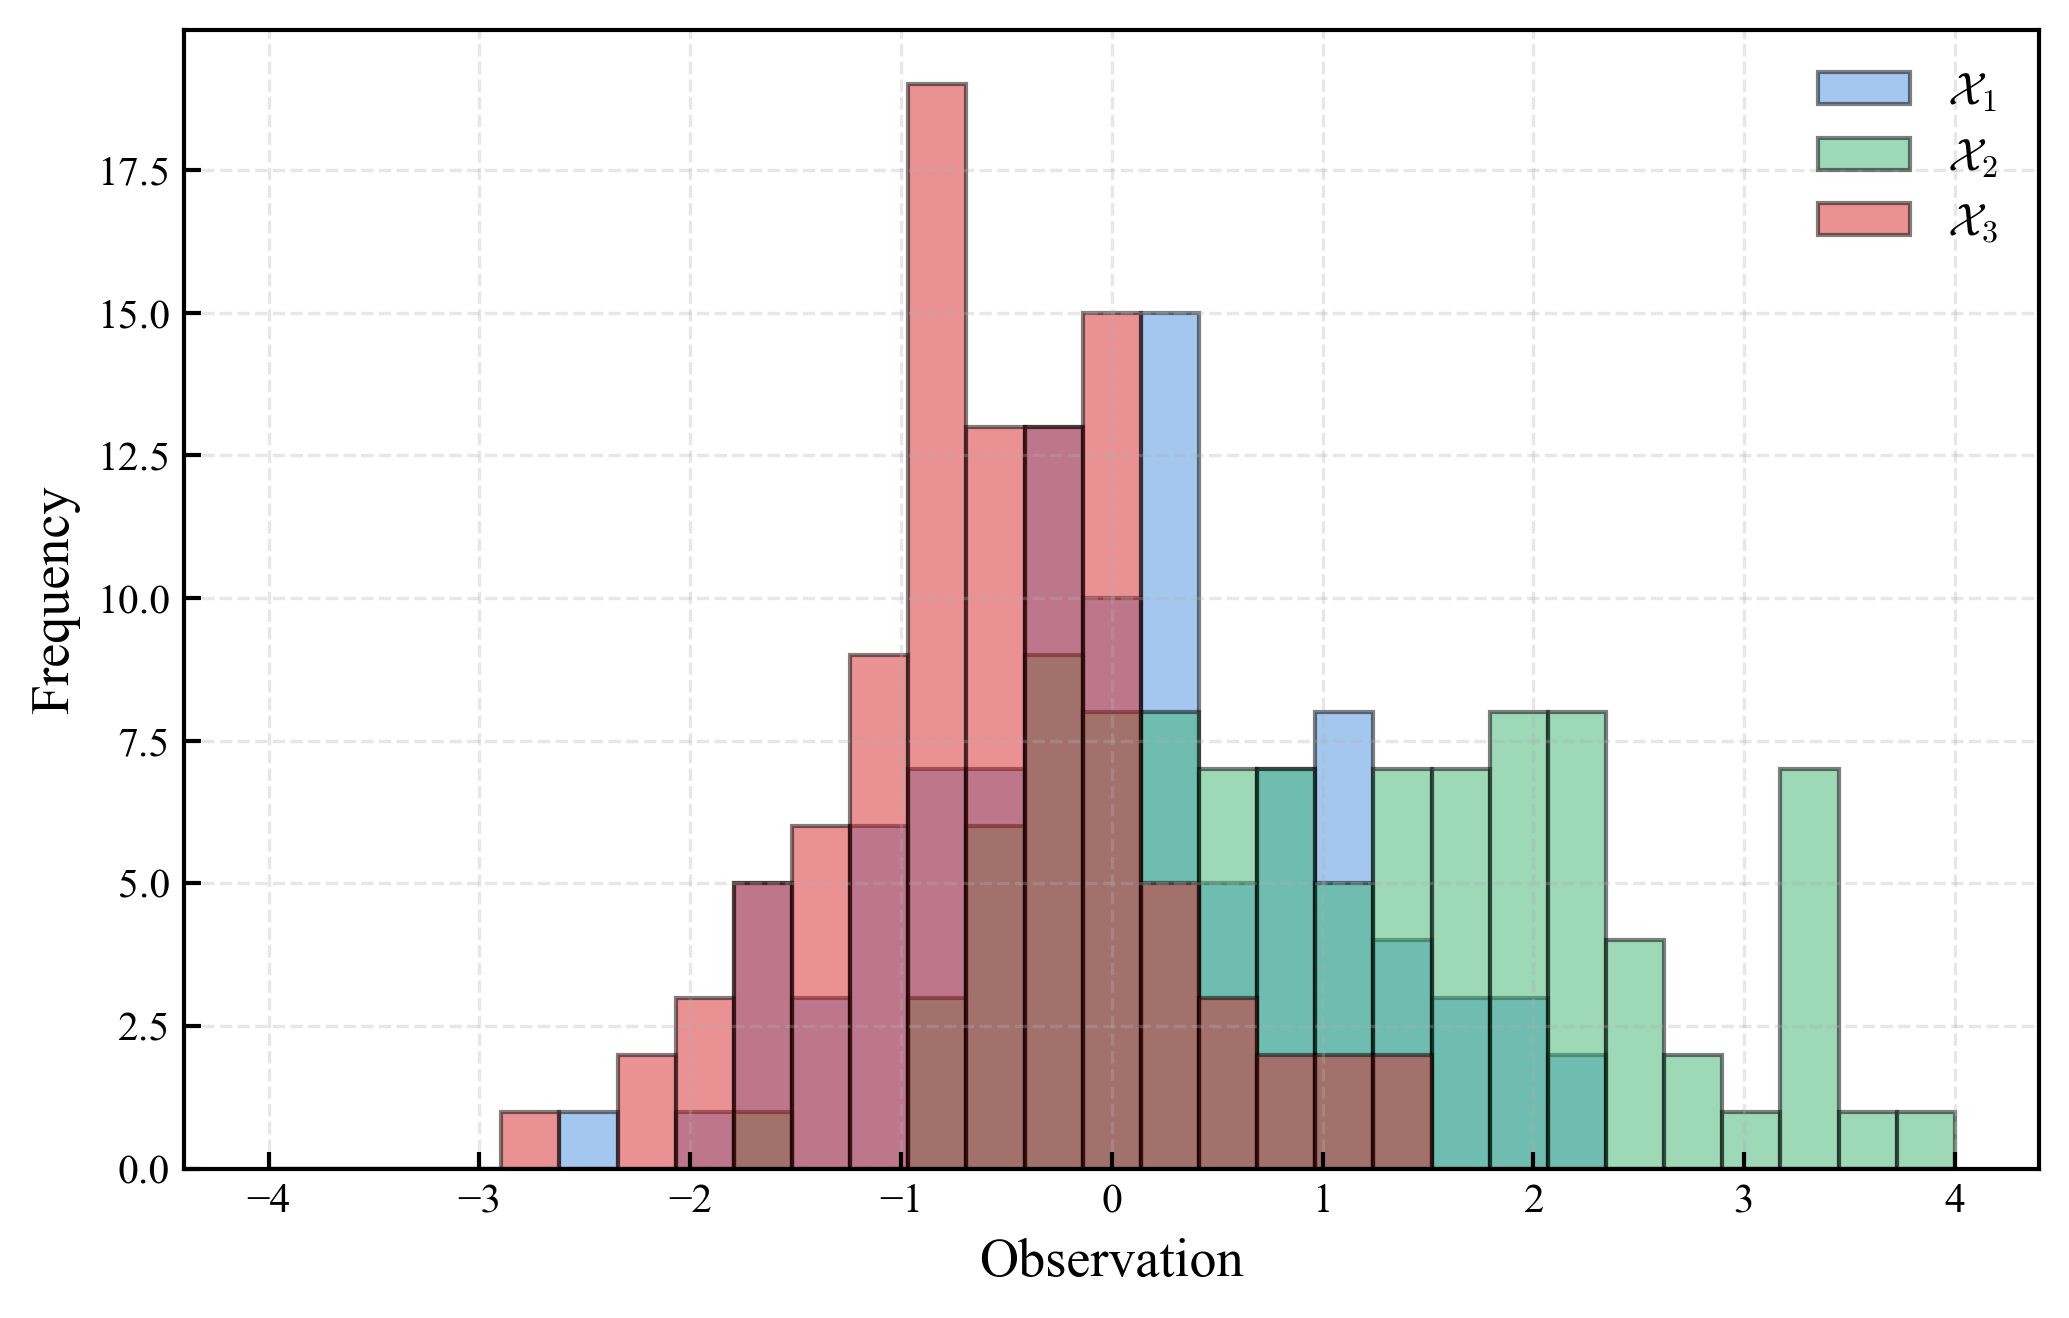
\includegraphics[width=0.6\textwidth]{figures/chapter1/mean_std_hist.png}
    \caption{Three sets of observations, with the mean value and standard deviation represented as a violin plot [...]. The red line shows the mean value, representing the central value where the bulk of events lie, and the shadowed area the standard deviation, as measure of the variability, or how spread the observations are with respect to the mean. In this case the three observation sets, or \textit{samples}, consist of 100 observations. In the case of $\chi_1$, $\chi_2$, $\chi_3$ [...].}
    \label{fig:histogram1}
\end{figure}

\begin{figure}[ht]
    \centering
    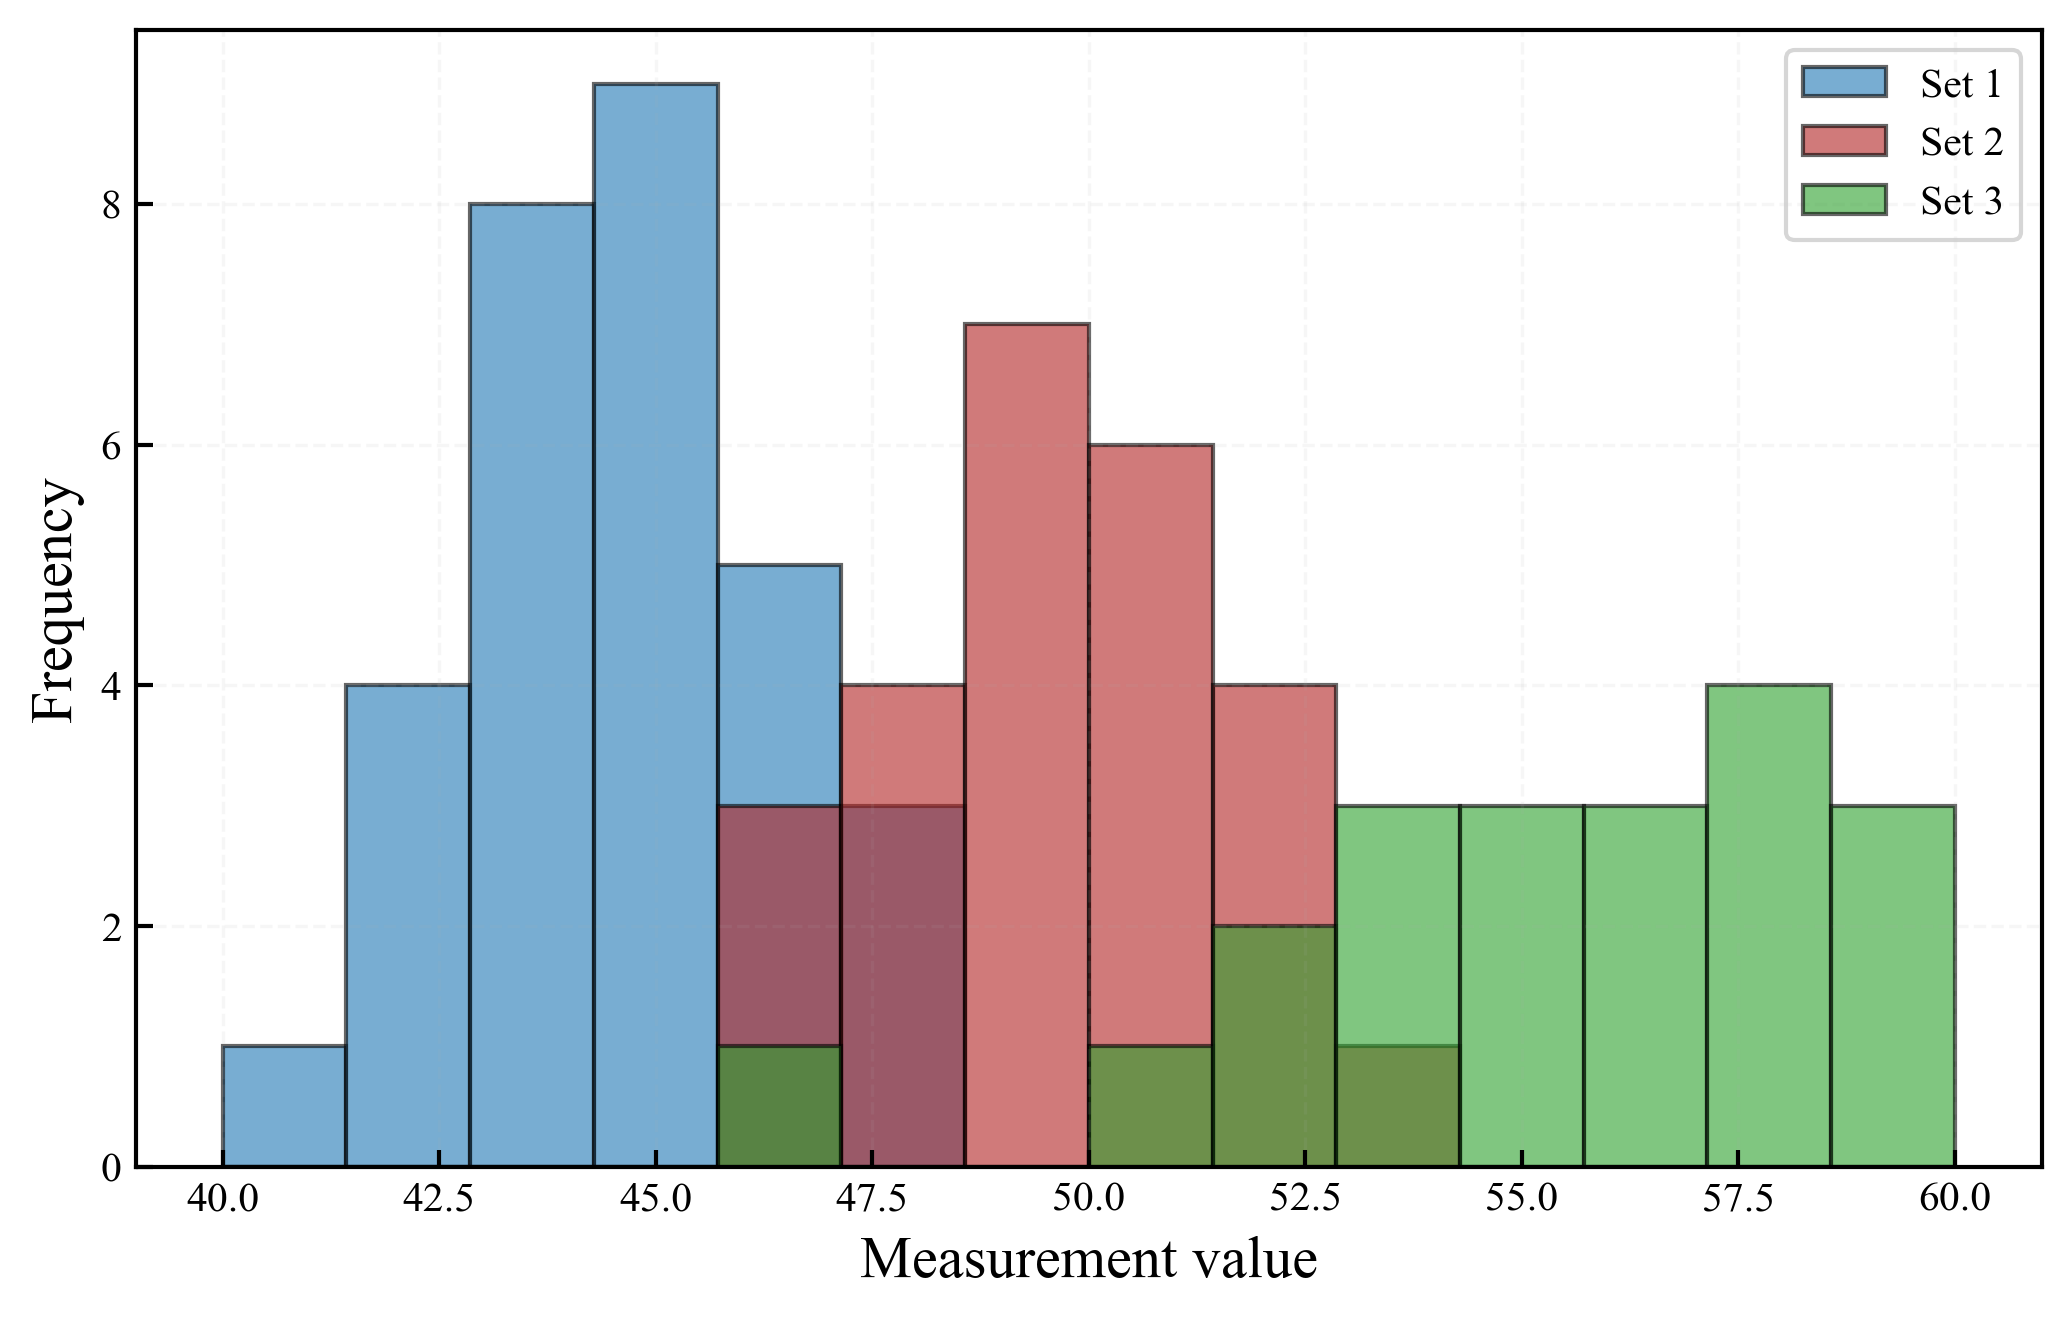
\includegraphics[width=0.6\textwidth]{figures/chapter1/measurements_histogram.png}
    \caption{Three sets of observations, with the mean value and standard deviation represented as a box plot [...]. The red line shows the mean value, representing the central value where the bulk of events lie, and the shadowed area the standard deviation, as measure of the variability, or how spread the observations are with respect to the mean. In this case the three observation sets, or \textit{samples}, consist of 100 observations. In the case of $\chi_1$, $\chi_2$, $\chi_3$ [...].}
    \label{fig:histogram1}
\end{figure}

\section{Data visualization}

\begin{figure}[ht]
    \centering
    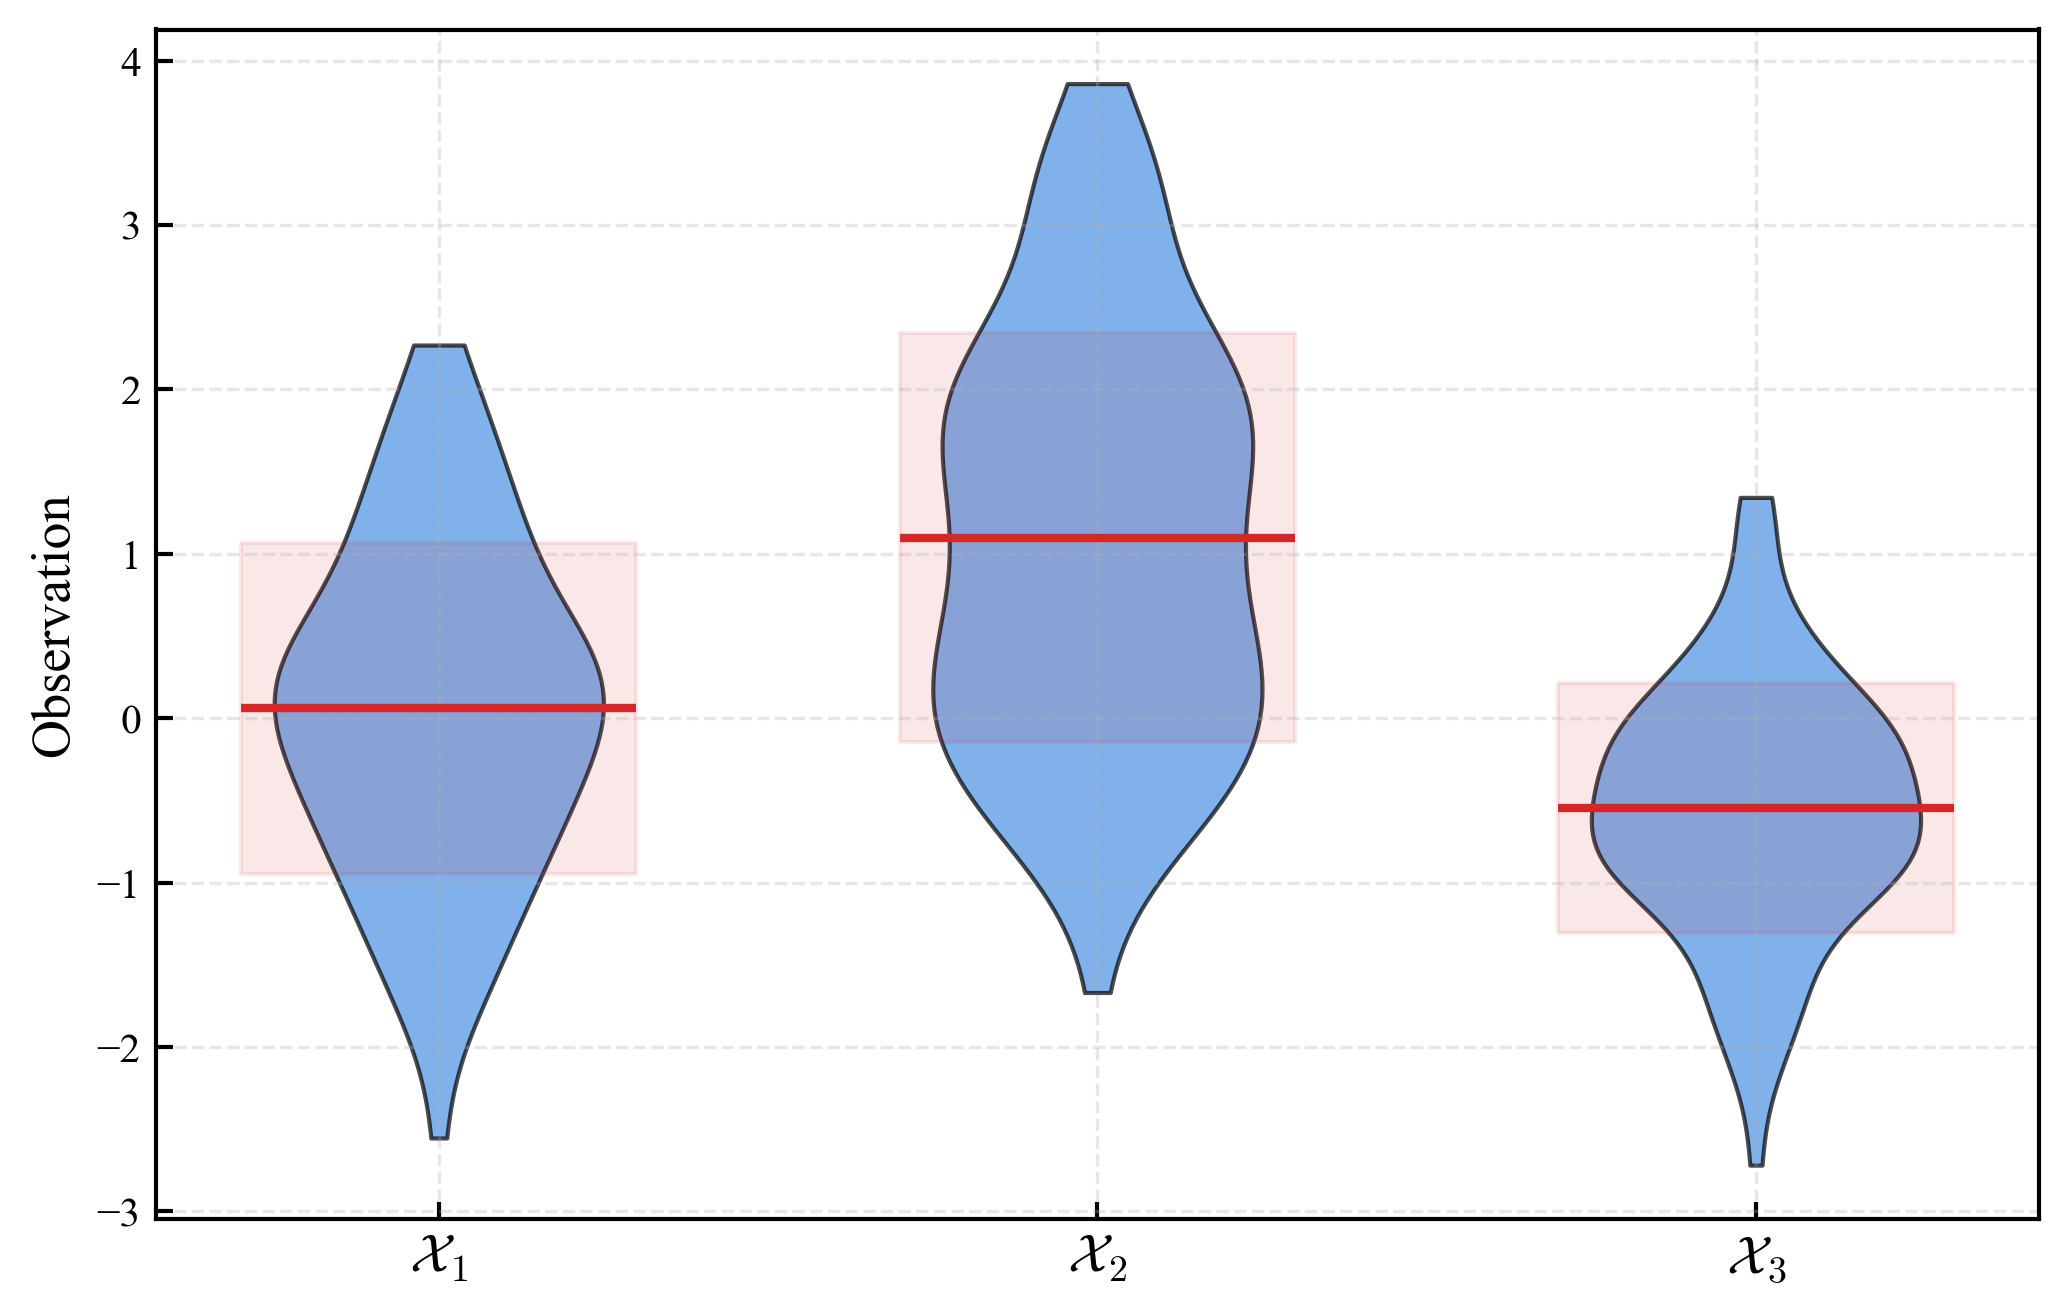
\includegraphics[width=0.6\textwidth]{figures/chapter1/mean_std_violin.png}
    \caption{Three sets of observations, with the mean value and standard deviation represented as a violin plot [...]. The red line shows the mean value, representing the central value where the bulk of events lie, and the shadowed area the standard deviation, as measure of the variability, or how spread the observations are with respect to the mean. In this case the three observation sets, or \textit{samples}, consist of 100 observations. In the case of $\chi_1$, $\chi_2$, $\chi_3$ [...].}
    \label{fig:histogram1}
\end{figure}

\begin{figure}[ht]
    \centering
    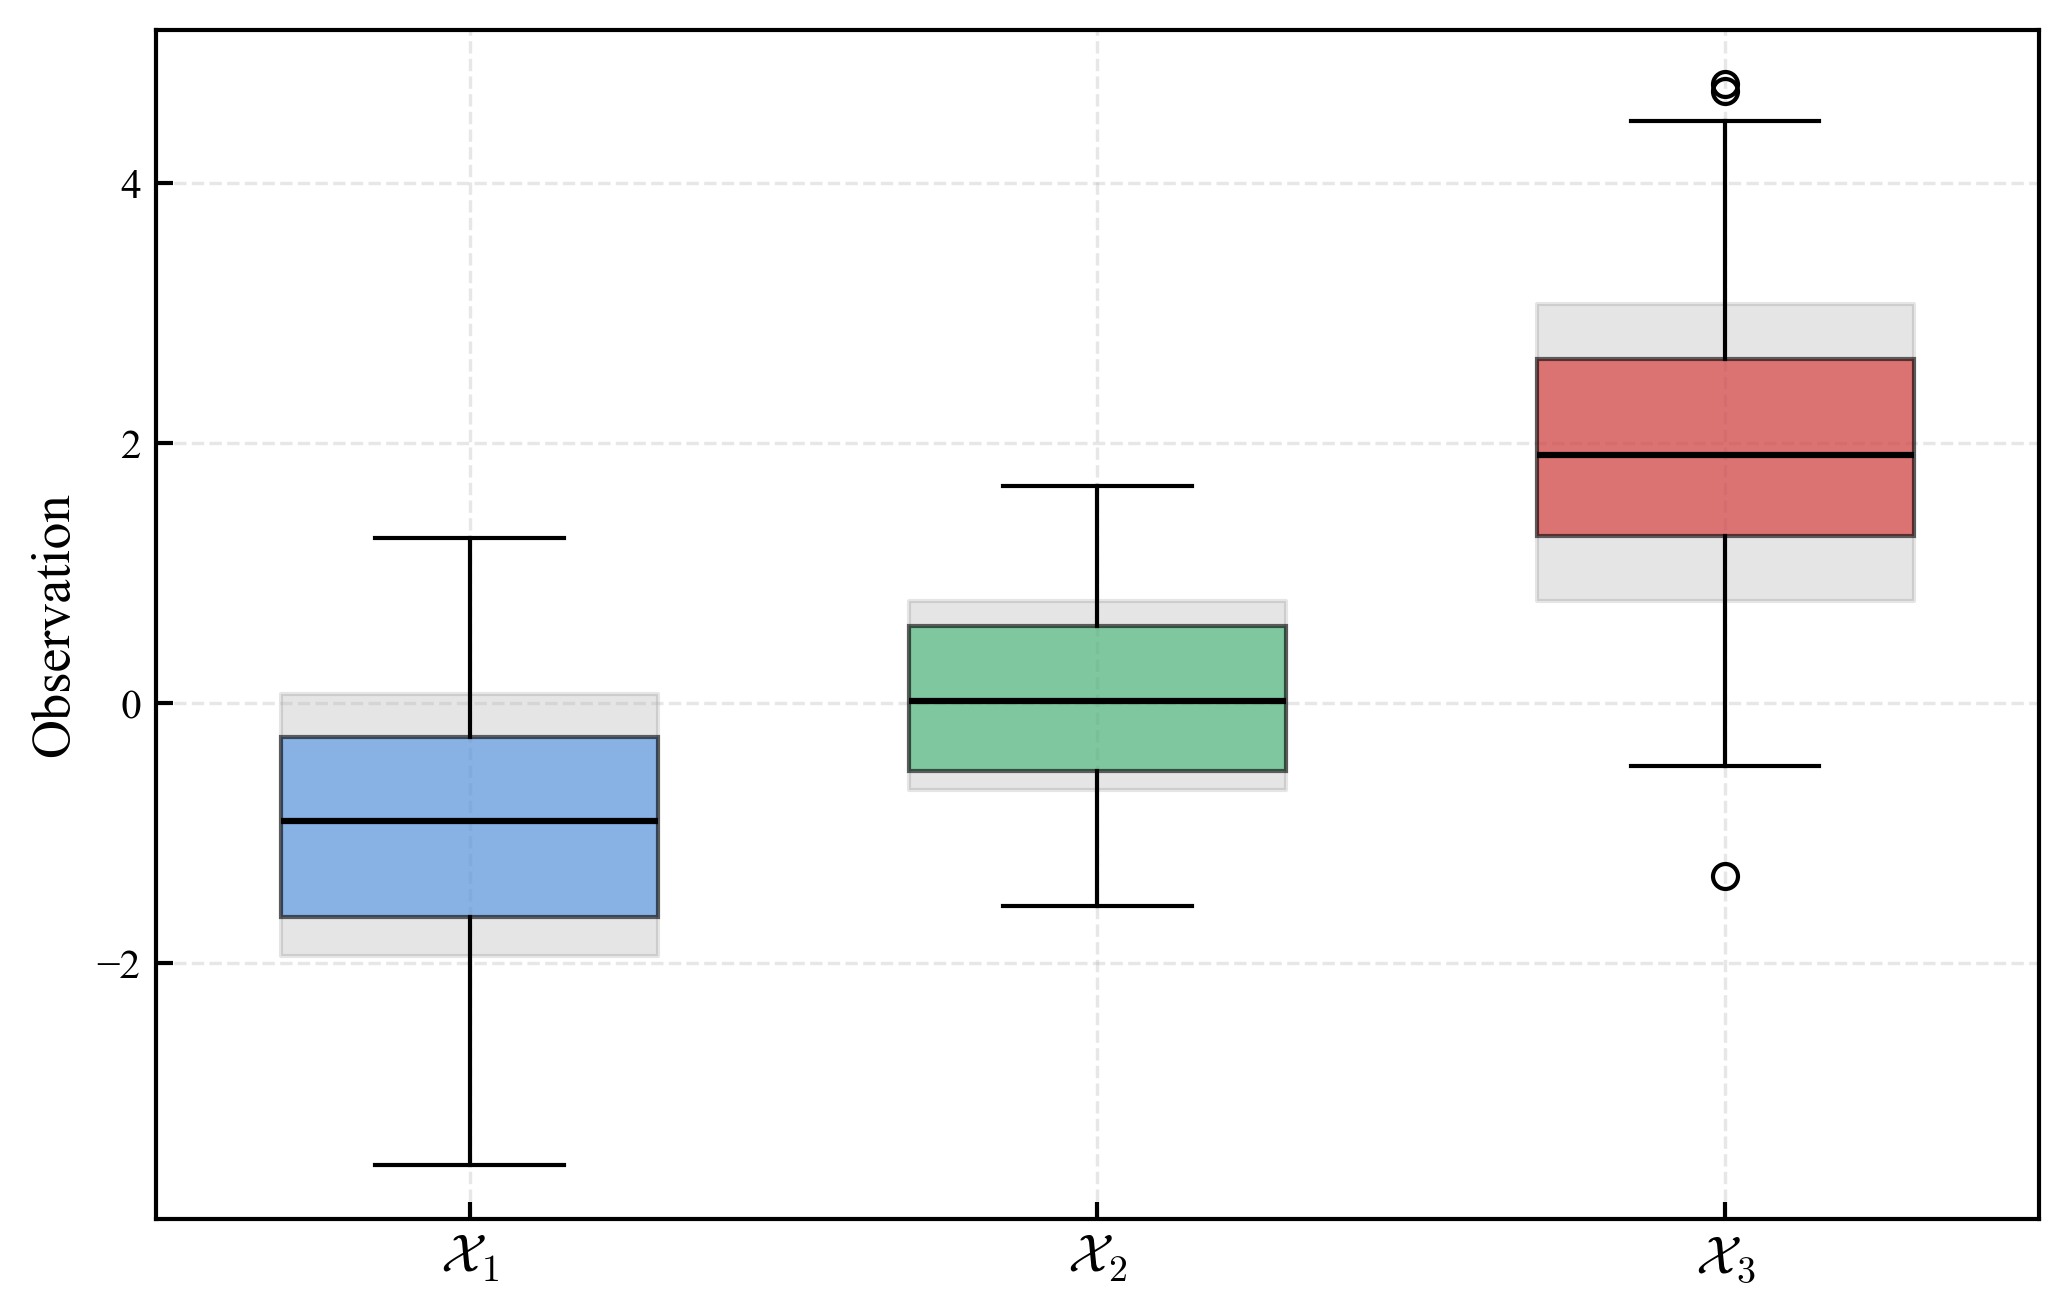
\includegraphics[width=0.6\textwidth]{figures/chapter1/mean_std_box.png}
    \caption{Three sets of observations, with the mean value and standard deviation represented as a box plot [...]. The red line shows the mean value, representing the central value where the bulk of events lie, and the shadowed area the standard deviation, as measure of the variability, or how spread the observations are with respect to the mean. In this case the three observation sets, or \textit{samples}, consist of 100 observations. In the case of $\chi_1$, $\chi_2$, $\chi_3$ [...].}
    \label{fig:histogram1}
\end{figure}

\begin{figure}[ht]
    \centering
    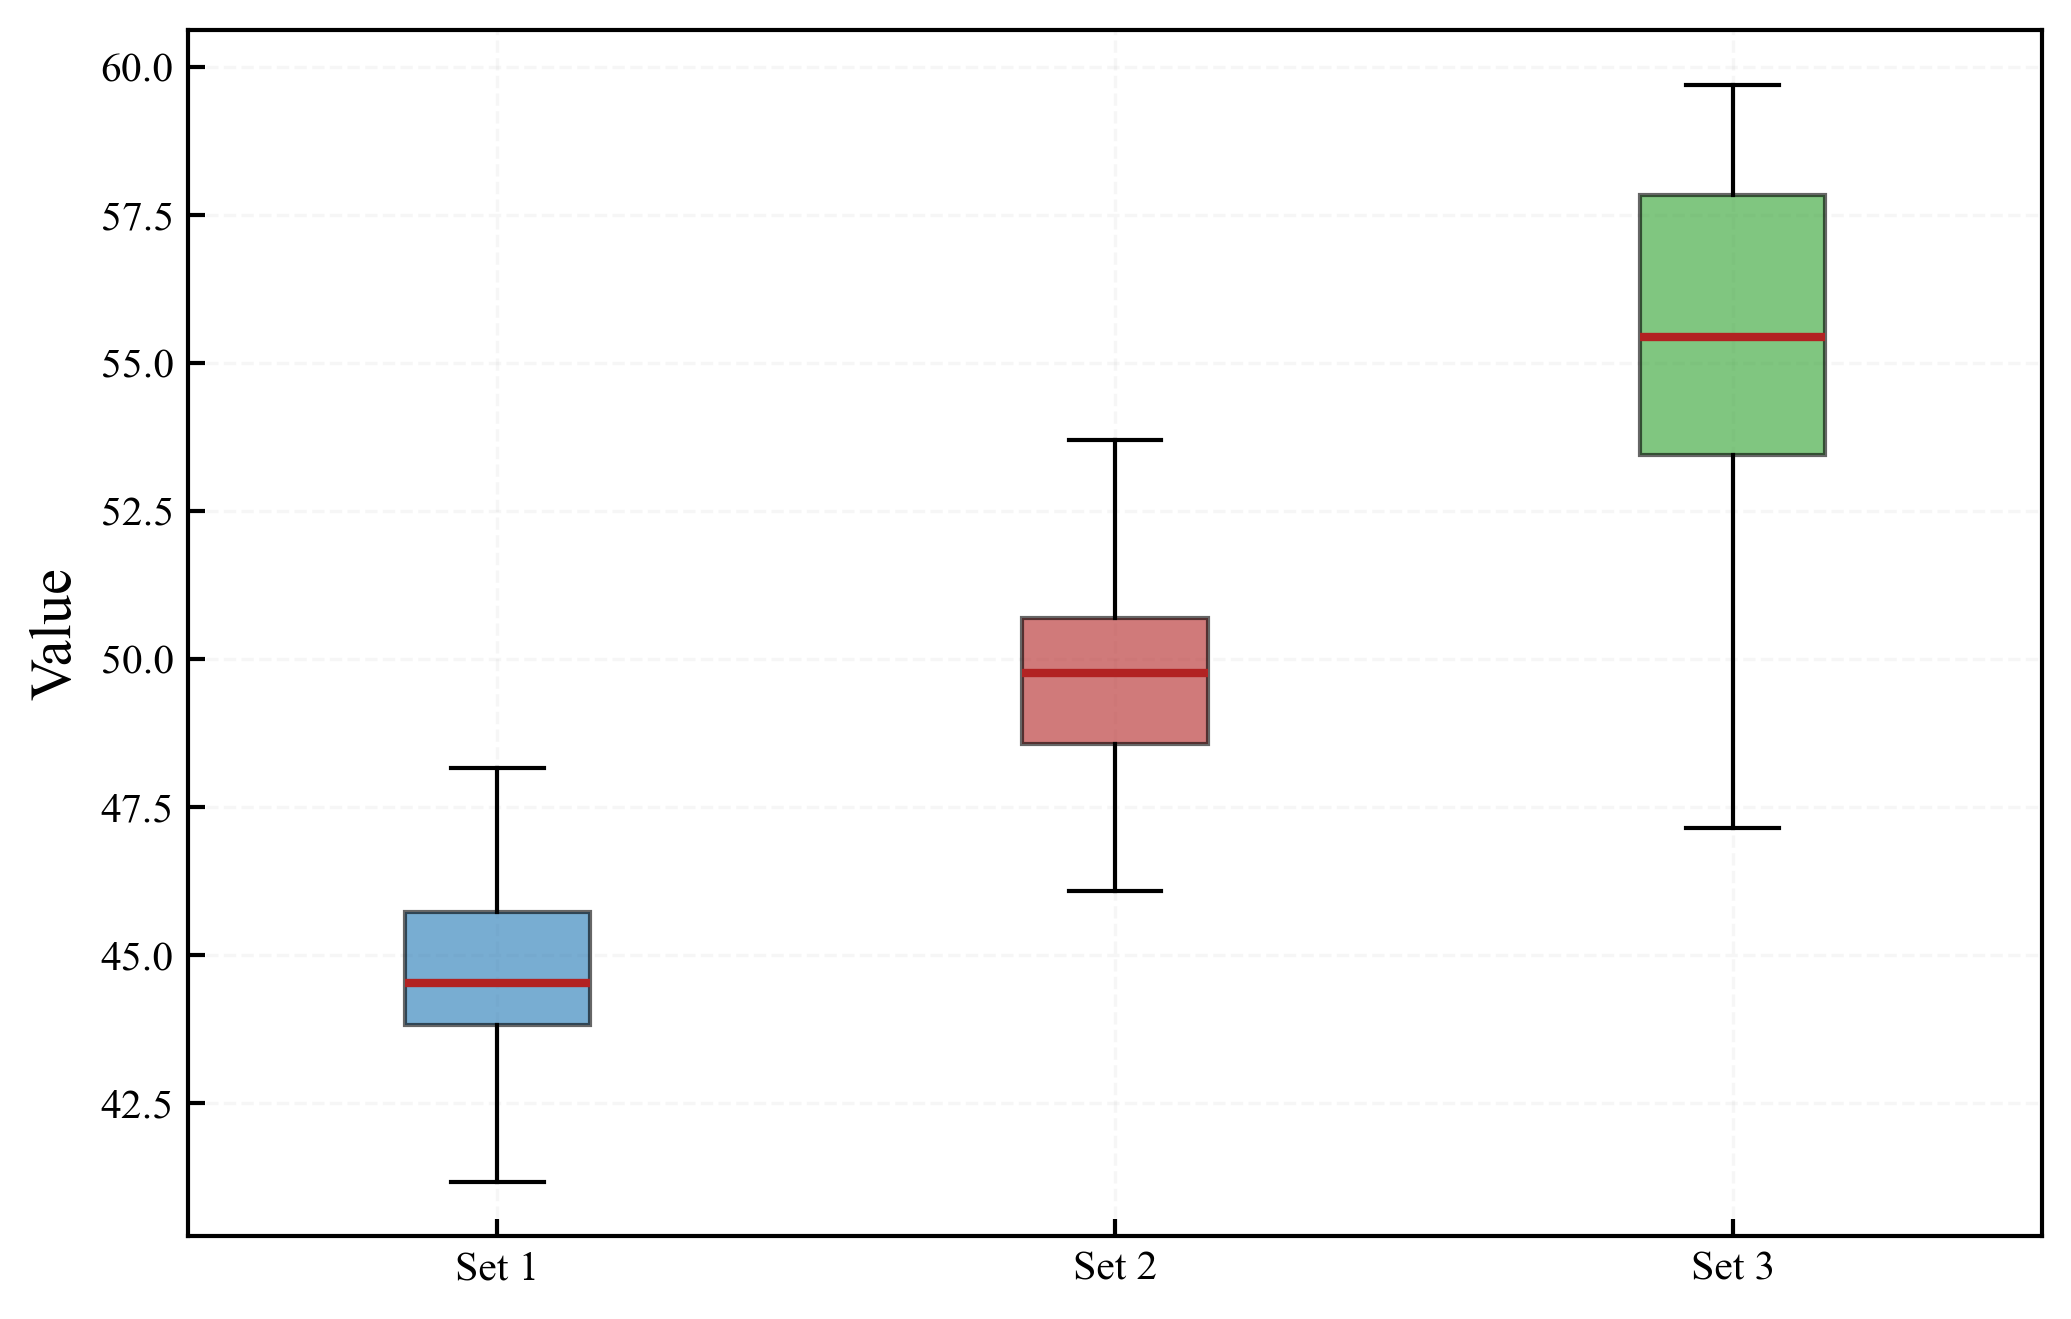
\includegraphics[width=0.6\textwidth]{figures/chapter1/measurements_boxplot.png}
    \caption{Three sets of observations, with the mean value and standard deviation represented as a violin plot [...]. The red line shows the mean value, representing the central value where the bulk of events lie, and the shadowed area the standard deviation, as measure of the variability, or how spread the observations are with respect to the mean. In this case the three observation sets, or \textit{samples}, consist of 100 observations. In the case of $\chi_1$, $\chi_2$, $\chi_3$ [...].}
    \label{fig:histogram1}
\end{figure}

\begin{figure}[ht]
    \centering
    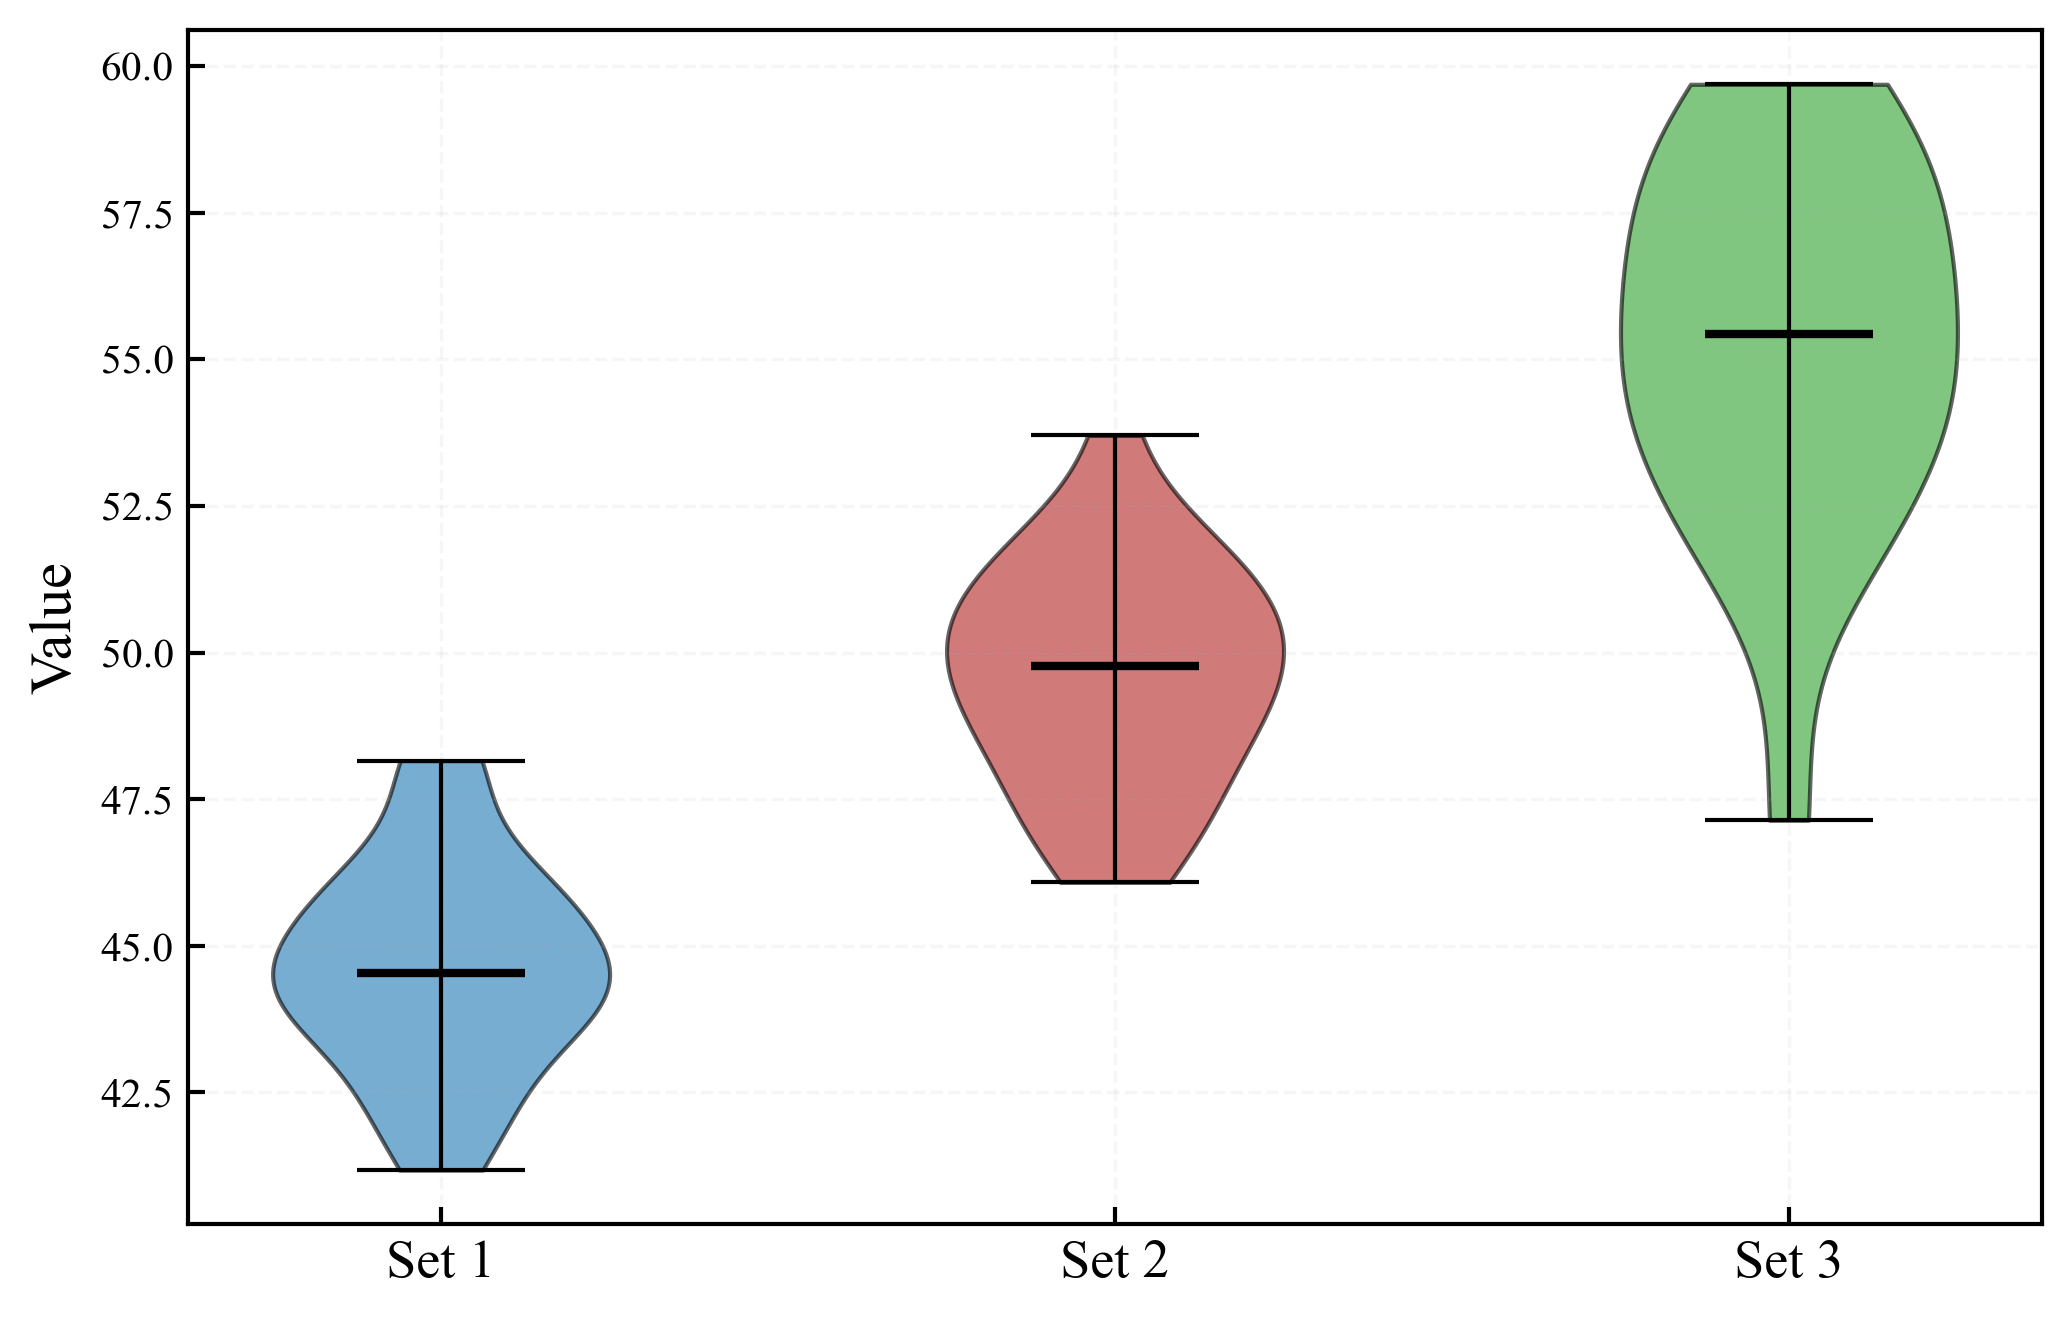
\includegraphics[width=0.6\textwidth]{figures/chapter1/measurements_violin.png}
    \caption{Three sets of observations, with the mean value and standard deviation represented as a box plot [...]. The red line shows the mean value, representing the central value where the bulk of events lie, and the shadowed area the standard deviation, as measure of the variability, or how spread the observations are with respect to the mean. In this case the three observation sets, or \textit{samples}, consist of 100 observations. In the case of $\chi_1$, $\chi_2$, $\chi_3$ [...].}
    \label{fig:histogram1}
\end{figure}

\section{Dependency, linearity, correlation}

Scatter plots: visualize relationships between two quantitative variables.\\

Correlation: introduce Pearson correlation, interpretation, limitations.\\

Optional: mention rank correlation for ordinal data.\\



% Chapter - Probability and random events .........................................................................................................................................................
\chapter{Probability and random events}

\epigraph{\textit{It is through the calculation of probabilities that the divine order becomes visible.}}{— Jacob Bernoulli}

\section{What is probability?}

Probability theory, as we understand it today, did not emerge fully formed from games of chance and repetition. It was gradually sculpted from the abstract yet foundational ideas of \textit{measure theory}, holding the notion that abstract spaces - and randomness too - could be measured. At its core, without getting lost in formalism, we could define probability as a branch of mathematics dealing with information, chance and \textit{random events}. To keep things simple, random events, also referred to as \textit{stochastic}, are simply processes whose output we \textit{ignore}. As classic examples we could think of tossing coins, rolling dice, or performing some arbitrary measurement. Indeed, the word stochastic comes from no other than the greek word \textgreek{στοχαστικός} (stochastic), which literally means \textit{to guess}. Let's try to briefly introduce the idea of probability, as a quantity that describes such events and quantifies our degree of certainty for a specific result.

\medskip

The rigorous formulation begins with the notion of \textit{sample space}, denoted by $\Omega$, introduced in the early 20th century by French mathematician Henri Lebesgue, among others. By \textit{sample space} $\Omega$, we will mean just the set of all possible outcomes of a certain measurement. The other key element is the \textit{measure} $\mu$, introduced in its modern form by Lebesgue in 1902 \cite{lebesgue1902}, and later adapted to probability as $\mathbb{P}$. Together they denoted an abstract mathematical object called the \textit{measure space} $(\Omega, \mu)$, which will eventually become the mathematical language used to described probability. If you want to read more about how measure theory led to probability theory in its its modern form, navigate through the works of Andrey Kolmogorov, specially his 1933 monograph \textit{"Foundations of Theory of Probability} \cite{kolmogorov1933}, where he formalized probability spaces using measure-theoretic language.

\medskip

Let's ask ourselves a the question, what \textit{is} probability in the first place? What do we mean by it and what does it describe? Probability is nothing more, and nothing less, that a \textit{number} we make up, a \textit{quantity} we come up with, to quantify certainty in a process whose outcome we ignore. A number we will use to describe the amount of information we have about a random - or stochastic - event. For simplicity, we can make it range from 0 to 1, in the following way:

\begin{itemize}
\item If I'm sure that some event (A) will never happen, $P(A) = 0$.
\item If I'm sure that some event (A) will always happen,  $P(A) = 1$.
\item For anything in between, if I'm not certain about any of the outcomes, $P(A) \in [0, 1]$.
\end{itemize}

With the symbol $ \in$ we simply denote that $P(A)$ will be a number between 0 and 1. It could also be read as $P(A)$ is \textit{contained} in the interval $[0, 1]$. In all those cases where we are not sure if we will get one result or another, we say that there is a level of \textit{uncertainty}, or \textit{surprise} [...].\\

Let's think on a coins toss, as an example. To model such case, one of the simplest and oldest examples of a stochastic process, we would have two possible outcomes: heads ($H$), and tails ($T$).

\begin{itemize}
\item If I'm sure I will get heads, $P(H) = 1$, and $P(T) = 0$.
\item If I'm sure I will get tails, $P(H) = 0$, and $P(T) = 1$.
\item For anything in between, $P(H) = P(T) = \frac{1}{2}$.
\end{itemize}

The scenarios in which I am certain, of either one case of the other, are clear. But for the third one, where we assign a value to the probability which is not 0 or 1, we should stop for a second. When we say that the probability of getting heads - or tails - in a normal coin that is not biased is $P = \frac{1}{2}$, we are implicitly assuming some things. We implicitly assume that if we repeated the toss many times, half of them we would get one result (e.g., heads), and the other half the remaining result (e.g., tails). This is normally referred to as the \textit{frequentist} definition of probability, because we are defining its value as the ratio of how many times we get a specific result $n$, and the number of total trials $N$. The example of the coin, where we have just two possible results, is what we will call a \textit{Bernoulli} trial, and we will describe it in detail soon, but let's use it now as a prior example to introduce the idea of probability [...] .\\

\begin{equation}
	P(\text{A happening}) = \frac{\text{Number of times A happens}}{\text{Total number of trials}} = \frac{n}{N} \; . \nonumber
\end{equation}

In the case of the coin, if I toss 100 times, and obtain 55 heads against 45 tails, would lead to 

\begin{equation}
	P(\text{H}) = \frac{55}{100} \simeq \frac{1}{2} \; . \nonumber
\end{equation}

Ideally we expect that these frequencies, as we increase the number of repetitions, would approach a perfect $\frac{1}{2}$. We will revisit this concept when we talk about the Law of Large Number and the Central Limit Theorem, in Chapter 3.\\

But this is not the only thing we assume about such a quantity. For probabilities to represent the real behaviour of random processes and information, they must follow another property, called \textit{unitarity}. Unitarity ensures that, if we consider and add up the probabilities for all possible events in a given experiment, we recover the total. That means, at least one of the scenarios will happen.\\

The formal definition of unitarity can be written as follows. Let's denote all possible outcomes of an experiment $x_{1}$, $x_{2}$, ..., $x_{n}$. In the case of coins these will be just $x_{1} = H$, $x_{2} = T$, and with dice, $x_{1} = 1$, $x_{2} = 2$, ..., $x_{6} = 6$. By \textit{unitarity}, we mean that the sum of probabilities of all possible outcomes \text{add up to 1}. 
\begin{equation}
	\sum_{i = 1}^{n} \; P(x_{i}) = 1
\end{equation}

To transition from \textit{measure} to \textit{probability} theory, Kolmogorov imposed a single but profound condition: the total \textit{measure} $\mu$ of the entire \textit{space} $\Omega$ must equal 1. In modern language, we would call this \textit{normalization}, or \textit{unitarity}. This reflects the fact that, when performing a measurement or an observation - for instance, we are tossing a coin, our sample space would be either heads (H) and tails (T) $\Omega = [H, T]$ The we know - empirically - and we impose - mathematically, that regardless of the probabilities for H and T - same in a normal, fair coin, uneven in a biased one, the probabilities need to sum one, ensuring that either H or T is going to happen. This normalization - declaring that \textit{something must happen} - turns the measure space into a probability space \((\Omega, \mathcal{F}, \mathbb{P})\), and laid the axiomatic foundations for all of modern probability \cite{kolmogorov1933}.

\begin{equation}
	\mathbb{P} (\Omega) = 1
\end{equation}

Means that the sum of probabilities for the case \textit{heads} H and \textit{tails} T must be 1. 

\medskip

From this foundation emerged the full architecture of probability theory. \emph{Random variables} as measurable functions, further refined through the work of Wiener and Doob in the context of stochastic processes \cite{doob1953}. \emph{Expectation} defined via the Lebesgue integral, again rooted in Lebesgue’s work on integration \cite{lebesgue1902}. \emph{Convergence theorems}, including the strong and weak laws of large numbers, were developed through the efforts of Borel (1909), Cantelli (1917), and Kolmogorov (1930s) \cite{billingsley1995}.

\medskip

Yet mathematics alone does not yield interpretation. Here, philosophy enters. The \emph{frequentist} interpretation was developed during the late 19th and early 20th centuries, most notably by Richard von Mises, who defined probability as the limit of relative frequencies in a long sequence of trials \cite{vonmises1928}. In this view, probability is an objective property of the physical world, accessible through repetition. In contrast, the \emph{Bayesian} perspective has older roots. Thomas Bayes introduced the foundational theorem in the 18th century \cite{bayes1763}, but it was Pierre-Simon Laplace who first framed probability as a logic of belief and inference \cite{laplace1812}. The modern subjective Bayesian school was revived in the 20th century by Bruno de Finetti, who emphasized coherence and personal belief as central principles \cite{definetti1974}.

\medskip

These two interpretations - frequentist and Bayesian - do not so much contradict as illuminate different dimensions. The frequentist roots itself in empirical regularity, the Bayesian in epistemic uncertainty. Both, however, rest on the same mathematical foundation: a probability is a measure, and measures give form to uncertainty. 

\medskip

Indeed, the literal meaning of probability comes from latin \textit{probabilis}. American logician and philosopher Richard Jeffrey, "Before the middle of the seventeenth century, the term "probable" (Latin probabilis) meant just approvable, and was applied in that sense, univocally, to opinion and to action. A probable action or opinion was one such as sensible people would undertake or hold, in the circumstances." However, in legal contexts especially, "probable" could also apply to propositions for which there was good evidence [...].

\medskip

There have been at least two successful attempts to formalize probability, namely the Kolmogorov formulation and the Cox formulation. In Kolmogorov's formulation (see also probability space), sets are interpreted as events and probability as a measure on a class of sets. In Cox's theorem, probability is taken as a primitive (i.e., not further analyzed), and the emphasis is on constructing a consistent assignment of probability values to propositions. In both cases, the laws of probability are the same, except for technical details [...].\\

\section{Discrete random variables}

So far we have introduced the idea of random events, and the concept of probability as a number we define to quantify uncertainty. Now, we will try to model such events aiming to build predictions. That way, the probability we just defined will become a \textit{function} of certain input information, to be a descriptive - or \textit{predictive} - quantity. Indeed, not all random events are equal, and we will use the \textit{distribution} of such probabilities to classify different families of stochastic events.
  
 \subsection{Bernoulli distribution}

The simplest case we can think of is the \textbf{Bernoulli event}, or \textit{Bernoulli trial}, named after Swiss mathematician Jacob Bernoulli in late 1600s. A Bernoulli trial is a random experiment with exactly two possible outcomes: either \textit{success}, usually labeled as 1, and \textit{failure}, labeled as 0. Tossing a coin - aiming for \textit{heads} as success and \textit{tails} as failure - or rolling dice aiming for any particular face, are typical examples of Bernoulli trials. The probability of success ($1/2$ in the case of a fair coin, $1/6$ for any of the faces of the dice, is normally denoted by $p$. Since we only care about that particular case, the probability of failure is the remaining one, $1 - p$.\\

Mathematically, we write a Bernoulli trial on random variable $x$ as follows:
\begin{equation}
	P(\text{success, when} x = 1) = p \quad \text{and} \quad P(\text{failure, when} x = 0) = 1 - p \; .
	\label{eq:bernoulli}
\end{equation}

In the case of tossing a coin, the random variable $x$ will be just the face, either \textit{heads} ($x = 1$), with probability $p = 1/2$ or \textit{tails} ($x = 0$), with probability $p = 1/2$ and we would write it in the following way:
\begin{equation}
	P(x = 1; \text{heads}) = \frac{1}{2} \quad \text{and} \quad P(x = 0; \text{tails}) = \frac{1}{2} \; .
	\label{eq:bernoulli_1}
\end{equation}

In the case of rolling a dice and aiming for, let's say, a 6 - or any other value - the random variable $x$ will be again the face, now either a successful 6 ($x = 1$), with probability $p = 1/6$ or any other result as failure ($x = 0$), with probability $p = 5/6$
\begin{equation}
	P(x = 1; \text{face = 6}) = \frac{1}{6} \quad \text{and} \quad P(x = 0; \text{face $\neq$ 6}) = \frac{5}{6} \; .
	\label{eq:bernoulli_2}
\end{equation}

Note that in all cases, the probability $p$ remains a number between 0 and 1, consistent with our definition $p \in [0, 1]$ on previous section. Note as well that probabilities of both cases, success and failure, always add up to 1, conveniently fulfilling the unitarity property in the case of $n = 2$ possibilities.
\begin{equation}
	\sum_{i = 1}^{n} \; P(x_{i}) = P(x_1) + P(x_2) = p + (1 - p) = 1 \; .
\end{equation}

From now on, rather than just writing the probabilities, we will build a quantity called \textit{distribution}. This may sound a bit abstract at first, but it will prove extremely useful when dealing. Indeed, even familiar quantities like the mean or the variance can be defined mathematically in terms of \textit{expected values}, or \textit{momenta} of probability distributions, as we will see further in this chapter.\\

The way we will write Bernoulli trials \eqref{eq:bernoulli} as a \textit{probability distribution} is 
\begin{equation}
	P(x; p) = 
		\begin{cases}
			p & \text{if $x = 1$, success} \\
			1 - p & \text{if $x = 0$, failure}
		\end{cases}
\end{equation}

Note that now, the probability distribution, written with upper case $P$, is a function of two input quantities, the random variable $x$, that can take two values (1 for success, 0 for failure) \textit{and} the probability for each case, $p$ when success and $(1 - p)$ when failure.

In the case of tossing a coin, the distribution for Bernoulli trial  \eqref{eq:bernoulli_1} will become just 
\begin{equation}
	P(x; p) = 
		\begin{cases}
			\frac{1}{2} & \text{if $x = 1$, heads} \\
			\frac{1}{2}& \text{if $x = 0$, tails}
		\end{cases}
\end{equation}

\begin{figure}[ht]
    \centering
    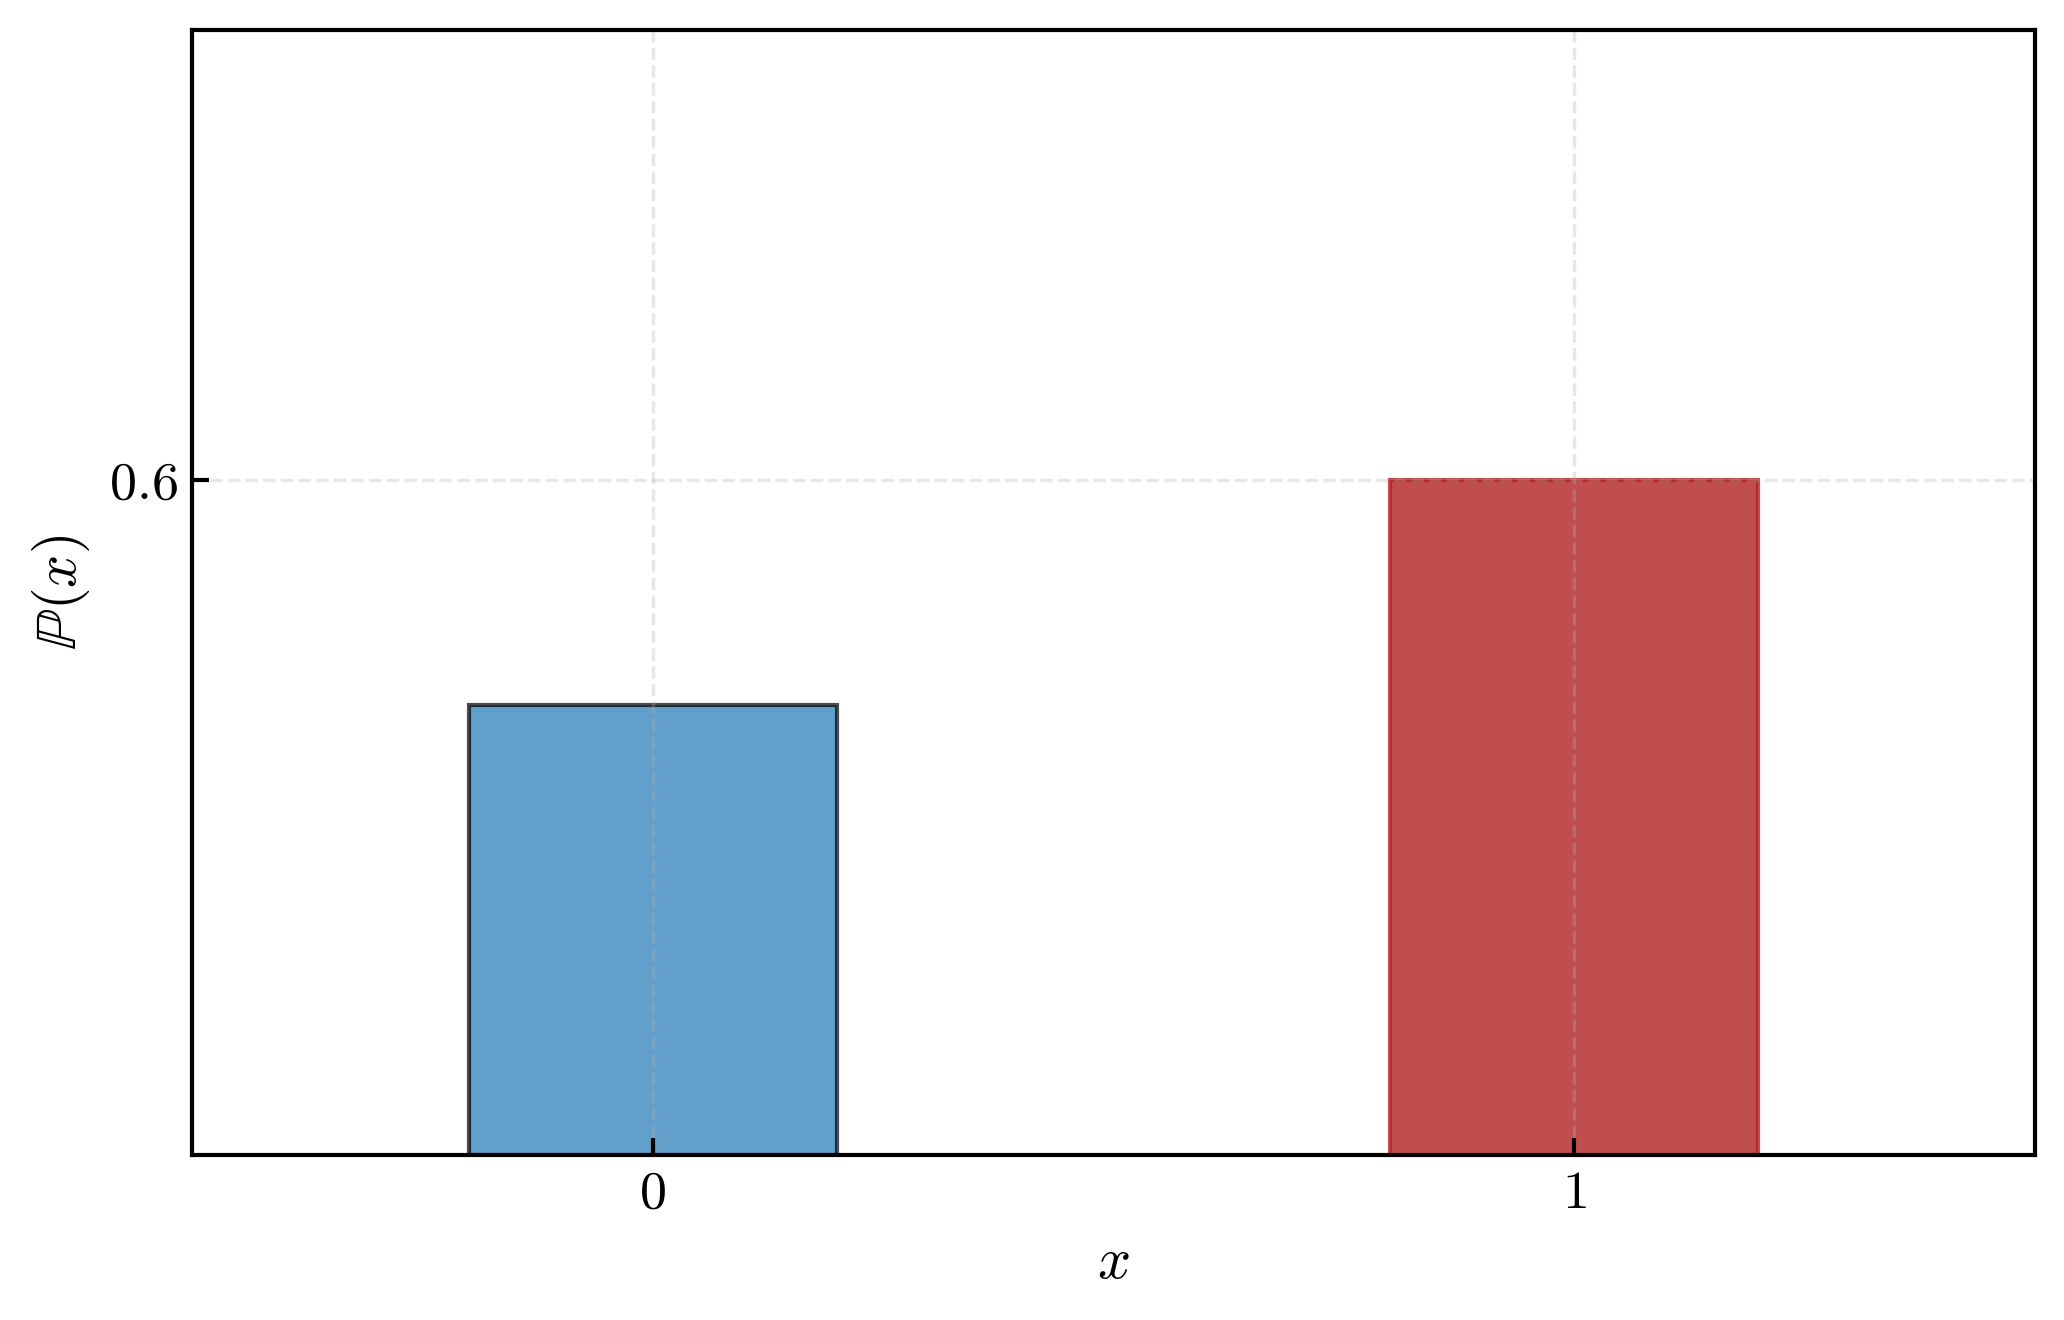
\includegraphics[width=0.7\textwidth]{figures/chapter2/bernoulli_1.png}
    \caption{Representation of the Bernoulli distribution for a coin toss. The random variable $x$ represents the face of the coin measured after the toss, either heads ($x = 1$) or tails ($x = 0$), each with equal probability of happening $p = 1/2$.}
    \label{fig:bernoulli_1}
\end{figure}

In the case of rolling, the distribution for Bernoulli trial  \eqref{eq:bernoulli_2} will become just 
\begin{equation}
	P(x; p) = 
		\begin{cases}
			\frac{1}{6} & \text{if $x = 1$, face we want} \\
			\frac{5}{6}& \text{if $x = 0$, any other value}
		\end{cases}
\end{equation}

\begin{figure}[ht]
    \centering
    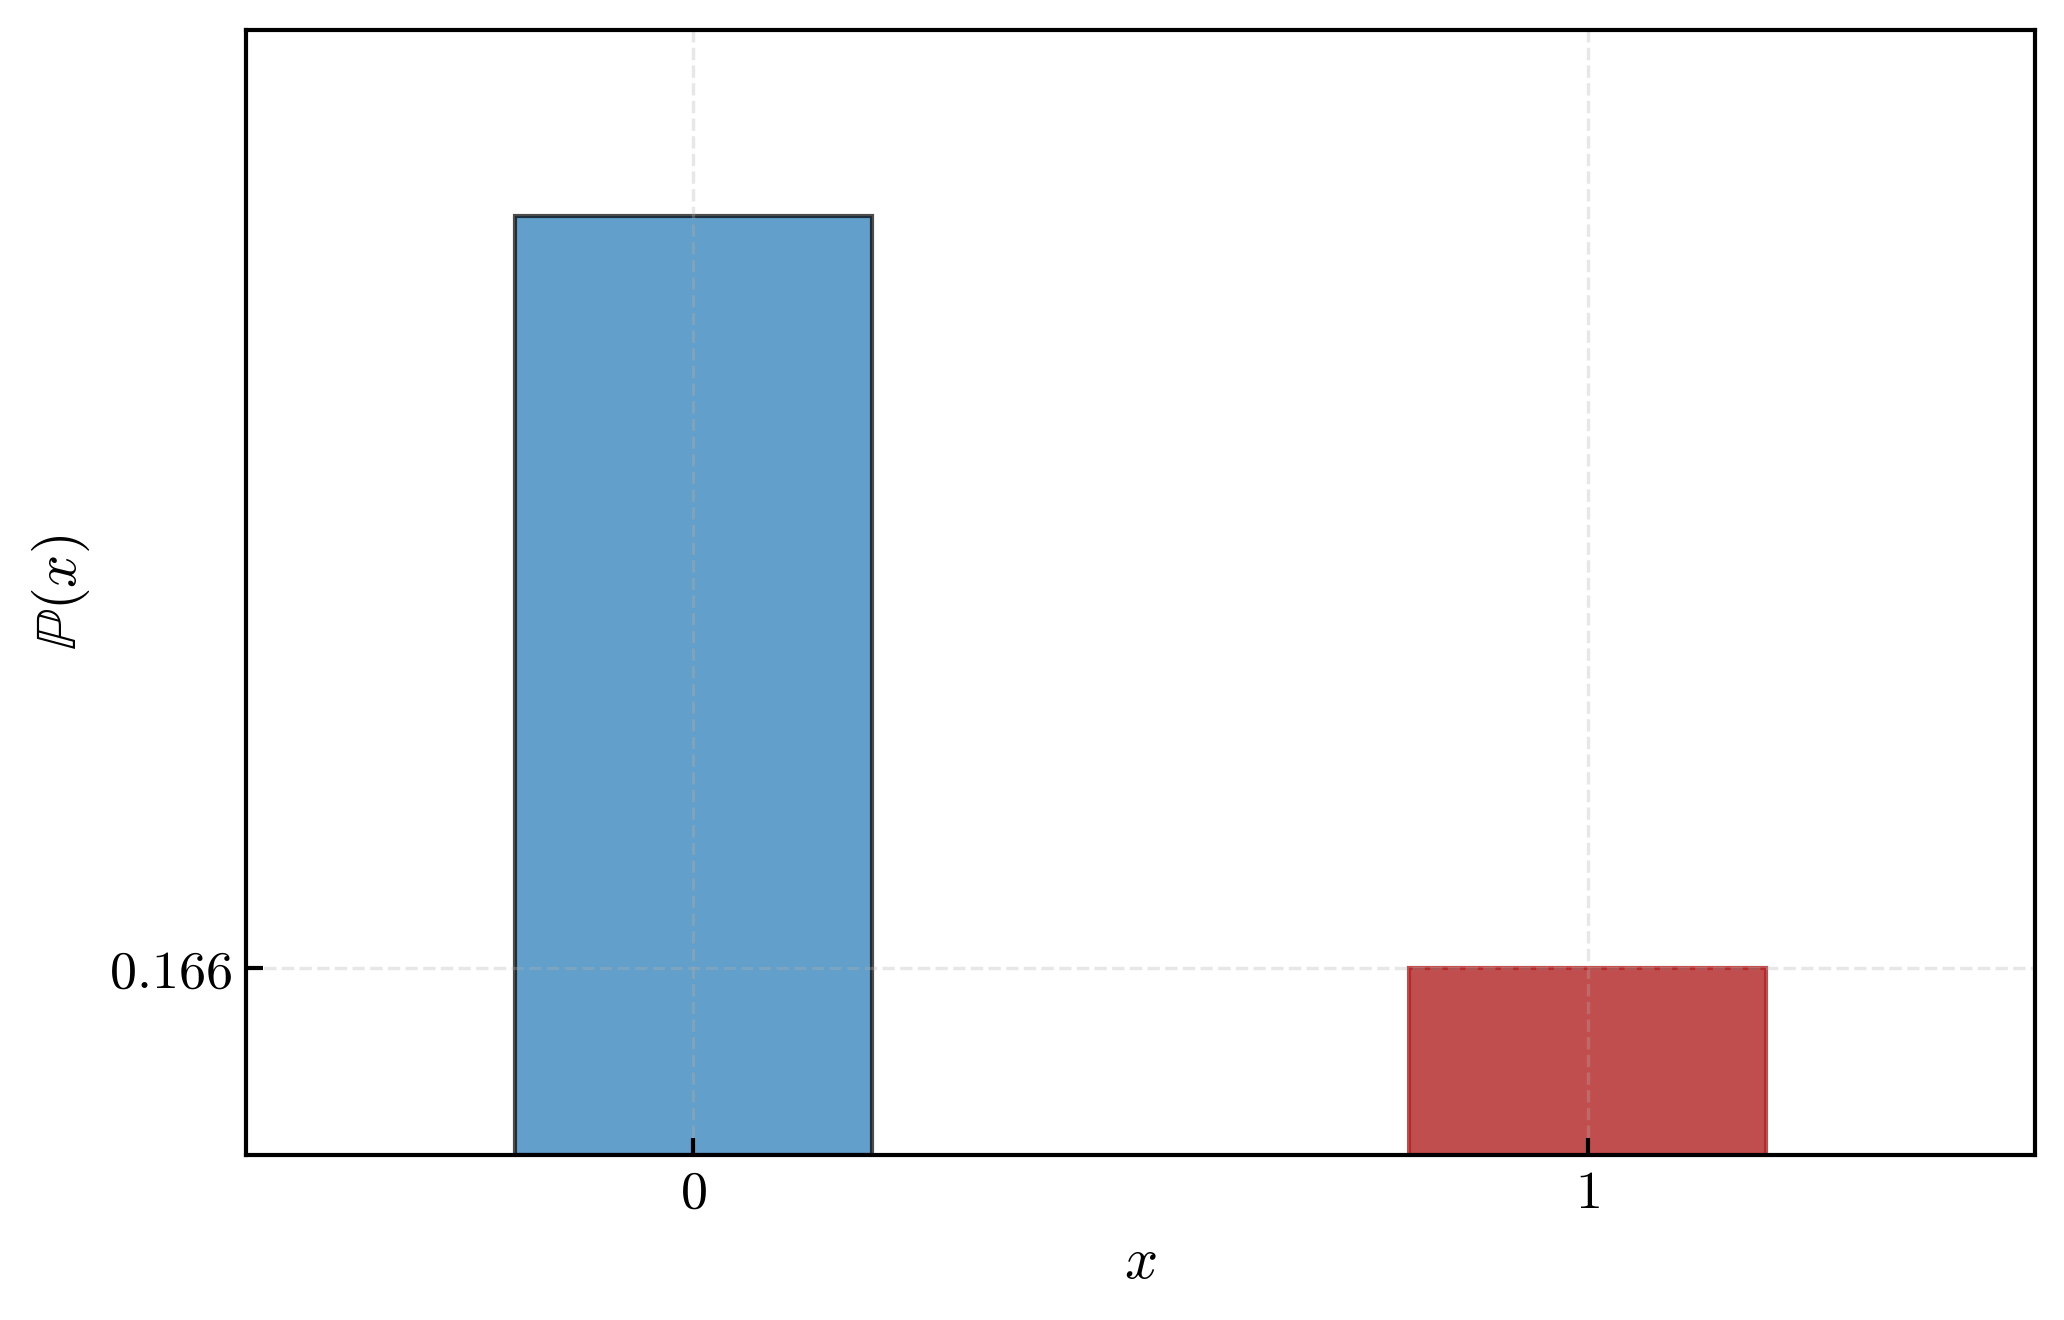
\includegraphics[width=0.7\textwidth]{figures/chapter2/bernoulli_2.png}
    \caption{Representation of the Bernoulli distribution for a dice roll. The random variable $x$ represents the face of the dice measured after the roll, either a 6 - or any other face in a fair dice - ($x = 1$) or any of the remaining values, labeled as failure ($x = 0$). The probability of obtaining any of the faces is now $p = 1/6$, and any of the remaining ones appear with $1 - p = 5/6$.}
    \label{fig:bernoulli_2}
\end{figure}

Jacob Bernoulli stands among the foremost pioneers of probability theory. His work \textit{Ars Conjectandi}, published posthumously in 1713, provided the first systematic framework for reasoning about chance and uncertainty, as we have just seen. As we will cover in further chapters, Bernoulli articulated the law of large numbers, demonstrating that the relative frequency of an event approaches its true probability as the number of trials increases.\\

As one could expect, this did not happen in isolation. The intellectual roots of Bernoulli’s work can be traced some decades earlier to the mid-seventeenth century, when Blaise Pascal and Pierre de Fermat corresponded on problems of games of chance [...]. Their exchange laid the early foundations of combinatorial probability, which Christiaan Huygens and later the Bernoulli family would extend with increasing rigour.\\

It was within this tradition, that Jacob Bernoulli formalized the concept of what we now call a Bernoulli trial we have just covered. A simple experiment yielding one of two outcomes, often described as “success” or “failure”. This notion is elegantly expressed in its most elementary form \eqref{eq:bernoulli}, which captures the dual nature of uncertainty at the heart of probability. From this simple yet deep structure emerges the \textbf{Binomial distribution}, which we will cover next. A model that captures the number of successes in a \textit{sequence} of independent trials.

\subsection{Binomial distribution}

Once we understand Bernoulli trials, and we are familiar with the idea of probability distribution, we can start looking at series of trials, rather than individual random events. We will now make a certain number of measurements $n$, each of them with two or more possible outcomes, and we will try to model the probability of obtaining some - let's call it now $x$ successful results. The question we are after is, what is the probability of observing $x$ positive results, out of $n$ total trials, where the probability of success each time is given by some probability $p$.\\

Back to our routine examples, what will be the probability of obtaining 5 heads if I toss 10 coins? Or what would be the probability of obtaining 5 times a 6, out of a total of 10 dice rolls? In all these cases we will call $x$ the number of successes we want to observe, $n$ the total number of trials, and $p$ the probability of success in each individual trial. We will say that the probability of observing $x$ successes in $n$ total tries, given individual probability of success $p$, is given by:
\begin{equation}
    P(x; n, k) = \binom{n}{x} p^x (1-p)^{n-x} \; .
    \label{eq:binomial}
\end{equation}
Note that this is just an extension of the Bernoulli probability, or the Bernoulli \textit{distribution}, for a series of $n$ repetitions. The only difference is that we have a new variable - or \textit{parameter} - $n$ representing the number of times we are repeating the observation.\\

A quick note on syntax. Both the Bernoulli and the Binomial, together with the Poisson probability that we will discuss next, are normally referred to as a \textit{discrete} probability distributions, or probability \textit{mass} distribution. The reason for that, as we will discuss later, is to distinguish such events from other types of events called \textit{continuous}, for which we will define \text{density} distributions. We will explain such notation and difference further in this chapter, but for now let's just refer to them as probability distributions.\\

Let's navigate through the expression \eqref{eq:binomial} with a couple of examples. Back to tossing coins, we could ask the question, what is the probability of obtaining 5 heads in 10 coin tosses, assuming a fair coin with equal probability of heads and tails $p = 1/2$?
\begin{align}
    P\bigg(x=5; \; n = 10; \; p = \frac{1}{2}\bigg) & = \binom{10}{5} \bigg(\frac{1}{2}\bigg)^5 \bigg(1 - \frac{1}{2}\bigg)^{(10 - 5)}  \notag \\
	& = \binom{10}{5} \bigg(\frac{1}{2}\bigg)^5 \bigg(\frac{1}{2}\bigg)^5 \notag \\
	& = \frac{10!}{5! \; 5!} \; \frac{1}{2^5} \; \frac{1}{2^5} = 0.246 \; . \nonumber
\end{align}

We have just substituted the specific values in the general expression for the binomial probability, and decomposed the combinatorial expression
\begin{equation}
	\binom{a}{b} = \frac{a!}{b! \; (a - b)!} \; .
	\label{eq:combinatorial}
\end{equation}

If you want to have a quick review on combinatorial calculus, please check [...]. If we consider another example, we could ask a similar question now concerning dice. What is the probability of obtaining 3 times a 6 heads in 10 dice rolls? Again, we need to assume some input information, such as the probability of obtaining a 6. In a fair dice, the probability of all faces is equally distributed, $p = 1/6$ for each. Then, by substituting these parameters in the general expression \eqref{eq:binomial} we obtain the result
\begin{align}
    P\bigg(x=3; \; n = 10; \; p = \frac{1}{6}\bigg) & = \binom{10}{3} \bigg(\frac{1}{6}\bigg)^3 \bigg(1 - \frac{1}{6}\bigg)^{(10 - 3)}  \notag \\
	& = \binom{10}{3} \bigg(\frac{1}{6}\bigg)^3 \bigg(\frac{5}{6}\bigg)^7 \notag \\
	& = \frac{10!}{3! \; 7!} \; \frac{1}{6^3} \; \frac{5^7}{6^7} = 0.155 \; . \nonumber
\end{align}

\begin{figure}[ht]
    \centering
    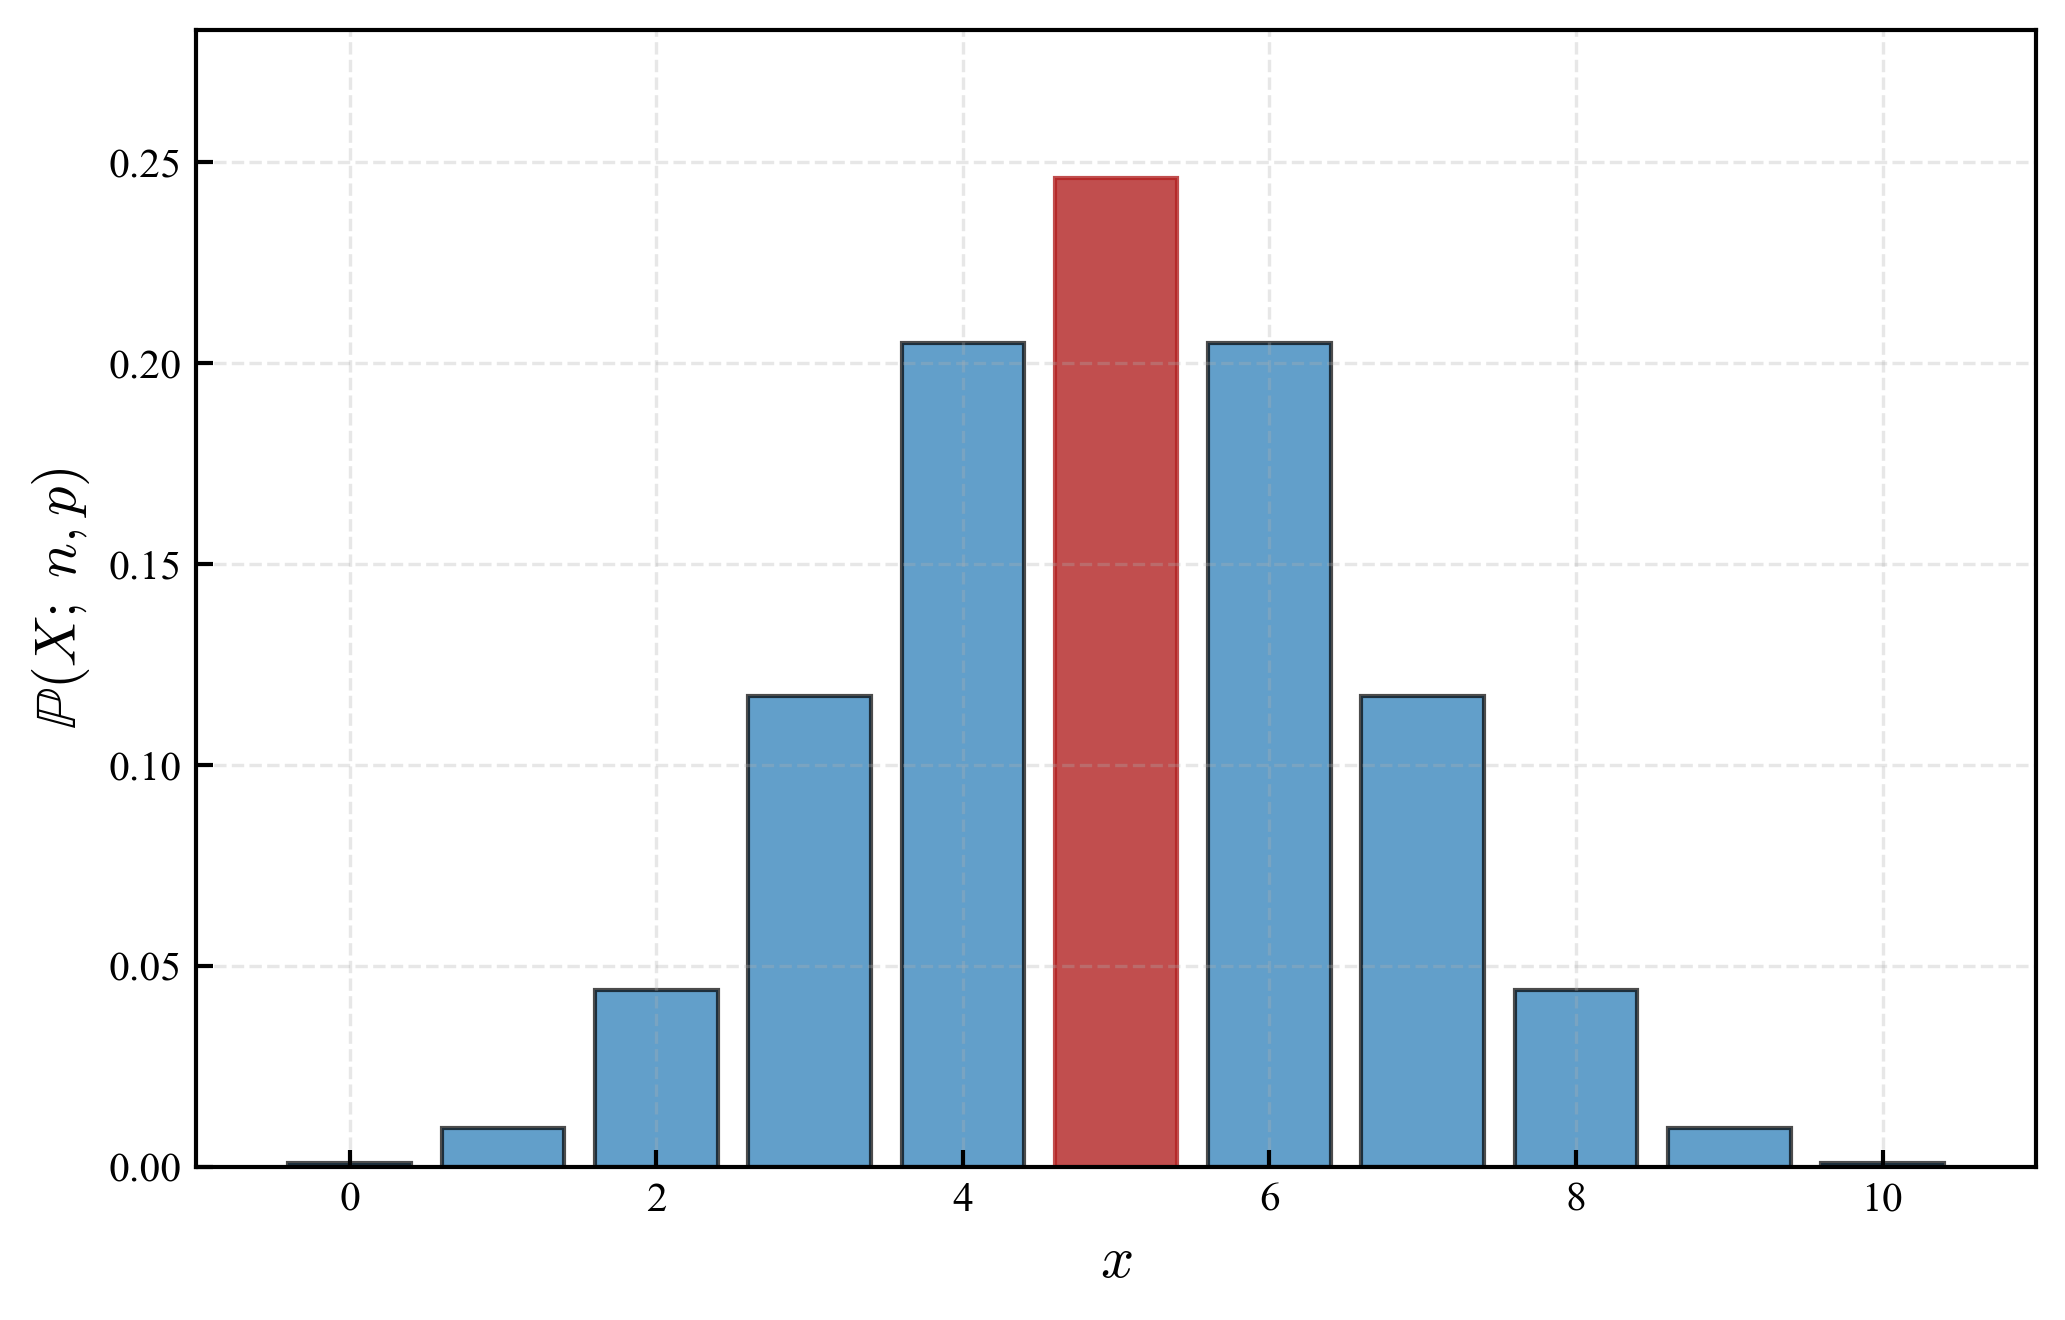
\includegraphics[width=0.7\textwidth]{figures/chapter2/binomial_1.png}
    \caption{Representation of the binomial distribution of a random variable $x$, given the total number of trials $n$ and the individual probability of success $p$.}
    \label{fig:binomial1}
\end{figure}

It was developed by Jacob Bernoulli in the 17th century while studying the probability of repeated Bernoulli trials. His work laid the foundation for the Law of Large Numbers

\subsection{Poisson distribution}

The next kind of random event we will discuss are the \textit{Poisson} distributed, named after the french mathematician Sim\'eon Denis Poisson, who tried to model to events that were random but with a known average rate, such as the number of people crossing a street per day, or the number of customers entering a store, or emails received per hour.
As a note, this distribution was introduced in quite recent times, in the early 19th century to model rare events. It is particularly useful for counting occurrences over a fixed interval of time or space.\\

The probability mass function for observing a number of events $x$ if we know the average rate $\lambda$ is:
\begin{equation}
    P(x; \lambda) = \frac{\lambda^x e^{-\lambda}}{x!},
\end{equation}
Again, let's consider a couple of examples to illustrate Poisson distributed events.

\begin{figure}[ht]
    \centering
    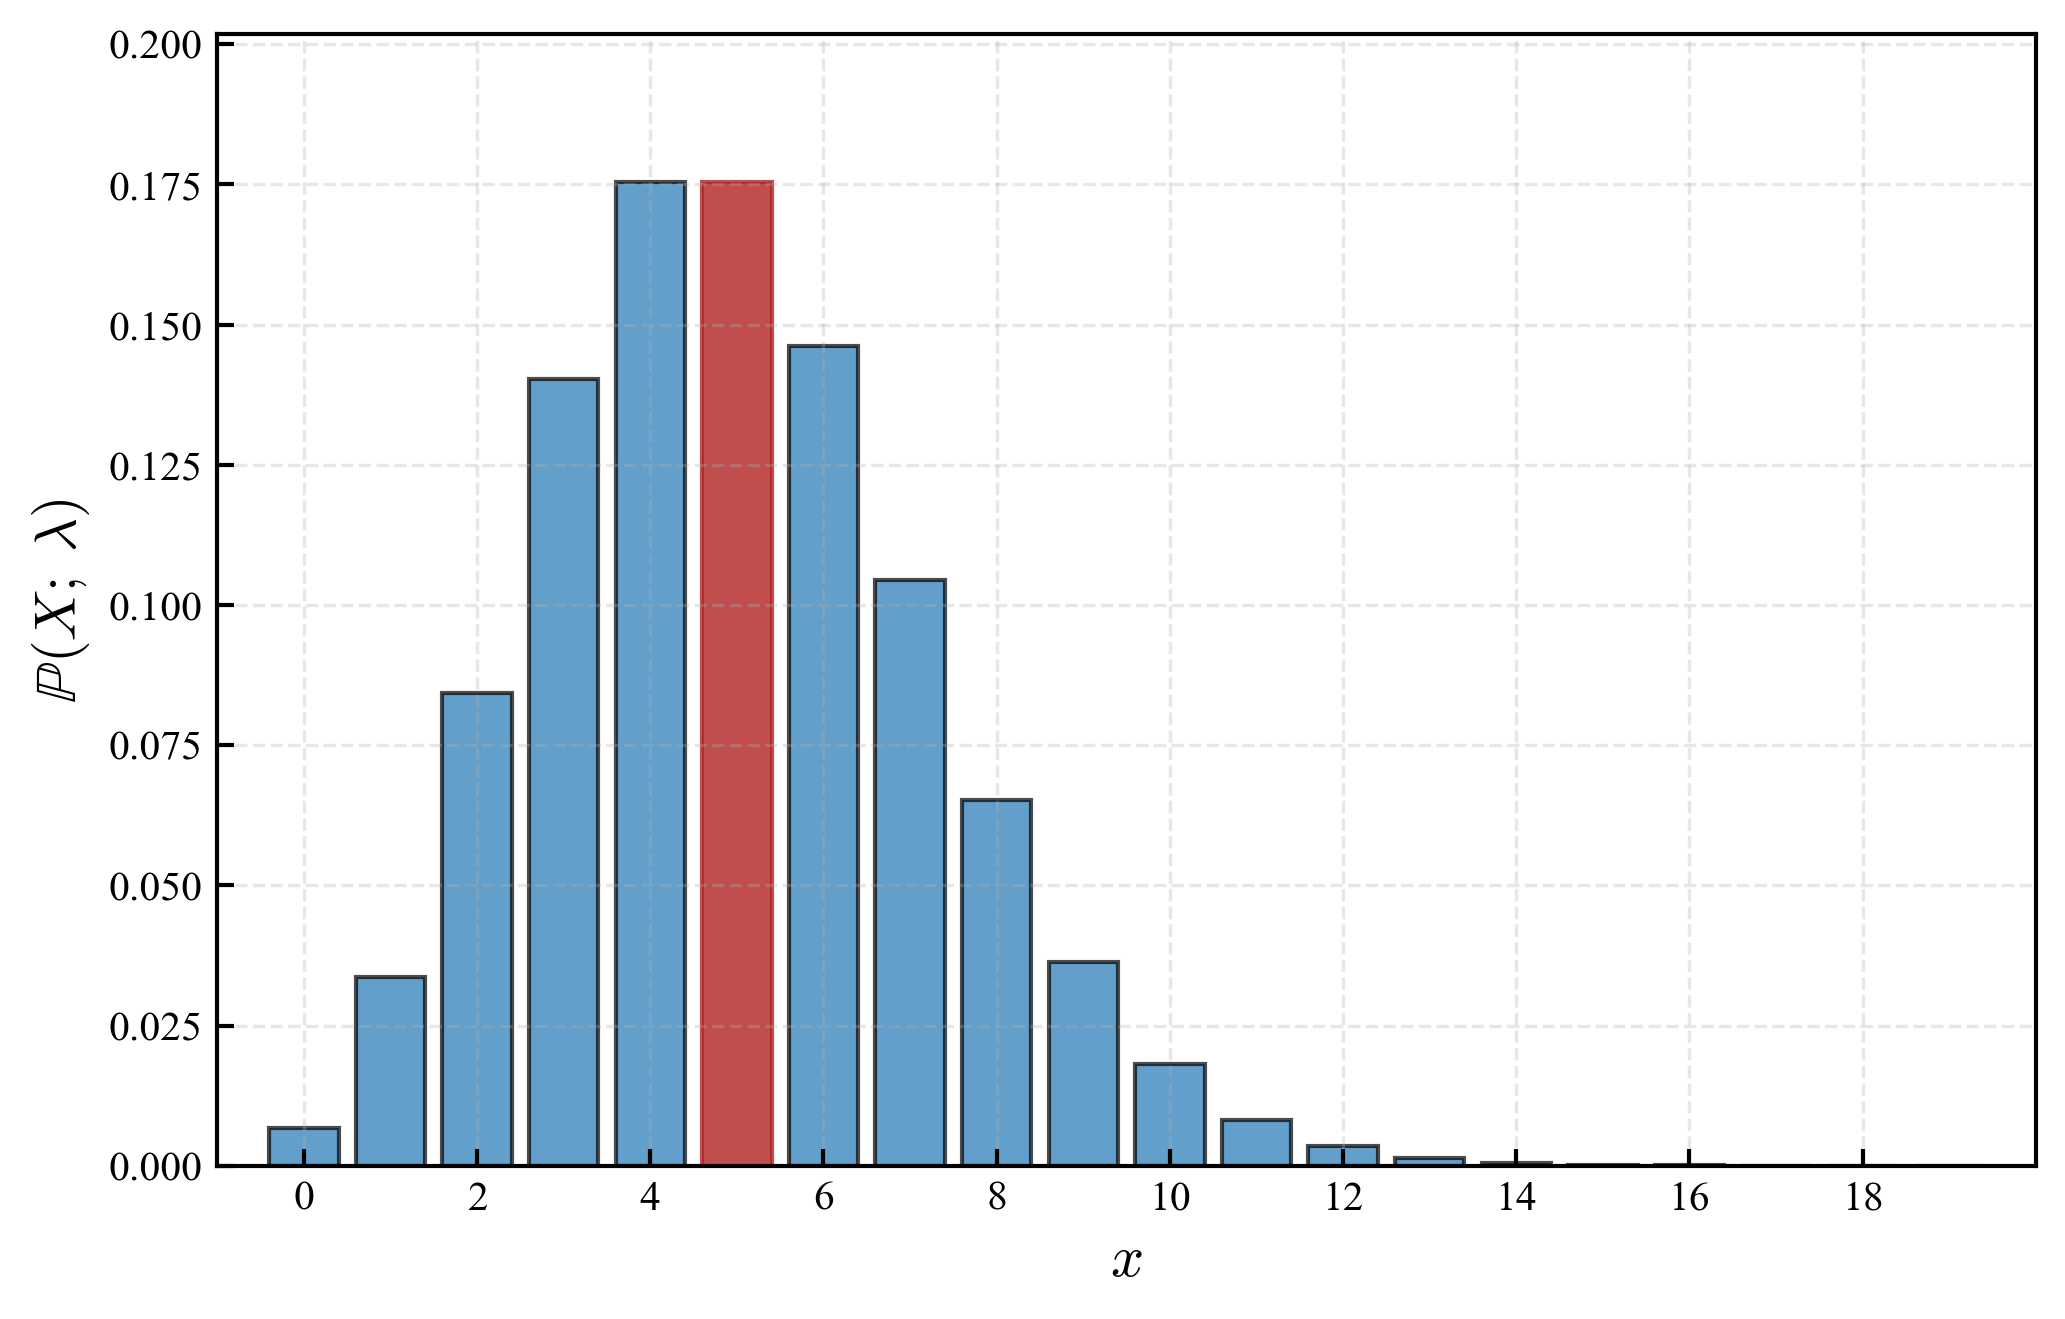
\includegraphics[width=0.7\textwidth]{figures/chapter2/poisson_1.png}
    \caption{Representation of the Poisson distribution of a random variable $x$, given the number of observations $\lambda$ as a parameter.}
    \label{fig:poisson1}
\end{figure}

\textbf{Example 1:} We would like to know the probability of observing exactly 5 cancer patients in a hospital over a week, if we know the average number ($\lambda = 3$) patients per week.
\begin{equation}
    P(x=5; \lambda = 3) = \frac{3^5 e^{-3}}{5!} = \frac{243 e^{-3}}{120} \approx 0.1008. \notag
\end{equation}\\

\textbf{Example 2:} Let's now ask a similar, but different question. So far, we have only focused on the probability of observing \textit{exactly} one particular outcome. But we could ask as well, what would be the probability observing 5 \textit{or less} cancer patients in that same hospital ($\lambda = 3$) patients per week.
\begin{align}
    P(x \leq 5; \lambda = 3) &= P(x=0; \lambda = 3) + P(x=1; \lambda = 3) + P(x=2; \lambda = 3) \notag \\
    &\quad + P(x=3; \lambda = 3) + P(x=4; \lambda = 3) + P(x=5; \lambda = 3) \notag
\end{align}\\

This is what we refer to as \textit{cumulative probability}, or \textit{cumulative distribution} [...].
\newpage

\section{Continuous random variables}

We will distinguish two main families of random events. These in which the number of possible outcomes is finite, or \textit{countable}, and the ones where the number of outcomes is \textit{uncountable}. The first ones will be named as \textit{discrete} events, while the second are normally referred to as \textit{continuous} [...]. \\

So far we have focused on discrete events, that is, scenarios where the number of possible outcomes was an integer number. Now we will encounter a second family of stochastic processes, the ones we will refer to as continuous. In the discrete case, we were implicitly using the frequentist definition of probability, as a number that represents the ratio of how many times we will observe a particular result, if we endlessly repeat [...].\\

But let's face now a different scenario. What would happen if we try to guess the probability of measuring something which does hace an infinite number of possible outcomes, spread on a continuous range? - e.g., the probability of measuring the height of a person an get 1.75 cm, or the temperature in a room and get 25 degrees, etc. Here we notice that, if we keep the definition of probability we used in the case of the Binomial, the Poisson, etc, we would get something like:

\begin{equation}
P(x = x_{0}) = \frac{\text{number of times I get $x_{0}$}}{\text{number of times I get any other result}}
\end{equation}

Note that now, the possible results are not just 1, 2, ..., n, but actually infinite more and spread over a \textit{continuous} range. The outcome of measuring a temperature could be the $T = 25$ we want, but also $T = 24.999$ and $T = 25.001$, and there are \textit{infinite} other possible results between these two. No matter how precise our measurement devices, are, between any pair of results, we would have an infinite number of cases where we obtain a different result. Hence, applying the frequentist definition of probability would lead to:

\begin{equation}
P(x = x_{0}) = \frac{\text{number of times I get $x_{0}$}}{\text{number of times I get any other result}} = \frac{n}{\infty} = 0
\end{equation}

We would get that the probability of obtaining \textit{any result} would be exactly zero.\\

Let's pause for a moment and think about what happened. At the very beginning of this chapter we said that the quantity $P(x)$ was used to represent information - also certainty, surprise - and computed using the frequentist approach, meaning the \textit{ratio of favorable cases and total cases}. But that was assuming we had a finite set or possibilities, or measure space.

\begin{itemize}
\item Discrete (coins, dice, counting) $\longrightarrow$ finite, \textit{countable} outcomes.
\item Continuous (temperature, energy, concentration, ...) $\longrightarrow$ infinite, \textit{uncountable} outcomes.
\end{itemize}

For such cases we will define a mathematical quantity, similar to that we called probability, which represents analogous information, but considering the fact we are dealing with a continuous event. We will call it \textit{probability density} or simply \textit{density}, and we will denote it with $f(x)$. Note that we can distinguish it from the probability in discrete events $P(x_{i})$, where we used the subscript $x_{i}$ to represent that the random variable could take just a finite set of values ($x_{1}$, $x{2}$, etc).

\begin{itemize}
\item Discrete (coins, dice, counting) $\longrightarrow$ Probability $P(x_{i})$ | $\sum_{i = 1}^{\infty} P(x_{i}) = 1$
\item Continuous (temperature, energy, concentration, ...) $\longrightarrow$ Probability density f(x) | $\int_{i = 0}^{\infty} f(x) dx = 1$
\end{itemize}

In the same way we imposed that probability needs to obey unitarity, we will impose that property in our recently defined probability density $f(x)$. The way we represent the sum for all possible cases in the continuous case, is just imposing that the integral of the function $f(x)$ is 1. This is just an example of \textit{normalization}, that we will explore further in Chapter 4 [...].

\subsection{Uniform distribution}

The uniform distribution represents events where all outcomes in an interval $[a, b]$ are equally likely [...].\\

The probability of observing a particular result $x$ in a given range $[a, b]$ is:

\begin{equation}
    f(x; a, b) = \frac{1}{b-a}, \quad a \leq x \leq b \; .
\end{equation}

\begin{figure}[ht]
    \centering
    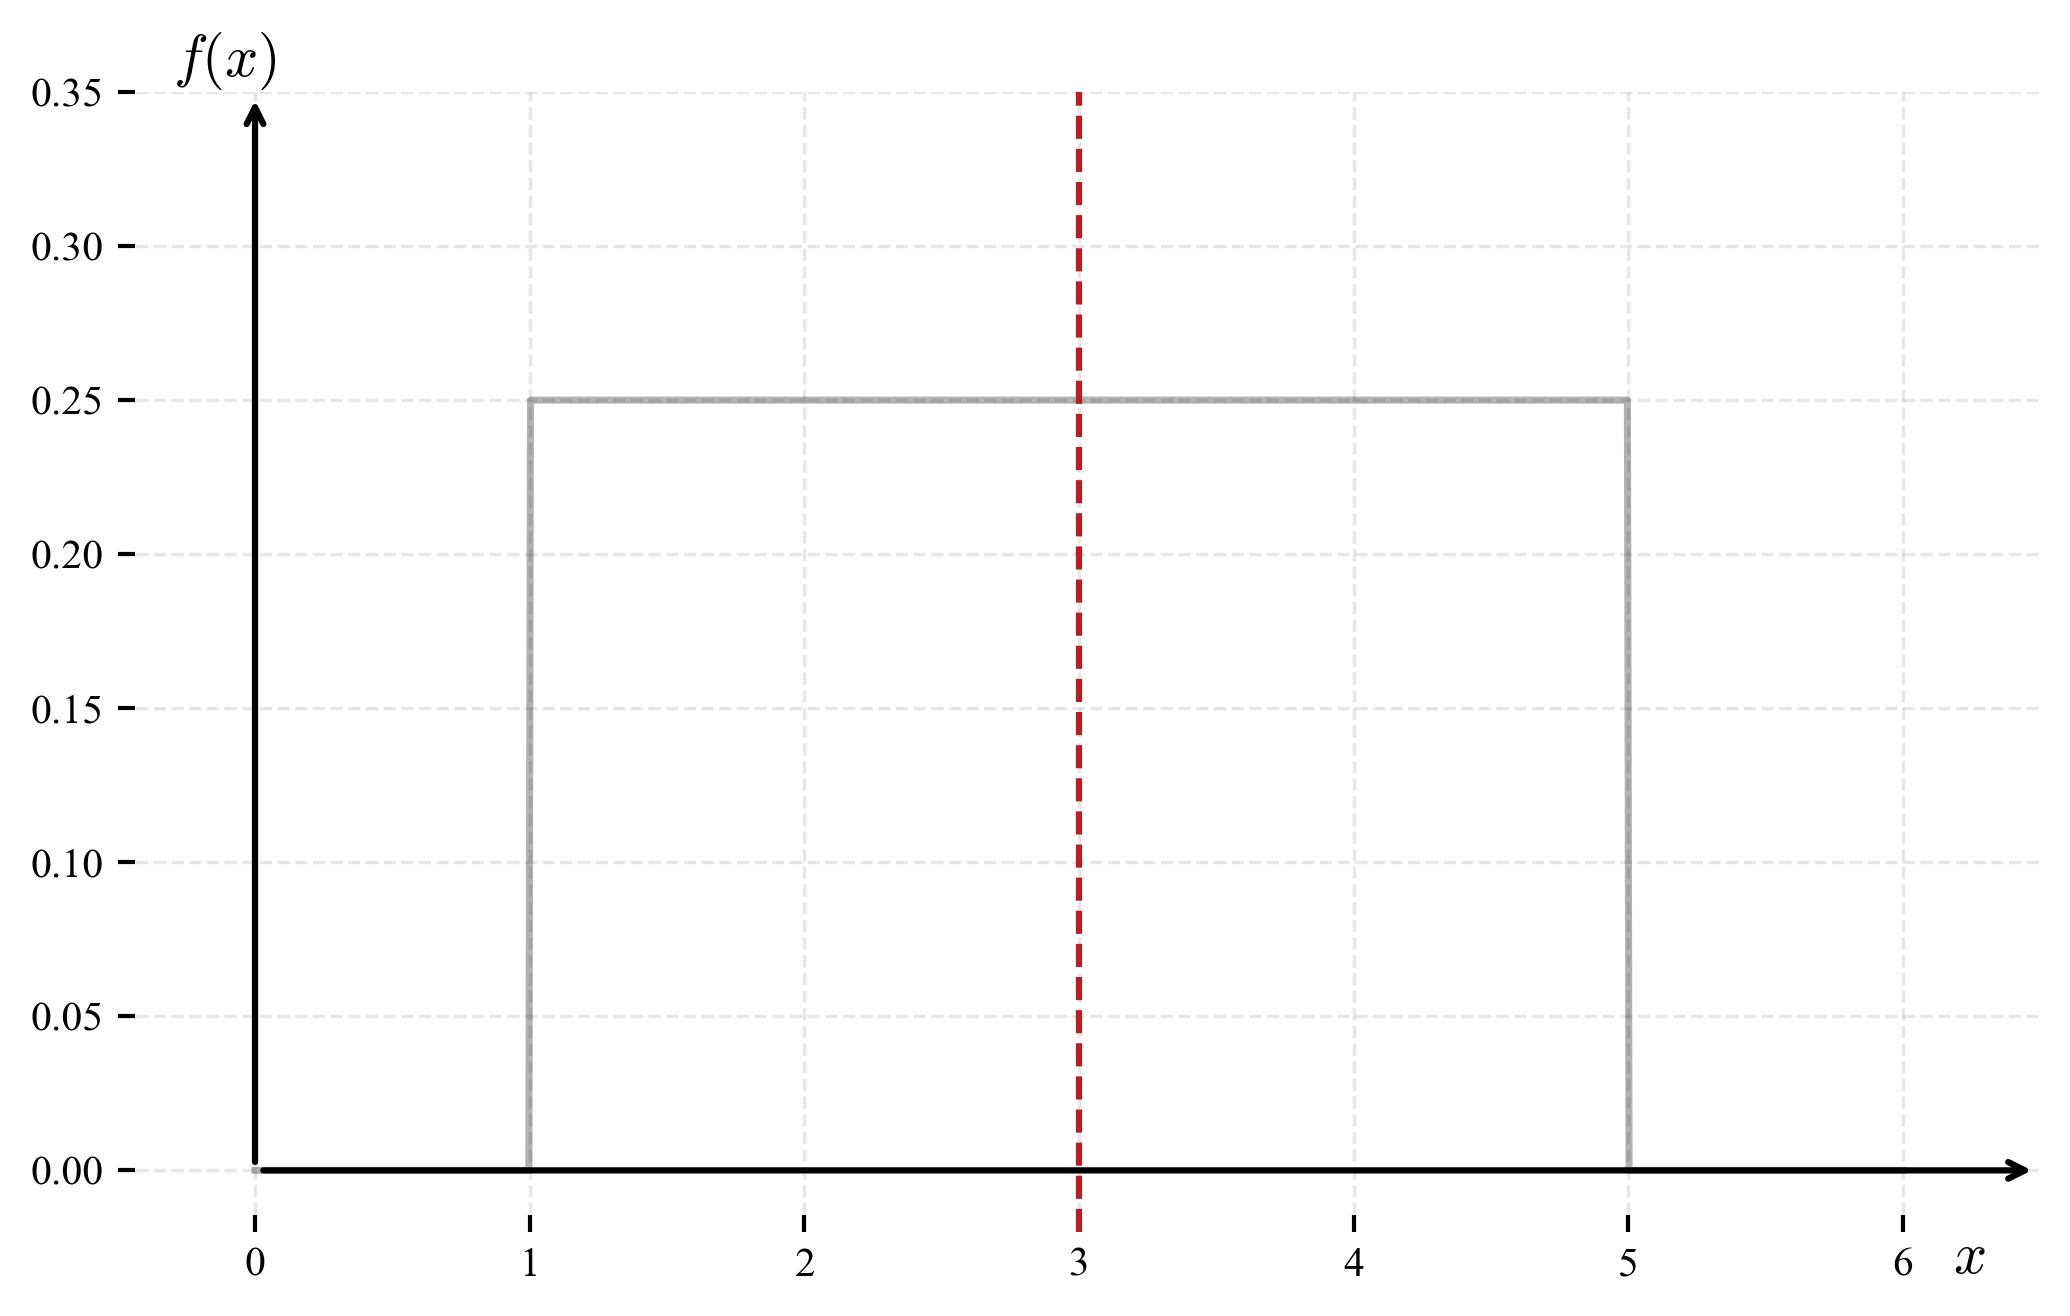
\includegraphics[width=0.7\textwidth]{figures/chapter2/uniform_1.png}
    \caption{Representation of the uniform distribution of a random variable $x$, given the boundaries $a$, $b$.}
    \label{fig:uniform1}
\end{figure}

\begin{figure}[ht]
    \centering
    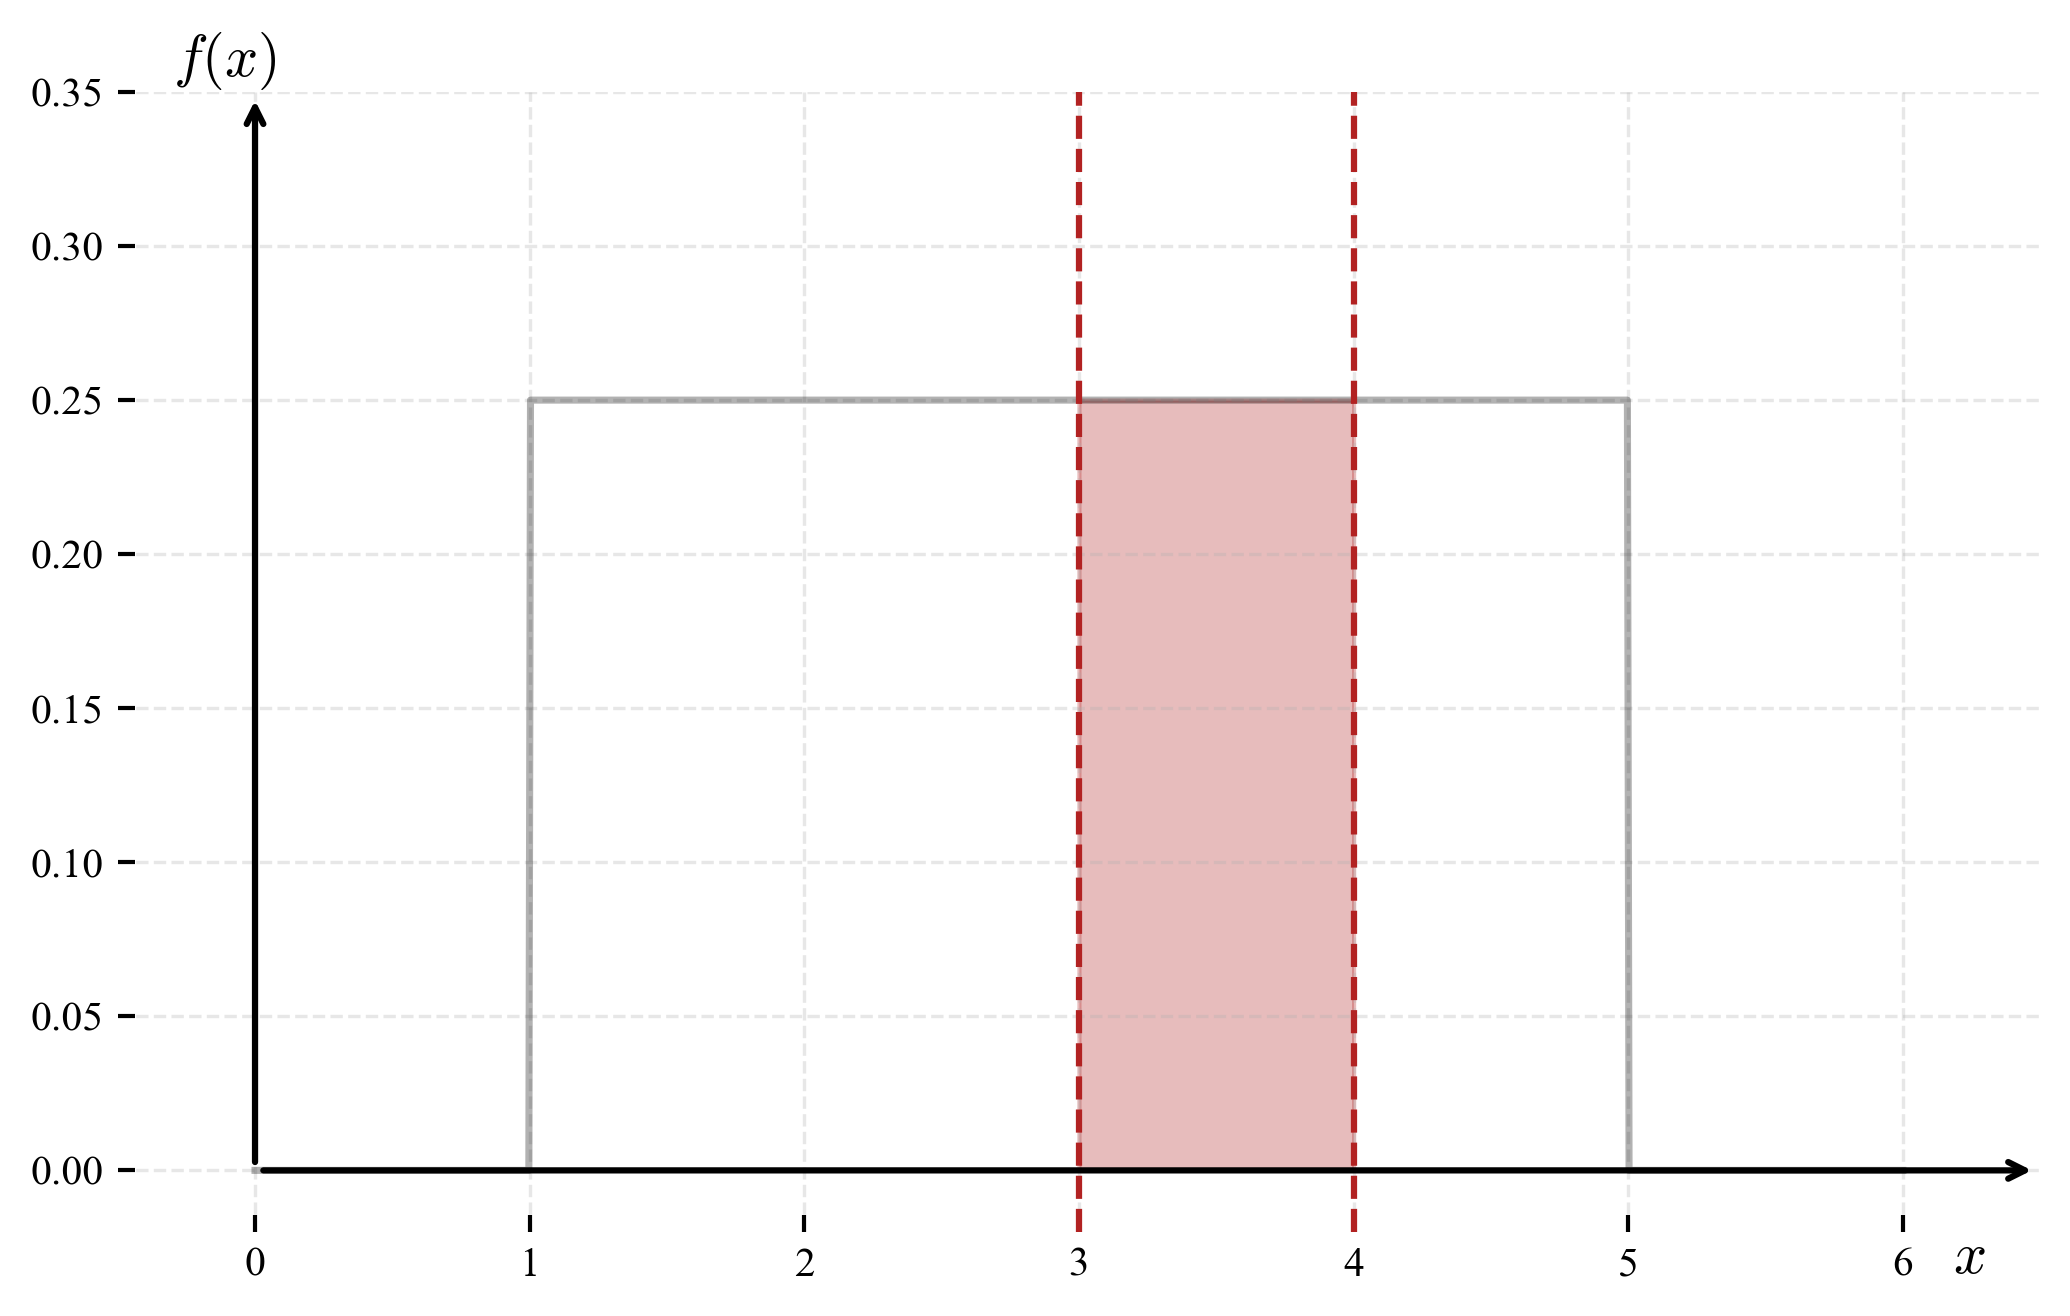
\includegraphics[width=0.7\textwidth]{figures/chapter2/uniform_2.png}
    \caption{Representation of the uniform distribution of a random variable $x$, given the boundaries $a$, $b$.}
    \label{fig:uniform1}
\end{figure}

\newpage

\subsection{Gaussian distribution}
Introduced by Carl Friedrich Gauss, the normal distribution became central to statistics due to the Central Limit Theorem (CLT). It describes how averages of large samples tend to form a bell-shaped curve. Intuitively, many natural and social phenomena follow a normal distribution, such as human heights and test scores [...].\\

The probability density function is:
\begin{equation}
    f(x; \mu, \sigma) = \frac{1}{\sigma \sqrt{2\pi}} e^{-\frac{(x-\mu)^2}{2\sigma^2}} \; .
\end{equation}

\begin{figure}[ht]
    \centering
    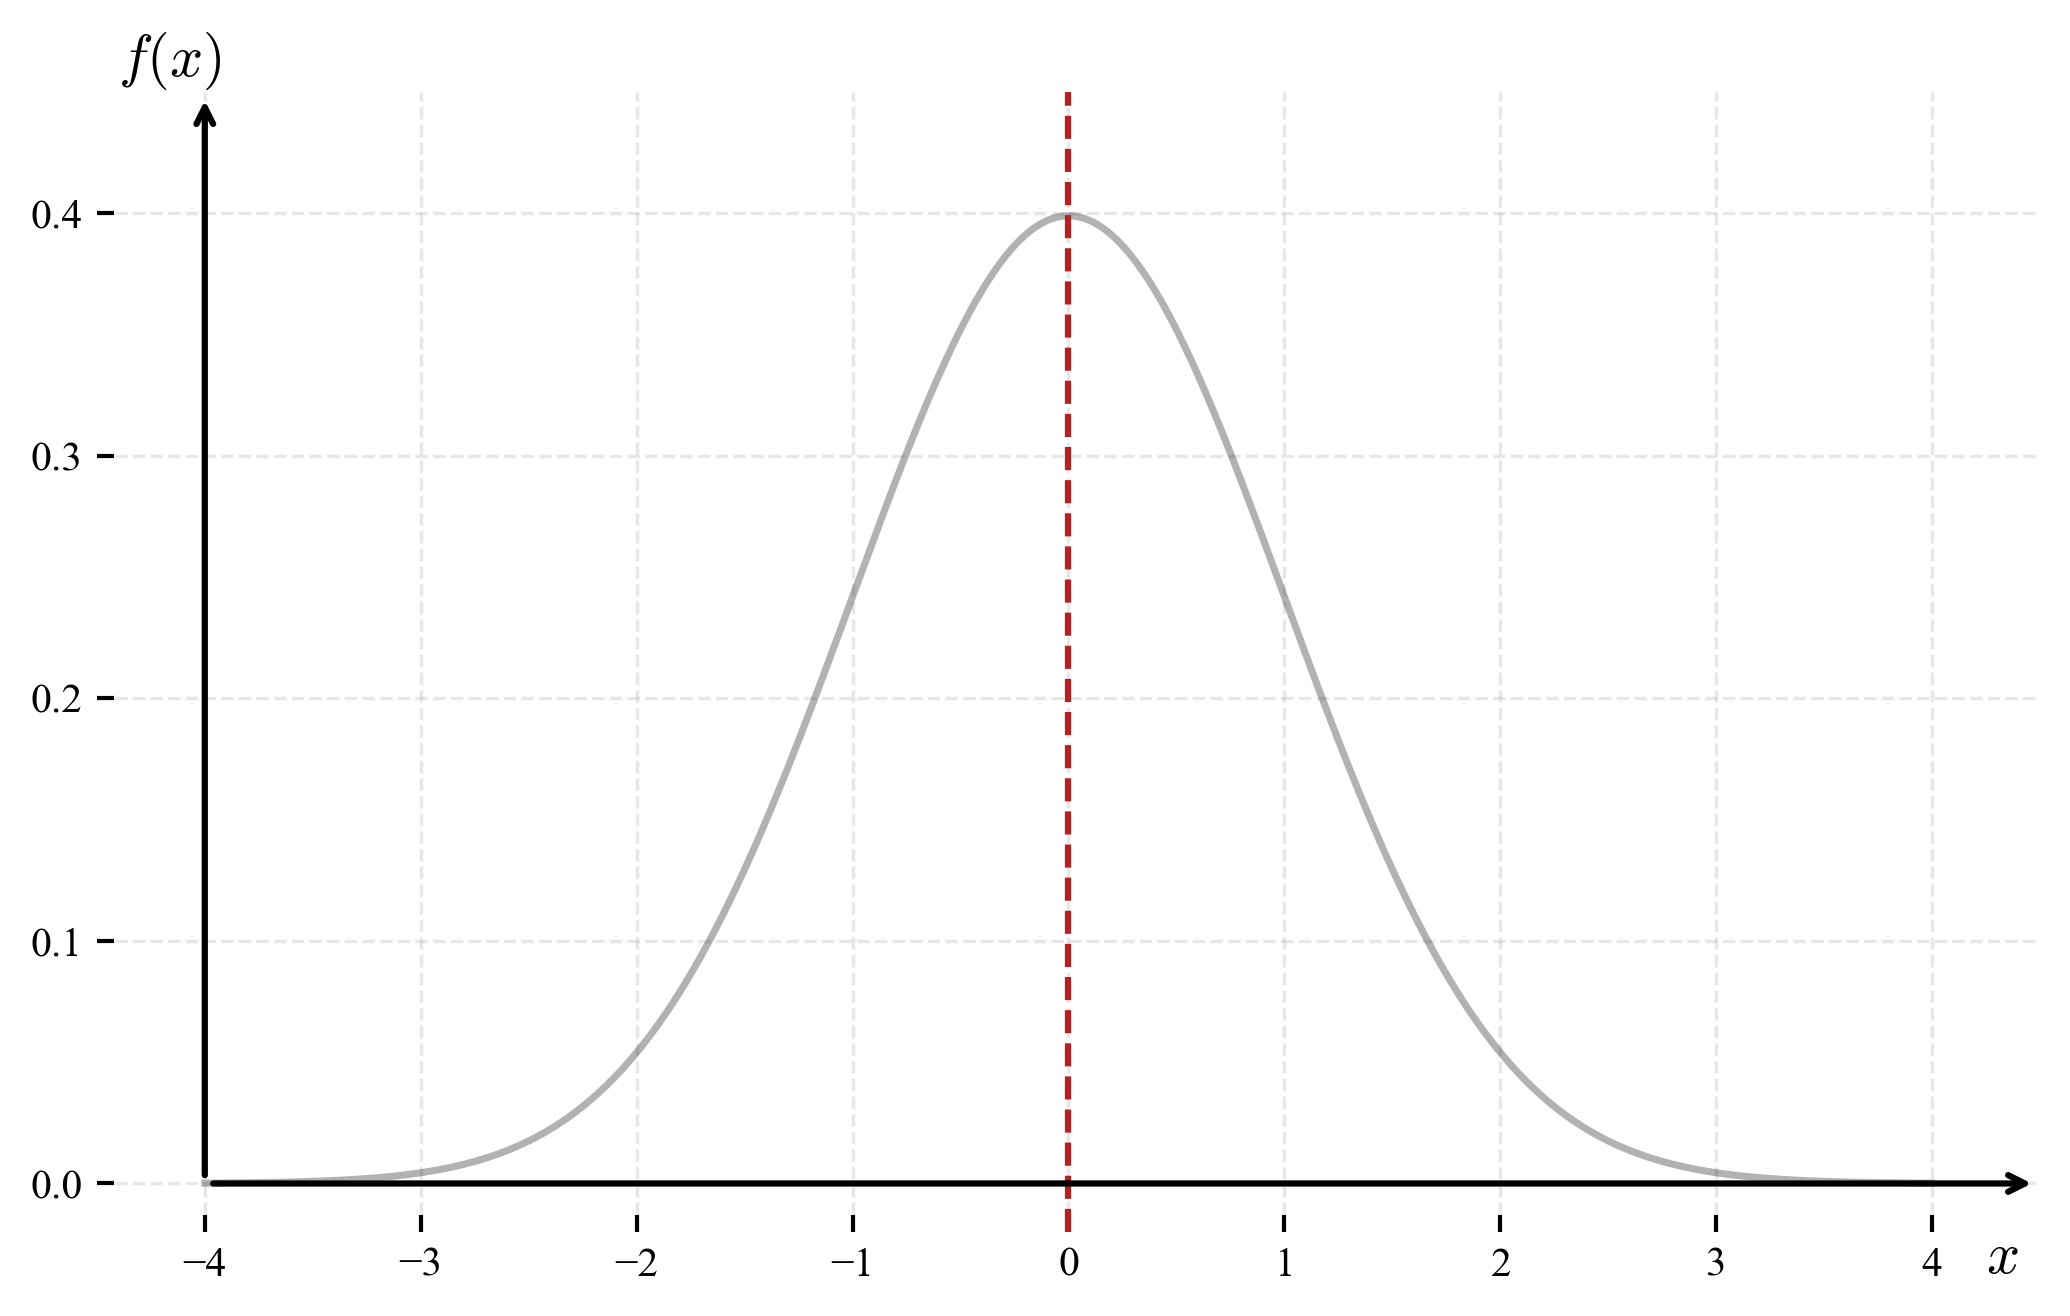
\includegraphics[width=0.7\textwidth]{figures/chapter2/gaussian_1.png}
    \caption{Representation of the gaussian distribution of a random variable $x$, given the mean value $\mu$ and standard deviation $\sigma$ parameters.}
    \label{fig:gaussian1}
\end{figure}

\begin{figure}[ht]
    \centering
    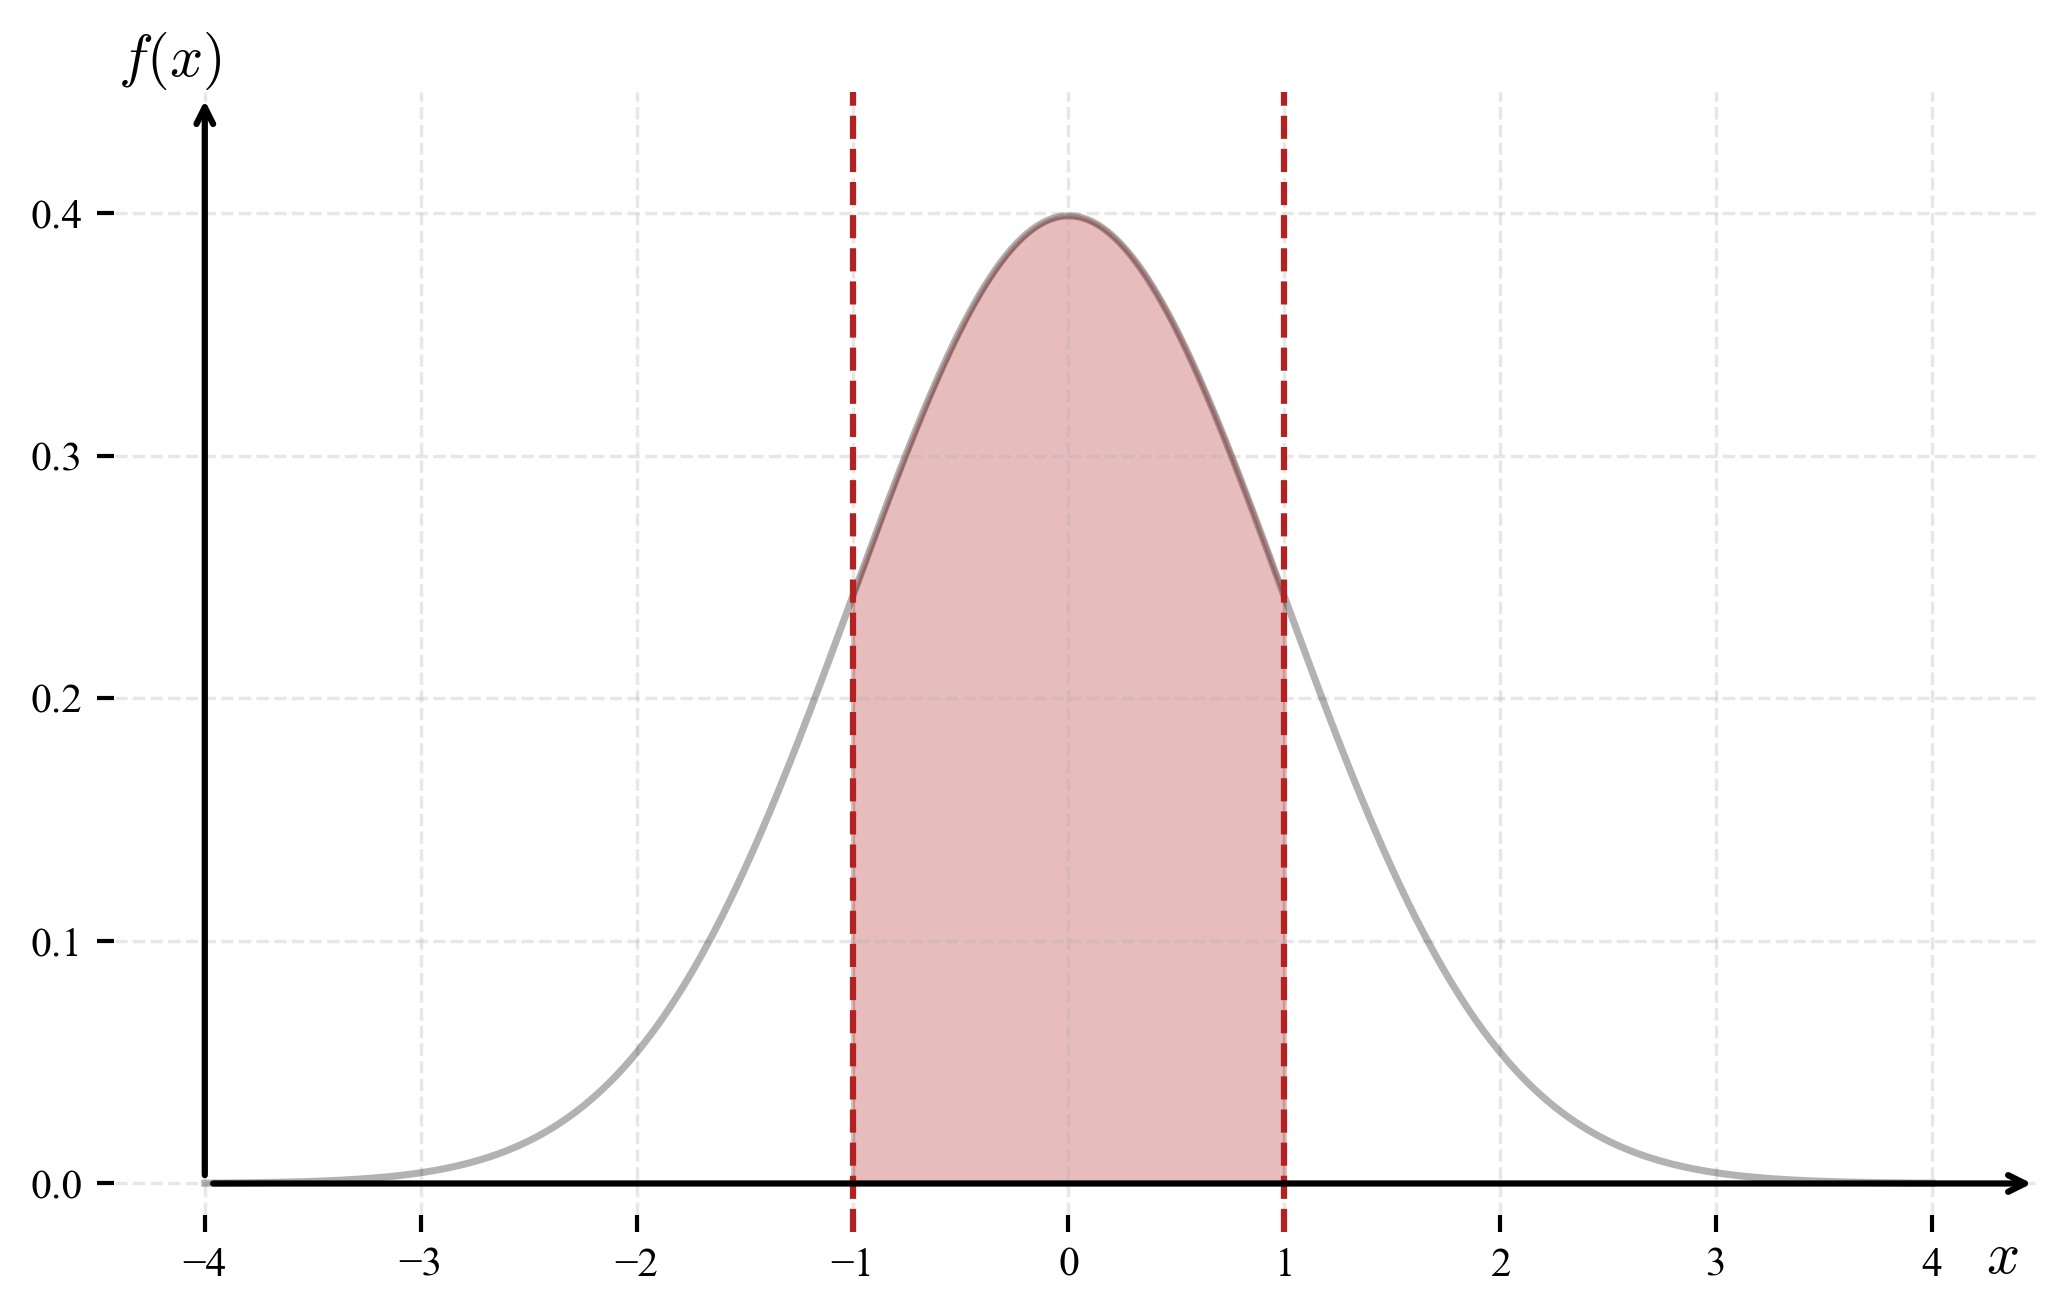
\includegraphics[width=0.7\textwidth]{figures/chapter2/gaussian_2.png}
    \caption{Representation of the gaussian distribution of a random variable $x$, given the mean value $\mu$ and standard deviation $\sigma$ parameters.}
    \label{fig:gaussian1}
\end{figure}

\newpage

\subsection{Exponential distribution}
The exponential distribution models waiting times between. Intuitively, it describes situations where the probability of waiting a certain time between events remains constant, such as time between bus arrivals [...].\\

The probability density function is:
\begin{equation}
    f(x; \lambda) = \lambda e^{-\lambda x}, \quad x \geq 0 \; .
\end{equation}

\begin{figure}[ht]
    \centering
    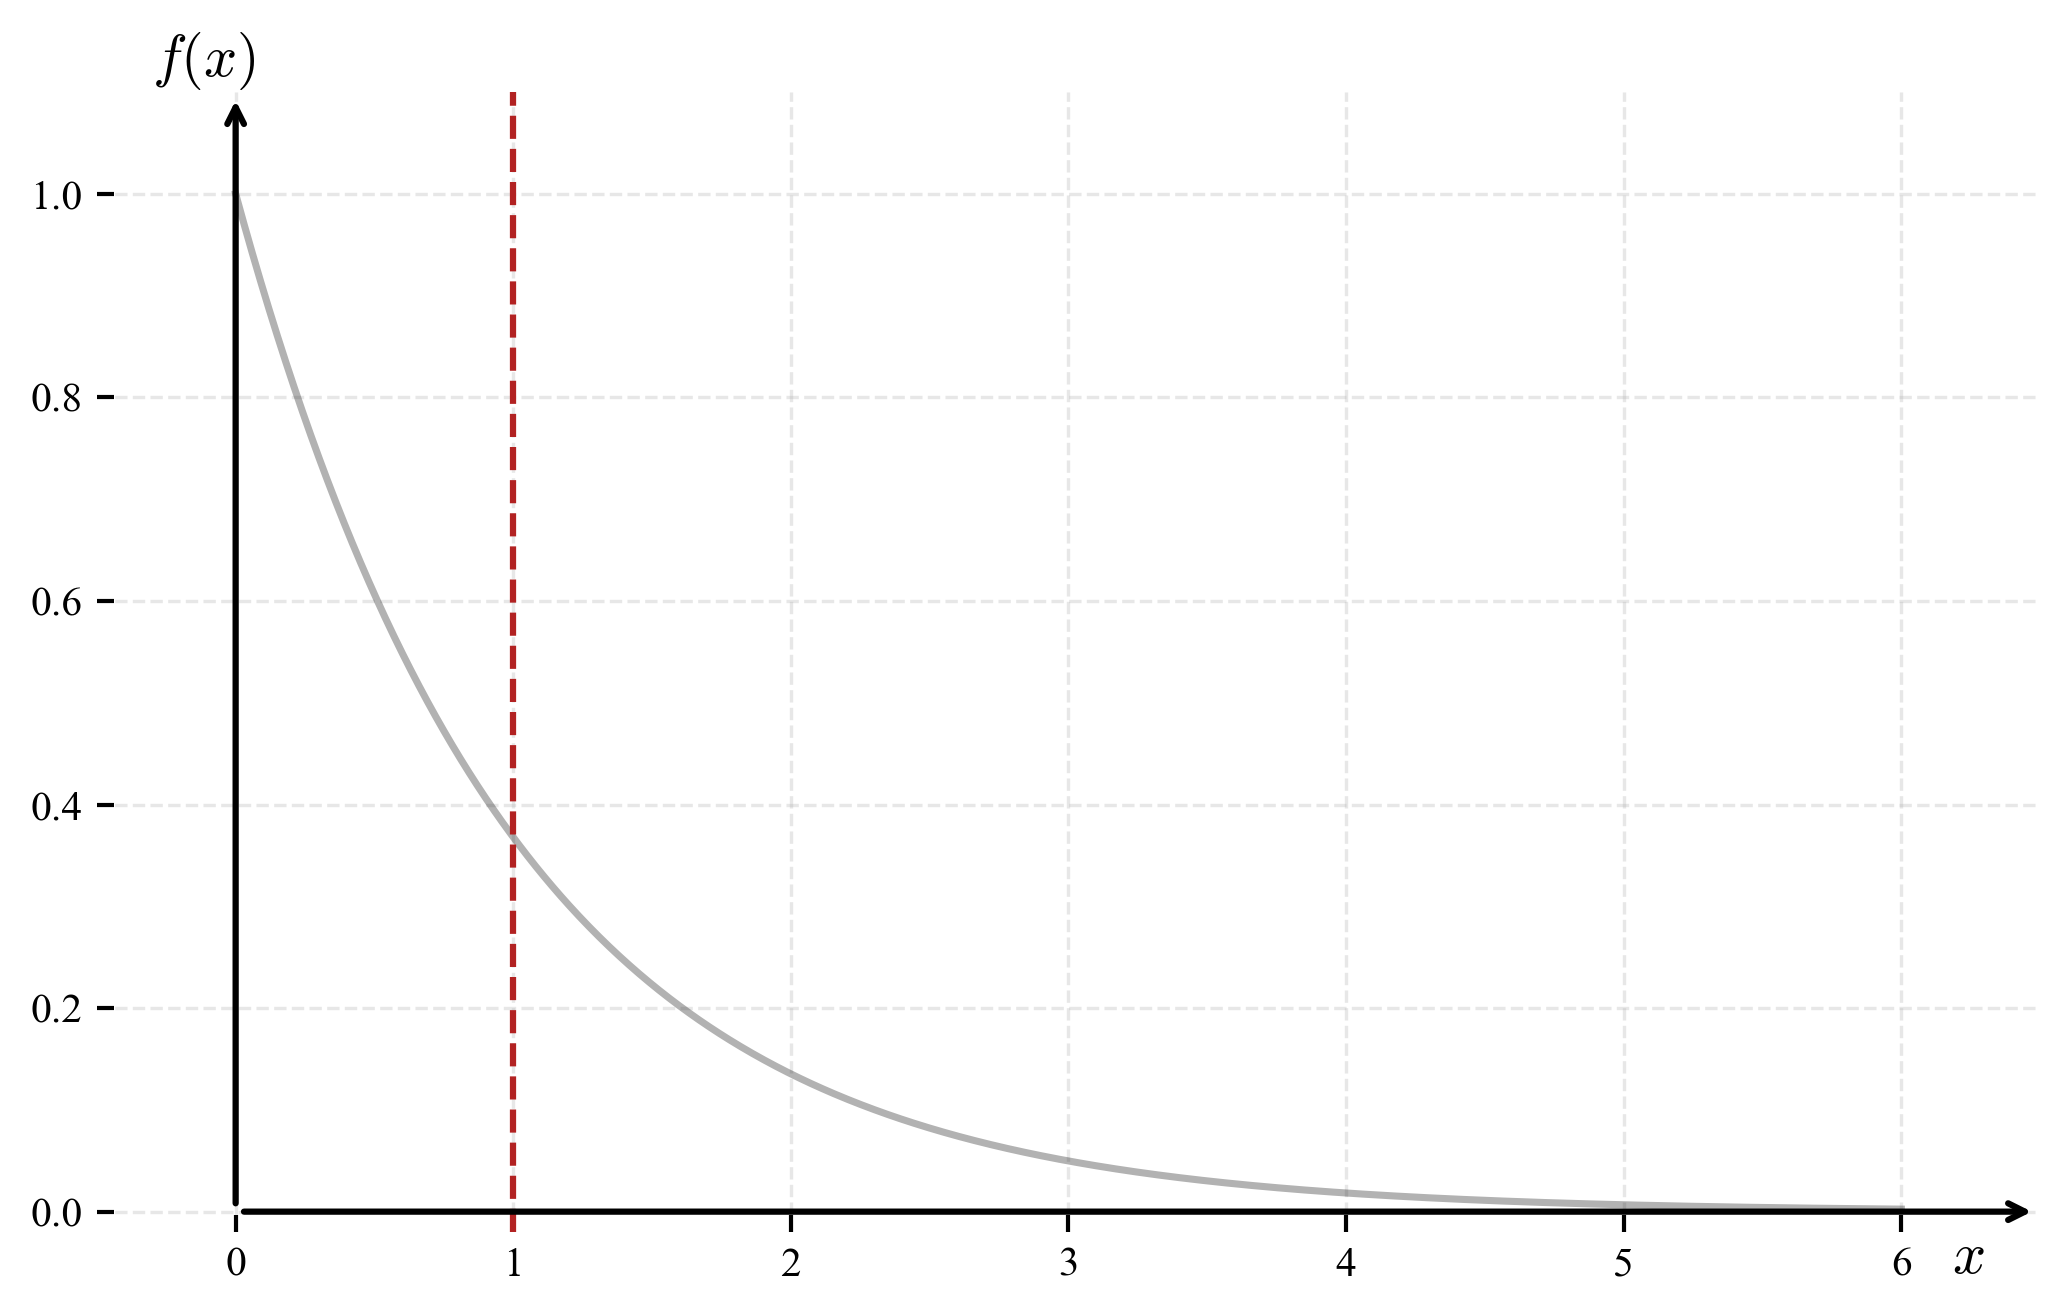
\includegraphics[width=0.7\textwidth]{figures/chapter2/exponential_1.png}
    \caption{Representation of the exponential distribution of a random variable $x$, given the decay rate $\lambda$.}
    \label{fig:exponential1}
\end{figure}

\begin{figure}[ht]
    \centering
    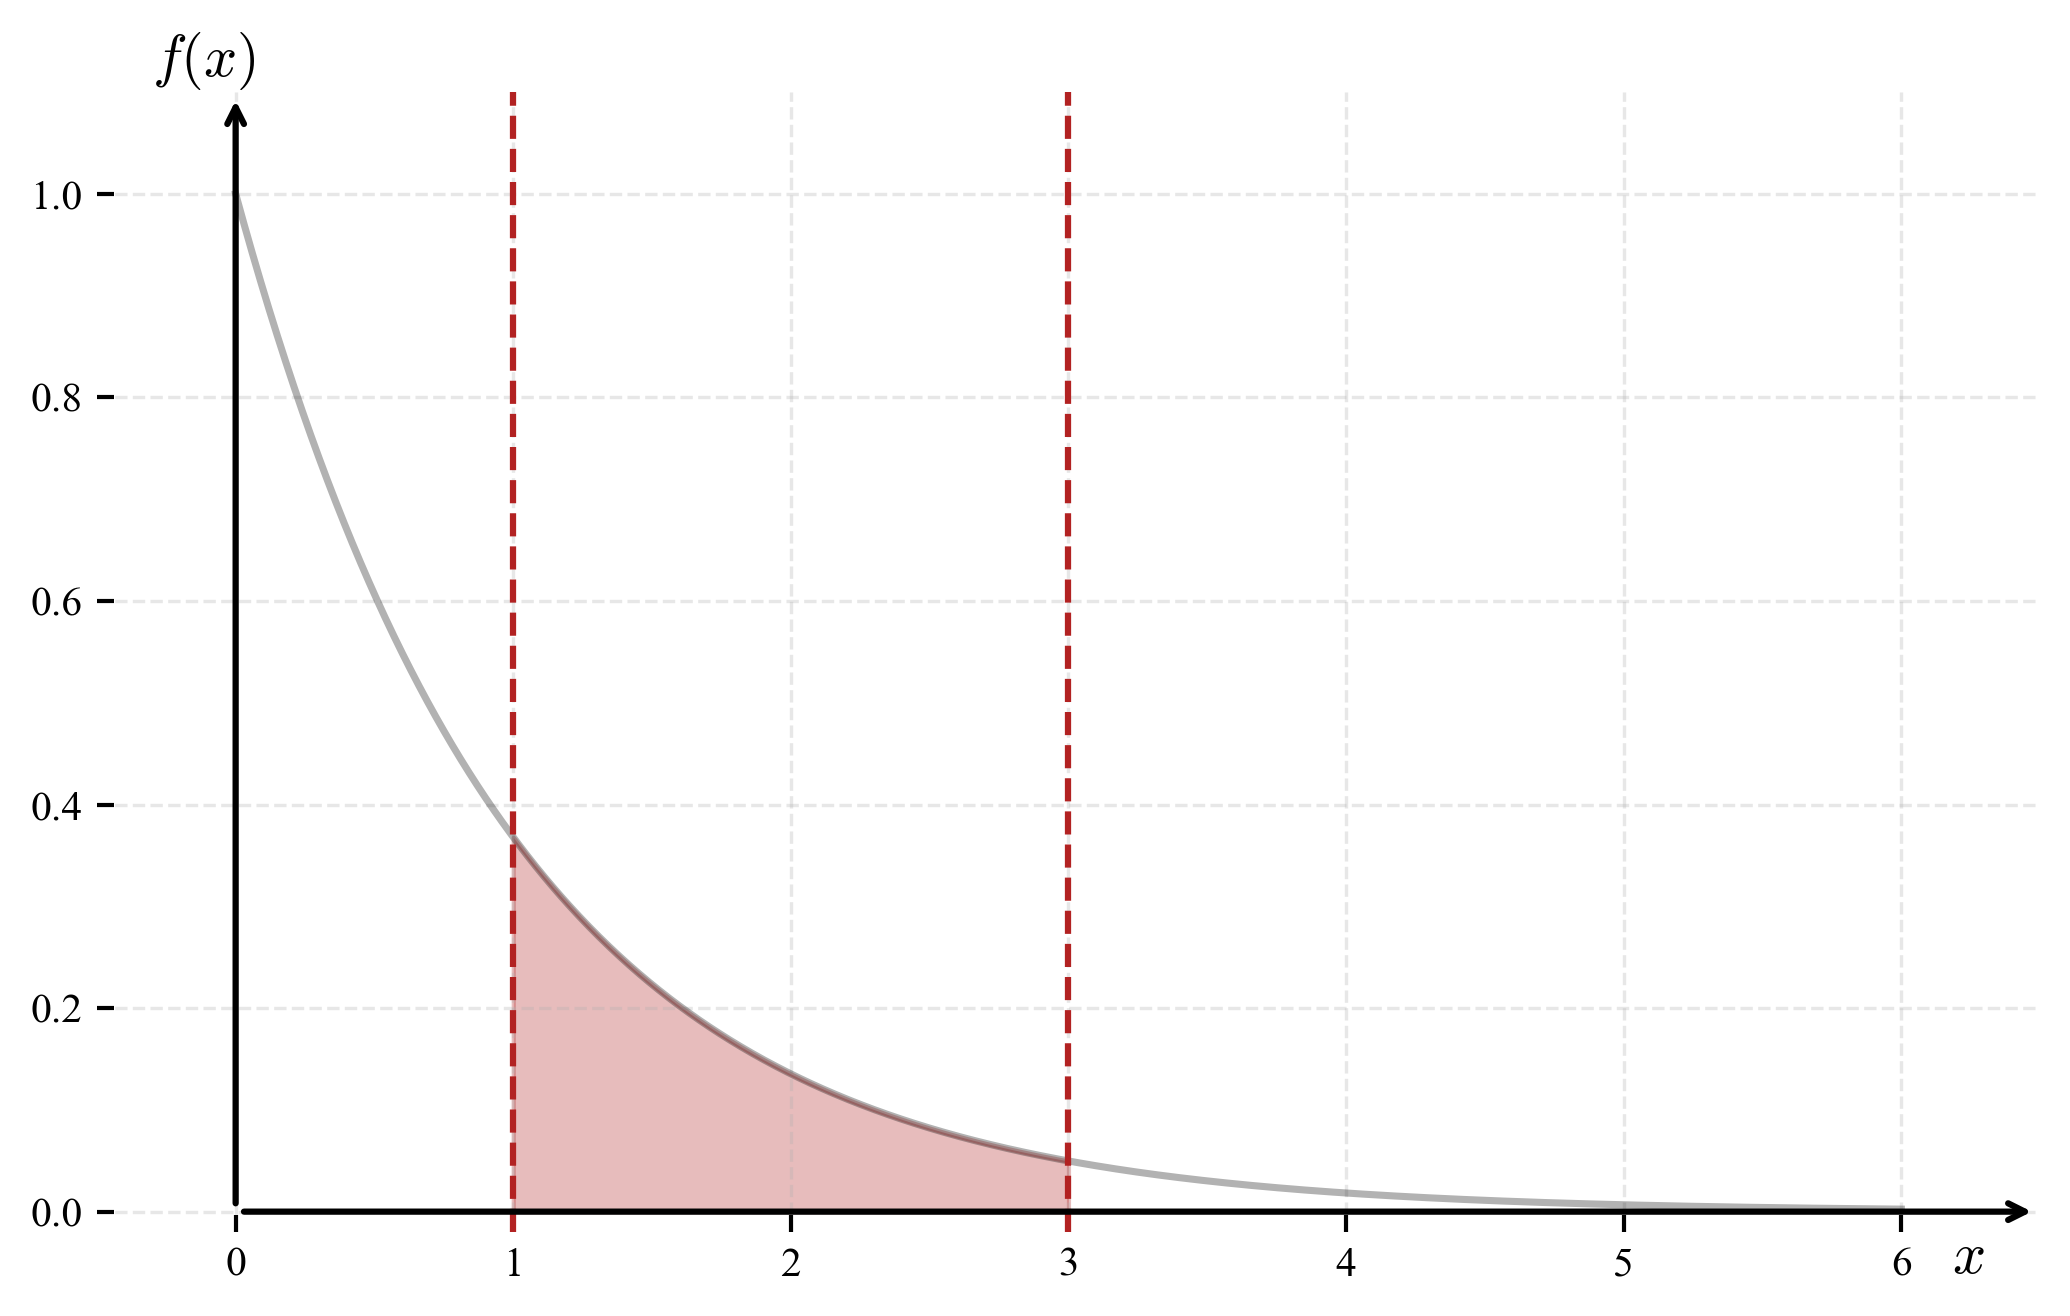
\includegraphics[width=0.7\textwidth]{figures/chapter2/exponential_2.png}
    \caption{Representation of the exponential distribution of a random variable $x$, given the decay rate $\lambda$.}
    \label{fig:exponential1}
\end{figure}

\newpage

\subsection*{Exercises}

\textbf{1.} Exercise [...].\\

\textbf{2.} Exercise [...].\\

\textbf{3.} Exercise [...].\\

\newpage

\subsection*{Solutions}

\textbf{1.} Solution [...].\\

\textbf{2.} Solution [...].\\

\textbf{3.} Solution [...].\\




% Chapter - Parameter estimation .........................................................................................................................................................
\chapter{Parameter estimation}

\epigraph{\textit{Numbers have an important story to tell. They rely on us to give them a voice.}}{— Florence Nightingale}

\section{Prediction vs inference}

In the previous chapters we have introduced the mathematical theory of probability. We have developed a series of tools, a \textit{theory}, which enables us to make predictions in stochastic processes. But, contrary to what is normally explain in introductory courses, science is not always headed in the theory - prediction - experiment direction. There can be cases, as we will soon see, where hypothesis are formulated for a given phenomena, and no prediction is made. In such cases, it is from measurement that we will try to see, or \textit{infer} if a given set of assumptions are compatible with the obtained data. Indeed, most modern data analysis and hypothesis testing lie in the \textit{inferential} statistics, rather than \textit{predictive} probability [...].\\

Inference seeks to explain why and how variables relate. The key idea is causality and interpretability: given a some set of observations, inference aims to answer questions such as: Does smoking cause lung cancer, or is the correlation due to other confounding factors? How does an increase in temperature affect ice cream sales? What are the most significant predictors of house prices? The difference between prediction and inference has been a topic of interest in statistics and data science for centuries. While both concepts involve drawing conclusions from data, their goals, methodologies, and historical development differ significantly [...].\\

The roots of inference trace back to classical statistics, particularly the work of Laplace (1749–1827) Gauss (1777–1855), who developed probability theory and the method of least squares. Their work laid the foundation for statistical inference, which aims to understand relationships between variables and make generalizable conclusions about populations from samples. For example, Laplace used probability theory to estimate the population of France, introducing Bayesian inference, which provides a framework for updating beliefs based on observed data. Gauss contributed the normal distribution and least squares estimation, which became essential for making inferences about unknown parameters.

Statistical techniques such as hypothesis testing, confidence intervals, and regression analysis aim to understand and describe these relationships. The emphasis lies on estimating parameters and determining statistical significance rather than simply making accurate predictions. A classic example is Ronald Fisher (1890–1962), who developed maximum likelihood estimation (MLE) to infer parameters of probability distributions. [...].\\

Prediction focuses on accuracy and generalization rather than explaining causality. The goal is to create a model that performs well on new, unseen data, even if the underlying relationships between variables are not fully understood. For example, in modern deep learning, neural networks can recognize faces with high accuracy but offer little interpretability in how they make decisions. Unlike inference, which aims to understand why a pattern exists, prediction is about making the best possible guess given the available data. Focus shifted from understanding relationships to optimizing models that generalize well to unseen data. In 2001, Leo Breiman, in his seminal paper "Statistical Modelling: The Two Cultures," highlighted the distinction, arguing that traditional statistics emphasized inference, whereas modern machine learning prioritized prediction.\\

\section{Parameters and variables}
Another key difference we will discuss now, and quite a subtle one from the mathematical perspective, is that one between a \textit{variable} and a \textit{parameter}. Consider the example of a binomial experiment, e.g. tossing coins and asking for the probability of measuring a specific number of heads. There, we would write it as 

\begin{equation}
    P(x; n, p) = \binom{n}{k} p^x (1-p)^{n-x},
\end{equation}
where $n$ is the number of trials and $p$ is the probability of success.\\

In our previous examples, we have treated just $x$ as our variable of interest, but we could think about P as a function of three independent variables. The number of times we want to observe heads, the total number of trials, and the probability of success for each toss. Normally, we will call \textit{parameters}, to all these variables we will freeze for the purpose of our calculations, and either consider them either known, or fit them from data [...].
 
 \newpage 
 
\section{The Law of Large Numbers}

The \textit{Law of Large Numbers} (LLN) is a fundamental theorem in probability theory that formalizes the idea that averages computed from large samples tend to stabilize, and approximate the expected value of the underlying random process. In essence, it states that as the number of trials increases, the sample mean of a sequence of random observations converges to the population mean. This result justifies the very concept of statistical average, and forms the basis for almost all of empirical science, data analysis, and applied statistics.

\medskip

The Law of Large Numbers expresses a powerful kind of regularity that emerges from randomness. Suppose you flip a fair coin many times. While the outcome of any single flip is uncertain, the proportion of heads observed in the long run should converge to 0.5. The underlying reason for this stabilization lies in the independence of trials and the additivity of probability: large samples ``dilute" random fluctuations and reveal the structure of the distribution. The LLN can be understood as a consequence of the averaging process: the sum of independent random deviations around the mean tends to cancel out as the sample size increases, allowing the average to settle around its expected value.

\medskip

The earliest version of the Law of Large Numbers was proved by {Jacob Bernoulli} in 1713, posthumously published in his \textit{Ars Conjectandi}. He proved that the proportion of successes in a sequence of independent Bernoulli trials converges in probability to the success probability. This became known as the \textit{Weak Law of Large Numbers} (WLLN). In the 19th and 20th centuries, the LLN was generalized and refined. Russian mathematician Pafnuty Chebyshev extended the law beyond Bernoulli trials by introducing moment inequalities. Later, it was again Kolmogorov who provided a stronger formulation, the \textit{Strong Law of Large Numbers} (SLLN) - which guarantees almost sure convergence of the sample mean to the expected value under broader conditions.

The Law of Large Numbers states that as the sample size increases, the sample mean approaches the expected value. Formally, if $X_1, X_2, \dots, X_n$ are independent and identically distributed (i.i.d.) random variables with expected value $\mathbb{E}[X] = \mu$, then:

\begin{equation}
    \bar{X}_n = \frac{1}{n} \sum_{i=1}^{n} X_i \to \mu \quad \text{as } n \to \infty.
\end{equation}

Consider flipping a fair coin multiple times. The proportion of heads observed converges to 0.5 as the number of flips increases. This illustrates that the observed average stabilizes around the theoretical probability.

\medskip

The Weak Law can be phrased as follows. Let $x_1, x_2, \dots, x_n$ be a sequence of independent and identically distributed (i.i.d.) random variables with finite expected value $\mu = \mathbb{E}[X_i]$. We could define the sample mean as we just learned in previous section:

\begin{equation}
	\overline{x}_n = \frac{1}{n} \sum_{i=1}^n n_i.
\end{equation}

Then, the \textit{Weak Law of Large Numbers} states that for any $\varepsilon > 0$,

\begin{equation}
	\lim_{n \to \infty} \mathbb{P}\left( \left| \overline{X}_n - \mu \right| > \varepsilon \right) = 0.
\end{equation}

This means that sample mean $\overline{x}_n$ converges to the true value $\mu$ ias we increase the number of trials, $n \to \infty$.

\medskip

The Strong Law: under the same conditions, and with the additional requirement that $mathbb{E}[|x_i|] < \infty$, the \textbf{Strong Law of Large Numbers} states that:

\begin{equation}
	\mathbb{P}\left( \lim_{n \to \infty} \overline{X}_n = \mu \right) = 1.
\end{equation}

This is a stronger mode of convergence known as \emph{almost sure convergence}, meaning that the sequence \( \overline{X}_n \) converges to \( \mu \) with probability 1. Kolmogorov proved this version in 1933 using tools from measure theory, laying the foundation for modern probability theory.

\medskip

\textbf{Example}: tossing coins

Let \( X_i \) be a fair coin flip, coded as \( X_i = 1 \) for heads and \( X_i = 0 \) for tails. Then:

\[
	\mu = \mathbb{E}[X_i] = 0.5.
\]

Now flip a coin \( n = 10 \), then \( n = 50 \), then \( n = 500 \) times. At each step, compute the sample mean:

\[
	\overline{X}_n = \frac{1}{n} \sum_{i=1}^n X_i.
\]

You will observe that \( \overline{X}_n \) fluctuates at first, but as \( n \) increases, the value stabilizes near \( 0.5 \). This is a manifestation of the Law of Large Numbers: although the outcome of individual trials is unpredictable, the average of many trials is highly predictable and converges toward the expected value.

\textbf{Example:} rolling dice. Suppose we roll a fair six-sided die multiple times. The expected value of a roll is:

\[
    \mu = \mathbb{E}[X] = \frac{1+2+3+4+5+6}{6} = 3.5.
\]
As we roll more dice, the sample mean of observed values gets closer to 3.5. 

\begin{figure}[ht]
    \centering
    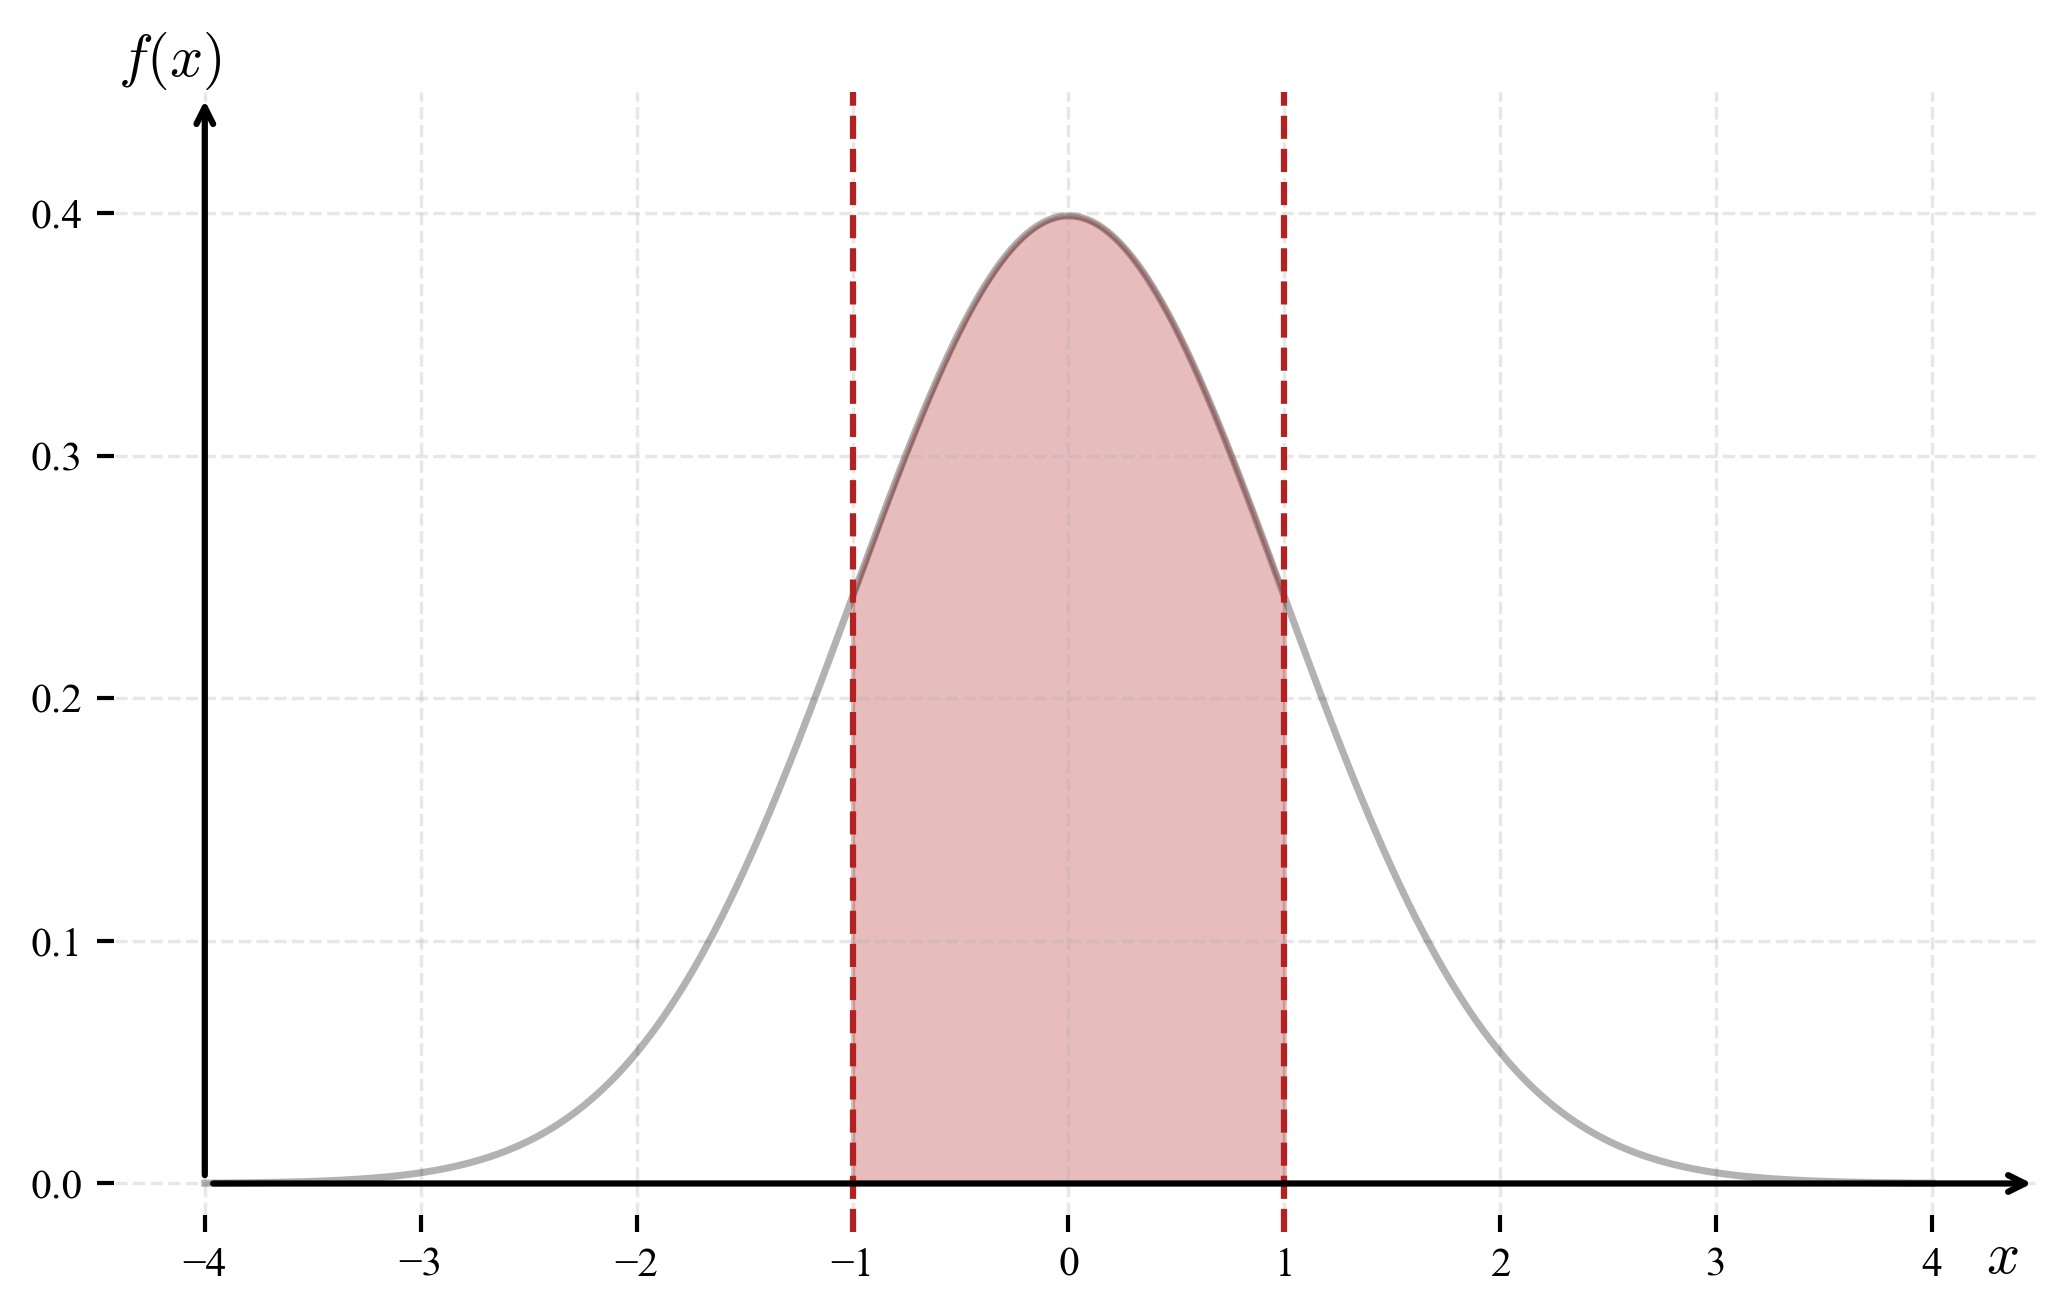
\includegraphics[width=0.7\textwidth]{figures/chapter2/gaussian_2.png}
    \caption{Representation of the law or large numbers. The sample mean tends to the population mean as the number of rolls $n$ increases.}
    \label{fig:random}
\end{figure}

\newpage

\section{The Central Limit Theorem}

The \textit{Central Limit Theorem} (CLT) is one of the most fundamental results of probability theory. It asserts that, under general conditions, the sum (or average) of a large number of independent random variables behaves approximately like a normally distributed variable, even if the original variables themselves are not normally distributed. This surprising and powerful result provides the mathematical explanation for the pervasive appearance of the bell-shaped curve in natural and social phenomena, and it serves as the theoretical backbone of most inferential statistics.

\medskip

The CLT emerges from the cumulative effect of many small, independent random influences. Imagine measuring something like the height of individuals, the result of which is shaped by many genetic, nutritional, and environmental factors. These influences may individually follow different distributions - some skewed, some bounded - but together, their additive or average effect tends to "smooth out" into a normal distribution. This smoothing occurs because the distribution of the sum is shaped by the convolution of the individual distributions, and repeated convolutions (under certain conditions) tend to produce a Gaussian shape—a phenomenon akin to a probabilistic version of the law of large numbers.

\medskip

The intuitive reason for this is rooted in the \textit{independence} of the variables and the \textit{averaging effect} of the sum. Each random variable contributes a little "noise" to the final result, and the accumulation of many such noises results in a distribution that reflects the most probable outcome: symmetrically clustered around the mean, with tails governed by how much variability the individual sources introduce.

\medskip

The first instance of a central limit-like result appears in the work of Abraham de Moivre in 1733, who demonstrated that the binomial distribution could be approximated by the normal distribution under certain conditions. Then Laplace extended this in 1810 to more general discrete distributions. These early forms assumed identically distributed, bounded, and often symmetric variables.

\begin{figure}[ht]
    \centering
    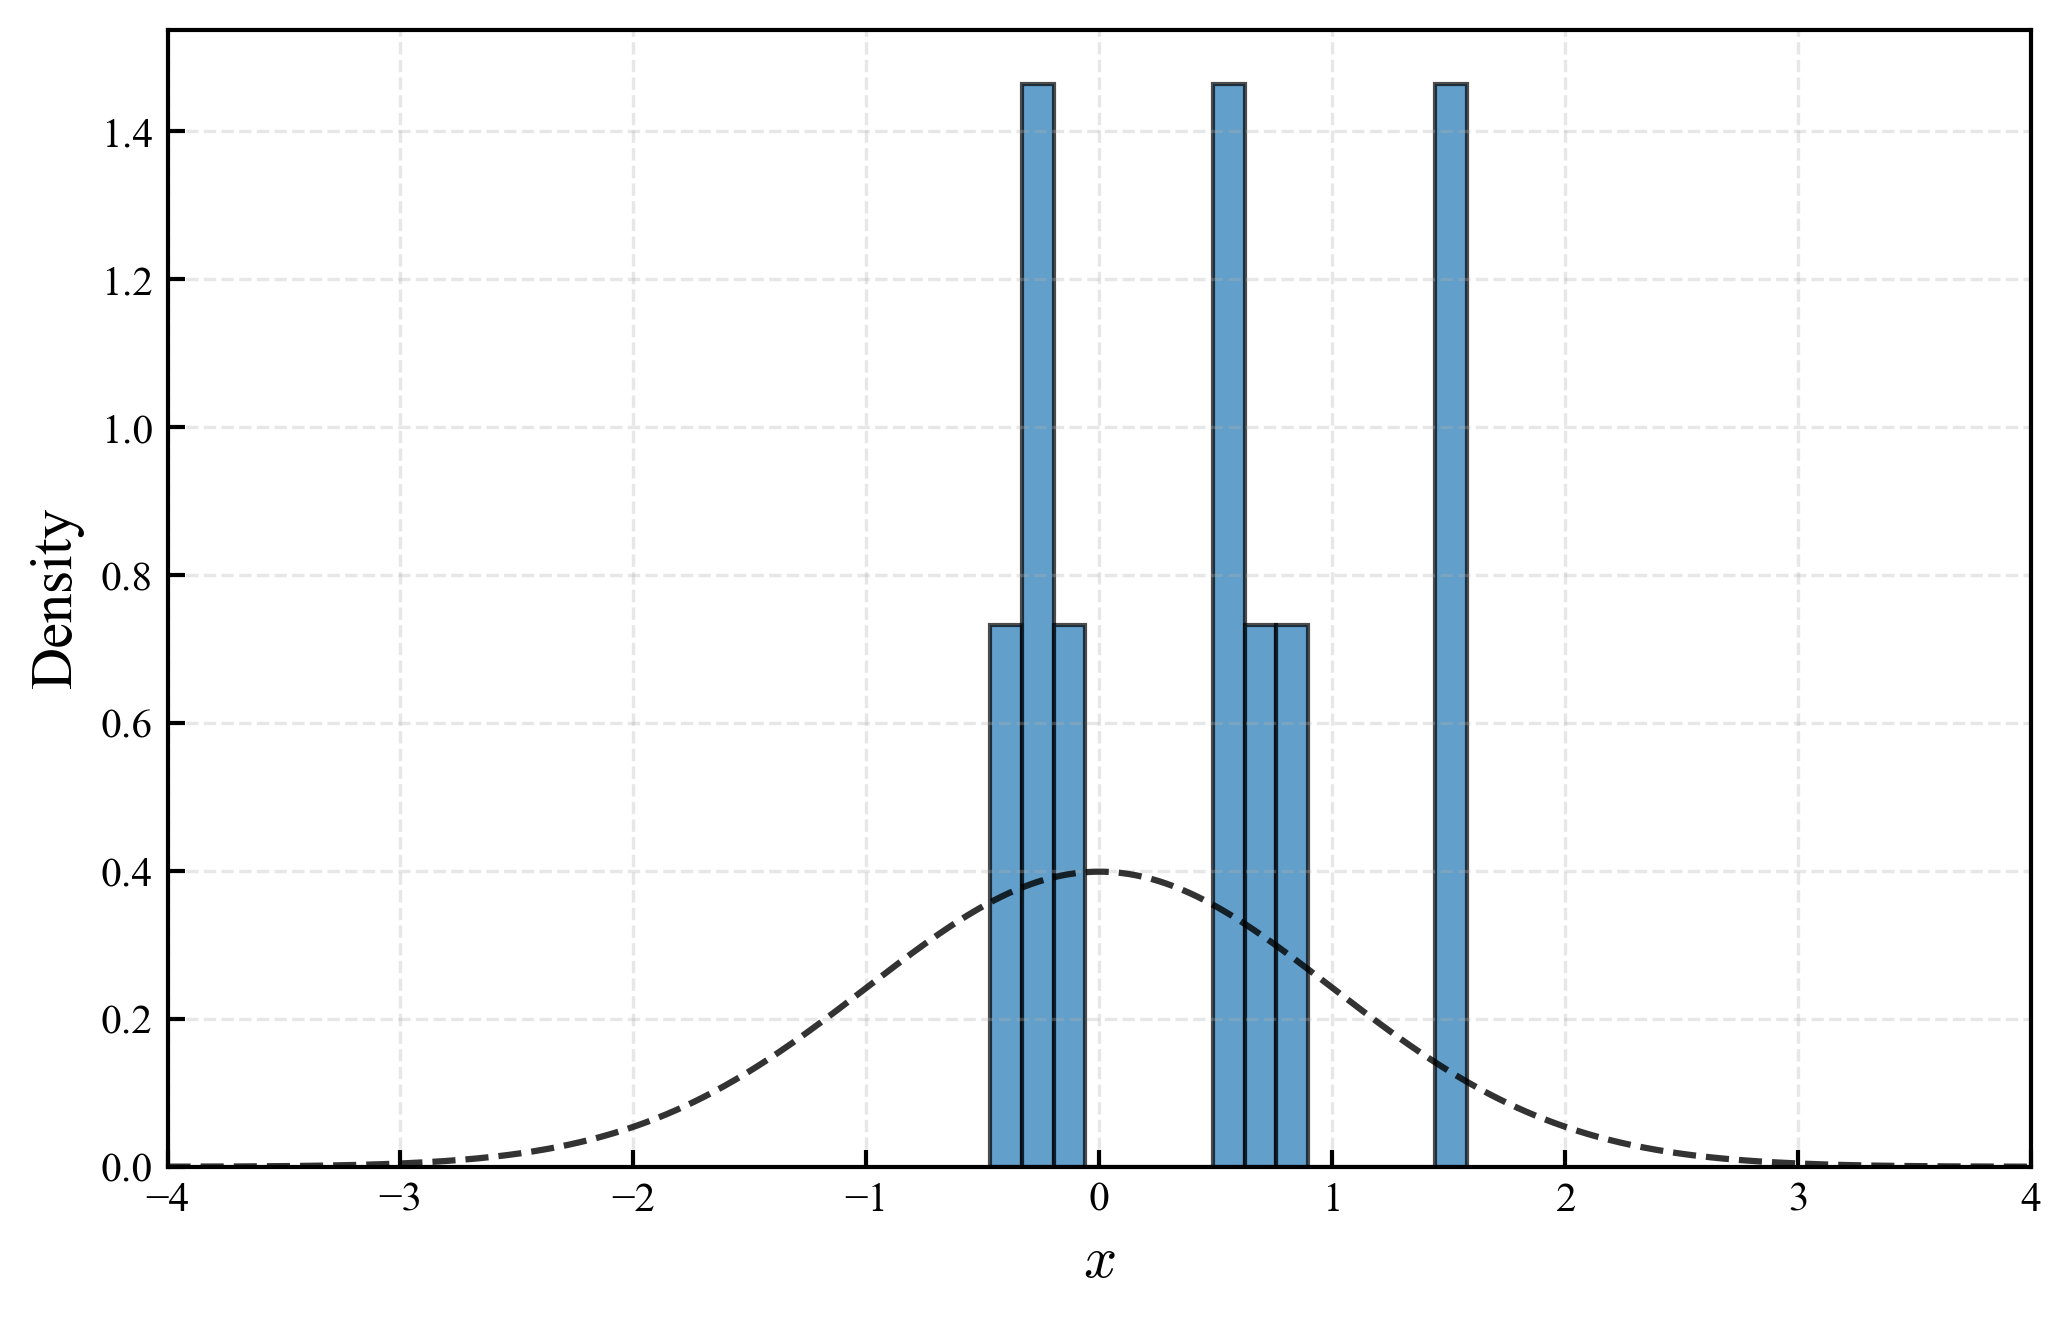
\includegraphics[width=0.6\textwidth]{figures/chapter3/clt_1.png}
    \caption{Histogram representing a set of observations and the central limit theorem. The sample mean follows a gaussian distribution as the sample size $n$ increases.}
    \label{fig:random}
\end{figure}

A more general and rigorous version came from Russian mathematician Aleksandr Lyapunov in 1901, who removed many of these restrictions and provided a sufficient condition for convergence using higher-order moments. Later, J. W. Lindeberg refined the result further introducing the now-famous \textit{Lindeberg condition}, which allows for non-identically distributed variables and still guarantees convergence under the right circumstances.

Formal Statement (Classical Version): Let $x_1, x_2, \dots, x_n$ be a sequence of independent and identically distributed (i.i.d.) random variables with some finite expected value $\mu = \mathbb{E}[X_i]$ and finite, positive variance $\sigma^2 = \operatorname{Var}(X_i)$. We can define the sample mean as we did in previous section:

\begin{equation}
	\overline{x}_n = \frac{1}{n} \sum_{i=1}^n x_i.
\end{equation}

Then the Central Limit Theorem (in its classical form, as due to Lyapunov, 1901) states that the distribution of the \textit{normalized} - or \textit{standardized} - sample mean

\begin{equation}
	Z_n = \frac{\sqrt{n}(\overline{X}_n - \mu)}{\sigma}
\end{equation}

converges to the standard normal distribution $\mathcal{N}(0,1)$ as $n \to \infty$. That is,

\begin{equation}
	\lim_{n \to \infty} \mathbb{P}\left( \frac{\sqrt{n}(\overline{X}_n - \mu)}{\sigma} \leq z \right) = \Phi(z), \quad \text{for all } z \in \mathbb{R},
\end{equation}

where \( \Phi(z) \) is the cumulative distribution function of the standard normal distribution:

\begin{equation}
	\Phi(z) = \frac{1}{\sqrt{2\pi}} \int_{-\infty}^z e^{-t^2/2} \, dt.
\end{equation}

\begin{figure}[ht]
    \centering
    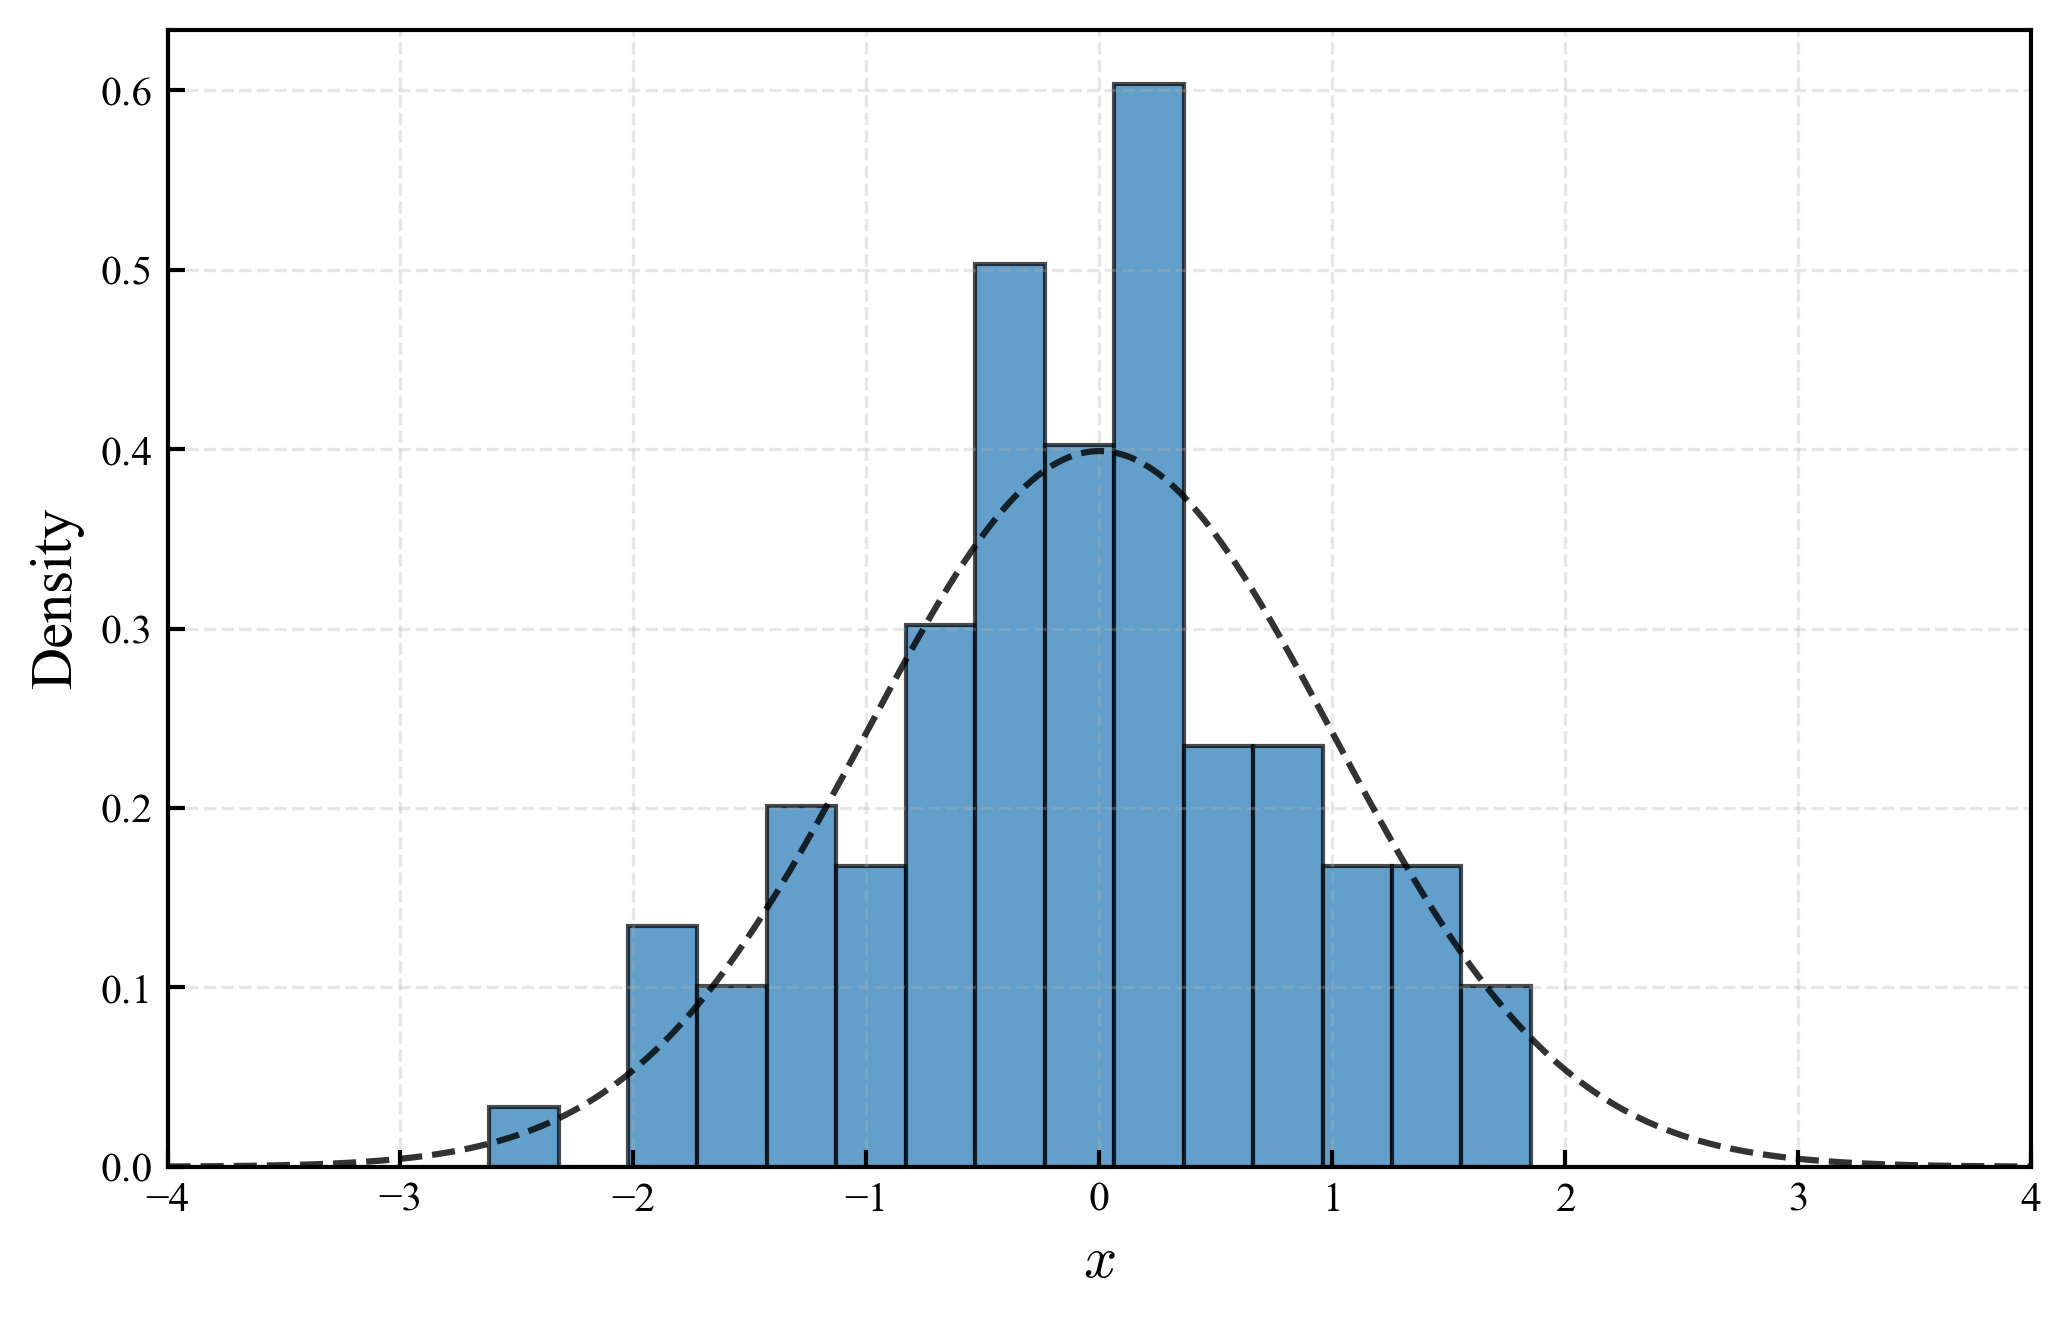
\includegraphics[width=0.6\textwidth]{figures/chapter3/clt_2.png}
    \caption{Histogram representing a set of observations and the central limit theorem. The sample mean follows a gaussian distribution as the sample size $n$ increases.}
    \label{fig:random}
\end{figure}

This form of convergence—called \textit{convergence in distribution} - means that the shape of the probability distribution of $Z_n$ approaches that of a standard normal variable as the sample size increases, regardless of the original distribution of the $X_i$, provided they are i.i.d. with finite mean and variance.

\medskip

\textbf{Example}

To illustrate the CLT in action, consider the following basic pen-and-paper experiment:

Let each \( X_i \) be a discrete uniform random variable on \( \{1, 2, 3, 4, 5, 6\} \), modeling a fair die roll. Then:

Compute expected, true mean value
\[
	\mu = \mathbb{E}[X_i] = \frac{1 + 2 + 3 + 4 + 5 + 6}{6} = 3.5,
\]

Compute variance operator
\[
	\sigma^2 = \operatorname{Var}(X_i) = \frac{1}{6} \sum_{k=1}^6 (k - 3.5)^2 = \frac{35}{12} \approx 2.9167.
\]

Now simulate \( n = 30 \) rolls, compute the sample mean \( \overline{X}_{30} \), and normalize:
\[
	Z_{30} = \frac{\sqrt{30}(\overline{X}_{30} - 3.5)}{\sqrt{35/12}}.
\]

Repeat this experiment several times (either with real dice or a random number generator). You will find that the histogram of the resulting \( Z_{30} \) values increasingly resembles the standard normal distribution. This is the Central Limit Theorem in action: even though each die roll is far from normally distributed (it’s discrete and uniform), the average of many such rolls behaves approximately normally.

\medskip

Conclusion, the Central Limit Theorem provides a bridge between the randomness of individual observations and the predictability of averages. It explains why normality arises in so many empirical settings and justifies the widespread use of the normal distribution in statistical methods. As sample sizes grow, the shape of the distribution of sample means stabilizes around the normal curve—allowing us to invoke Gaussian models even in non-Gaussian worlds.

\begin{figure}[ht]
    \centering
    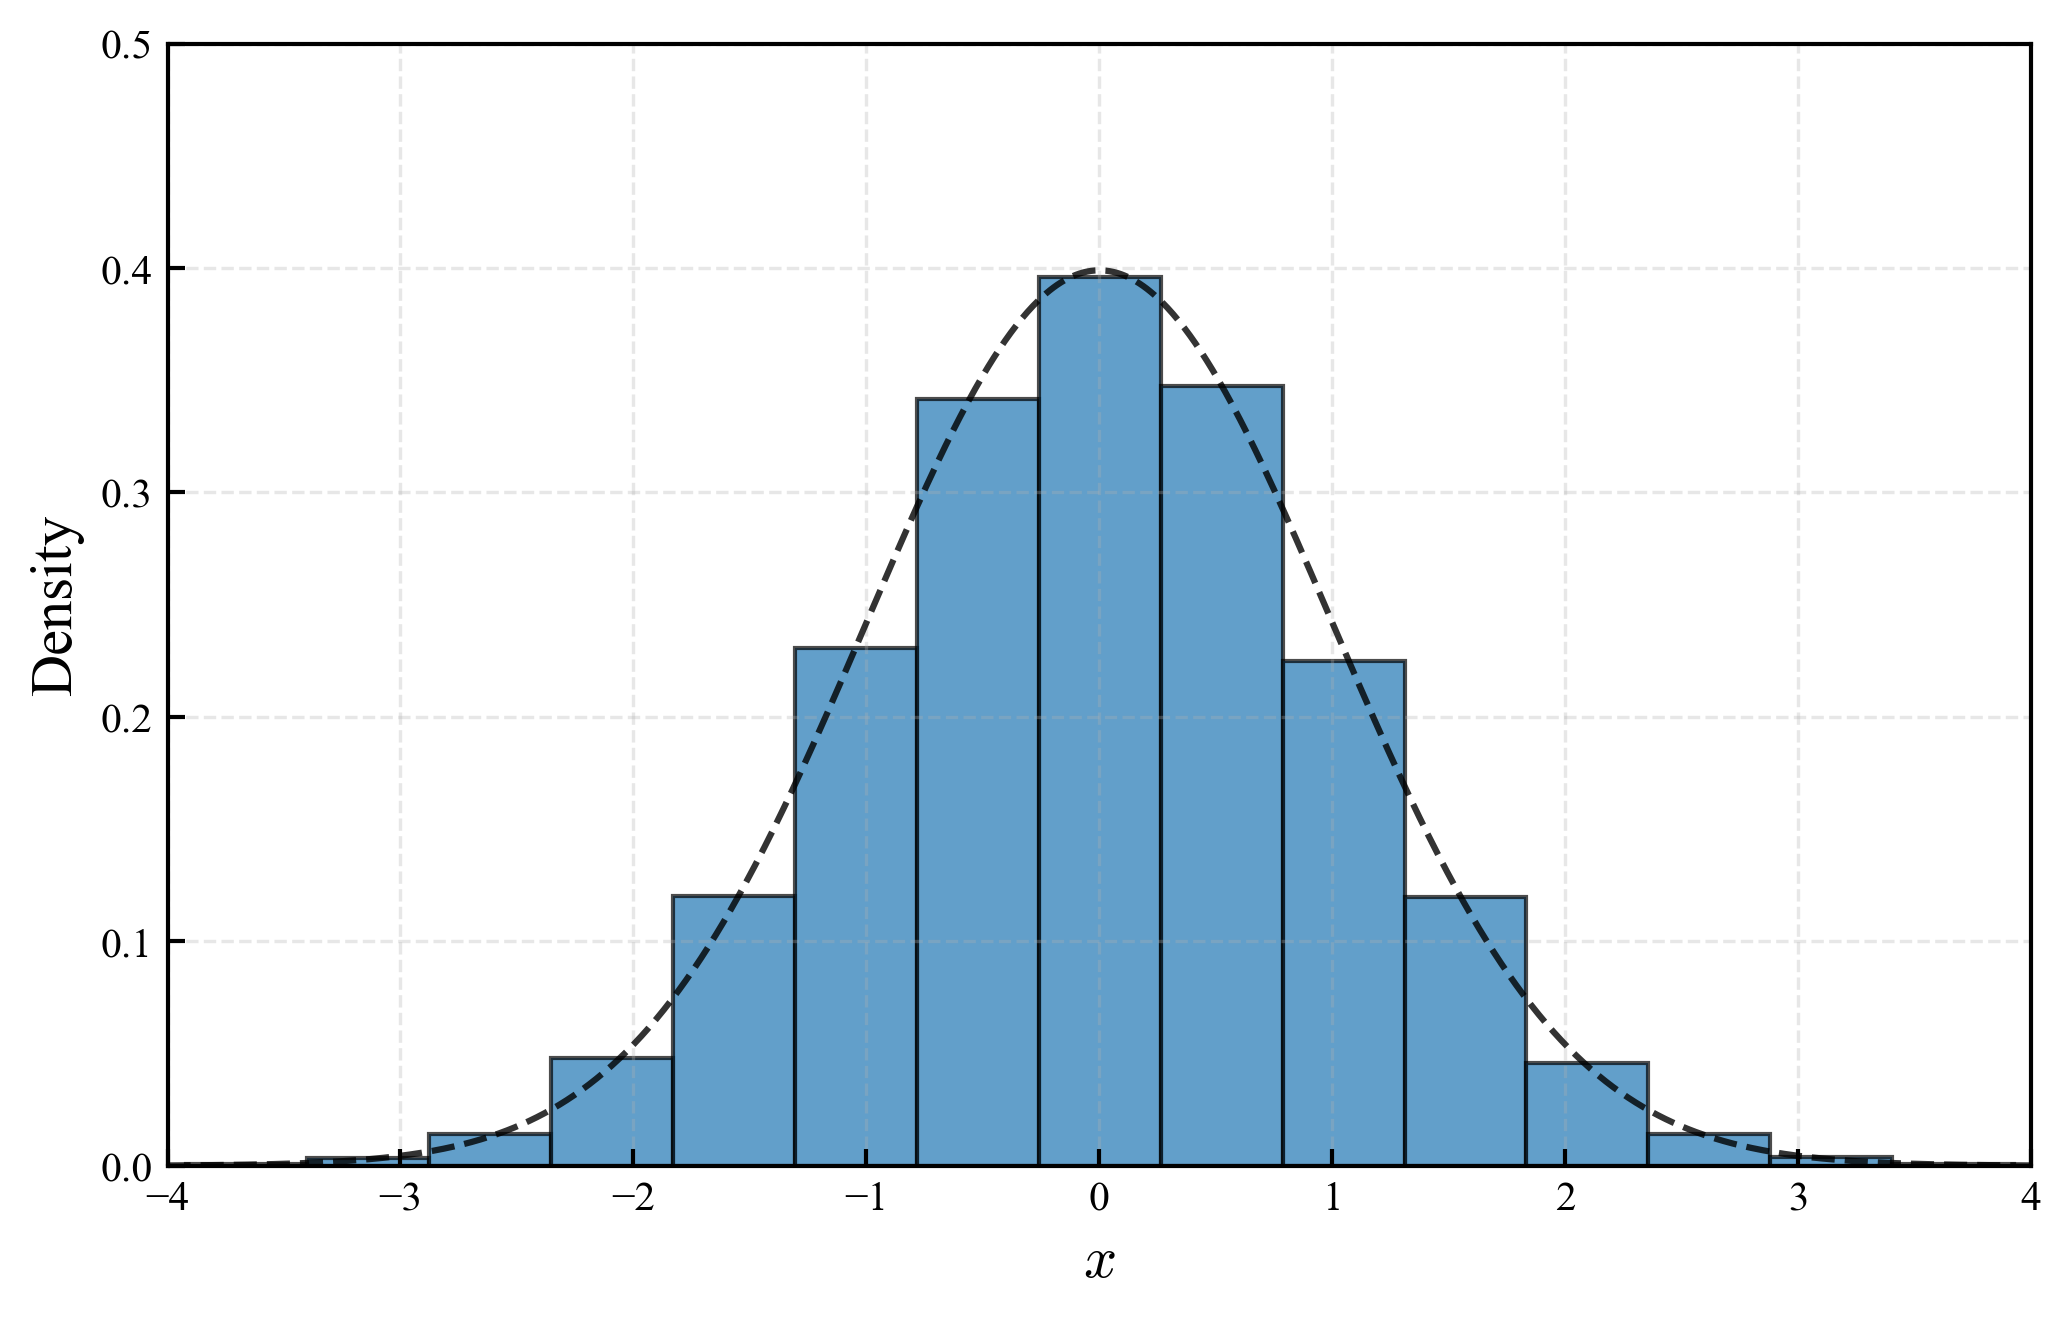
\includegraphics[width=0.6\textwidth]{figures/chapter3/clt_3.png}
    \caption{Histogram representing a set of observations and the central limit theorem. The sample mean follows a gaussian distribution as the sample size $n$ increases.}
    \label{fig:random}
\end{figure}

\newpage

\section{Maximum Likelihood Estimation}

\textbf{Maximum Likelihood Estimation} (MLE) is one of the most fundamental methods in statistical inference. It provides a systematic way to estimate unknown parameters of a statistical model by selecting the parameter values that make the observed data most probable. Conceptually intuitive and mathematically powerful, MLE serves as a unifying framework across many areas of statistics, from simple models to complex machine learning systems.

\subsection*{Motivation and Intuition}

Suppose we observe some data that we believe arises from a probabilistic model depending on unknown parameters. The central idea of MLE is to reverse the process: rather than asking “what data might result from given parameters?”, we ask “which parameters are most likely to have generated the data we actually observed?”

More formally, we treat the likelihood—the probability (or probability density) of the observed data given a parameter—as a function of the parameter. We then choose the value of the parameter that maximizes this function. This value is called the \emph{maximum likelihood estimate}.

This approach aligns with our everyday reasoning: if you observe a coin come up heads 90 out of 100 times, the parameter value (e.g., probability of heads) that best explains this data is likely around 0.9, not 0.5.

\subsection*{Historical Background}

The method of maximum likelihood was introduced by \textbf{Ronald A. Fisher} in a series of seminal papers beginning in 1912 and formally developed in 1922. Fisher championed likelihood as a key concept in statistical inference, distinguishing it from Bayesian methods and providing it with a firm theoretical foundation. He also showed that under regularity conditions, MLEs are consistent, asymptotically normal, and efficient—properties that make them highly desirable estimators.

\subsection*{Formal Definition}

Let \( X_1, X_2, \dots, X_n \) be a random sample from a distribution with probability density function (pdf) or probability mass function (pmf) \( f(x; \theta) \), where \( \theta \in \Theta \subseteq \mathbb{R}^k \) is the (possibly multivariate) parameter to be estimated.

The \textbf{likelihood function} is defined as:

\[
L(\theta; x_1, \dots, x_n) = \prod_{i=1}^n f(x_i; \theta),
\]

viewed as a function of \( \theta \), with the observed data \( x_1, \dots, x_n \) held fixed.

The \textbf{maximum likelihood estimator} (MLE) \( \hat{\theta}_{\text{MLE}} \) is the value of \( \theta \) that maximizes this likelihood function:

\[
\hat{\theta}_{\text{MLE}} = \arg\max_{\theta \in \Theta} L(\theta; x_1, \dots, x_n).
\]

Often it is more convenient to maximize the \textbf{log-likelihood function}, since the logarithm is a monotonic transformation and turns the product into a sum:

\[
\ell(\theta) = \log L(\theta; x_1, \dots, x_n) = \sum_{i=1}^n \log f(x_i; \theta).
\]

Then the MLE is equivalently given by:

\[
\hat{\theta}_{\text{MLE}} = \arg\max_{\theta \in \Theta} \ell(\theta).
\]

\subsection*{A Simple Example: Estimating a Bernoulli Parameter}

Suppose \( X_1, \dots, X_n \) are i.i.d. samples from a Bernoulli distribution with unknown parameter \( \theta \in [0,1] \), where:

\[
f(x; \theta) = \theta^x (1 - \theta)^{1 - x}, \quad x \in \{0, 1\}.
\]

Let the observed data be \( x_1, \dots, x_n \), with \( S = \sum_{i=1}^n x_i \) denoting the number of successes.

Then the likelihood function is:

\[
L(\theta) = \prod_{i=1}^n \theta^{x_i}(1 - \theta)^{1 - x_i} = \theta^S (1 - \theta)^{n - S}.
\]

The log-likelihood is:

\[
\ell(\theta) = S \log \theta + (n - S) \log(1 - \theta).
\]

To find the maximum, we differentiate and set to zero:

\[
\frac{d\ell}{d\theta} = \frac{S}{\theta} - \frac{n - S}{1 - \theta} = 0.
\]

Solving:

\[
\frac{S}{\theta} = \frac{n - S}{1 - \theta} \quad \Rightarrow \quad \hat{\theta}_{\text{MLE}} = \frac{S}{n}.
\]

Thus, the MLE of \( \theta \) is the sample mean: the proportion of successes. This simple example highlights the natural interpretation of MLE: it finds the parameter that best matches the empirical data.

\subsection*{Asymptotic Properties}

Under regularity conditions, the MLE enjoys desirable asymptotic properties:

\begin{itemize}
  \item \textbf{Consistency:} \( \hat{\theta}_{\text{MLE}} \to \theta \) in probability as \( n \to \infty \).
  \item \textbf{Asymptotic Normality:} \( \sqrt{n}(\hat{\theta}_{\text{MLE}} - \theta) \overset{d}{\to} \mathcal{N}(0, I(\theta)^{-1}) \), where \( I(\theta) \) is the Fisher information.
  \item \textbf{Asymptotic Efficiency:} The MLE achieves the Cramér-Rao lower bound asymptotically.
\end{itemize}

\subsection*{Conclusion}

Maximum Likelihood Estimation offers a principled and widely applicable method for estimating parameters in statistical models. It connects theory with practice: given data and a model, MLE identifies the parameter values that render the observed data most plausible. Its generality, consistency, and strong asymptotic properties make it a cornerstone of classical statistics and a workhorse of modern machine learning.

\newpage

\paragraph{Historical Context:}
Maximum Likelihood Estimation was introduced by the statistician Ronald Fisher in the early 20th century. Fisher’s key insight was that many statistical problems can be solved by choosing the parameters of a model that make the observed data most probable. This approach unified estimation methods and became one of the most fundamental tools in statistics. MLE connects well with probability theory and has wide applications, from genetics to machine learning.

\paragraph{Why Maximum Likelihood?}
In statistics, we often have data generated by some unknown process described by parameters. The goal of MLE is to find the parameter values that best explain the observed data. By defining a likelihood function (the probability of observing the data given parameters), MLE picks the parameters that maximize this function, thus providing the most “likely” explanation.

\paragraph{Applications of MLE:}
MLE is widely used because it produces estimates with good theoretical properties: under mild conditions, MLE estimators are consistent (they get closer to the true value as data grows) and efficient (they have the smallest possible variance among unbiased estimators). It forms the backbone of many models and is implemented in most statistical software.\\

Maximum Likelihood Estimation (MLE) is a cornerstone of modern statistical inference. Developed in the early 20th century by Sir Ronald A. Fisher, MLE provides a systematic framework for estimating the parameters of a probabilistic model. Fisher introduced the method in the 1920s, formalizing it as a rigorous alternative to the method of moments and laying the groundwork for much of classical and modern statistical theory.
MLE has since become one of the most widely used estimation techniques due to its generality, mathematical tractability, and strong theoretical properties. It applies to a broad class of models, including both discrete and continuous distributions, and serves as the basis for many advanced statistical methods, including Generalized Linear Models (GLMs), Bayesian inference (as the likelihood term), and machine learning algorithms.

\subsection{Motivation and intuition}
MLE seeks the parameter $\theta$ that makes the observed data most probable under the assumed model. In other words, it chooses the parameter that maximizes the likelihood function:

\[
L(\theta) = P(X_1 = x_1, \dots, X_n = x_n \mid \theta)
\]

\textbf{Example:} For a Bernoulli distribution with unknown probability $p$, the likelihood of observing a sequence of 0s and 1s is:

\[
L(p) = \prod_{i=1}^{n} p^{x_i}(1-p)^{1 - x_i}
\]

\subsection{The Likelihood and Log-Likelihood functions}

For independent and identically distributed data $X_1, \dots, X_n$ with density or mass function $f(x; \theta)$, the likelihood function is:

\[
L(\theta) = \prod_{i=1}^{n} f(x_i; \theta)
\]

To simplify differentiation, we often use the \textbf{log-likelihood}:

\[
\ell(\theta) = \log L(\theta) = \sum_{i=1}^{n} \log f(x_i; \theta)
\]

To find the MLE $\hat{\theta}$:

\begin{enumerate}
    \item Write down the log-likelihood $\ell(\theta)$.
    \item Take the derivative with respect to $\theta$: $\frac{d\ell}{d\theta}$.
    \item Solve $\frac{d\ell}{d\theta} = 0$ to find critical points.
    \item Check which value maximizes the likelihood (often via the second derivative or boundary checks).
\end{enumerate}

\textbf{Example: Bernoulli MLE}

For $X_i \sim \text{Bernoulli}(p)$,

\[
\ell(p) = \sum_{i=1}^{n} \left[x_i \log(p) + (1 - x_i)\log(1 - p)\right]
\]

Taking derivative:

\[
\frac{d\ell}{dp} = \sum_{i=1}^{n} \left[\frac{x_i}{p} - \frac{1 - x_i}{1 - p}\right] = \frac{\sum x_i}{p} - \frac{n - \sum x_i}{1 - p}
\]

Solving yields:

\[
\hat{p} = \frac{1}{n} \sum_{i=1}^{n} x_i
\]

\textbf{Properties of the MLE}

The importance of MLE lies not only in its general applicability but also in its powerful theoretical properties. 
Under regularity conditions, MLEs are asymptotically optimal estimators in the sense that they:
\begin{itemize}
\item \textbf{Consistency:} $\hat{\theta} \to \theta$ as $n \to \infty$
\item \textbf{Asymptotic Normality:} $\sqrt{n}(\hat{\theta} - \theta) \xrightarrow{d} \mathcal{N}(0, I(\theta)^{-1})$, where $I(\theta)$ is the Fisher information
\item \textbf{Efficiency:} Asymptotically achieves the Cram'er-Rao lower bound
\item \textbf{Invariance:} If $\hat{\theta}$ is the MLE of $\theta$, then $g(\hat{\theta})$ is the MLE of $g(\theta)$ for any differentiable function $g$
\end{itemize}
These properties make MLE a preferred method in both theoretical and applied statistics, especially for large-sample inference. 
In practice, these properties justify the use of MLE even when exact finite-sample distributions are hard to derive.

\textbf{Application to Generalized Linear Models}

Generalized Linear Models (GLMs) are an important class of models that extend linear regression to non-normal response variables by using a link function and a distribution from the exponential family. MLE plays a central role in fitting GLMs because the estimation of the model parameters is achieved by maximizing the likelihood of the observed responses.
For instance, in logistic regression---used for binary outcomes---the log-odds of success is modelled as a linear combination of predictors:\\

\textbf{Example: Logistic Regression}

For binary response data, logistic regression models the log-odds as a linear function of predictors:

\[
\log\left( \frac{p}{1 - p} \right) = \beta_0 + \beta_1 x
\]

MLE is used to estimate the coefficients $\beta_0, \beta_1$ by maximizing the binomial log-likelihood.

\newpage

\subsection*{Exercises}

\textbf{1.} Exercise [...].\\

\textbf{2.} Exercise [...].\\

\textbf{3.} Exercise [...].\\

\newpage

\subsection*{Solutions}

\textbf{1.} Solution [...].\\

\textbf{2.} Solution [...].\\

\textbf{3.} Solution [...].\\



% Chapter - Introduction to hypothesis testing .........................................................................................................................................................
\chapter{Introduction to hypothesis testing}

\epigraph{\textit{The object of statistical science is the reduction of data to relevant information.}}{— Ronald A. Fisher}

\section{Prediction vs inference}

In the previous chapters we have introduced the mathematical theory of probability. That is, we have developed a series of tools, a \textit{theory}, which enables us to make predictions about stochastic processes. But, contrary to what is normally explained in introductory courses, science is not always headed in the \textit{mathematical prediction followed by experimental measurement} direction. There are many cases, as we will soon see, where expectations - or \textit{hypothesis} are formulated for some given phenomena, and no prediction is made. In such cases, where we focus on interpretability rather than forecast, it is from measurement that we will try to see, or \textit{infer} if our hypothesis are compatible with given data. Indeed, most modern data analysis and hypothesis testing lie in the inferential statistics, rather than predictive probability \cite{fisher1925},  \cite{fisher1935}.\\

The philosophical division between prediction and inference has deep roots in the evolution of scientific reasoning. On the one hand we find prediction, which is more agnostic to explanation and utilitarian, ultimately concerned with \textit{what will happen next}. Inference, in contrast, is rooted in classical traditions of epistemology and induction, and seeks to illuminate the underlying structure or cause of observed data. It asks, fundamentally, \textit{why we see what we do}, invoking theories, latent mechanisms, and parameters that might explain the observed phenomena.\\

\begin{figure}[ht]
    \centering
    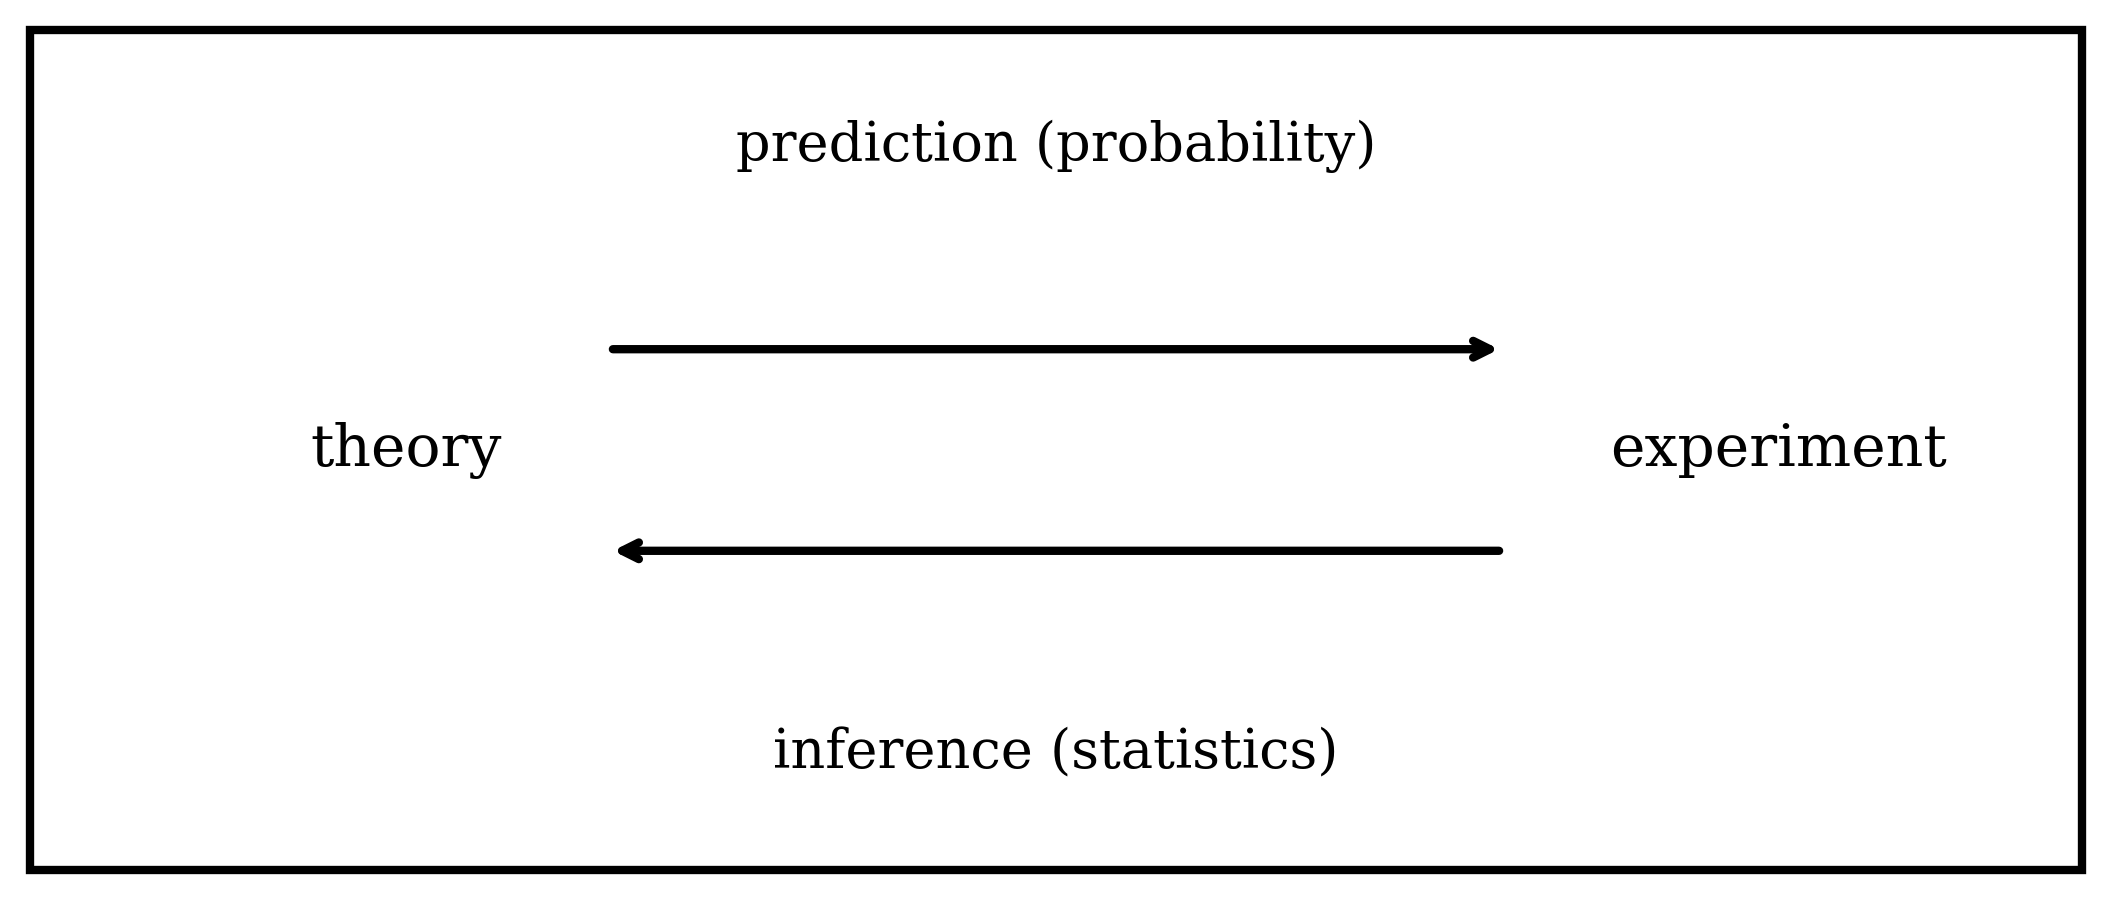
\includegraphics[width=0.6\textwidth]{figures/chapter4/probability_vs_statistics.png}
    \caption{Representation of the predictive (from theory to experimental verification) and inferential (from data to underlying truth, descriptive and hypothesis testing) approaches to probability and statistics \cite{pearson1900}.}
    \label{fig:prob_vs_stats1}
\end{figure}

Consider the examples we saw in previous chapters: there we developed a series of mathematical tools, algorithmic-wise, that enabled us to make predictions for the so-called Bernoulli, Binomial, Gaussian, ..., distributed events. For a random variable such as the face of the coin, or dice, or any other stochastic event we could measure in a laboratory, we built \textit{probability as a theory to predict} what would happen next, without going much deeper on why a certain set of events are Binomial, or Poisson, or Gaussian distributed, or why they follow these specific mathematical expressions.\\

This distinction becomes particularly important in statistical modeling. Predictive models, such as those deployed in machine learning, are often evaluated by their performance on unseen data, with little regard for the interpretability of parameters. Inference, however, thrives on interpretable structure — effect sizes, confidence intervals, causal assumptions — offering insights that extend beyond mere forecasting. Yet the two are not mutually exclusive: many contemporary methods, especially in Bayesian statistics, attempt to harmonize prediction and inference within unified frameworks. Still, when decisions hinge on understanding causation or evaluating mechanisms—as in medicine, economics, or the social sciences—inference retains a privileged role. We will review this topic in Chapter 6, when we focus on the Bayesian and frequentist definition of probability. Approaching modern times, the rise of probabilistic models in the 20\textsuperscript{th} century has made now possible to quantify uncertainty in both directions, but their goals remain distinct. Inference aims to learn about the data-generated process, while prediction aims to accurately forecast future observations, regardless - at times - of the process's inner interpretability \cite{fisher1925}.\cite{pearson1900}.\\

Within this context, hypothesis testing emerges as a formal tool to carry out inference under uncertainty. Popularized in the early 20\textsuperscript{th} century by Karl Pearson and Ronald A. Fisher, and later formalized by Jerzy Neyman and Egon Pearson, hypothesis testing provides a structured way to assess whether observed data is consistent with a particular theoretical claim. At its core, and as we will see in the next section, the method tests a "null" hypothesis (typically representing chance or no effect) against an "alternative" (commonly representing an unexpected event). Given these assumptions, we will build \textit{estimator} quantities from data, such as sample means and variances, and combine them to compute \textit{informative quantities}, sometimes referred as \textit{statistics} or \textit{statistic tests}. Then, we will calculate the probability of observing some data as extreme as ours under the null expectation. While often misused or misinterpreted, hypothesis testing remains foundational in the sciences, offering a bridge between data and theory, between the probabilistic world of prediction and the explanatory realm of inference \cite{welch1947}.\\

[Lindley] Inference \\

The formulation that has served statistics well throughout this century is based on the data having, for each value of a parameter, a probability distribution. This accords with the idea that the uncertainty in the data needs to be described probabilistically. It is desired to learn something about the parameter from the data. Generally not every aspect of the parameter is of interest, so write it as ($\Theta, \alpha$) where we wish to learn about $\Theta$ with $\alpha$ as a nuisance, to use the technical term [...].


\section{Hypothesis, significance, p-values}

The term \textit{hypothesis testing} is normally used to refer a broad set of tools addressing parameter estimation, inference, and various exploratory analysis on random measurements and observations. In the last decades, expressions like hypothesis testing, hypothesis test, statistical inference - sometimes referred to as exploratory analysis - have gained popularity and become one of the standards in most experimental sciences, given the automatization of experiments and the large amounts of data available.\\

Once we have covered the idea of parameter estimation, sample distributions, and the idea of estimators, we will now formulate hypothesis on the \textit{population}, or true - \textit{unkwnown} - parameters, and then build \textit{statistic tests} to quantify how far - or close - are these hypothesized values from the \textit{sample}, observed, experimental, values. And finally, we will quantify how certain we are about the values obtained - how \textit{significant} they are - computing the \textit{p-value}, standing from Pearson value [...].\\ The general approach we will follow, regardless of the kind of question we are after and the observations made, can be summarized as follows:

\begin{itemize}
\item Formulate \textit{null} hypothesis $H_0$ and \textit{alternative} hypothesis $H_1$ about the \textit{true} - \textit{population} parameters, generally for the mean or variance, \textit{prior to experiment}.
\item Collect data, make observations, make measurements.
\item Compute \textit{estimators} and \textit{informative quantities} from our observed values, normally referred to as \textit{statistics}, or \textit{statistic tests}.
\item Compute p-value, the probability that \textit{we obtained a value at least as extreme as the one we obtained for our statistic test}.
\item Accept or reject the null hypothesis, based on the p-value, which quantifies how probable was to see this result.
\end{itemize}

Here we should pause for some time, and we must review some basic concepts about integration and probabilities, as we will try to build a \textit{mathematically accurate definition} of significance and the idea of p-value. The idea of p-value was developed by Pearson in the 1920s - indeed, p comes from no other than Pearson-value, and it was built already on the framework of estimator quantities and statistic tests.\\

Recall for a moment the idea of cumulative probability. Take some random variable with known distribution (e.g., the probability of obtaining 3 times heads in 10 tosses of a coin, which we know follows a Binomial distribution).
\begin{equation}
    P(x = x_0; n, k) = \binom{n}{x_0} p^x (1-p)^{n-x},
\end{equation}

And ask now what is the probability of obtaining \textit{more than} 3 times heads. We know that this is given by the cumulative probability, 
\begin{equation}
    P(x > x_0; n, k) = \sum_{x = x_0}^{x_n}\binom{n}{x_i} p^x (1-p)^{n-x},
\end{equation}

And the analogous in a continuous variable
\begin{equation}
    f(x > x_0) = \int_{x_0}^{\infty} \; f(x) dx \; .
\end{equation}

Now, with these concepts in mind, let's imagine a general, simple hypothesis testing scenario. We have some random variable $x$ following a gaussian distribution, and a hypothesized value $\mu$ for its true - or \textit{population} mean. As we saw in Chapter 3, we can make a set of measurements, and out of these compute an estimator, for instance, a sample mean $\bar{x}$. The real hypothesis testing problem is now to compare these two quantities, and somehow \textit{quantify} how similar - or different - they are. There are many ways of doing this, but one simple case is to compute just a difference between the two. 

\begin{equation}
	t = \frac{\bar{x} - \mu}{\sigma} \quad.
\end{equation}

This is normally called a $t$ statistic, or a $t$ \textit{statistic} test, which we will describe in detail in the next section. For now, just consider it a useful quantity representing how similar the true mean and the sample mean are to each other. Note that as $\mu$ tends to $\bar{x}$, the $t$ variable tends to zero.\\

It is now, once we have computed a statistic, an informative quantity from our data, that we can ask: what was the probability, given that first assumption about the true mean, that we obtain this particular result for the $t$ variable? Note that the $t$ variable is computed out of our estimator $\bar{x}$, which was computed out of our random observations. Hence, the $t$ variable, and any other statistic test we could have built - a Fisher, a $\chi2$, etc -  \textit{is a random variable as well}, and it will follow \textit{some} distribution.\\

Now, from our set of observations, we will obtain a specific value, $t_{obs}$, standing for \textit{observed} $t$. Then, the p-value is defined as the probability of obtaining a value \textit{at least as extreme} as the one we obtained for our statistic, given our hypothesized value for the true - or population - parameter. In other words, given the null hypothesis was true. The \textit{at least as extreme} part is what enables the cumulative distribution. \\

\begin{equation}
    p = P(t > t_{obs}) = \int_{t_{obs}}^{\infty} \; f(t) \; dt,
\end{equation}

For the computation of the numerical value we just need to know what is the probability density of the $t$ variable. This way, we are just left with solving a simple integral [...].

\newpage

\section{Statistical tests: some examples}

\subsection{Compare sample mean with hypothesized value - One sample t-test}

The t-test, a cornerstone of inferential statistics, emerged from practical necessity in the early 20th century, in no other than the world of brewing: William Sealy Gosset, a statistician employed by the Guinness Brewery in Dublin, devised the method to address the problem of making reliable inferences from small sample sizes - a common challenge in quality control. Because Guinness forbade its employees from publishing research, Gosset adopted the pseudonym “Student,” and the t-test entered the statistical canon as “Student’s t-test.” Far from being a mere curiosity, this test helped lay the foundation for modern statistical thinking, offering a systematic way to evaluate whether observed differences could be attributed to chance \cite{student1908}.\\

Contextually, the t-test emerged during a period of growing interest in the mathematical modeling of uncertainty. While the 19th century had seen the establishment of probability theory and the development of the normal distribution by figures like Gauss and Laplace, it was not until the early 20th century that statisticians began to address the problem of small samples and experimental variability. Gosset’s innovation came at a time when the rigour of scientific inquiry was undergoing a deep transformation; where laboratory science, agricultural experimentation, and industrial quality control all demanded more precise methods of inference. The t distribution, with its tails heavier than the normal distribution, conveniently modelled the added uncertainty inherent in small datasets, capturing the low confidence in inferences drawn from limited observations.\\

In the broader sweep of statistical development, the t-test exemplifies the bridging of theoretical elegance and empirical utility, making it feasible for practitioners across disciplines to assess hypotheses without the need for large-scale experimentation. Its adaptability, whether in comparing means between two groups or assessing paired observations, has ensured its enduring presence in the researcher’s toolkit. Over a century later, the t-test remains not merely a relic of an industrial past but a living method, still invoked in clinical trials, psychological studies, and countless scientific explorations, bearing with it both the legacy of its creator and the evolving rigour of modern analysis.\\

\begin{figure}[ht]
    \centering
    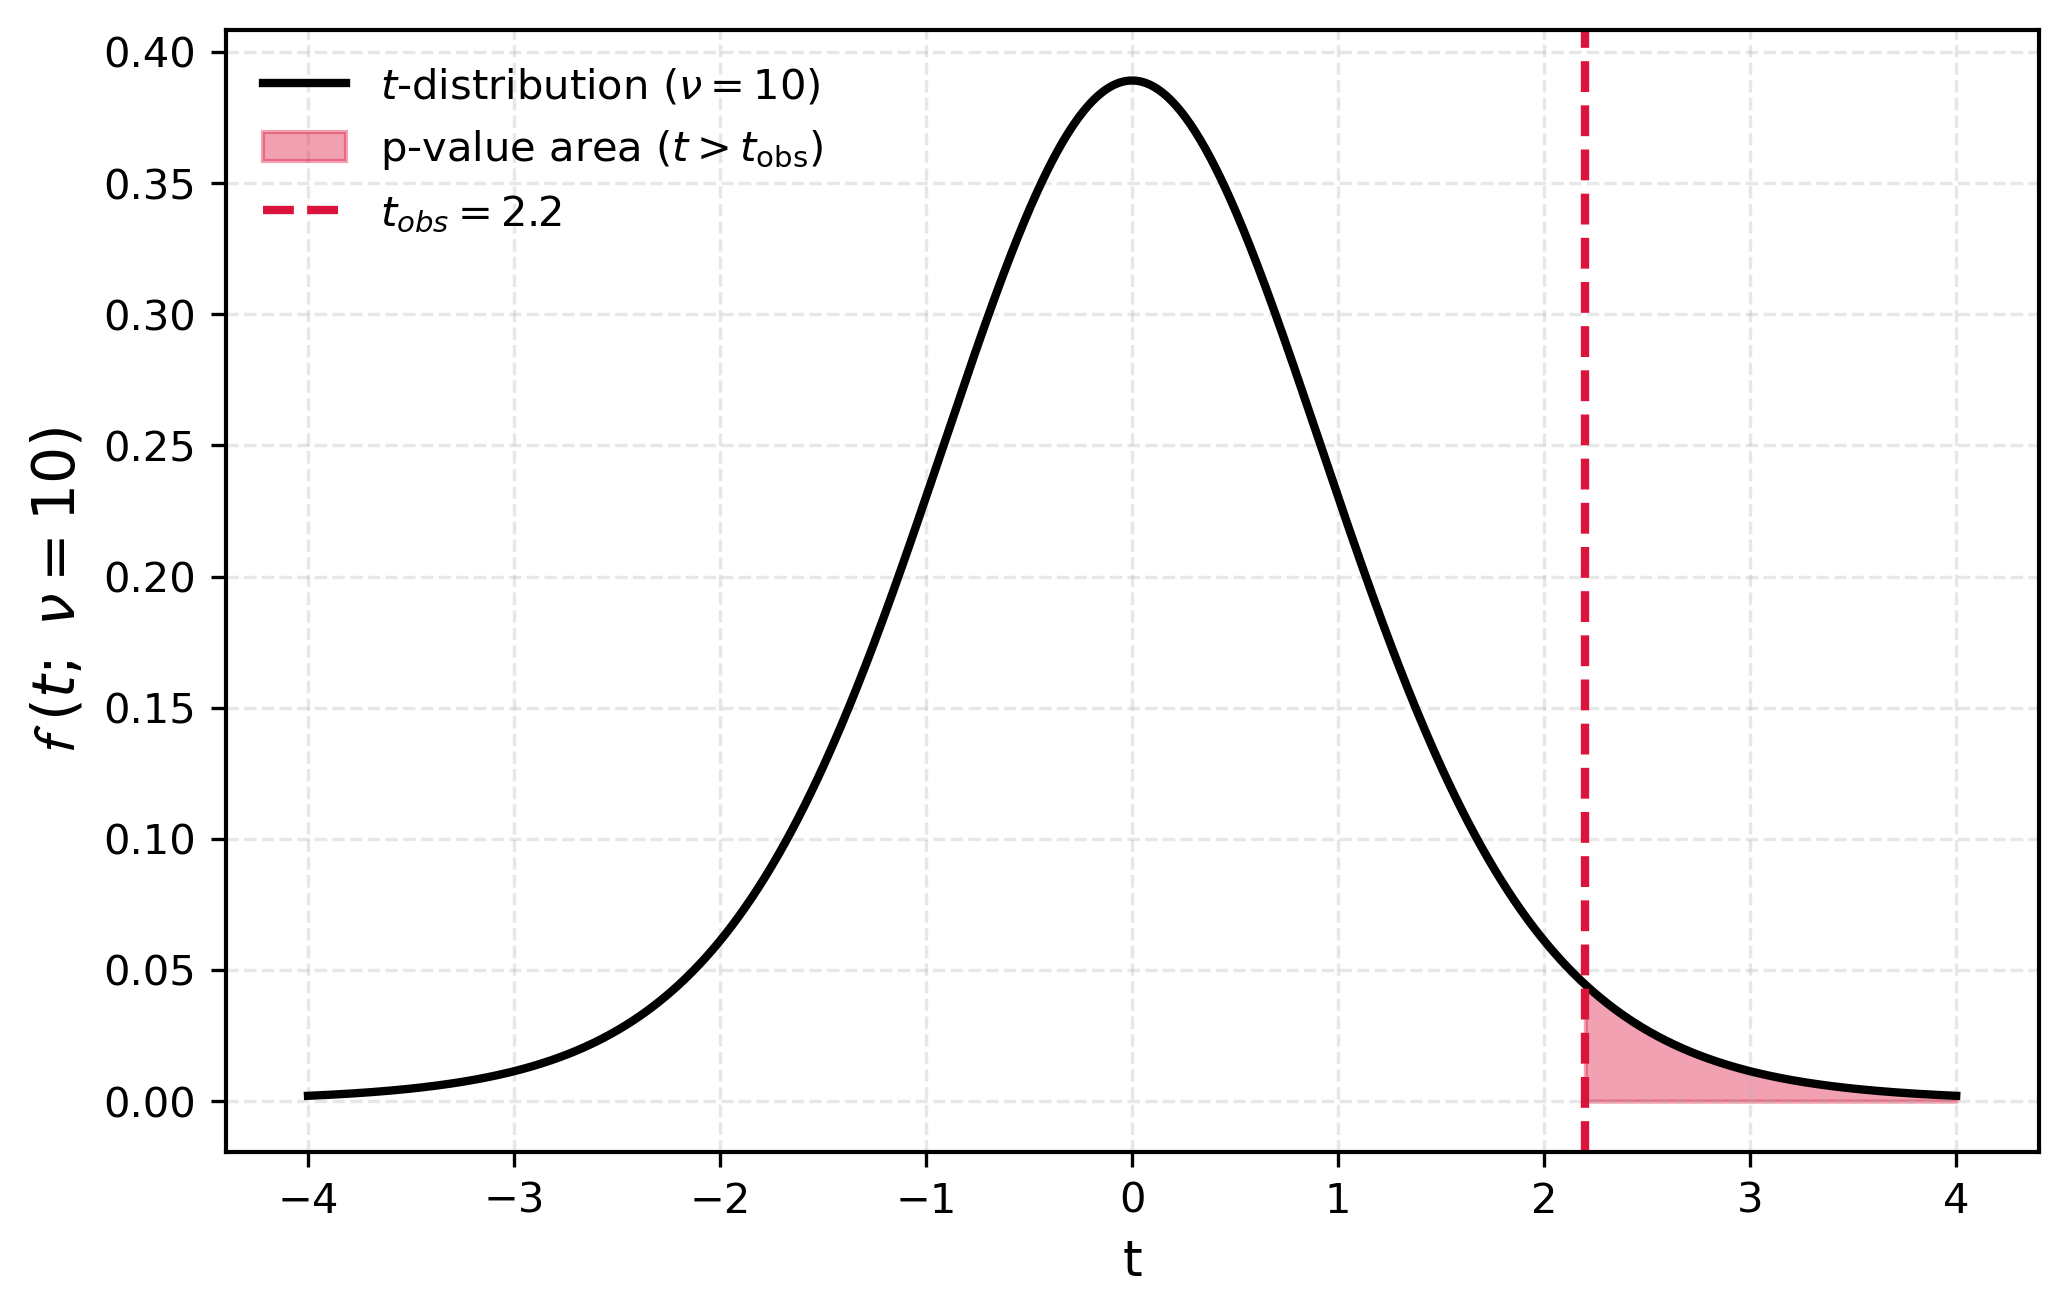
\includegraphics[width=0.7\textwidth]{figures/chapter4/t_test_1_sample_p_one_tailed.png}
    \caption{Representation of the t statistic, following the Student's t distribution, for a particular value of the degrees of freedom ($\nu = 10$). The integral of the shadowed area represents the \textit{1-sided}, or \textit{1-tailed} p-value, as the probability of obtaining a result \textit{at least as extreme} as the one obtained $t_{obs}$.}
    \label{fig:t_test1}
\end{figure}

The student's t is used to compare the sample mean $\bar{x}$ of a set of observations to ha hypothesized value $\mu$. It assumes that the sample data are drawn from a normally distributed population, hence it is an example of a \textit{parametric} test. We will discuss more about parametric and non-parametric observations, and how to test for normality further in the chapter. The t \textit{statistic test}, or t \textit{statistic}, or just t \textit{variable} for simplicity, is given by:
\begin{equation}
    t = \frac{\bar{x} - \mu}{s / \sqrt{n}},
\end{equation}

where $\bar{x}$ is the sample mean, $\mu$ is the population mean, $s$ is the sample standard deviation, and $n$ is the sample size. As we se, it is just a measure of how far the sample mean $\bar{x}$ and the hypothesized true value $\mu$ are from each other. Indeed, it is built in such a way that, as the sample mean $\bar{x}$ gets closer to the hypothesized value $\mu$, the $t$-variable approaches zero.\\

Then, given some data was observed and and we obtained a specific value for our t - let's call it \textit{$t_{obs}$}, to compute a p-value we just need to compute what was the probability of that particular value. To do that, we just recall our t variable was indeed a random variable depending on our random observations, which produced some random sample mean and variance, and some degrees of freedom $n - 1$
\begin{equation}
	p = P\left(t > t obs \right) = 2 \cdot \int_{|t|}^{\infty} f_{T_{n-1}}(x)\,dx = 2 \cdot \left[1 - F_{T_{n-1}}(|t|)\right]
\end{equation}

\subsection*{The t distribution}

Being $f_{T_{n-1}}$ the PDF of the t variable, the \textit{Student's t distribution} with $n - 1$ degrees of freedom, and $F_{T_{n-1}}$ the corresponding cumulative distribution, as we discussed in chapter 2 [...]. Here, we are computing the probability of t being greater than the one we obtained, and we do that just by integrating the t-distribution [...]. Note that here we are computing a 2-sided p-value, hence te factor 2 at the beginning.\\

Given a sample \( X_1, \ldots, X_n \sim \mathcal{N}(\mu, \sigma^2) \), the one-sample \textit{t}-statistic is defined as:
\[
t = \frac{\bar{X} - \mu_0}{S / \sqrt{n}}
\]
where \( \bar{X} \) is the sample mean, \( S \) is the sample standard deviation, and \( \mu_0 \) is the hypothesized population mean.

Under the null hypothesis \( H_0: \mu = \mu_0 \), the statistic follows a Student's \textit{t}-distribution with \( n-1 \) degrees of freedom:
\[
t \sim t_{n-1}
\]

The probability density function (PDF) of the \textit{t}-distribution with \( \nu \) degrees of freedom is:
\begin{equation}
	f(t; \; \nu) = \frac{\Gamma\left(\frac{\nu+1}{2}\right)}{\sqrt{\nu \pi} \, \Gamma\left(\frac{\nu}{2}\right)} \left(1 + \frac{t^2}{\nu}\right)^{-\frac{\nu+1}{2}}
\end{equation}
Distribution and computation of the p-value as defined above.

\newpage

\subsection{Compare sample means of two independent groups - Two sample t-test}

The two-sample t-test represents a natural extension of Gosset's original formulation, expanding its reach from single-sample inference to the comparison of two independent groups. This test seeks to determine whether the sample means, $\bar{x}_1$ and $\bar{x}_2$ of two populations are significantly different. It operates under the assumption that the underlying distributions are approximately normal and that the variances between groups are equal or at least comparable, though variants like Welch’s t-test have relaxed these conditions. The test statistic itself balances the observed difference in means against the pooled standard error, weighing signal against noise \cite{welch1947}.\\

The historical roots of the two-sample t-test are intertwined with the rise of controlled experimentation in the biological and social sciences during the early to mid-20th century. Ronald Fisher, Jerzy Neyman, and Egon Pearson contributed to formalizing the logic of hypothesis testing, and the t-test became a practical tool within this growing paradigm. Its popularity grew not merely because it was mathematically sound, but because it was accessible. A concise, simple and interpretable method for testing simple but essential questions in science: does treatment differ from control, is an observed effect more than a fluke, etc.\\

Even in today’s data-rich landscape, the two-sample t-test remains remarkably resilient. Its conceptual clarity and computational simplicity make it a first recourse in evaluating differences between two conditions, from clinical trials comparing drug efficacies to educational studies assessing learning interventions. In many ways, it is the distilled essence of statistical thinking: discerning pattern from randomness, while acknowledging uncertainty. Its elegance lies not in its complexity, but in its ability to render the ordinary rigorously meaningful.\\

\begin{figure}[ht]
    \centering
    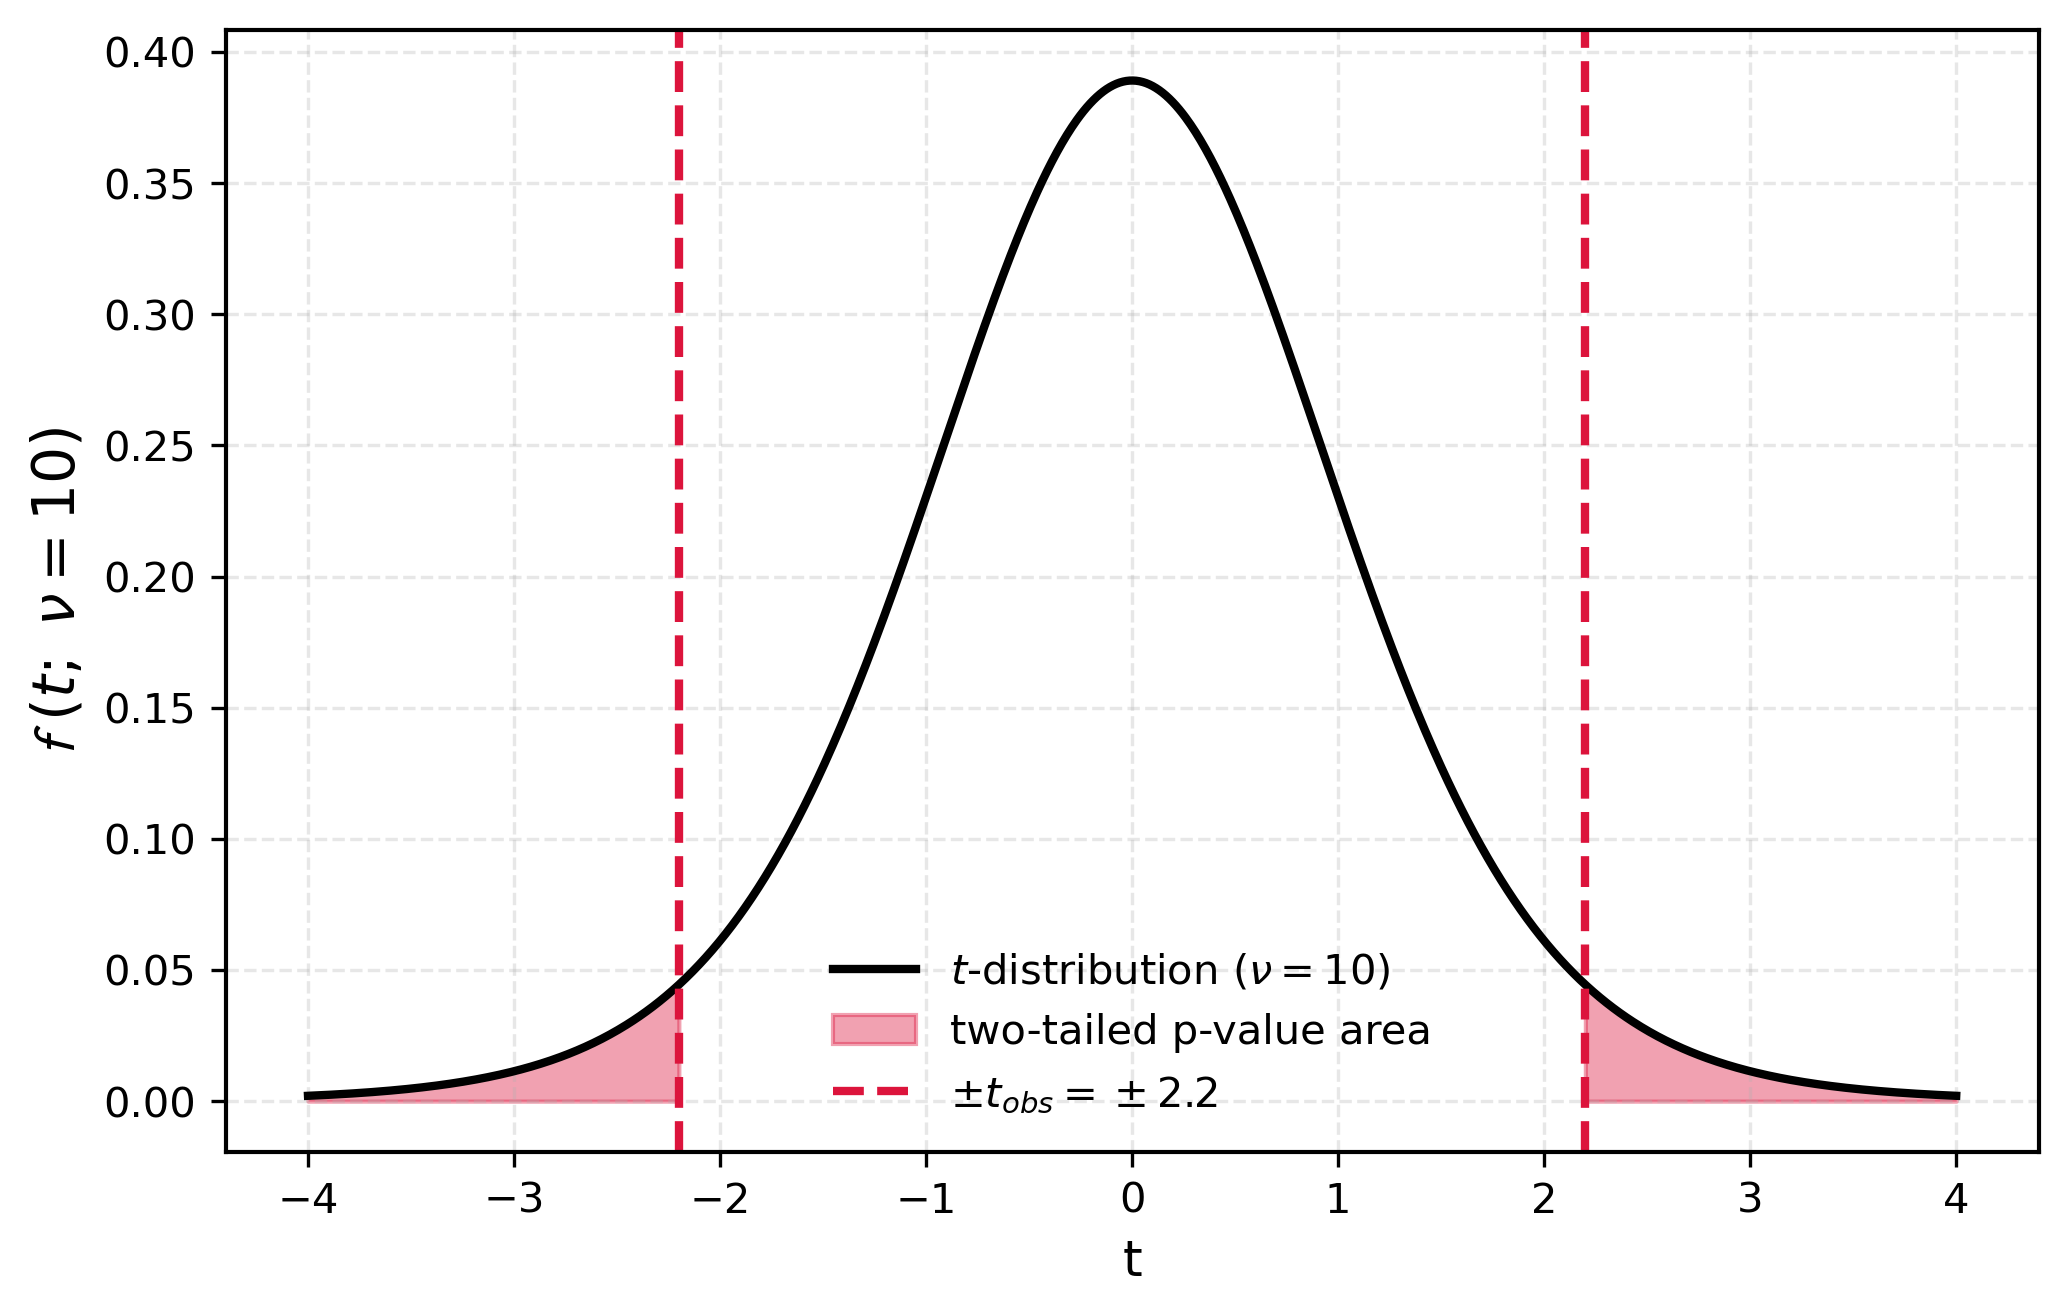
\includegraphics[width=0.7\textwidth]{figures/chapter4/t_test_1_sample_p_two_tailed.png}
    \caption{Representation of the t statistic, following the Student's t distribution, for a particular value of the degrees of freedom ($\nu = 10$). The integral of the shadowed area represents the \textit{2-sided}, or \textit{2-tailed} p-value, as the probability of obtaining a result \textit{at least as extreme} as the one obtained $t_{obs}$.}
    \label{fig:t_test2}
\end{figure}

The so-called \textit{two-sample t-test} is used to determine whether the sample means $\bar{x}_1$ and $\bar{x}_2$ of two sets of observations are significantly different from one another. It assumes that the sample data are drawn from a normally distributed population, hence it remains an example of parametric test. The t \textit{statistic test}, or t \textit{statistic}, or just t \textit{variable} for simplicity, is given by:
\begin{equation}
    t = \frac{\bar{x}_{1} - \bar{x}_{2}}{\sqrt{s^2_1 \big(n_{1} - 1)^{2} + s^2_2 (n_{2} - 1)^{2}}},
\end{equation}
where $\bar{x}_1$ and $\bar{x}_2$ are the sample means, $s^2_1$ and $s^2_2$ are the sample variances, $n_1$ and $n_2$ the sample sizes.\\

The computation of the p-value:
\begin{equation}
	p = P\left(t > t obs \right) = 2 \cdot \int_{|t|}^{\infty} f_{T_{df}}(x)\,dx = 2 \cdot \left[1 - F_{T_{df}}(|t|)\right]
\end{equation}

Being $f_{T_{n-1}}$ the PDF of the t variable, the \textit{Student's t distribution} with $n_1 + n_2 - 1$ degrees of freedom, and $F_{T_{n-1}}$ the corresponding cumulative distribution
Note here we assume equal variances. For Welch’s t-test (unequal variances), use the same form, but with Welch-adjusted [...]

\subsection*{The t distribution}

For two independent samples \( X_1, \ldots, X_n \sim \mathcal{N}(\mu_1, \sigma^2) \) and \( Y_1, \ldots, Y_m \sim \mathcal{N}(\mu_2, \sigma^2) \), the test statistic is:
\[
t = \frac{\bar{X} - \bar{Y}}{S_p \sqrt{\frac{1}{n} + \frac{1}{m}}}
\]
with pooled variance estimate:
\[
S_p^2 = \frac{(n-1)S_X^2 + (m-1)S_Y^2}{n + m - 2}
\]

Under \( H_0: \mu_1 = \mu_2 \), the statistic follows a \textit{t}-distribution with \( n + m - 2 \) degrees of freedom:
\[
t \sim t_{n+m-2}
\]
Distribution and computation of the p-value as defined above.

\begin{figure}[ht]
    \centering
    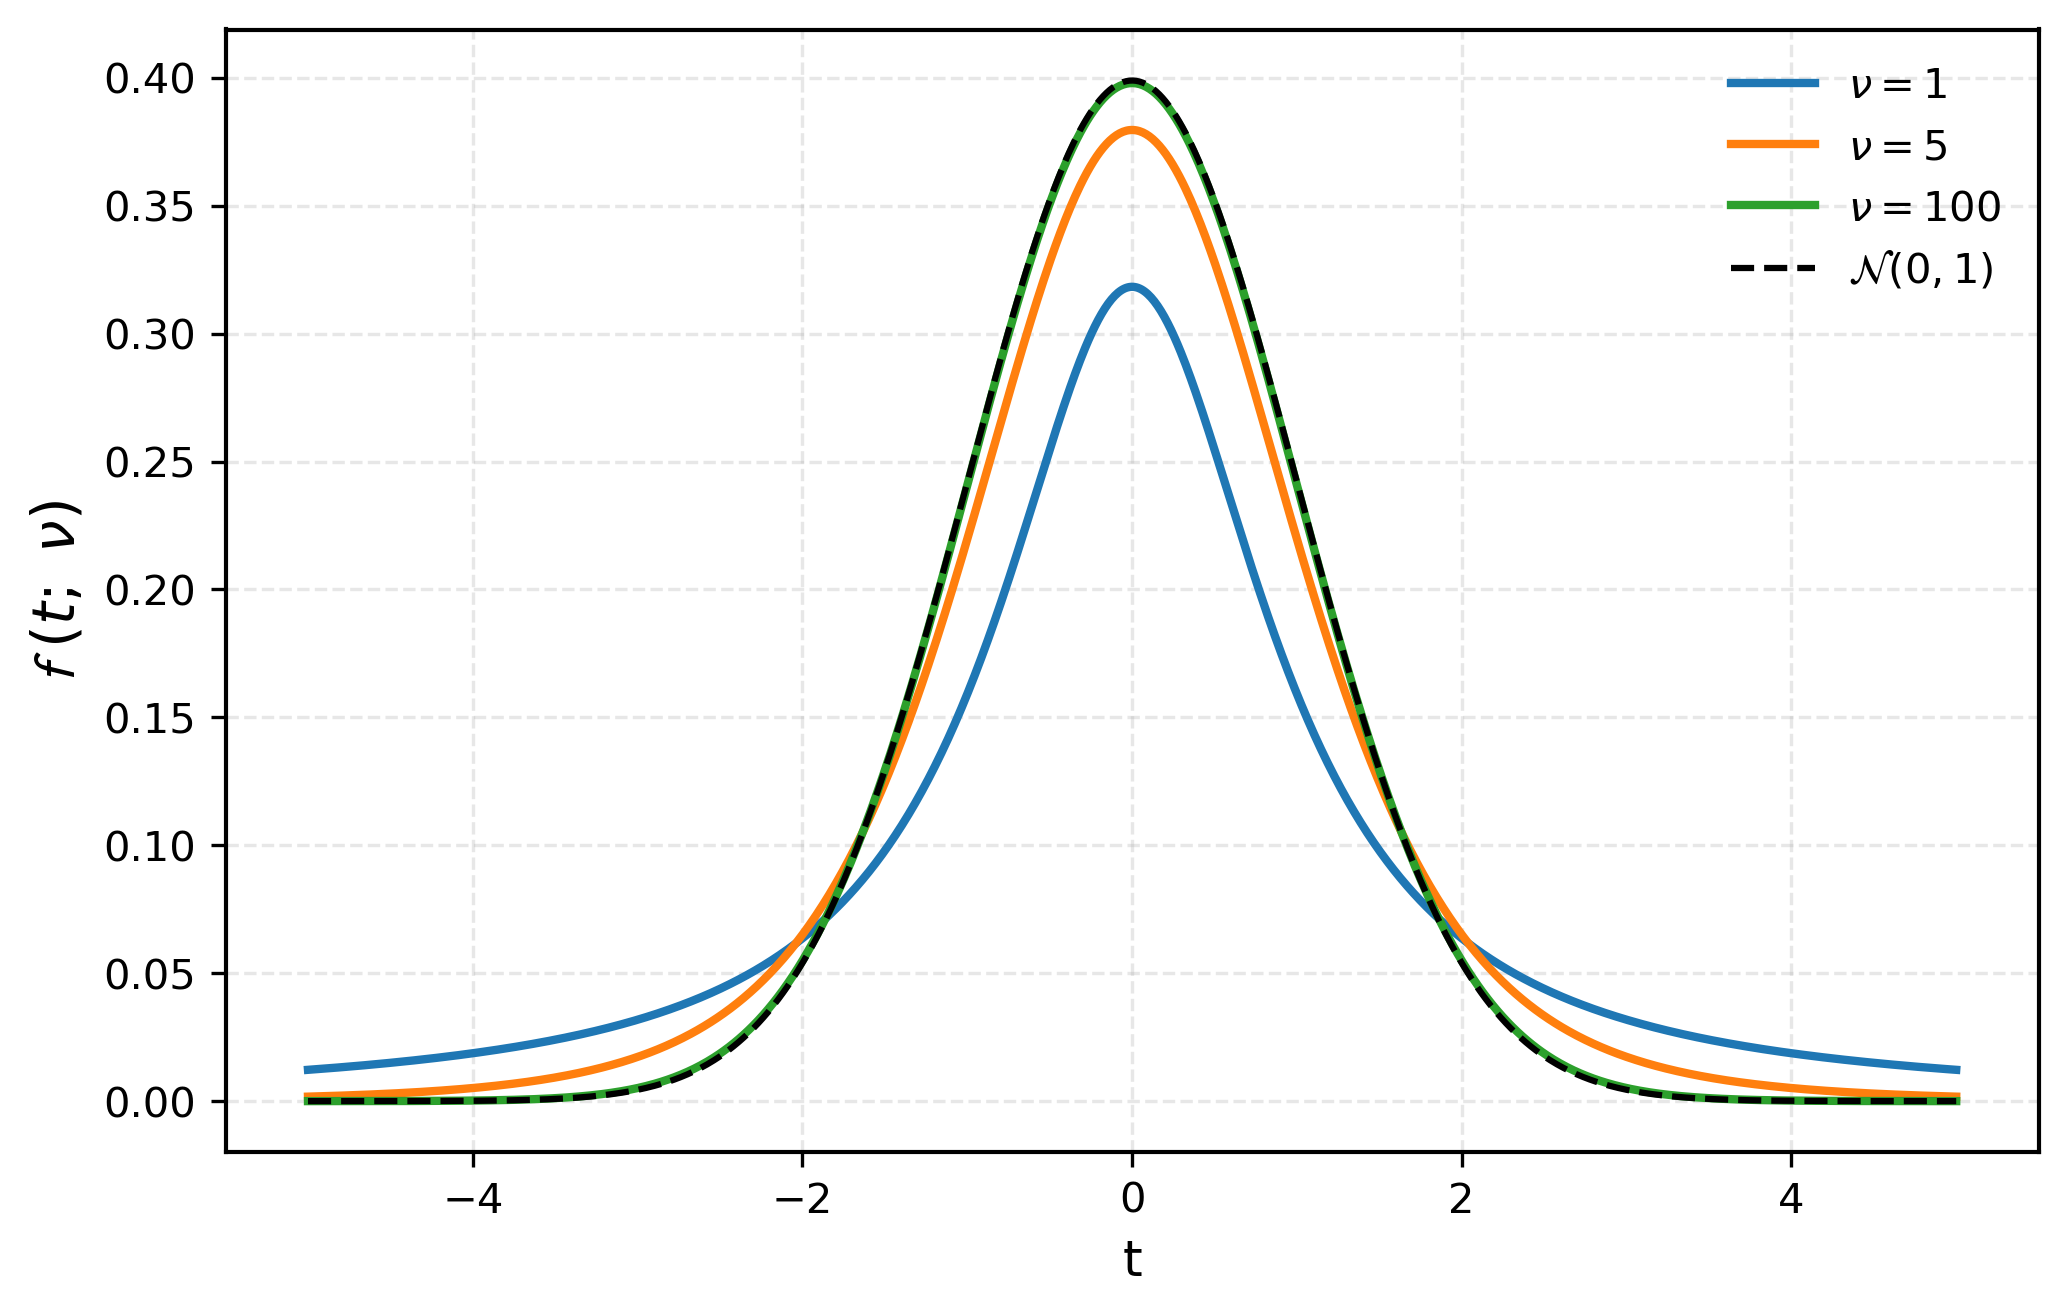
\includegraphics[width=0.7\textwidth]{figures/chapter4/t_distribution.png}
    \caption{Representation of the Student's t distribution, for different values of the degrees of freedom $\nu$.}
    \label{fig:t_distribution}
\end{figure}

\newpage

\subsection{Compare sample variances of two groups - Fisher's exact test}

Fisher’s exact test, introduced by Ronald A. Fisher in the 1930s, occupies a unique place in the statistical repertoire as a method built not on approximation, but on exact combinatorial reasoning. Designed to test for nonrandom association between two categorical variables in a 2x2 contingency table, the test calculates the exact probability of obtaining the observed configuration—or one more extreme—under the null hypothesis of independence. Unlike the chi-squared test, which relies on asymptotic assumptions, Fisher’s exact test makes no concession to large-sample theory, rendering it particularly well-suited for small datasets where expected counts may be sparse \cite{welch1947}.\\

The genesis of the test is as intellectual as it is practical. Fisher, with his characteristic synthesis of biological intuition and statistical rigor, crafted the test to address problems in genetics and experimental design. In particular, he sought a method that preserved the integrity of inference even when data were limited—a not uncommon situation in biological sciences of his time. His test exemplifies his broader philosophical stance: that statistical methods should be exact, and that inferences should reflect the full structure of the data, not rely on approximations that may distort conclusions.\\

In modern usage, Fisher’s exact test continues to shine in small-sample contexts—such as clinical trials, epidemiology, and case-control studies—where cell counts are low and the cost of misjudging association is high. Its continued relevance, despite the availability of powerful computational tools and large datasets, underscores a broader truth: that precision in reasoning often matters as much as the scale of inquiry. The test embodies an ideal of statistical craftsmanship, where fidelity to the data is preserved down to the last permutation.\\

\begin{figure}[ht]
    \centering
    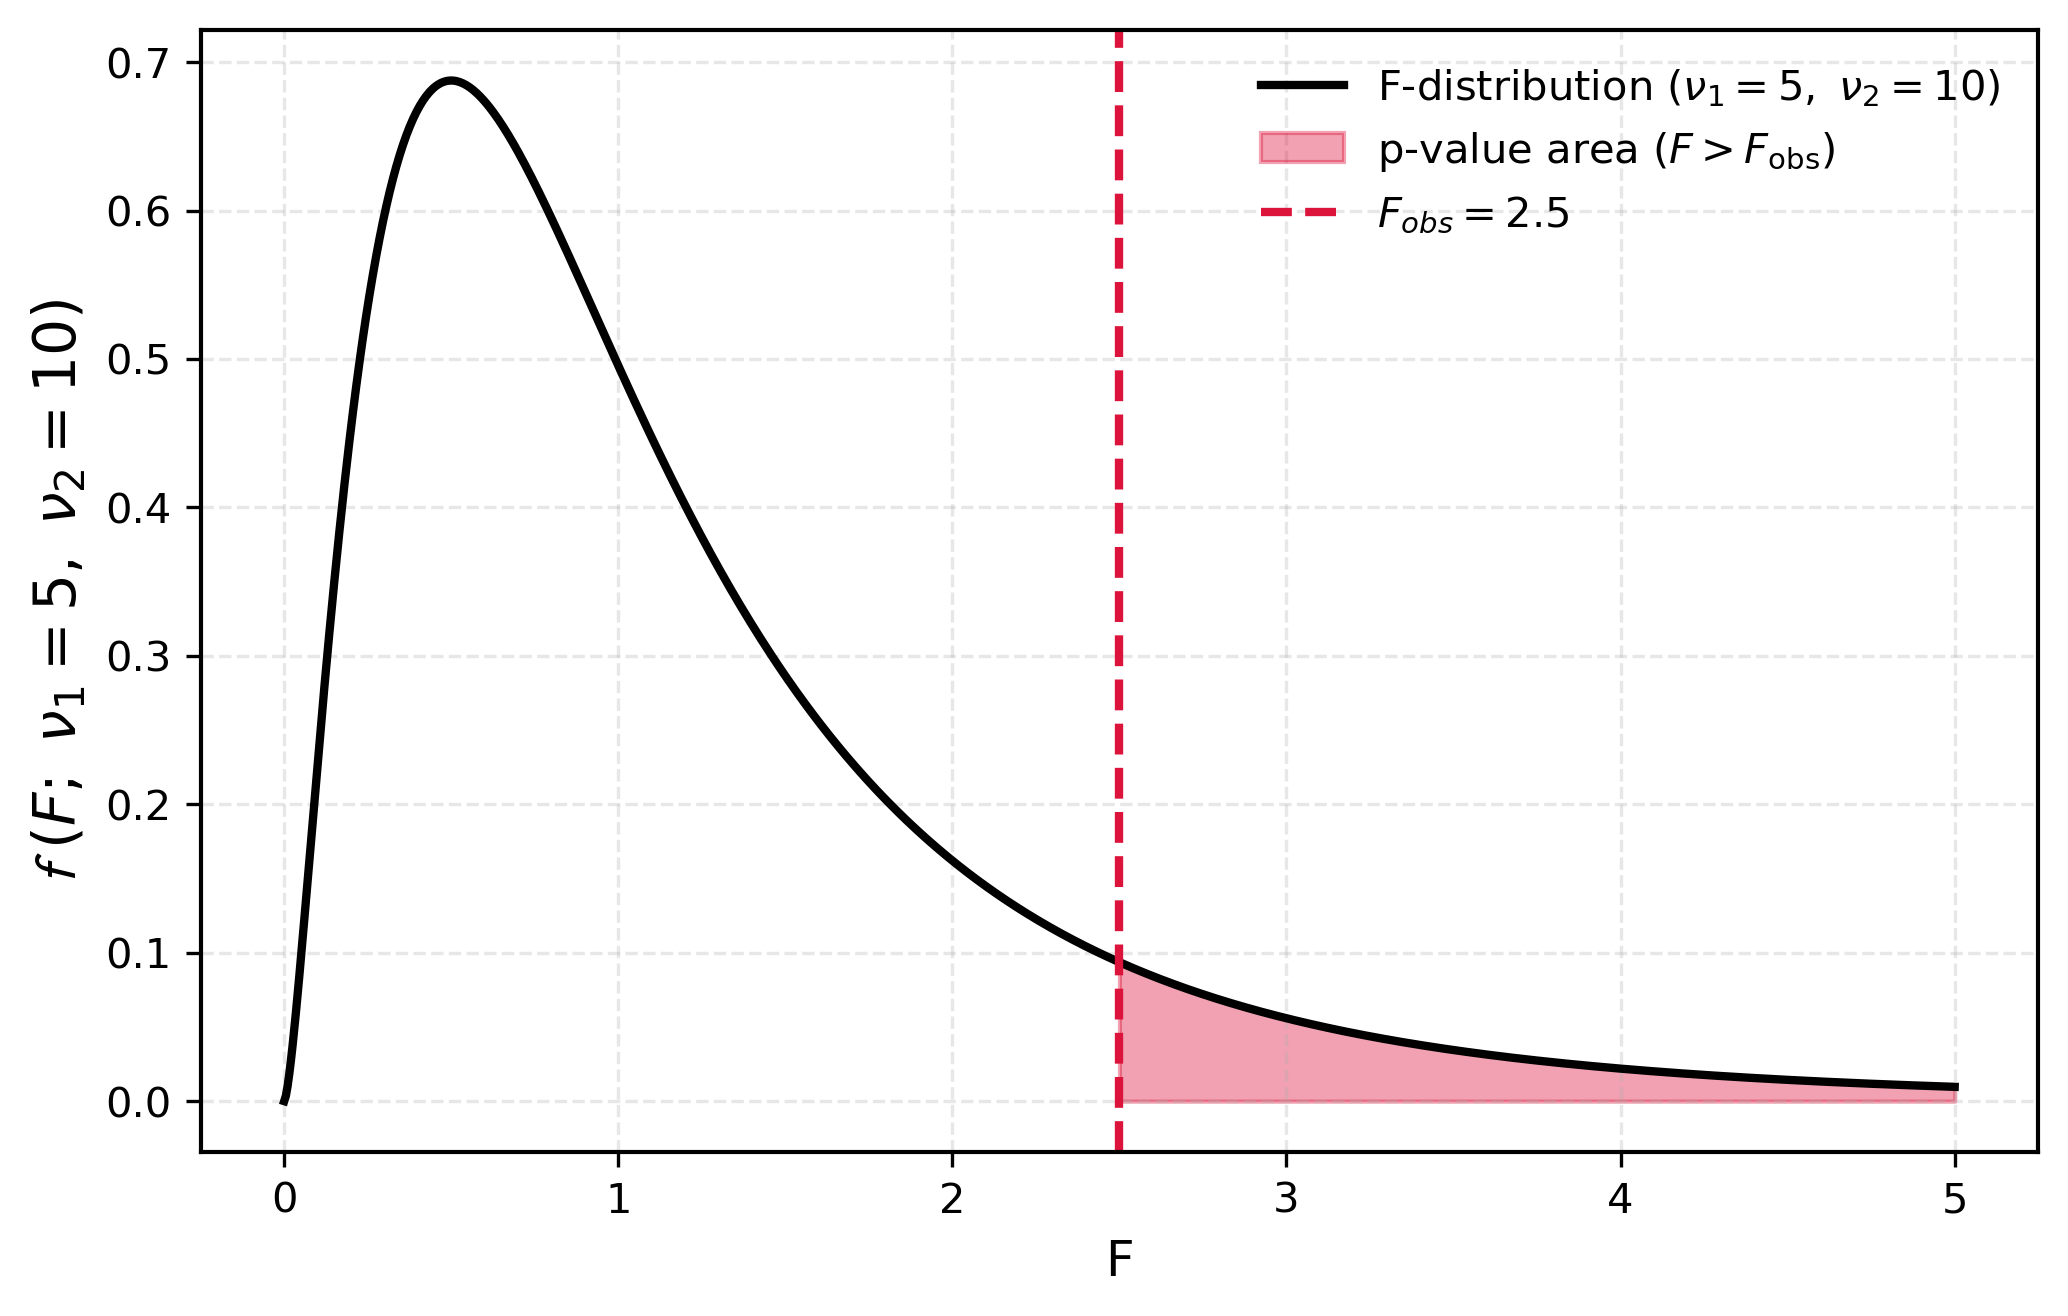
\includegraphics[width=0.7\textwidth]{figures/chapter4/f_test_one_tailed.png}
    \caption{Representation of the F statistic, following the Fisher distribution, for a particular value of the degrees of freedom ($\nu = 10$). The integral of the shadowed area represents the \textit{1-sided}, or \textit{1-tailed} p-value, as the probability of obtaining a result \textit{at least as extreme} as the one obtained $t_{obs}$.}
    \label{fig:f_test1}
\end{figure}

The next example we will encounter is an extension of the same question., The so-called \textit{Fisher t-test}, or just $F$ test, is used to determine whether the sample variances of two sets of observations are significantly different from one another. It assumes that the sample data are drawn from a normally distributed population.\\

The F statistic is a ratio of two independent variance estimates, each scaled by their respective degrees of freedom. It is used to test whether group variances (or group means, in ANOVA) differ significantly. The general form of the F statistic is:
\[
F = \frac{S_1^2 / \nu_1}{S_2^2 / \nu_2}
\]

where $s_1^{2}$ and $s_2^{2}$ are the sample variances, and the degrees of freedom are $d_1 = n_1 - 1$ and $d_2 = n_2 - 1$.\\

The computation of the p-value:
\[
p = \sum_{\text{extreme values}} \frac{\binom{a+b}{a} \binom{c+d}{c}}{\binom{n}{a+c}}
\]

Under the null hypothesis, the F statistic follows the F-distribution:

\[
F \sim F(\nu_1, \nu_2)
\]

and the p-value is computed as the upper-tail probability:

\[
p = P(F_{\nu_1, \nu_2} \geq F_{\text{obs}}) = \int_{F_{\text{obs}}}^{\infty} f_{F_{\nu_1, \nu_2}}(x)\,dx
\]

\subsection*{The F distribution}

When the assumption of equal variances is violated, the test statistic is:
\[
t = \frac{\bar{X} - \bar{Y}}{\sqrt{\frac{S_X^2}{n} + \frac{S_Y^2}{m}}}
\]
with an approximate degrees of freedom:
\[
\nu \approx \frac{\left(\frac{S_X^2}{n} + \frac{S_Y^2}{m}\right)^2}{\frac{(S_X^2/n)^2}{n - 1} + \frac{(S_Y^2/m)^2}{m - 1}}
\]

Under the null \( H_0: \mu_1 = \mu_2 \), the distribution of \( t \) is approximated by:
\[
t \sim t_{\nu}
\]
Distribution and computation of the p-value as defined above.

\newpage

\subsection{Compare variation on more than two groups - Fisher's ANOVA}

The analysis of variance, or ANOVA, is one of the 20th century's major statistical innovations, largely credited to Ronald Fisher, who formalized it in the 1920s while working at the Rothamsted Experimental Station. Its core purpose is to partition total variation in a dataset into components attributable to different sources—typically, between-group variation and within-group (error) variation. ANOVA provides a systematic method for comparing more than two means simultaneously, resolving what would otherwise require a series of pairwise t tests and an increasing risk of Type I error 
\cite{fisher1925}.\\

Conceptually, ANOVA represents a unifying idea: that observed data contain structure and randomness, and that the task of statistical inference is to disentangle them. It was particularly well-suited to agricultural experiments, where multiple treatments were applied across randomized plots, and variation needed to be measured with mathematical elegance and practical clarity. Fisher’s framework gave researchers a way to understand experimental results in terms of their statistical "signal," paving the way for rigorous design and interpretation across many scientific disciplines.\\

Today, ANOVA remains foundational in experimental science, psychology, and the social sciences. Its principles have expanded into more complex models—repeated measures, factorial designs, and mixed effects frameworks—but the essential logic endures. It is a statistical lens through which variability is not merely noise, but an object of structured inquiry. In this way, ANOVA reflects a deeper epistemological commitment: that difference can be measured, that structure can be inferred, and that complexity, when properly modeled, reveals its underlying form.\\

\begin{figure}[ht]
    \centering
    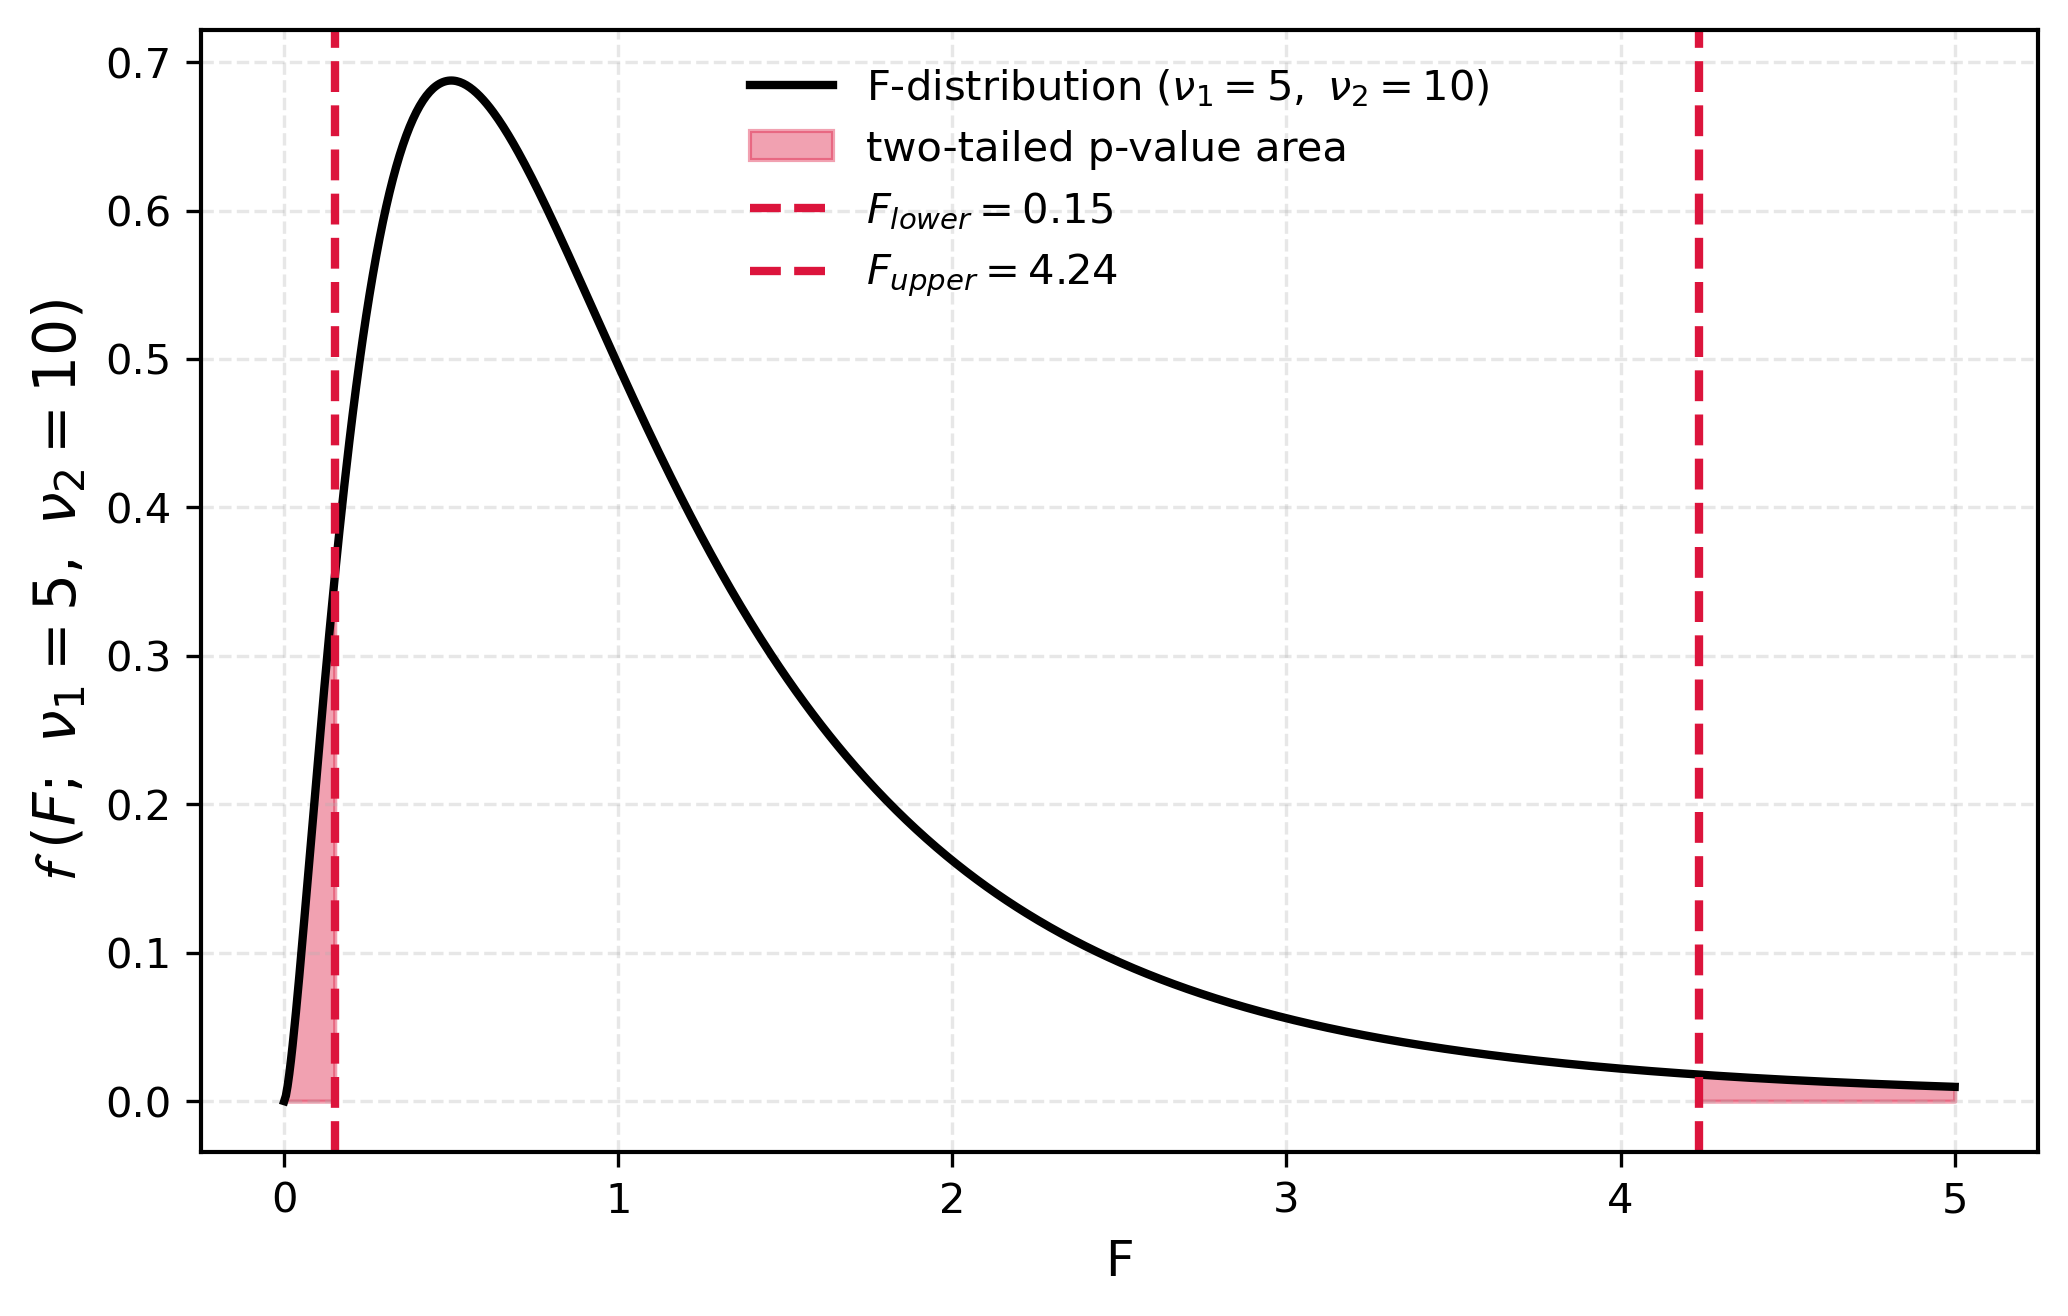
\includegraphics[width=0.7\textwidth]{figures/chapter4/f_test_two_tailed.png}
    \caption{Representation of the F statistic, following the Fisher distribution, for a particular value of the degrees of freedom ($\nu = 10$). The integral of the shadowed area represents the \textit{2-sided}, or \textit{2-tailed} p-value, as the probability of obtaining a result \textit{at least as extreme} as the one obtained $t_{obs}$.}
    \label{fig:f_test2}
\end{figure}

The so-called Analysis of Variance, one way ANOVA, or just ANOVA, is used to determine whether the variation of a dataset comes primary from variation within the samples themselves, or from variation between the groups. It is an extension of the Fisher test, where the F statistic is computed as:
\[
    f(x; d_{1}, d_{2}) = \frac{s_\text{between}^{2}}{s_\text{within}^{2}},
\]
where $s_1^{2}$ and $s_2^{2}$ are the sample variances, and the degrees of freedom are $d_1 = n_1 - 1$ and $d_2 = n_2 - 1$.\\

\[
F = \frac{MS_{\text{between}}}{MS_{\text{within}}} = \frac{SS_{\text{between}} / (k - 1)}{SS_{\text{within}} / (N - k)}
\]

where:
\begin{itemize}
  \item $SS_{\text{between}}$ is the sum of squares between groups,
  \item $SS_{\text{within}}$ is the sum of squares within groups,
  \item $k$ is the number of groups,
  \item $N$ is the total number of observations.
\end{itemize}

The computation of the p-value:
\[
p = \int_{F}^{\infty} f_{F_{df_1, df_2}}(x)\,dx = 1 - F_{F_{df_1, df_2}}(F)
\]

\subsection*{The F distribution}

Assume \( k \) groups with sample sizes \( n_i \) and group means \( \bar{X}_i \). The test statistic is:
\[
F = \frac{MS_{\text{between}}}{MS_{\text{within}}} = \frac{SS_{\text{between}} / (k - 1)}{SS_{\text{within}} / (N - k)}
\]
with:
\[
SS_{\text{between}} = \sum_{i=1}^{k} n_i (\bar{X}_i - \bar{X})^2, \quad SS_{\text{within}} = \sum_{i=1}^{k} \sum_{j=1}^{n_i} (X_{ij} - \bar{X}_i)^2
\]

Under \( H_0: \mu_1 = \mu_2 = \cdots = \mu_k \), the statistic follows:
\[
F \sim \mathcal{F}_{k-1, N-k}
\]
The PDF of the \( \mathcal{F}_{d_1, d_2} \) distribution is:
\[
f(x) = \frac{1}{\mathrm{B}(d_1/2, d_2/2)} \left(\frac{d_1}{d_2}\right)^{d_1/2} \frac{x^{d_1/2 - 1}}{\left(1 + \frac{d_1}{d_2}x\right)^{(d_1 + d_2)/2}}
\]
for \( x > 0 \).

Distribution and computation of the p-value as defined above.

\begin{figure}[ht]
    \centering
    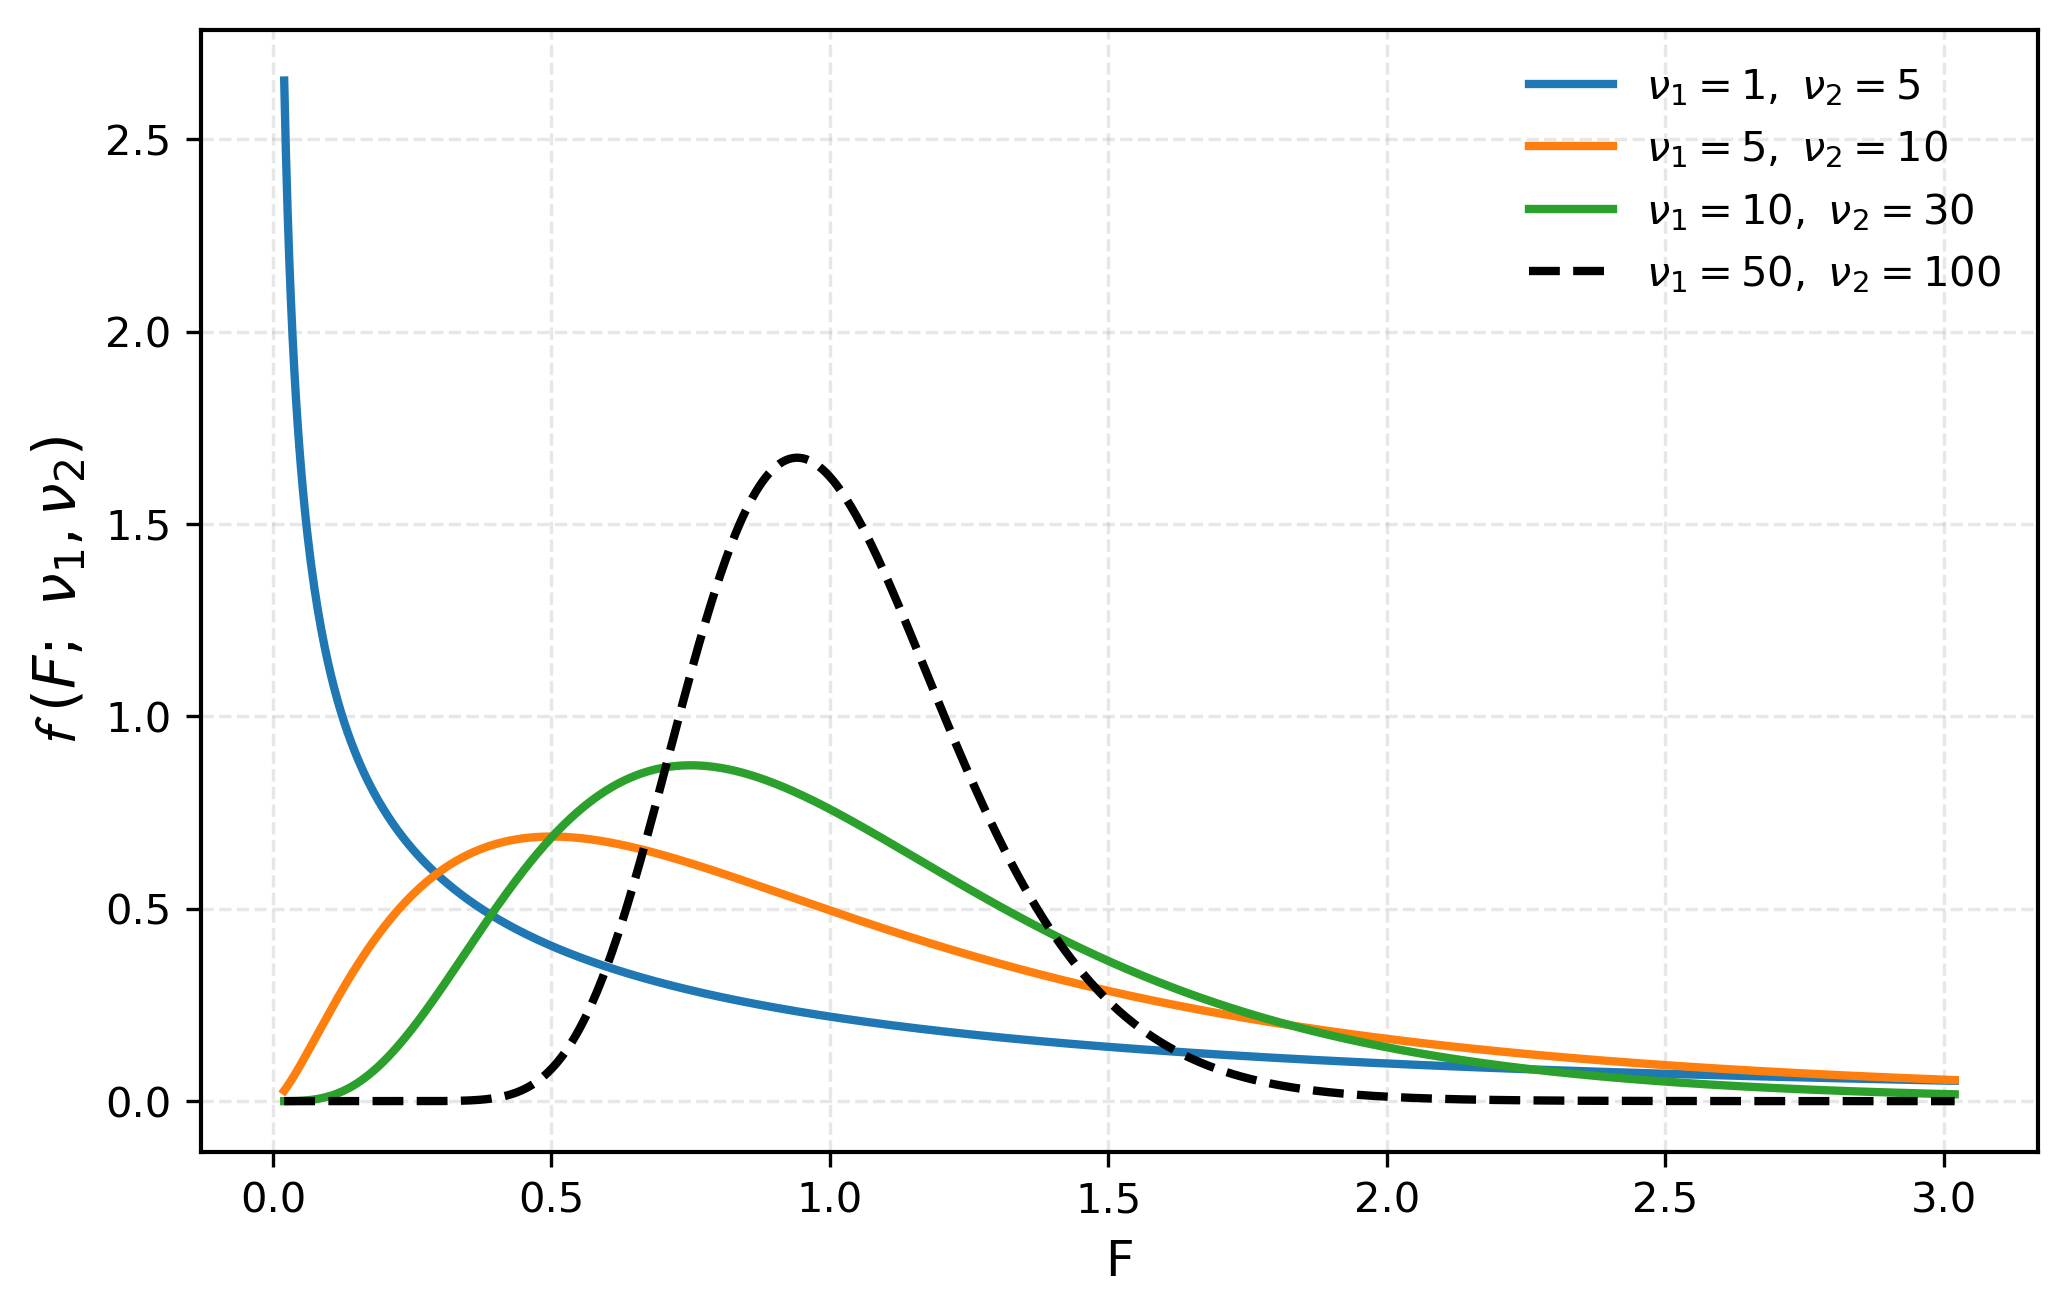
\includegraphics[width=0.7\textwidth]{figures/chapter4/f_distribution.png}
    \caption{Representation of the Fisher distribution, for different values of the degrees of freedom $\nu_1$, $\nu_2$.}
    \label{fig:f_distribution}
\end{figure}

\newpage

\subsection{Compare distributions and testing for normality - $\chi^{2}$ test}

The chi-squared test, with its roots in the work of Karl Pearson at the turn of the 20th century, stands as one of the earliest formal tests of goodness-of-fit and independence. Built on the comparison of observed frequencies to expected ones under a given hypothesis, the chi-squared statistic accumulates discrepancies between what is seen and what is statistically anticipated. It is asymptotic in nature, relying on the approximation of the chi-squared distribution, which becomes increasingly accurate with larger sample sizes and expected counts \cite{pearson1900}.\\

Pearson’s motivation was both mathematical and empirical: to provide a quantitative measure for evaluating how well a theoretical model matched observed data, particularly in biological contexts such as Mendelian genetics. His test became a cornerstone of categorical data analysis, offering a simple yet powerful method for detecting associations in contingency tables and deviations from expected distributions. Over time, the test was expanded and refined, notably by Fisher and Yates, but it has retained its essential character as a test of fit between expectation and observation.\\

In the present day, the chi-squared test continues to serve as an indispensable tool across fields as varied as market research, epidemiology, and political science. Its ability to handle complex tables and large datasets makes it well-suited to the modern data deluge. Yet its appeal also lies in its conceptual clarity: the squared discrepancy between what the world appears to be and what a hypothesis claims it should be. It is a statistical mirror, held up to the categorical world, revealing the tensions between model and reality with a cold but elegant precision.\\

\begin{figure}[ht]
    \centering
    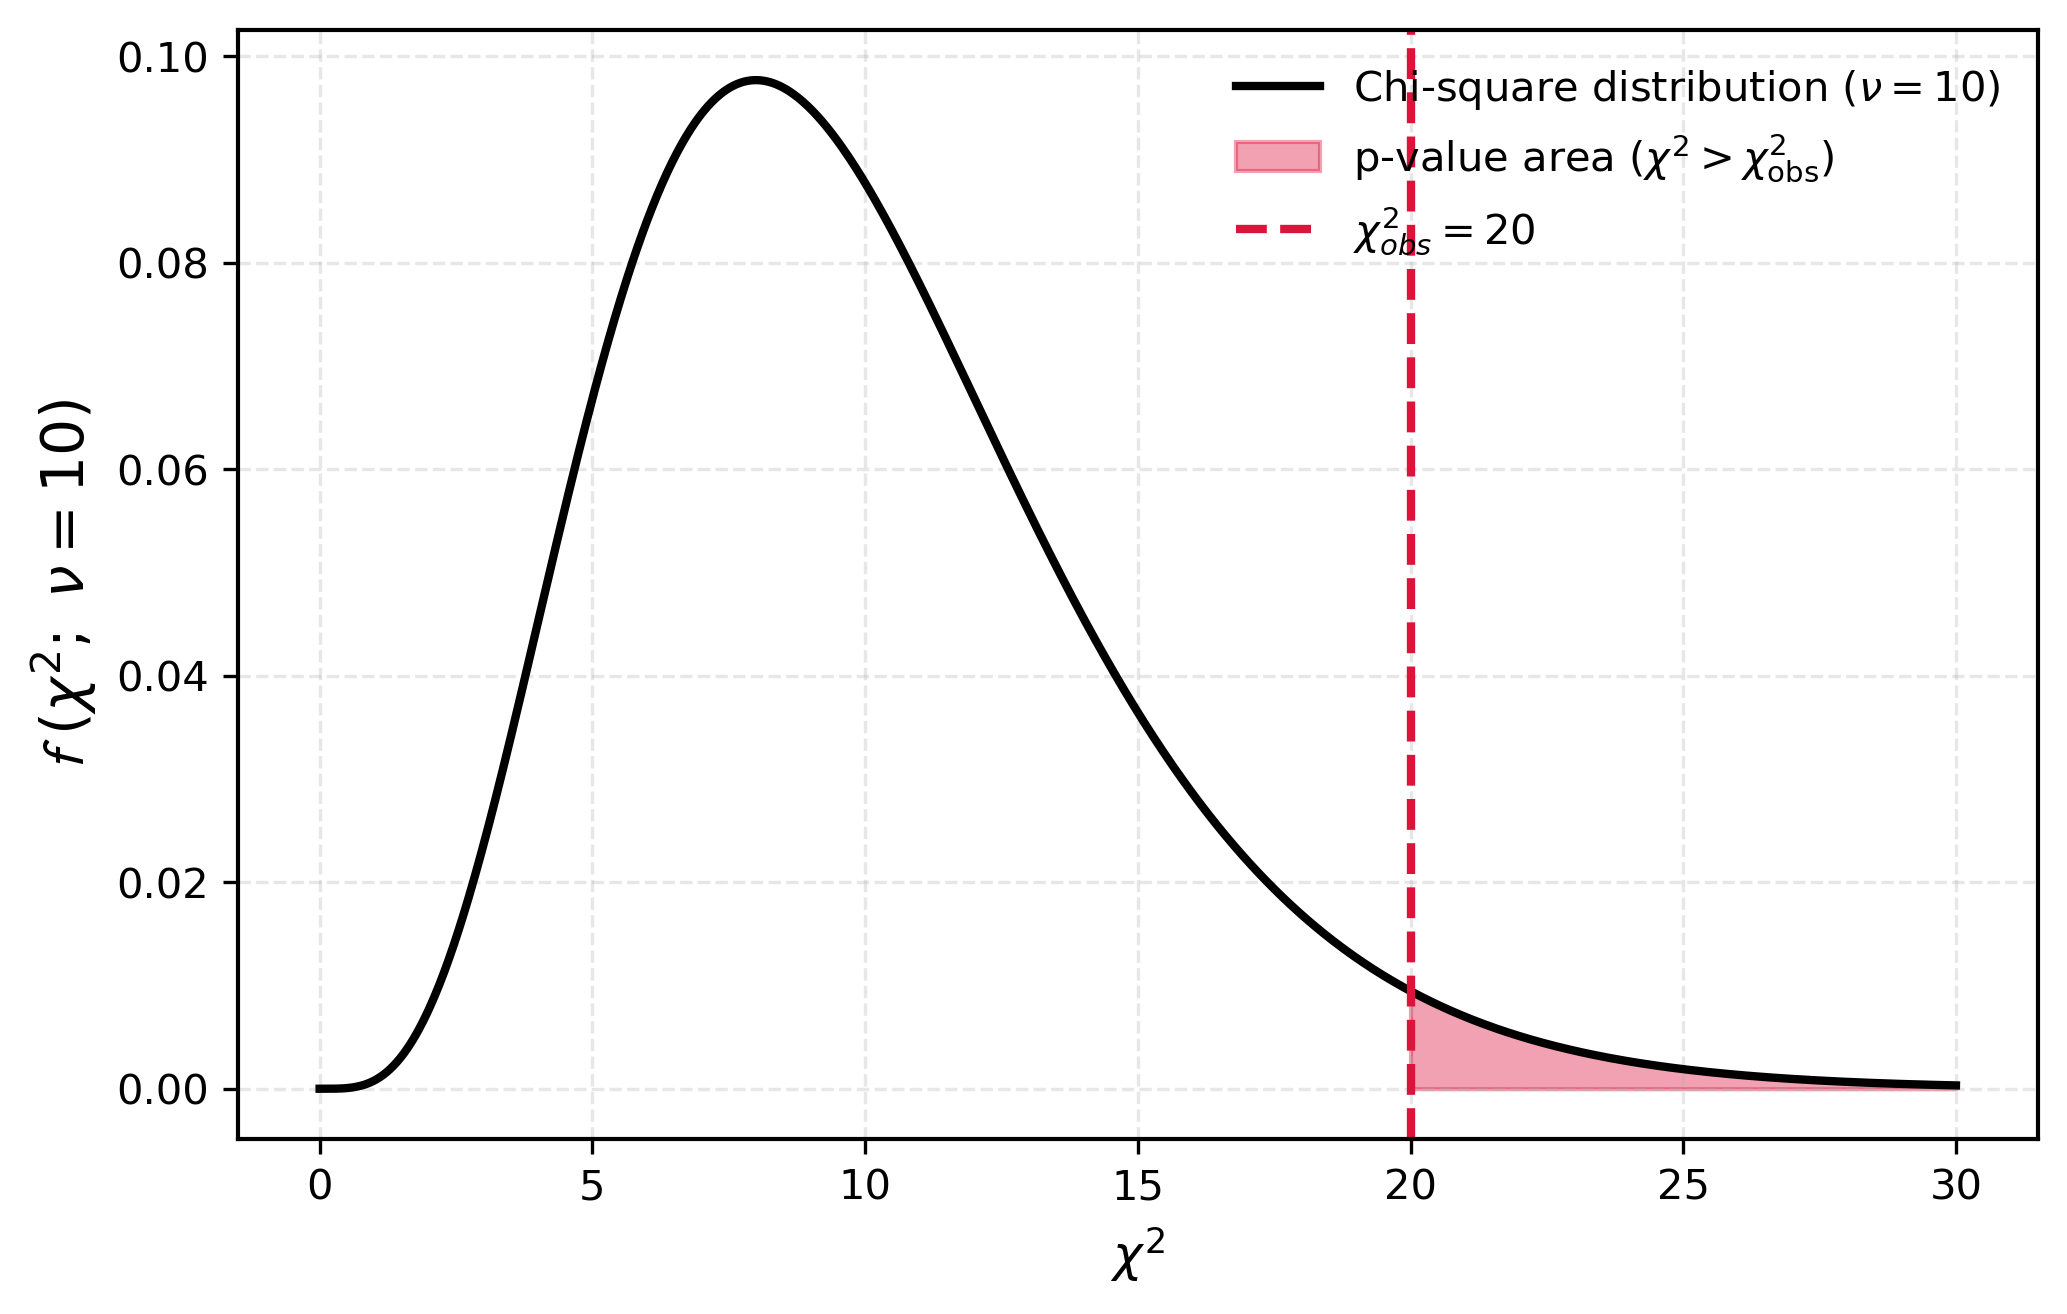
\includegraphics[width=0.7\textwidth]{figures/chapter4/chi2_test_one_tailed.png}
    \caption{Representation of the $chi^{2}$ statistic, following the Pearson $chi^{2}$ distribution, for a particular value of the degrees of freedom ($\nu = 10$). The integral of the shadowed area represents the \textit{1-sided}, or \textit{1-tailed} p-value, as the probability of obtaining a result \textit{at least as extreme} as the one obtained $chi^{2}_{obs}$.}
    \label{fig:chi2_test1}
\end{figure}

The so-called Pearson $\chi^{2}$-test is used to determine whether the set of observations is significantly different from some expected - or hypothesized - values. The $\chi^{2}$ statistic is given by:
\[
    \chi^{2}(x; N - 1) = \sum_{i = 1}^{N}\frac{(O_{i} - E{i})^{2}}{E_i},
\]
It is also used to test for normality and evaluate the goodness of a fit [...].\\\

\begin{figure}[ht]
    \centering
    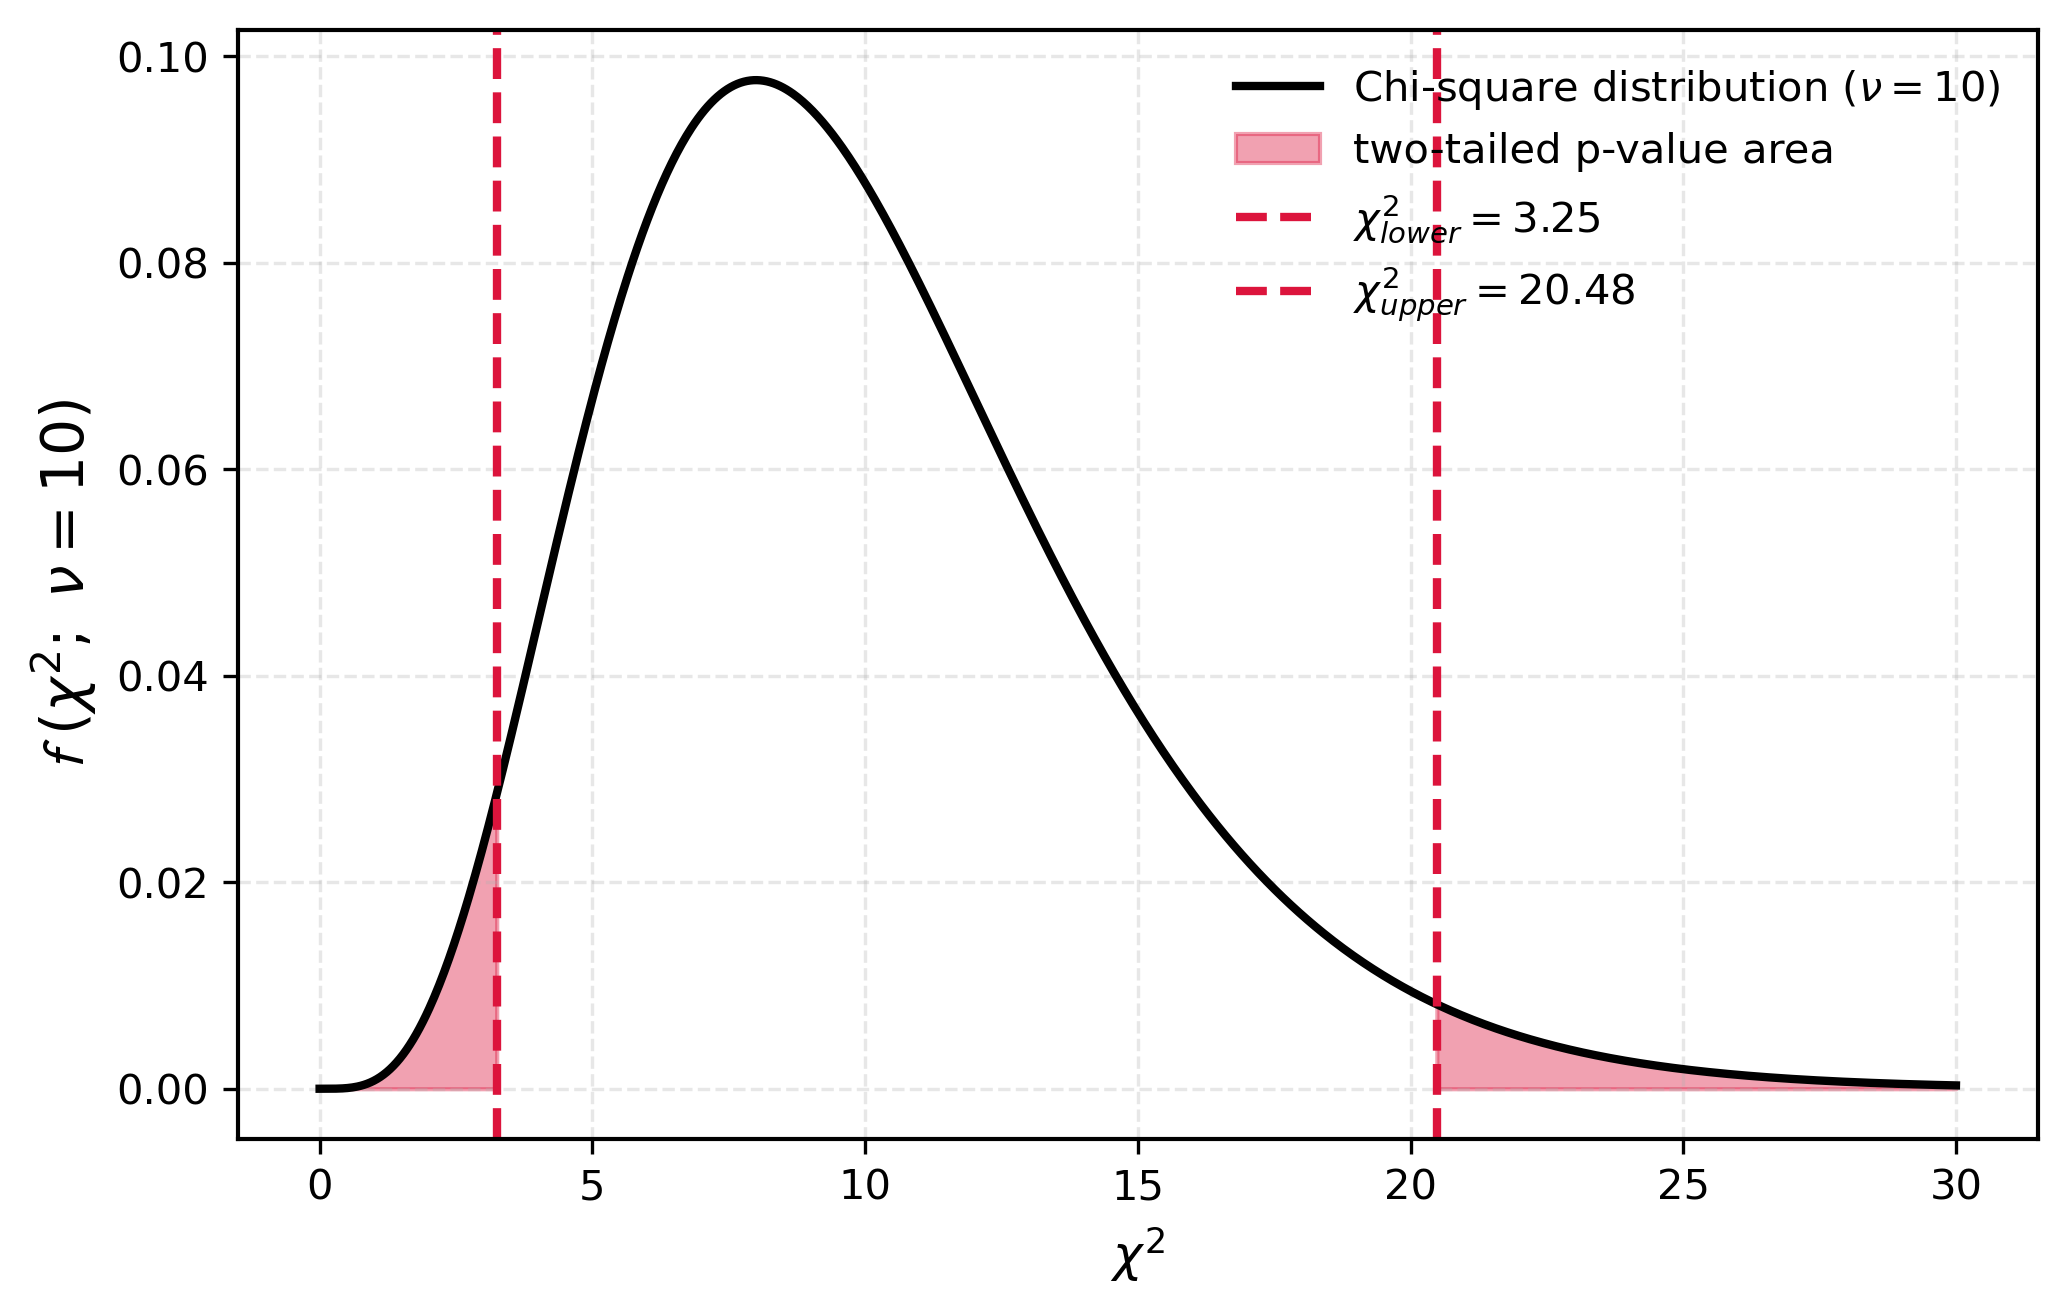
\includegraphics[width=0.7\textwidth]{figures/chapter4/chi2_test_two_tailed.png}
    \caption{Representation of the $chi^{2}$ statistic, following the Pearson $chi^{2}$ distribution, for a particular value of the degrees of freedom ($\nu = 10$). The integral of the shadowed area represents the \textit{2-sided}, or \textit{2-tailed} p-value, as the probability of obtaining a result \textit{at least as extreme} as the one obtained $chi^{2}_{obs}$.}
    \label{fig:chi2_test2}
\end{figure}

The computation of the p-value:
\[
p = \int_{\chi^2}^{\infty} f_{\chi^2_{df}}(x)\,dx = 1 - F_{\chi^2_{df}}(\chi^2)
\]

\subsection*{The $\chi^{2}$ distribution}

For observed \( O_{ij} \) and expected counts \( E_{ij} \) in an \( r \times c \) table, the test statistic is:
\[
\chi^2 = \sum_{i=1}^{r} \sum_{j=1}^{c} \frac{(O_{ij} - E_{ij})^2}{E_{ij}}
\]

Under the null hypothesis of independence, the distribution is:
\[
\chi^2 \sim \chi^2_{(r-1)(c-1)}
\]

The PDF of the chi-squared distribution with \( k \) degrees of freedom is:
\[
f(x) = \frac{1}{2^{k/2} \Gamma(k/2)} x^{k/2 - 1} e^{-x/2}, \quad x > 0
\]

Distribution and computation of the p-value as defined above.

\begin{figure}[ht]
    \centering
    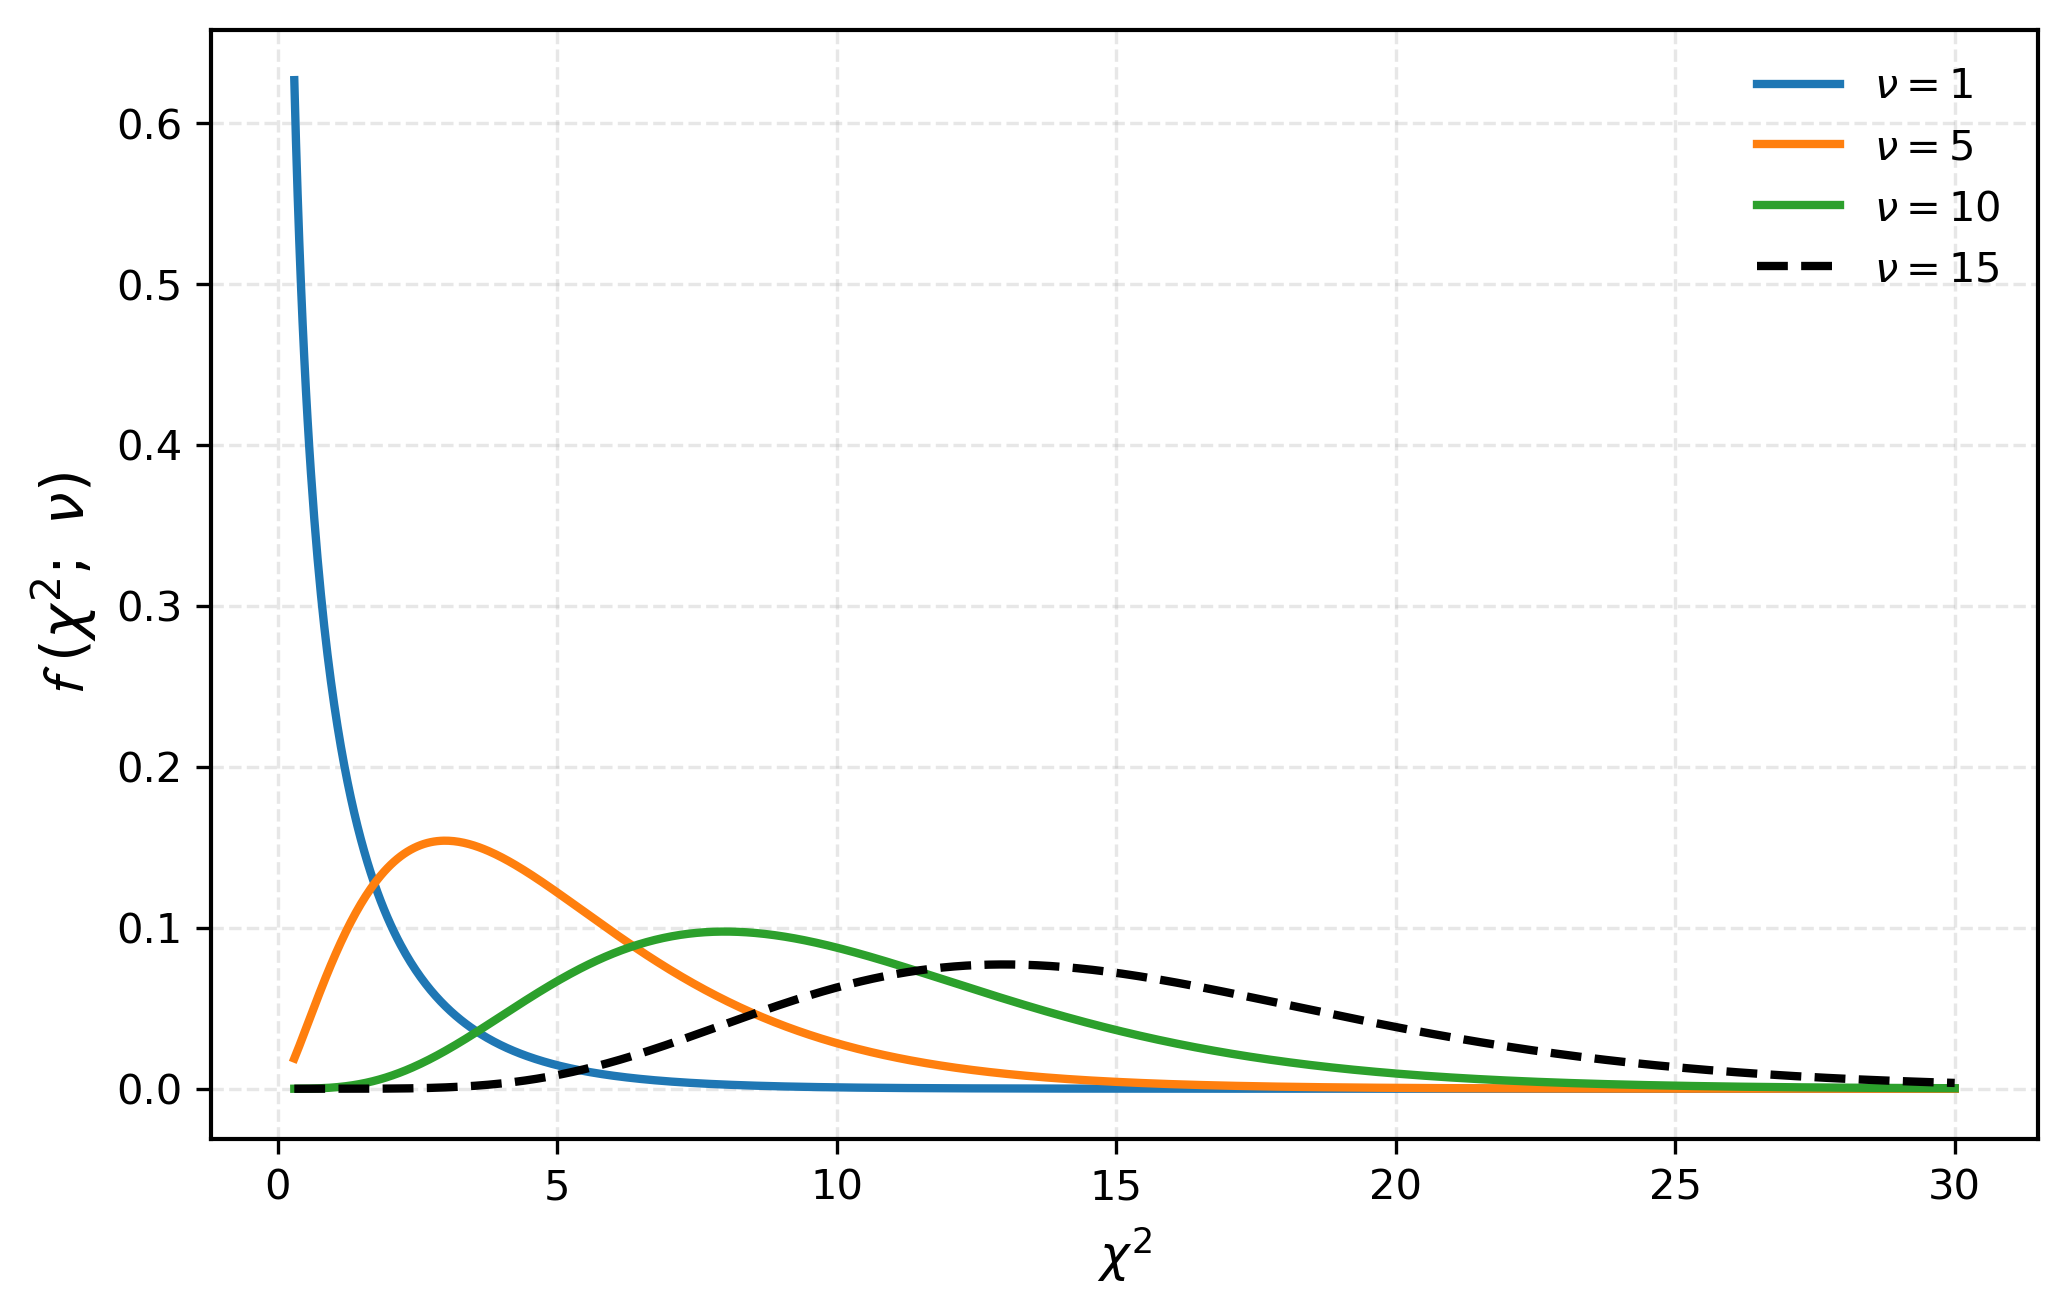
\includegraphics[width=0.7\textwidth]{figures/chapter4/chi2_distribution.png}
    \caption{Representation of the $chi^{2}$ distribution, for a particular value of the degrees of freedom ($\nu = 10$).}
    \label{fig:chi2_distribution}
\end{figure}

\newpage

\section{Parametric and non-parametric}

Parametric and non-parametric

\begin{enumerate}

\item \textbf{Student’s *t*-Test (One-Sample and Two-Sample)}\\
Introduced by William S. Gosset under the pseudonym “Student” in his seminal paper \cite{student1908}, this test allows inference on population means when the standard deviation is unknown and the sample size is small. The two-sample version compares the means of two independent groups under assumptions of normality and equal variances.\\
\textit{Non-parametric alternative:} The \textbf{Mann–Whitney U test} (also called the Wilcoxon rank-sum test) for independent samples, and the \textbf{Wilcoxon signed-rank test} for paired or single-sample symmetry testing.

\item \textbf{Fisher’s Exact Test}\\
Formulated by R. A. Fisher in his 1935 treatise on experimental design \cite{fisher1935}, this exact test computes the hypergeometric probability of a given 2x2 contingency table under the null hypothesis of independence. It is particularly suited for small samples, where asymptotic methods like chi-squared tests may not be valid.\\
\textit{Non-parametric alternative:} The test is already exact and non-parametric; however, \textbf{Barnard’s exact test} is sometimes proposed as a more powerful alternative in small-sample settings.

\item \textbf{Analysis of Variance (ANOVA)}\\
Fisher also introduced ANOVA in his earlier work \cite{fisher1925}, laying the foundation for modern experimental statistics. ANOVA decomposes total variation into between-group and within-group components, enabling testing of the equality of multiple means.\\
\textit{Non-parametric alternative:} The \textbf{Kruskal–Wallis H test}, which operates on ranks rather than means, is used when ANOVA assumptions (e.g., normality or homoscedasticity) are violated.

\item \textbf{Chi-Squared Test}\\
Originally proposed by Karl Pearson in 1900 \cite{pearson1900}, the chi-squared test evaluates how observed frequencies compare to expected frequencies under a null model of independence or goodness-of-fit. It is widely used in contingency table analysis and categorical data testing.\\
\textit{Non-parametric alternative:} While the chi-squared test is non-parametric in principle, \textbf{Fisher’s exact test} is often preferred for 2x2 tables with small expected counts.

\item \textbf{Welch’s *t*-Test (Unequal Variance Version)}\\
To address the limitations of assuming equal variances in the classical *t*-test, Welch proposed a generalization in 1947 \cite{welch1947} that remains robust under heteroscedasticity. It uses a weighted estimate of variance and adjusts the degrees of freedom accordingly.\\
\textit{Non-parametric alternative:} The \textbf{Mann–Whitney U test} again serves as a distribution-free method for comparing central tendencies when variance assumptions fail.

\end{enumerate}

\newpage

\section{Comparing data and normalization}

Comparing data and normalization

\newpage

\subsection*{Exercises}

\textbf{1.} Exercise [...].\\

\textbf{2.} Exercise [...].\\

\textbf{3.} Exercise [...].\\

\newpage

\subsection*{Solutions}

\textbf{1.} Solution [...].\\

\textbf{2.} Solution [...].\\

\textbf{3.} Solution [...].\\



% Chapter - Introduction to bayesian probability .........................................................................................................................................................
\chapter{Introduction to bayesian probability}

\epigraph{\textit{Probability statements are just summaries of repeated observations.}}{— W. V. Quine}

\section{Bayesian vs frequentist}

So far we have discussed probability and statistics assuming the \textit{frequentist} definition of probability. That is, we have implicitly assumed that the probability, that number we make up to represent uncertainty, can be defined just as a ratio of the number of times we get a specific result, and the total number of observations. In the classic example of the coins, that we used in Chapter 2 to define probability in the first place, we are assuming, for instance, that the coin is fair. In the frequentist interpretation, probability is defined as the long-run relative frequency of an event occurring. For example, in the case of a fair coin:

\[
P(\text{H}) = \lim_{n \to \infty} \frac{\text{Number of H in } n \text{ tosses}}{n} = 0.5
\]

This approach assumes repeated experiments and well-defined probabilities that do not change. But if we start tossing the same coin again and again, and encounter that the ration of heads and tails is significantly different than 0.5, maybe we should start question that first assumption in the first place. Frequentist statistics might say we don't have enough data yet. But can we make a meaningful guess using prior knowledge and observed data? \\

This way of understanding probability, as founded in some \textit{prior beliefs} that can be updated as new evidence comes available, is normally referred to as \textit{bayesian} approach, or bayesian definition. It was developed by Thomas Bayes, a British mathematician who worked primarily on [...]. Early mathematicians like Pascal and Fermat formalized the idea of quantifying uncertainty. Over time, two main schools emerged: the frequentists, who interpret probability as the long-run frequency of events, and the Bayesians, who interpret probability as a degree of belief or certainty about an event. Thomas Bayes introduced the idea of updating probabilities based on new evidence. His work was published posthumously and it was later popularized by Laplace, and it is nowadays referred as the \textit{Bayes’ theorem}. Both approaches offer useful perspectives for understanding and analyzing uncertainty.\\

The frequentist approach relies on repeating experiments many times and observing how often events occur to estimate probabilities. It treats probability as an objective property of the physical world. In contrast, Bayesian probability treats it as a subjective measure of belief, updated as new data arrives. This difference influences how we interpret data and make predictions, and understanding both is important for a well-rounded grasp of statistics.\\

Frequentist methods often focus on long-run behaviour, like estimating probabilities from observed data or constructing confidence intervals. Bayesian methods combine prior knowledge (beliefs before seeing data) with observed data to update our understanding. In practice, both methods are used and combined and depending on the problem context.\\

\newpage

\section{The Bayes' Rule}

The second one — working backwards from results to reasons, purely, inferential — is what Bayes’ Theorem is all about. It’s how we reconstruct from data the underlaying phenomenology. From now on, w we will ask not only what is the probability for some event to take place, but what is the probability of that event happening \textit{given that} some other phenomena, some hypothesized scenario, is already taking place.\\

Bayes’ theorem appears often in biological sciences and medical tests, search engines, and in most data analysis problems when experimental results requiere interpretation and inference. It’s the engine behind how we learn from evidence, and once we understand it, we will start seeing it everywhere — from everyday decisions to machine learning. Its mathematical form can be written as follows. The \textit{conditional}, or \textit{posterior} probability of observing some some event $E$ happening, given some \textit{prior} knowledge, or hypothesis $H$ was true, is given by:

\begin{equation}
P(E|H) = \frac{P(H|E) \cdot P(H)}{P(E)}
\end{equation}

Where:
\begin{itemize}
  \item $P(E|H)$ is the probability of event $E$ given that $H$ has occurred (the \textbf{posterior}).
  \item $P(H|E)$ is the probability of event $E$ given $H$ (the \textbf{likelihood}).
  \item $P(H)$ is the probability of $H$ before seeing $E$ (the \textbf{prior}).
  \item $P(E)$ is the total — also called \textit{marginal} — probability of $E$ occurring (the \textbf{evidence}).
\end{itemize}

With bayesian probability we face now a complete different perspective. Bayesian probability treats probability as a degree of belief or confidence in a hypothesis. Rather than only relying on infinite repeated experiments, it allows us to update our beliefs in light of new evidence. Unlike the frequentist approach, we can incorporate prior information and handle small datasets. Bayes’ Rule provides the mechanism for updating beliefs.\\

Let's illustrate this with an example. Imagine we are given two dice, let's call them $D_1$ and $D_2$. The first one, $D_1$, is a far dice, and hence the probability of rolling any of the faces is uniformly distributed, all with probability $\frac{1}{6}$. But $D_2$ is biased, such that the probability of rolling a 6 is almost half the times. We can write the likelihoods of rolling a 6 in both cases, in the following way:
\begin{itemize}
  \item Dice 1 is \textbf{fair}, so $P(6|D_1) = \frac{1}{6}$.
  \item Dice 2 is \textbf{biased}, so $P(6|D_2) = \frac{1}{2}$.
\end{itemize}

We randomly pick one die, with no reason to favor either. Since we have just two options, the probability of choosing blindly one or the other — we will call this the \textit{prior} probability — is
\[
P(D_1) = P(D_2) = \frac{1}{2}
\]

Then, after that choice is made, we roll the dice and get a 6. And here is the question: What are the chances that we picked the biased die? Let's carefully define the prior beliefs and likelihoods, so that we can apply the Bayes rule. Let:

\begin{itemize}
  \item $H_1$: You picked the fair die.
  \item $H_2$: You picked the biased die.
  \item $E$: You rolled a 6.
\end{itemize}

We want to find $P(H_2 | E)$ — the probability that the die is biased given that we rolled a 6.\\

Using Bayes’ Theorem:

\[
P(H_2 | E) = \frac{P(E | H_2) \cdot P(H_2)}{P(S)}
\]

First, we calculate the marginal probability $P(E)$ — the overall chance of rolling a 6:

\[
P(E) = P(E | D_1) \cdot P(H_1) + P(E | D_2) \cdot P(H_2) = \frac{1}{6} \cdot \frac{1}{2} + \frac{1}{2} \cdot \frac{1}{2}
= \frac{1}{12} + \frac{1}{4} = \frac{1}{3}
\]

Now apply Bayes' Theorem:

\[
P(H_2 | E) = \frac{\frac{1}{2} \cdot \frac{1}{2}}{\frac{1}{3}} = \frac{1}{4} \div \frac{1}{3} = \frac{3}{4}
\]\\

Even though both dice had the same chance of being picked, rolling a 6 strongly points to the biased die. Bayes’ Theorem helped us turn a gut feeling into a solid number: a \textbf{75\% chance} that the die was biased. Bayes’ Theorem isn’t just math — it’s a mindset. It’s how we learn, adapt, and update our understanding when the world surprises us. Once you see it in action, it becomes a natural way to think about uncertainty and evidence.

\begin{itemize}
    \item \textbf{Frequentist}: Probability as long-run frequency.
    \item \textbf{Bayesian}: Probability as belief, updated with evidence.
\end{itemize}

\newpage

\section{Bayesian vs frequentist}
Bayesian vs frequentist.

\newpage

\section{Computing posteriors}
Computing posteriors.

\subsection*{Exercises}

\textbf{1.} Exercise [...].\\

\textbf{2.} Exercise [...].\\

\textbf{3.} Exercise [...].\\

\newpage

\subsection*{Solutions}

\textbf{1.} Solution [...].\\

\textbf{2.} Solution [...].\\

\textbf{3.} Solution [...].\\

\section{Stochasticity and Markov processes}

The world around us is full of uncertainty. Facing questions like, will it rain tomorrow? Will a cell divide or die? Will a water drop fall in the same place after some time, or somewhere near? In many cases, the best we can do is talk in terms of probabilities — not certainties. This is where the idea of \textit{stochasticity} comes again, and why mathematicians of the 20th century deeply revisited its meaning. Stochasticity normally means randomness. From now on, we will define a stochastic process as a system that evolves over time in a way that involves some degree of randomness. Instead of asking, “What exactly will happen?” we ask, “What is likely to happen?”\\

Stochasticity means randomness or unpredictability in a system, as we have seen in previous chapters. But from now on, and following the work of mathematicians like Markov in the early 20th century, we will address it with a bit more subtlety. Now we will think about \textit{stochasticity} as randomness or unpredictability in a system, in opposition to deterministic systems, where future states are exactly determined by current conditions, stochastic systems incorporate randomness, making their outcomes probabilistic. Understanding stochasticity helps in modeling real-world phenomena where uncertainty is inherent, such as stock prices, weather, or population dynamics.\\

Even though the study of chance and probability can be trace to very ancient roots, as we have seen in previous chapter, \textit{stochasticity} as randomness or unpredictability in a system, in opposition to deterministic systems, began in the early 20th century, as mathematicians sought to model systems evolving randomly over time. Early work by Andrey Markov introduced Markov chains—models where the future depends only on the present state, not the past history. These models became fundamental in fields such as physics, biology, economics, and computer science for understanding complex systems affected by randomness. Over time, stochastic processes have grown into a broad discipline, providing tools for predicting and analyzing uncertain, evolving phenomena.\\

Markov processes are a class of stochastic models with the “memoryless” property—the future state depends only on the current state. This simplification makes analysis feasible and is surprisingly accurate for many systems. Markov chains are used in algorithms, queueing theory, genetics, and many other fields to describe how systems evolve step-by-step in time.\\

Many systems in nature and society follow patterns, but with noise, surprises, or variability. Markov models give us a way to describe and work with such systems — mathematically and intuitively. Imagine you're trying to predict the weather. If it’s sunny today, what are the chances it’ll be sunny tomorrow? What if it was rainy? Markov models help us answer these kinds of questions using a simple but powerful idea:\\

\textbf{The future depends only on the present — not the past.}\\

This is called the \textbf{Markov property}. A Markov model is a way to describe systems that move between states (like "sunny", "rainy", or "cloudy") with certain probabilities. Markov models are useful when things change over time in a somewhat random, yet patterned, way. Think of weather patterns, stock market movements, DNA sequences, pages people click on in a website, as examples. Even if we can’t predict everything perfectly, we can model how likely one thing is to follow another.\\

The key ingredients of a Markov model are:
\begin{itemize}
  \item A list of possible \textbf{states} (e.g., sunny, rainy), we will write as vectors.
  \item A \textbf{transition matrix}, encoding the probabilities of moving from one state to another.
\end{itemize}

Let's illustrate with a simple example. Let's try to predict weather in the following day, assuming stochasticity and knowledge of the previous states. For simplicity let’s say the weather can be either sunny ($S$) or rainy ($R$). And based on past data, we know:

\[
\text{Transition Matrix} =
\begin{bmatrix}
P(\text{Sunny} \rightarrow \text{Sunny}) & P(\text{Sunny} \rightarrow \text{Rainy}) \\
P(\text{Rainy} \rightarrow \text{Sunny}) & P(\text{Rainy} \rightarrow \text{Rainy})
\end{bmatrix}
=
\begin{bmatrix}
0.8 & 0.2 \\
0.4 & 0.6
\end{bmatrix}
\]

This means:
\begin{itemize}
  \item If today is Sunny, there's an 80\% chance tomorrow will also be Sunny, and 20\% chance of Rain.
  \item If today is Rainy, there's a 40\% chance it clears up, and a 60\% chance it stays rainy.
\end{itemize}

Suppose today is Sunny. We can represent our current state as a vector:

\[
\text{Today} = \begin{bmatrix} 1 & 0 \end{bmatrix}
\]

Then tomorrow’s prediction is:

\[
\text{Tomorrow} = \text{Today} \times \text{Transition Matrix} = 
\begin{bmatrix} 1 & 0 \end{bmatrix} \times
\begin{bmatrix}
0.8 & 0.2 \\
0.4 & 0.6
\end{bmatrix}
=
\begin{bmatrix}
0.8 & 0.2
\end{bmatrix}
\]

So there's an 80\% chance of Sun, 20\% chance of Rain tomorrow.\\

Markov models help us make predictions, model uncertainty, and understand patterns in time-based data. They are a stepping stone to more complex tools like Hidden Markov Models (HMMs), used in speech recognition, bioinformatics, and more [...].\\

Markov models are simple but powerful tools. They help us model systems that evolve over time, assuming that the next state only depends on the current one. Whether you’re analyzing text, tracking a robot, or predicting rain, the Markov assumption can be surprisingly useful [...].

\section{Markov chains}
Markov chains.

\section{Hidden Markov models}
Hidden Markov models.

\newpage

\subsection*{Exercises}

\textbf{1.} Exercise [...].\\

\textbf{2.} Exercise [...].\\

\textbf{3.} Exercise [...].\\

\newpage

\subsection*{Solutions}

\textbf{1.} Solution [...].\\

\textbf{2.} Solution [...].\\

\textbf{3.} Solution [...].\\



% Appendix .........................................................................................................................................................
\appendix



% Chapter: Vectors and matrices
\chapter{Appendix: Vectors and matrices: a quick review}

\section{The roots and rise of algebra}

Algebra and vectors form two essential branches of mathematics, each with a rich history and deep connections to the physical and abstract worlds. Algebra is the language of generality and structure, the art of manipulating symbols to uncover patterns and relationships. Vectors, on the other hand, provide the geometry of direction and magnitude---a way of describing the multi-dimensional spaces in which physical and conceptual systems evolve. Together, they offer a powerful framework for solving problems in mathematics, physics, engineering, and beyond. The origins of algebra stretch back to the ancient civilizations of Mesopotamia, Egypt, India, and Greece. Babylonian mathematicians (as early as 2000 BCE) developed methods to solve quadratic equations using geometric reasoning, though without symbolic notation. Over time, these ideas evolved into more abstract and generalized systems.\\

The true birth of algebra as a systematic discipline, however, is often credited to the Persian mathematician \textbf{Muḥammad ibn Mūsā al-Khwārizmī} (c.~780--850), whose name gave rise to the word \emph{algorithm}. Working in the House of Wisdom in Baghdad during the Islamic Golden Age, Al-Khwarizmi wrote the seminal text \emph{Al-Kitab al-Mukhtaṣar fi Hisab al-Jabr wal-Muqabala} (``The Compendious Book on Calculation by Completion and Balancing''), around the year 820. This treatise gave algebra its name (from \emph{al-jabr}, meaning ``reunion of broken parts'') and presented systematic methods for solving linear and quadratic equations. His work emphasized procedures over symbolism, but it marked a turning point in mathematical thinking: problems could be abstracted, generalized, and solved by rule.

As algebra spread into medieval Europe via translations from Arabic into Latin, it evolved in form and sophistication. During the Renaissance, algebra began to shed its rhetorical character in favor of symbolic expression. \textbf{François Viète} (1540--1603) introduced a consistent use of letters to represent both known and unknown quantities, a crucial step toward modern notation. Later, \textbf{René Descartes} (1596--1650) merged algebra with geometry in his development of coordinate geometry, enabling equations to represent curves in space.\\

By the 19th century, algebra matured into a study not only of numbers and equations but of abstract structures. Mathematicians such as \textbf{Évariste Galois} (1811--1832) and \textbf{Niels Henrik Abel} (1802--1829) explored permutations, symmetries, and transformations---laying the groundwork for modern \emph{abstract algebra}, including group, ring, and field theory. These frameworks now underpin much of modern mathematics, from cryptography to topology.

While algebra concerns itself with operations and relations, vectors are fundamentally geometric: they describe quantities that have both magnitude and direction. The intuition behind vectors can be traced to physical concepts such as velocity and force, but the formal mathematical treatment of vectors developed much later. In the 19th century, \textbf{Giusto Bellavitis} (1803--1880) introduced the notion of ``equipollent segments''---precursors to modern vectors. Around the same time, \textbf{William Rowan Hamilton} (1805--1865) formulated quaternions, a four-dimensional number system that extended complex numbers and described rotations in space. Though quaternions were later superseded by vector algebra in most practical contexts, they represented a major breakthrough in representing spatial transformations.\\

It was through the efforts of \textbf{Josiah Willard Gibbs} (1839--1903) and \textbf{Oliver Heaviside} (1850--1925) that vector analysis was formalized in a way accessible to engineers and physicists. Their introduction of the modern operations of vector addition, scalar multiplication, dot product, and cross product allowed vectors to become a standard language in electromagnetism, mechanics, and eventually computer graphics and machine learning. Today, algebra and vectors are not isolated tools but part of a unified mathematical language. Vectors inhabit \emph{vector spaces}, which are studied using \emph{linear algebra}, a field that combines algebraic rules with geometric insight. Concepts such as span, linear independence, dimension, and eigenvectors allow us to understand systems of equations, matrix transformations, and high-dimensional data with clarity and precision.
Algebra provides structure; vectors give form. Together, they allow us to model change, symmetry, and interaction in both abstract and physical systems. From quantum states to economic models, from neural networks to mechanical forces, the union of algebraic reasoning and vector geometry continues to shape the mathematical description of the universe [...]. They remain as vital and foundational today as when their principles were first discovered, reflecting a timeless logic that underpins both human thought and the natural world.

\newpage

\section{Vectors and their properties}

We will now review, very generally, the modern idea of vector, and its basic algebraic properties. Building upon the definitions of Gibbs and Heaviside, we will just extend the intuition of a vector as a list of numbers. According to the academic background, there are mainly three definitions of vector that are ofter found. From a physicist point of view, a vector is an arrow in space, with some information about length and direction. From a computer scientist perspective, a vector is just a list of elements. Let us define two vectors in \( \mathbb{R}^3 \) as column vectors:
\begin{equation}
	\mathbf{v}_1 = \begin{pmatrix} v_{1x} \\ v_{1y} \\ v_{1z} \end{pmatrix}, \quad
	\mathbf{v}_2 = \begin{pmatrix} v_{2x} \\ v_{2y} \\ v_{2z} \end{pmatrix}
\end{equation}

But from a mathematical, more general point of view, vectors are defined just as \textit{element of a vector space}. This may sound abstract at first, but by \textit{vector space} we just mean a set of elements that follow a given set of properties.

\begin{itemize}
\item Linearity: for any pair of vectors $\mathbf{v}_1$ and  $\mathbf{v}_2$, $f(\mathbf{v}_1 + \mathbf{v}_2) =  f(\mathbf{v}_1) + f(\mathbf{v}_2)$
\item Scaling: given a vector $\mathbf{v}$ and a scalar $a$, we can define the product, $a \cdot \mathbf{v} = \begin{pmatrix} a \cdot v_{x} \\ b \cdot v_{y} \\ c \cdot v_{z} \end{pmatrix}$
\end{itemize}

So, any element that satisfies these two rules, which is linear and can be multiplied by a scalar would be a vector [...]. Let's now see how to write down a vector in a proper way. Normally, we are very used to seeing vectors written in terms of their \textit{components}, as follows.

\begin{equation}
	\mathbf{v}_ = \begin{pmatrix} v_{x} \\ v_{y} \\ v_{z} \end{pmatrix},
\end{equation}

but here we are implicitly writing these components in reference to something. In particular, that description is writing $\mathbf{v}_1$ in terms of the \textit{base}:

\begin{equation}
	\mathbf{i} = \begin{pmatrix} 1 \\ 0 \\ 0 \end{pmatrix}, \quad
	\mathbf{j} = \begin{pmatrix} 0 \\ 1 \\ 0 \end{pmatrix}, \quad
	\mathbf{k} = \begin{pmatrix} 0 \\ 0 \\ 1 \end{pmatrix} 
\end{equation}

Such that when we write $\mathbf{v}_1$ we are actually writing

\begin{equation}
	\mathbf{v} = v_x \cdot \mathbf{i} + v_y \cdot \mathbf{j} + v_z \cdot \mathbf{k} = 
	\mathbf{v}_x \begin{pmatrix} 1 \\ 0 \\ 0 \end{pmatrix} + 
	\mathbf{v}_y \begin{pmatrix} 0 \\ 1 \\ 0 \end{pmatrix} + 
	\mathbf{v}_z \begin{pmatrix} 0 \\ 0 \\ 1 \end{pmatrix} =
	\begin{pmatrix} v_{1x} \\ v_{1y} \\ v_{1z} \end{pmatrix}
\end{equation}

Normally, we use the names $x, y, z$ to denote the three cartesian axes, and $i, j, k$ for the unitary vectors of the base. Un of the powerful features of writing vectors in this way is that we can now extend it to any number of dimensions, far beyond the 2D plane of the 3D space, and manipulate vectors in an arbitrarily large number of dimensions, $n$.

\begin{equation}
	\mathbf{v} = v_1 \cdot e_1 + v_2 \cdot e_2 + ... + v_n \cdot e_n = \sum_{i = 0}^{n} v_i \cdot e_i, 
\end{equation}

where $v_i$ are the components, and $e_i$ the vectors of the base. Note that the vectors of the base to satisfy two elementary properties. They are orthogonal to each other, and they they are unitary [...], and hence we call this an \textit{orthonormal} base.\\

To compute the distance, or alignment between two vectors, we can define the dot product:

The dot product (also called the scalar product) of \( \mathbf{v}_1 \) and \( \mathbf{v}_2 \) is given by:
\begin{equation}
	\mathbf{v}_1 \cdot \mathbf{v}_2 = v_{1x}v_{2x} + v_{1y}v_{2y} + v_{1z}v_{2z}
\end{equation}
This results in a scalar and measures the degree of alignment between the two vectors.\\

A similar quantity that describes the alignment is the cross product. The cross product (or vector product), defined only in three dimensions, yields a vector orthogonal to both \( \mathbf{v}_1 \) and \( \mathbf{v}_2 \):
\begin{equation}
	\mathbf{v}_1 \times \mathbf{v}_2 =
	\begin{pmatrix}
		v_{1y}v_{2z} - v_{1z}v_{2y} \\
		v_{1z}v_{2x} - v_{1x}v_{2z} \\
		v_{1x}v_{2y} - v_{1y}v_{2x}
	\end{pmatrix}
\end{equation}
This resulting vector is perpendicular to the plane defined by \( \mathbf{v}_1 \) and \( \mathbf{v}_2 \), with magnitude equal to the area of the parallelogram they span.

\section{Matrices and linear transformations}

Once we understand the idea of vector, base and linear combination, we can try to describe movements, rotations and transformations, just by thinking how do they affect the vectors of the base. This is why transformations, or \textit{operators}, are represented as matrices.
\begin{equation}
	\mathcal{O} \cdot \mathbf{v}_1 =
	\begin{pmatrix}
		O_{11} O_{12} O_{13} \\
		O_{21} O_{22} O_{23} \\
		O_{31} O_{32} O_{33}
	\end{pmatrix} \cdot \begin{pmatrix} \cdot v_{x} \\ \cdot v_{y} \\ \cdot v_{z} \end{pmatrix} =
	\begin{pmatrix}
		O_{11} v_{x} + O_{12} v_{y} + O_{13} v_{z} \\
		O_{21} v_{x} + O_{22} v_{y} + O_{23} v_{z} \\
		O_{31} v_{x} + O_{32} v_{y} + O_{33} v_{z}
	\end{pmatrix}
\end{equation}

\section{Basic algebraic operations}

Basic algebraic operations



% Chapter: Derivatives
\chapter{Appendix: Functions and derivatives: a quick review}

\section{From curves to calculus: functions}

At its heart, calculus is the mathematics of change. It arose not from abstraction alone but from an urgent need to describe motion, growth, and the ever-shifting patterns of the natural world. Long before the formalism of equations and limits, ancient civilizations---including the Greeks, Indians, and Chinese---grappled with questions of geometry, area, and continuity. The Greek philosopher Zeno of Elea (5th century BCE) famously posed paradoxes about motion and infinity---such as the arrow that never reaches its target or Achilles who cannot overtake the tortoise---highlighting the conceptual difficulties of change and division.\\

The seeds of calculus began to germinate more concretely in the late medieval and early Renaissance periods. The Indian mathematician Bhāskara II (12th century) hinted at the idea of instantaneous rates of change, and later, the French philosopher René Descartes (1596--1650) and the English mathematician John Wallis (1616--1703) laid important groundwork in algebra and infinite series. But calculus, as a coherent system, was born in the late 17th century through the independent and nearly simultaneous efforts of \textbf{Isaac Newton} (1643--1727) in England and \textbf{Gottfried Wilhelm Leibniz} (1646--1716) in Germany. Newton, motivated by problems in physics---such as planetary motion and gravitation---developed what he called ``the method of fluxions,'' focusing on rates of change and motion. Leibniz, meanwhile, introduced a notational system and conceptual clarity that would become the foundation for the modern symbolic language of calculus. His elegant integral sign $\int$ and differential notation $dx$, $dy$ remain standard to this day.\\

Central to the language of calculus is the concept of a \textbf{function}---a rule or relationship that assigns to each input a single output. While the basic idea can be traced back to ancient times (e.g., geometric ratios in Euclid), the function began to take formal shape in the 17th and 18th centuries. Descartes’ invention of analytic geometry (linking algebra to geometry) made it possible to graph equations as curves. Later, \textbf{Leonhard Euler} (1707--1783), perhaps the most prolific mathematician of all time, introduced the modern notation for functions, such as $f(x)$, and explored their properties across a wide range of mathematical and physical contexts. Functions became the foundation for modeling everything from the arc of a cannonball to the vibrations of a violin string.\\

In calculus, we study how functions behave, how they change, and how we can understand their subtleties through two great operations: \textbf{differentiation} and \textbf{integration}. Differentiation captures the idea of instantaneous change---the speed of a falling apple or the slope of a curve at a single point. Newton used it to describe acceleration and the motion of celestial bodies, revolutionizing classical mechanics. Integration, on the other hand, concerns accumulation---how quantities build up over time or space. The method of exhaustion used by \textbf{Archimedes} (287--212 BCE) was an early form of integration, but it was Newton and Leibniz who unified the concept, showing that differentiation and integration are inverse processes---a profound insight now known as the \textbf{Fundamental Theorem of Calculus}.\\

At its heart, calculus is the mathematics of change. It arose not from abstraction alone but from an urgent need to describe motion, growth, and the ever-shifting patterns of the natural world. Long before the formalism of equations and limits, ancient civilizations---including the Greeks, Indians, and Chinese---grappled with questions of geometry, area, and continuity. The Greek philosopher Zeno of Elea (5th century BCE) famously posed paradoxes about motion and infinity---such as the arrow that never reaches its target or Achilles who cannot overtake the tortoise---highlighting the conceptual difficulties of change and division.\\

In calculus, we study how functions behave, how they change, and how we can understand their subtleties through two great operations: \textbf{differentiation} and \textbf{integration}. Differentiation captures the idea of instantaneous change---the speed of a falling apple or the slope of a curve at a single point. Newton used it to describe acceleration and the motion of celestial bodies, revolutionizing classical mechanics. Integration, on the other hand, concerns accumulation---how quantities build up over time or space. The method of exhaustion used by \textbf{Archimedes} (287--212 BCE) was an early form of integration, but it was Newton and Leibniz who unified the concept, showing that differentiation and integration are inverse processes---a profound insight now known as the \textbf{Fundamental Theorem of Calculus}.\\

\begin{figure}[ht]
    \centering
    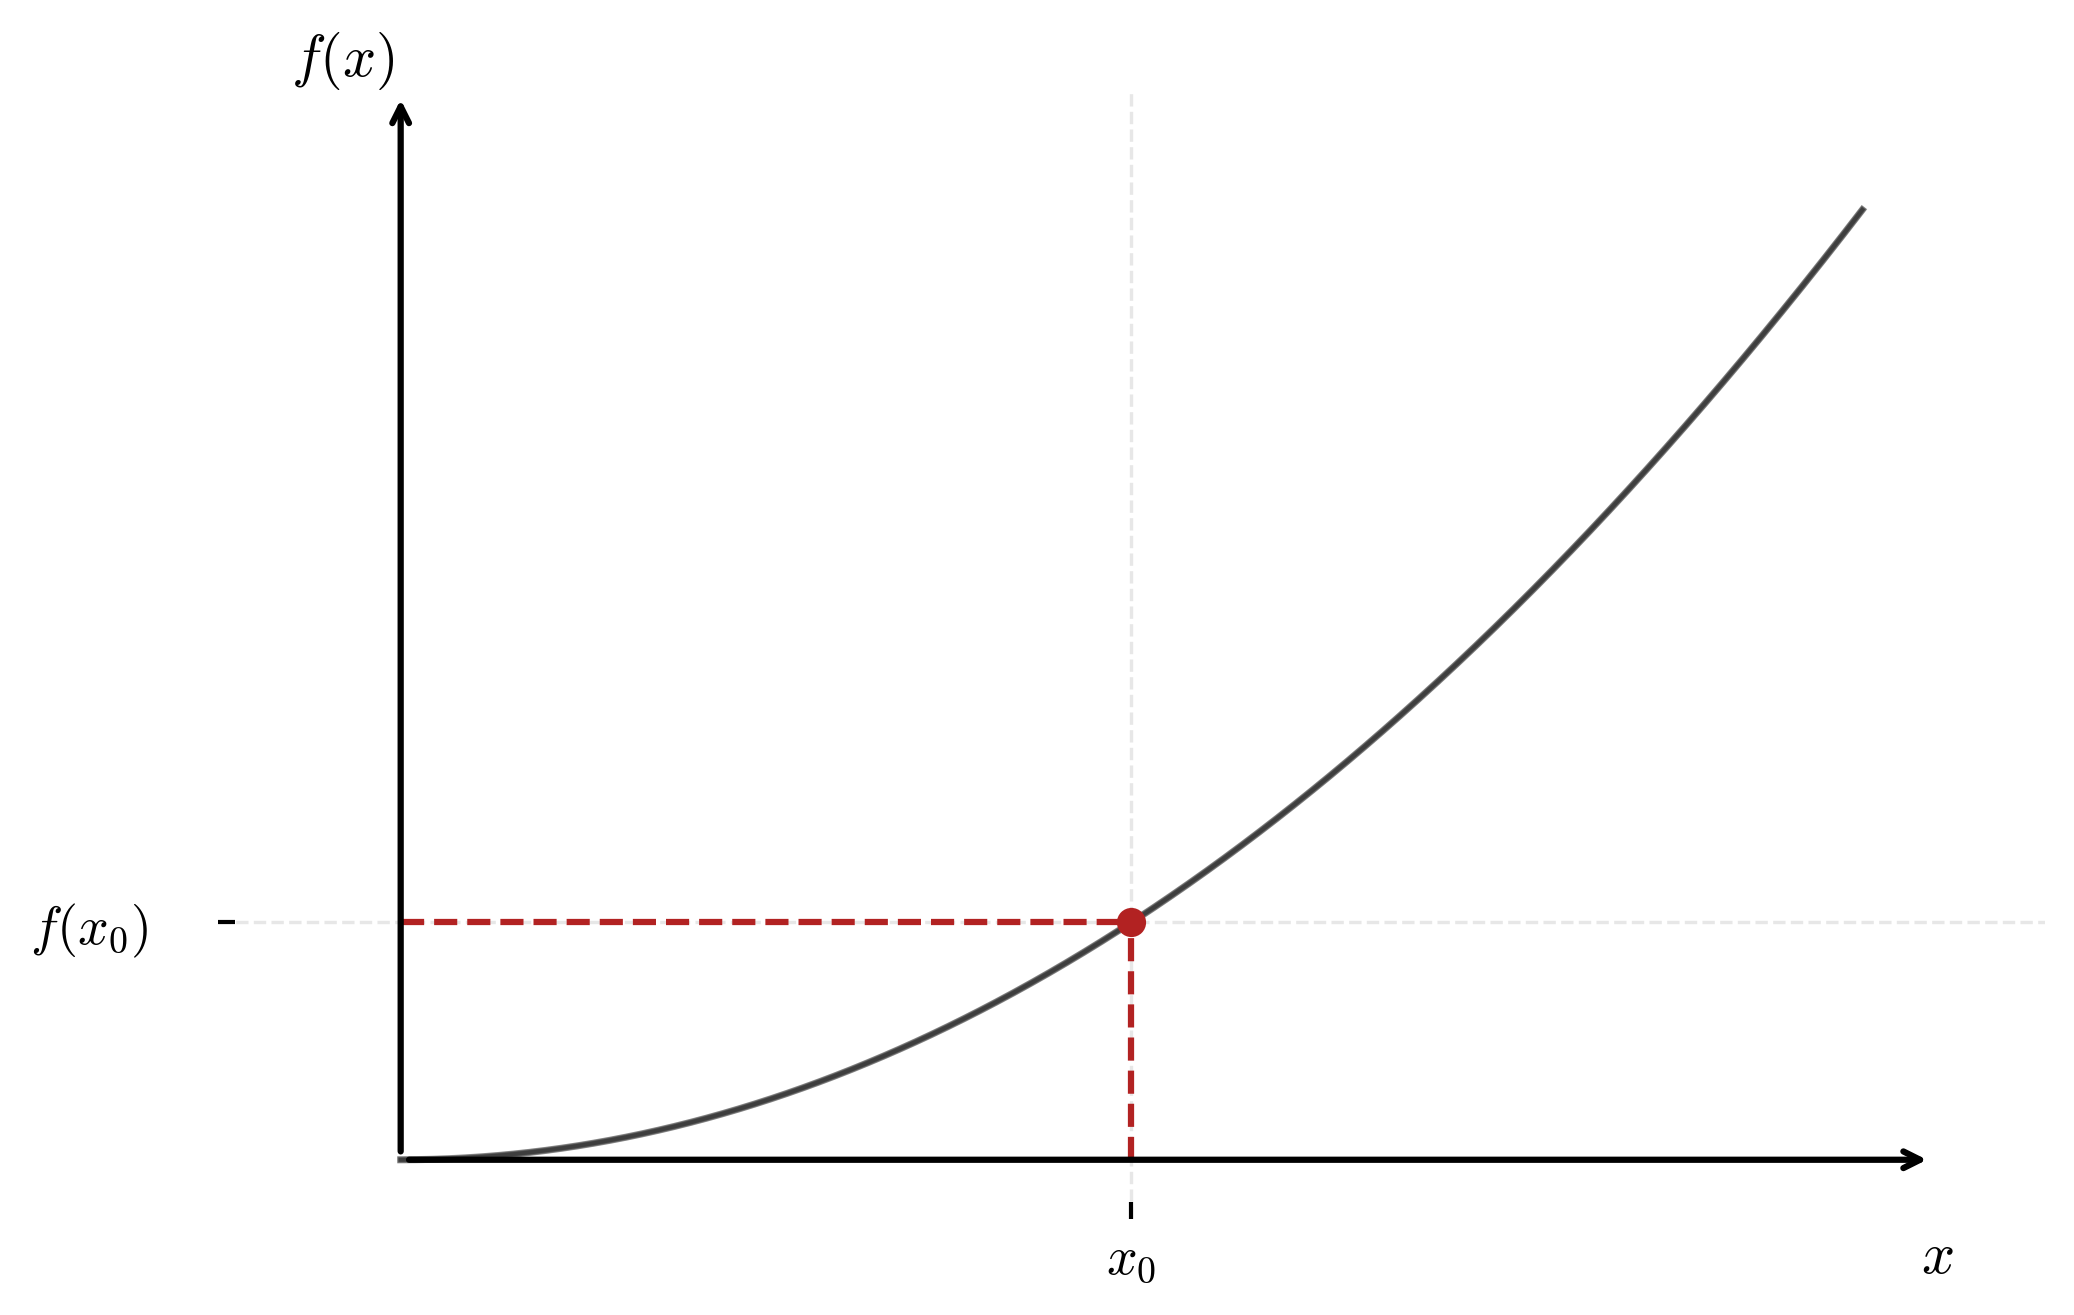
\includegraphics[width=0.7\textwidth]{figures/appendix/functions_point_1.png}
    \caption{Representation of a function $f(x)$, a given point $x_0$ and its image $f(x_0)$.}
    \label{fig:functions_point_1}
\end{figure}

The seeds of calculus began to germinate more concretely in the late medieval and early Renaissance periods. The Indian mathematician Bhāskara II (12th century) hinted at the idea of instantaneous rates of change, and later, the French philosopher René Descartes (1596--1650) and the English mathematician John Wallis (1616--1703) laid important groundwork in algebra and infinite series. But calculus, as a coherent system, was born in the late 17th century through the independent and nearly simultaneous efforts of \textbf{Isaac Newton} (1643--1727) in England and \textbf{Gottfried Wilhelm Leibniz} (1646--1716) in Germany. Newton, motivated by problems in physics---such as planetary motion and gravitation---developed what he called ``the method of fluxions,'' focusing on rates of change and motion. Leibniz, meanwhile, introduced a notational system and conceptual clarity that would become the foundation for the modern symbolic language of calculus. His elegant integral sign $\int$ and differential notation $dx$, $dy$ remain standard to this day.\\

\section{Change, slope and minima: derivatives}

Once we are familiar with the idea of functions as a way of representing the relation between two variables, we can try to model how functions \textit{change}. As already mentioned, this builds upon the work of Newton and Leibniz, although the actual mathematical language we will use was developed much later. Consider we have a function $f(x)$, like the one represented in the figure below. Regardless of the specific shape, or dependency, of $f(x)$ we could pick a point $x_0$, and move a small amount $\Delta x$ along the $x$ axis, to $x_0 + \Delta x$. At this point, we could compute how much that change impacts the $y$ axis, just by evaluating $f(x_0)$, and after the displacement $f(x_0 + \Delta x)$

\begin{figure}[ht]
    \centering
    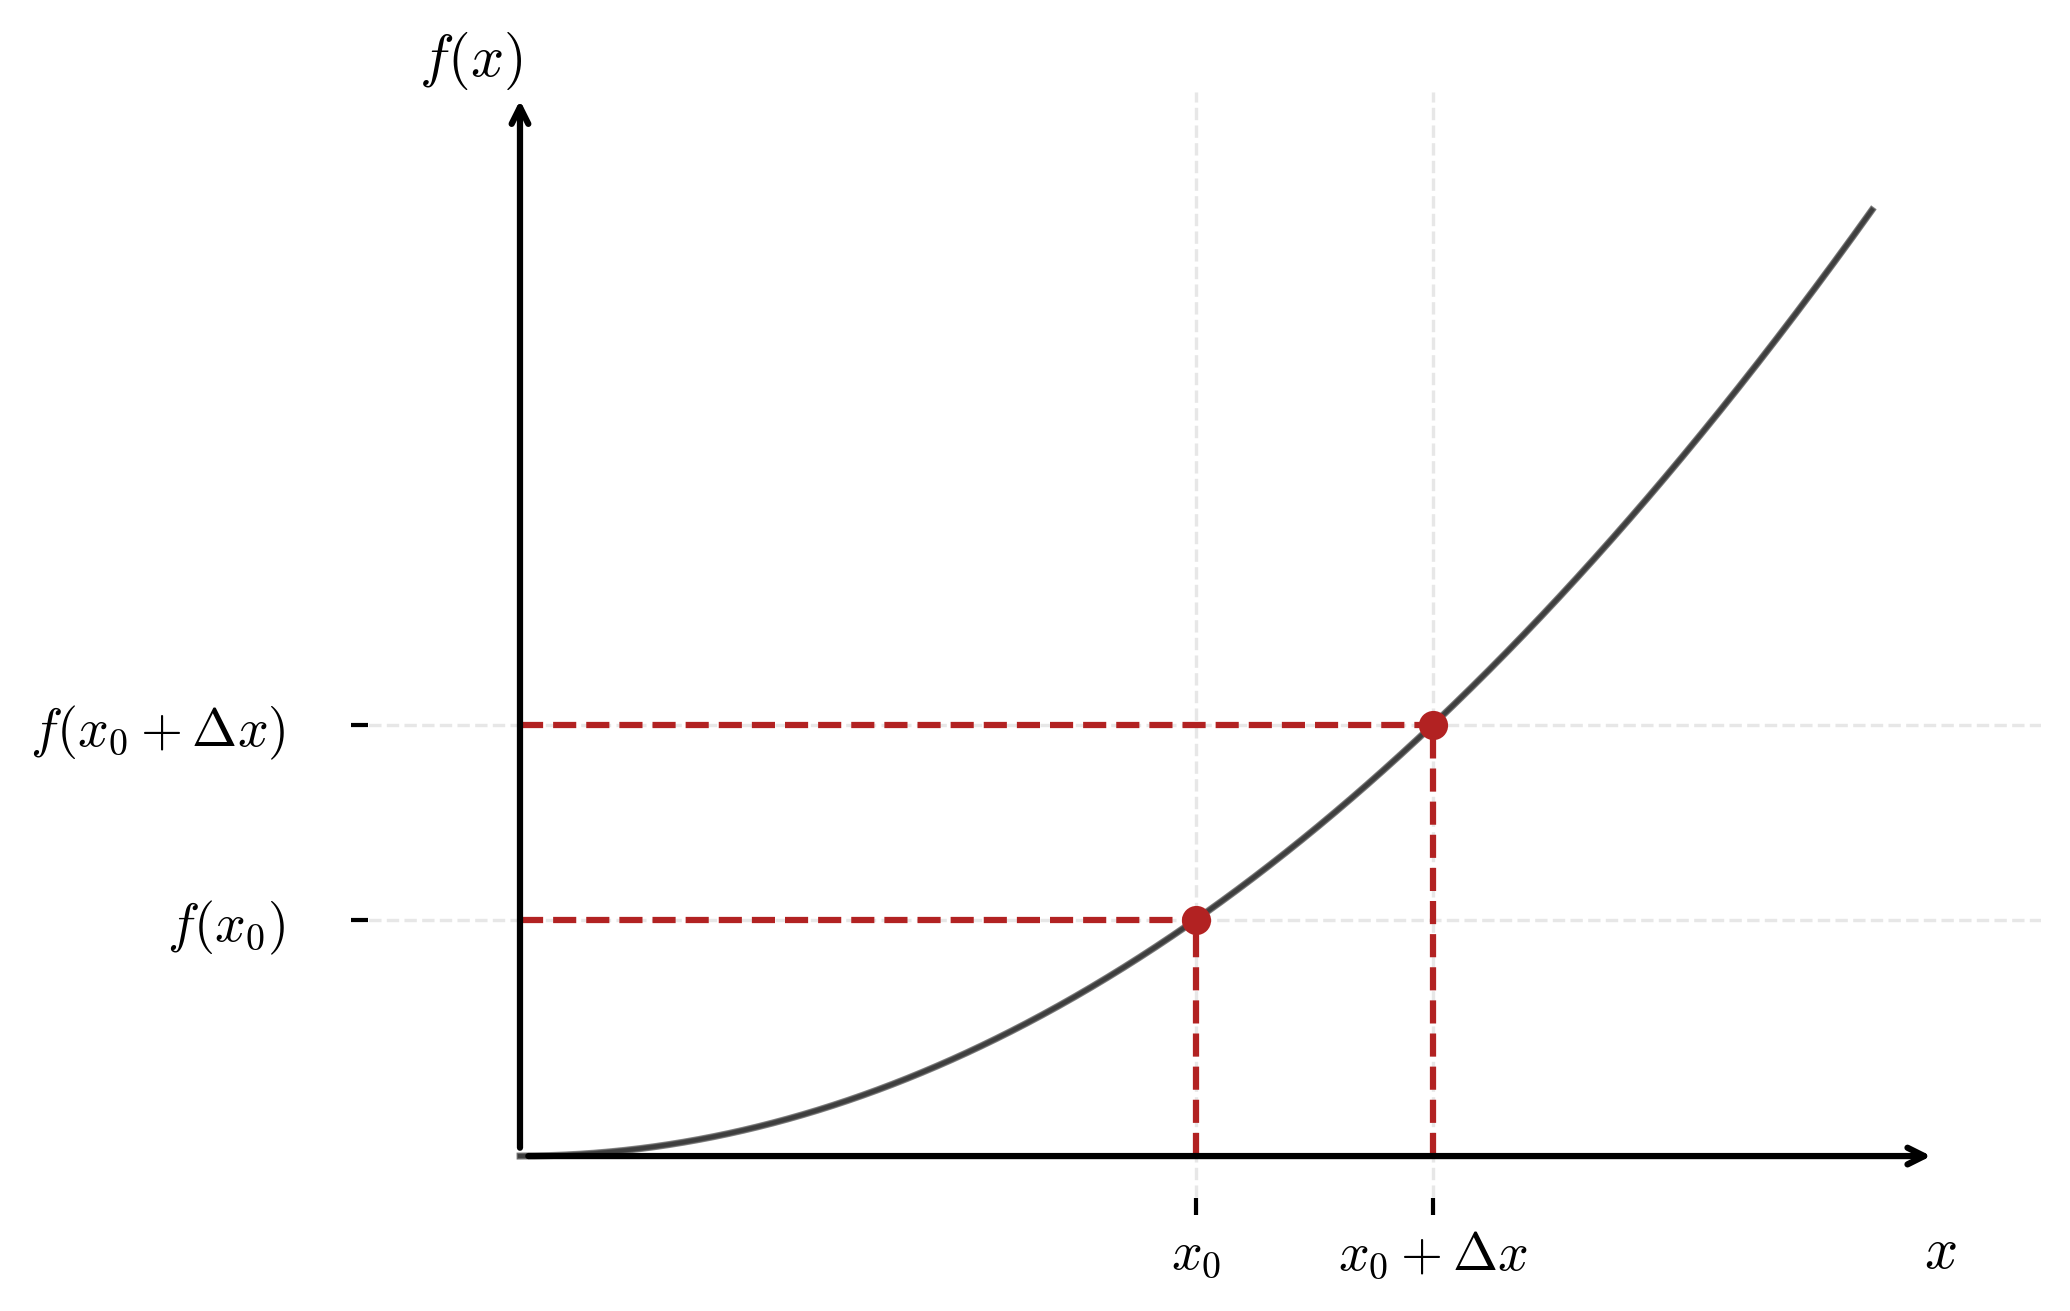
\includegraphics[width=0.7\textwidth]{figures/appendix/functions_point_2.png}
    \caption{Representation of a function $f(x)$, a given point $x_0$ and its image $f(x_0)$, and an increment $\Delta x$ from $x_0$ to $x_0 + \Delta x$. The ratio between the increments in the horizontal axis, $\Delta x$, and the vertical axis $f(x_0 + \Delta x) - f(x_0)$ represents the derivative of the function at that point, that we denote by $f'(x_0)$.}
    \label{fig:functions_point_2}
\end{figure}

To evaluate how fast a function grows - or decreases, to capturing the idea of \emph{change}, we could just compute the ratio if the difference $\Delta x$, and the corresponding change in $f(x)$, 
\begin{equation}
	\frac{f(x + \Delta x) - f(x)}{\Delta x} \quad.
\end{equation}

The derivative of \( f \) at a point \( x_0 \) is defined just as that ratio, for an infinitesimally small $\Delta x$:
\begin{equation}
	f'(x) = \lim_{\Delta x \to 0} \frac{f(x + \Delta x) - f(x)}{\Delta x}
\end{equation}

This expression represents the slope of the tangent line to \( f(x) \) at the point \( x_0 \). If the limit exists, \( f \) is said to be \emph{differentiable} at \( x \). It measures how a function responds to small variations in its input. Intuitively, if a function \( f(x) \) describes a quantity, then its derivative \( f'(x) \) tells us how fast that quantity is changing at each point. There are several notations for the derivative, listed as follows:
\[
f'(x), \quad \frac{df}{dx}, \quad \frac{dy}{dx} \quad \text{(if } y = f(x) \text{)}
\]
Each emphasizes a slightly different aspect. The first notation, attributed to Newton, represents $f'(x)$ as a function, while Leibniz notation $df / dx$, express it as a rate of change, the ratio of increments along the function $\Delta f$ over $\Delta x$. Notations may change across books and literature sources; here we will denote $\Delta$ an increment of arbitrary size, and we will call it \textit{infinitesimal}, or \textit{differential}, when we write it as $dx$

\begin{figure}[ht]
    \centering
    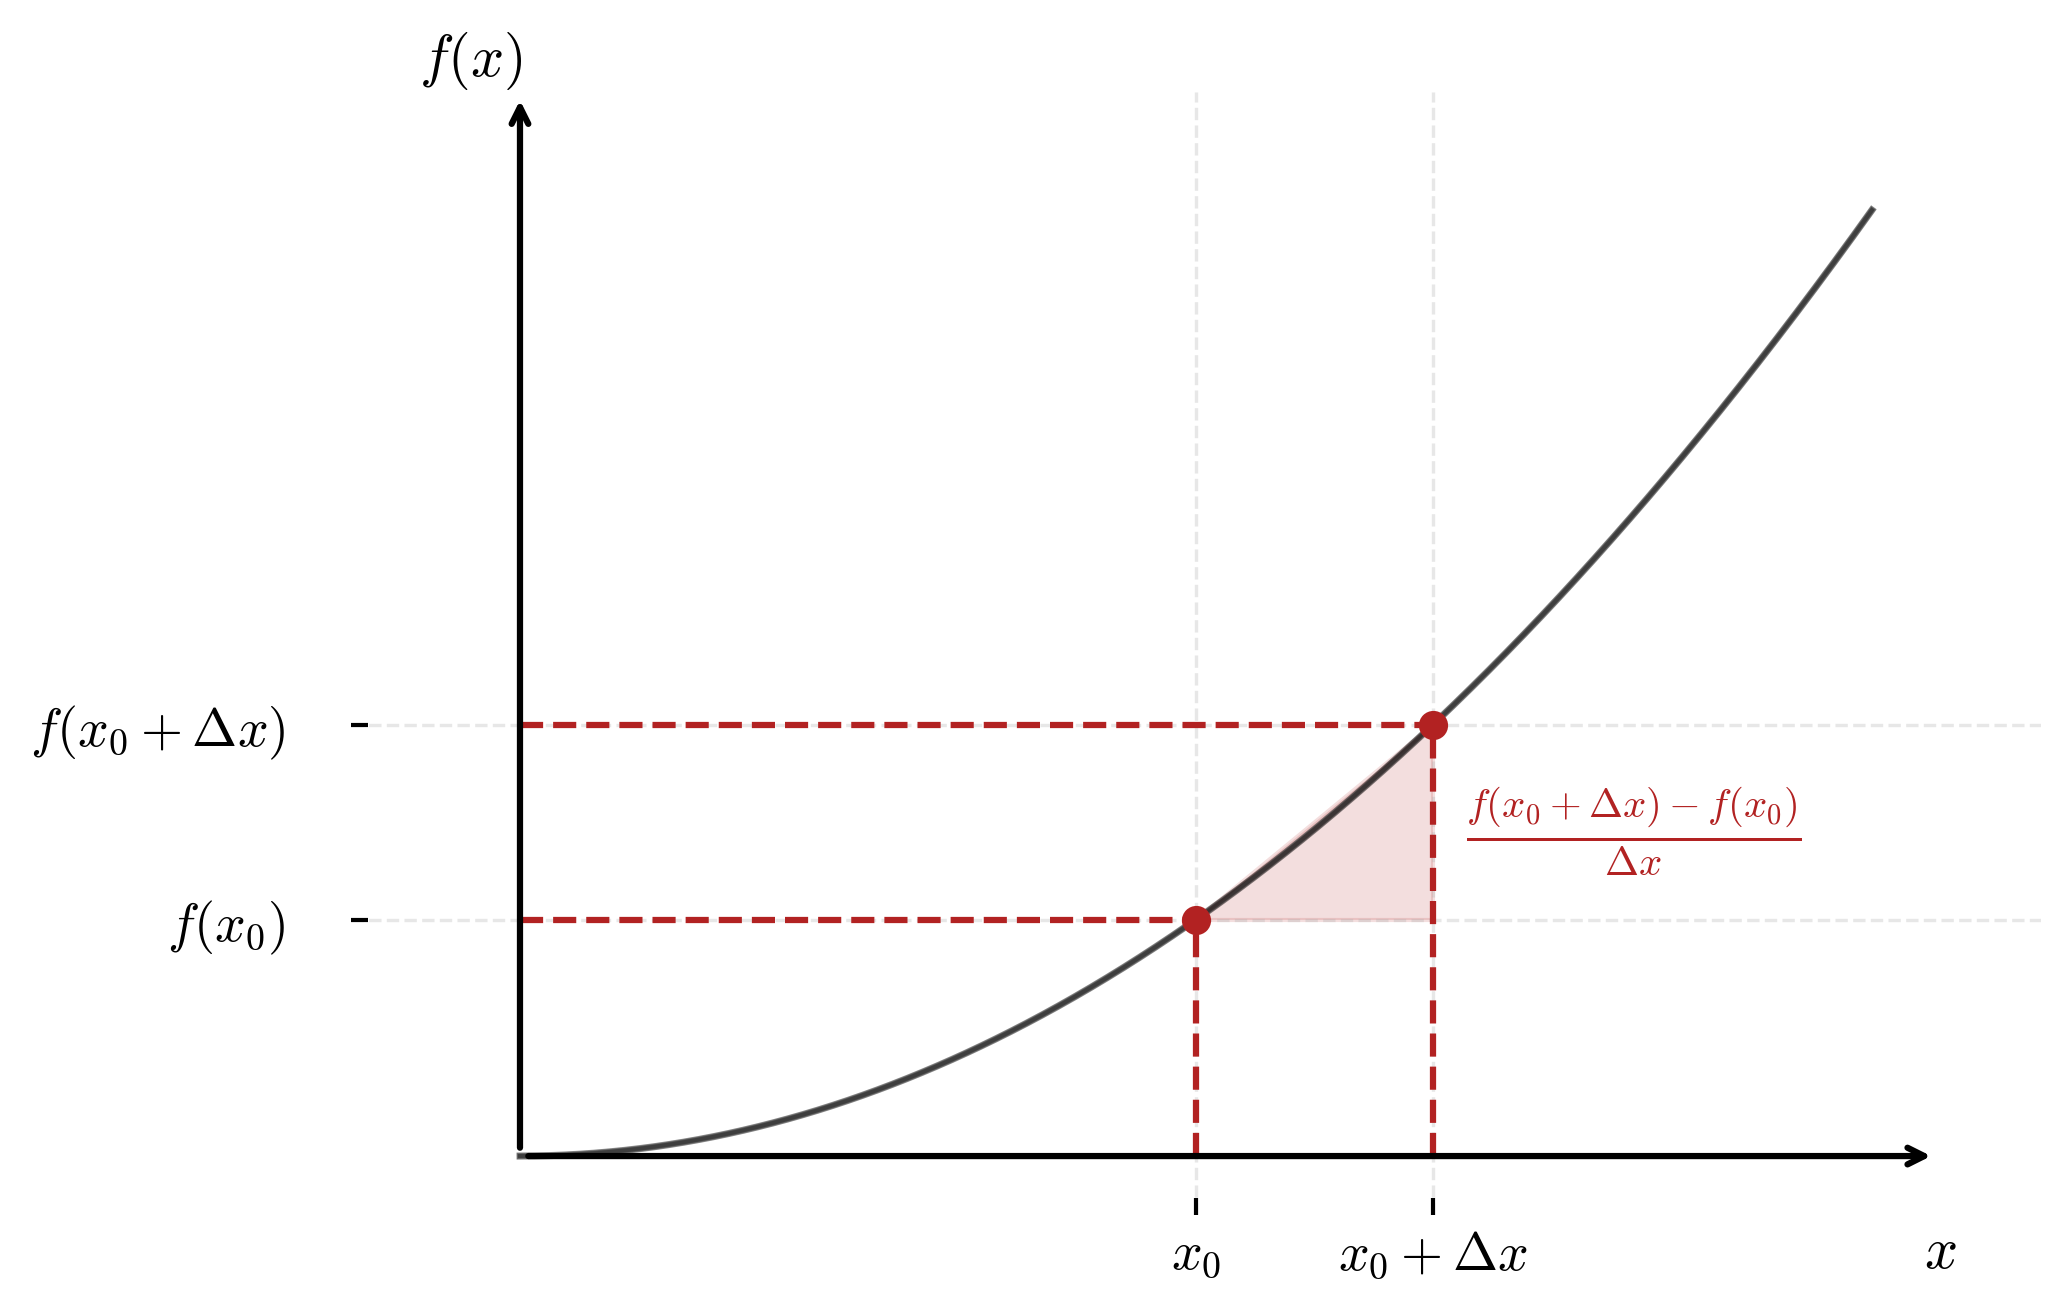
\includegraphics[width=0.7\textwidth]{figures/appendix/functions_point_2_shadow.png}
    \caption{Representation of a function $f(x)$, a given point $x_0$ and its image $f(x_0)$, and an increment $\Delta x$ from $x_0$ to $x_0 + \Delta x$. The ratio between the increments in the horizontal axis, $\Delta x$, and the vertical axis $f(x_0 + \Delta x) - f(x_0)$ represents the derivative of the function at that point, that we denote by $f'(x_0)$.}
    \label{fig:functions_point_2_shadow}
\end{figure}

Hence, we can characterize the equilibrium - or \textit{stationary} - points of a function, its maxima and minima, just by the condition

\begin{equation}
	f'(x) = 0 \quad .
\end{equation}

Wherever a change along $x$ does not affect $f(x)$, meaning $f(x_0 + \Delta x) - f(x_0) = 0$, will be either a maximum or a minimum, and we know that there is no growth around that point $x_0$.\\

The development of calculus marked a turning point in intellectual history. It gave scientists, engineers, and economists the tools to model the world with precision and predict its behavior with confidence. The mathematical machinery behind electricity, fluid dynamics, statistics, and quantum mechanics all rely on the principles laid down by Newton, Leibniz, Euler, and their successors. Yet beyond its utility, calculus offers something more enduring: a glimpse into the deep continuity that underlies the universe, where motion and form, quantity and change, are all expressions of a single, evolving logic. Through calculus and the language of functions, we do not merely calculate---we begin to understand.\\

Geometrically, the derivative represents the slope of the tangent line to the curve \( y = f(x) \). Physically, if \( f(t) \) describes the position of a moving object as a function of time, then \( f'(t) \) gives its instantaneous velocity.

\subsection*{Example}

If \( f(x) = x^2 \), then:
\[
f'(x) = \lim_{\Delta x \to 0} \frac{(x + \Delta x)^2 - x^2}{\Delta x}
= \lim_{\Delta x \to 0} \frac{2x\Delta x + (\Delta x)^2}{\Delta x}
= 2x
\]

Thus, the derivative of \( x^2 \) is \( 2x \), meaning the rate of change increases linearly with \( x \).

The development of calculus marked a turning point in intellectual history. It gave scientists, engineers, and economists the tools to model the world with precision and predict its behavior with confidence. The mathematical machinery behind electricity, fluid dynamics, statistics, and quantum mechanics all rely on the principles laid down by Newton, Leibniz, Euler, and their successors. Yet beyond its utility, calculus offers something more enduring: a glimpse into the deep continuity that underlies the universe, where motion and form, quantity and change, are all expressions of a single, evolving logic. Through calculus and the language of functions, we do not merely calculate---we begin to understand.\\

\section{Divergence and gradient: differential calculus}

Divergence and gradient: differential calculus



% Chapter: Integrals
\chapter{Appendix: Integrals: a quick review}

Integral calculus is the mathematics of accumulation and area, of summing infinitesimal parts to understand wholes. Where differential calculus dissects change, integral calculus assembles continuity---weaving together countless small contributions to reveal the total. It addresses fundamental questions: How much space does a shape occupy? How much work is done over a path? How do quantities build up over time? From measuring land in antiquity to solving complex equations in physics, integral calculus has served as a bridge between the discrete and the continuous, the finite and the infinite.\\

The Historical Origins of Integration. The intuitive idea of integration—measuring area under a curve or volume under a surface—dates back to the ancient world. The Greek mathematician \textbf{Eudoxus of Cnidus} (c.~390--337 BCE) developed the \emph{method of exhaustion}, a precursor to integration, which used successively refined polygons to approximate areas and volumes. \textbf{Archimedes} (c.~287--212 BCE), perhaps the greatest of ancient mathematicians, applied this method to derive results such as the area of a parabola segment and the volume of a sphere, anticipating integral calculus by nearly two millennia\\

Yet it was not until the 17th century that integration found its modern form. The crucial turning point came with the realization that integration and differentiation are inverse processes. This insight was crystallized by \textbf{Isaac Newton} (1642--1727) and \textbf{Gottfried Wilhelm Leibniz} (1646--1716), working independently. Newton, motivated by problems in physics, viewed integration as the accumulation of continuous quantities like motion and force. Leibniz, meanwhile, formalized the symbolic language of integration, introducing the elongated $S$ symbol ($\int$) for summation and $dx$ for infinitesimal change. His notational clarity profoundly shaped the development of analysis.\\

Their work established what we now call the \textbf{Fundamental Theorem of Calculus}, which states that integration and differentiation are inverse operations:

\[
\frac{d}{dx} \left( \int_a^x f(t)\, dt \right) = f(x)
\qquad \text{and} \qquad
\int_a^b f'(x)\, dx = f(b) - f(a)
\]

This theorem provided both the conceptual unity and practical tools to solve problems in geometry, physics, and beyond.\\

Rigor and Expansion. Though powerful, early calculus lacked rigor. Questions arose: What precisely is a limit? What functions can be integrated? These were resolved over the 18th and 19th centuries by mathematicians such as \textbf{Augustin-Louis Cauchy} (1789--1857), who formalized limits and continuity, and \textbf{Bernhard Riemann} (1826--1866), who defined integration through Riemann sums, grounding the intuitive notion of area in precise terms. Later, \textbf{Henri Lebesgue} (1875--1941) expanded the theory further with the \emph{Lebesgue integral}, which could handle more pathological functions and laid the foundation for modern measure theory. This broader framework enabled integration in more abstract contexts, from probability spaces to Hilbert spaces, and opened the door to modern analysis and functional integration.\\

\begin{figure}[ht]
    \centering
    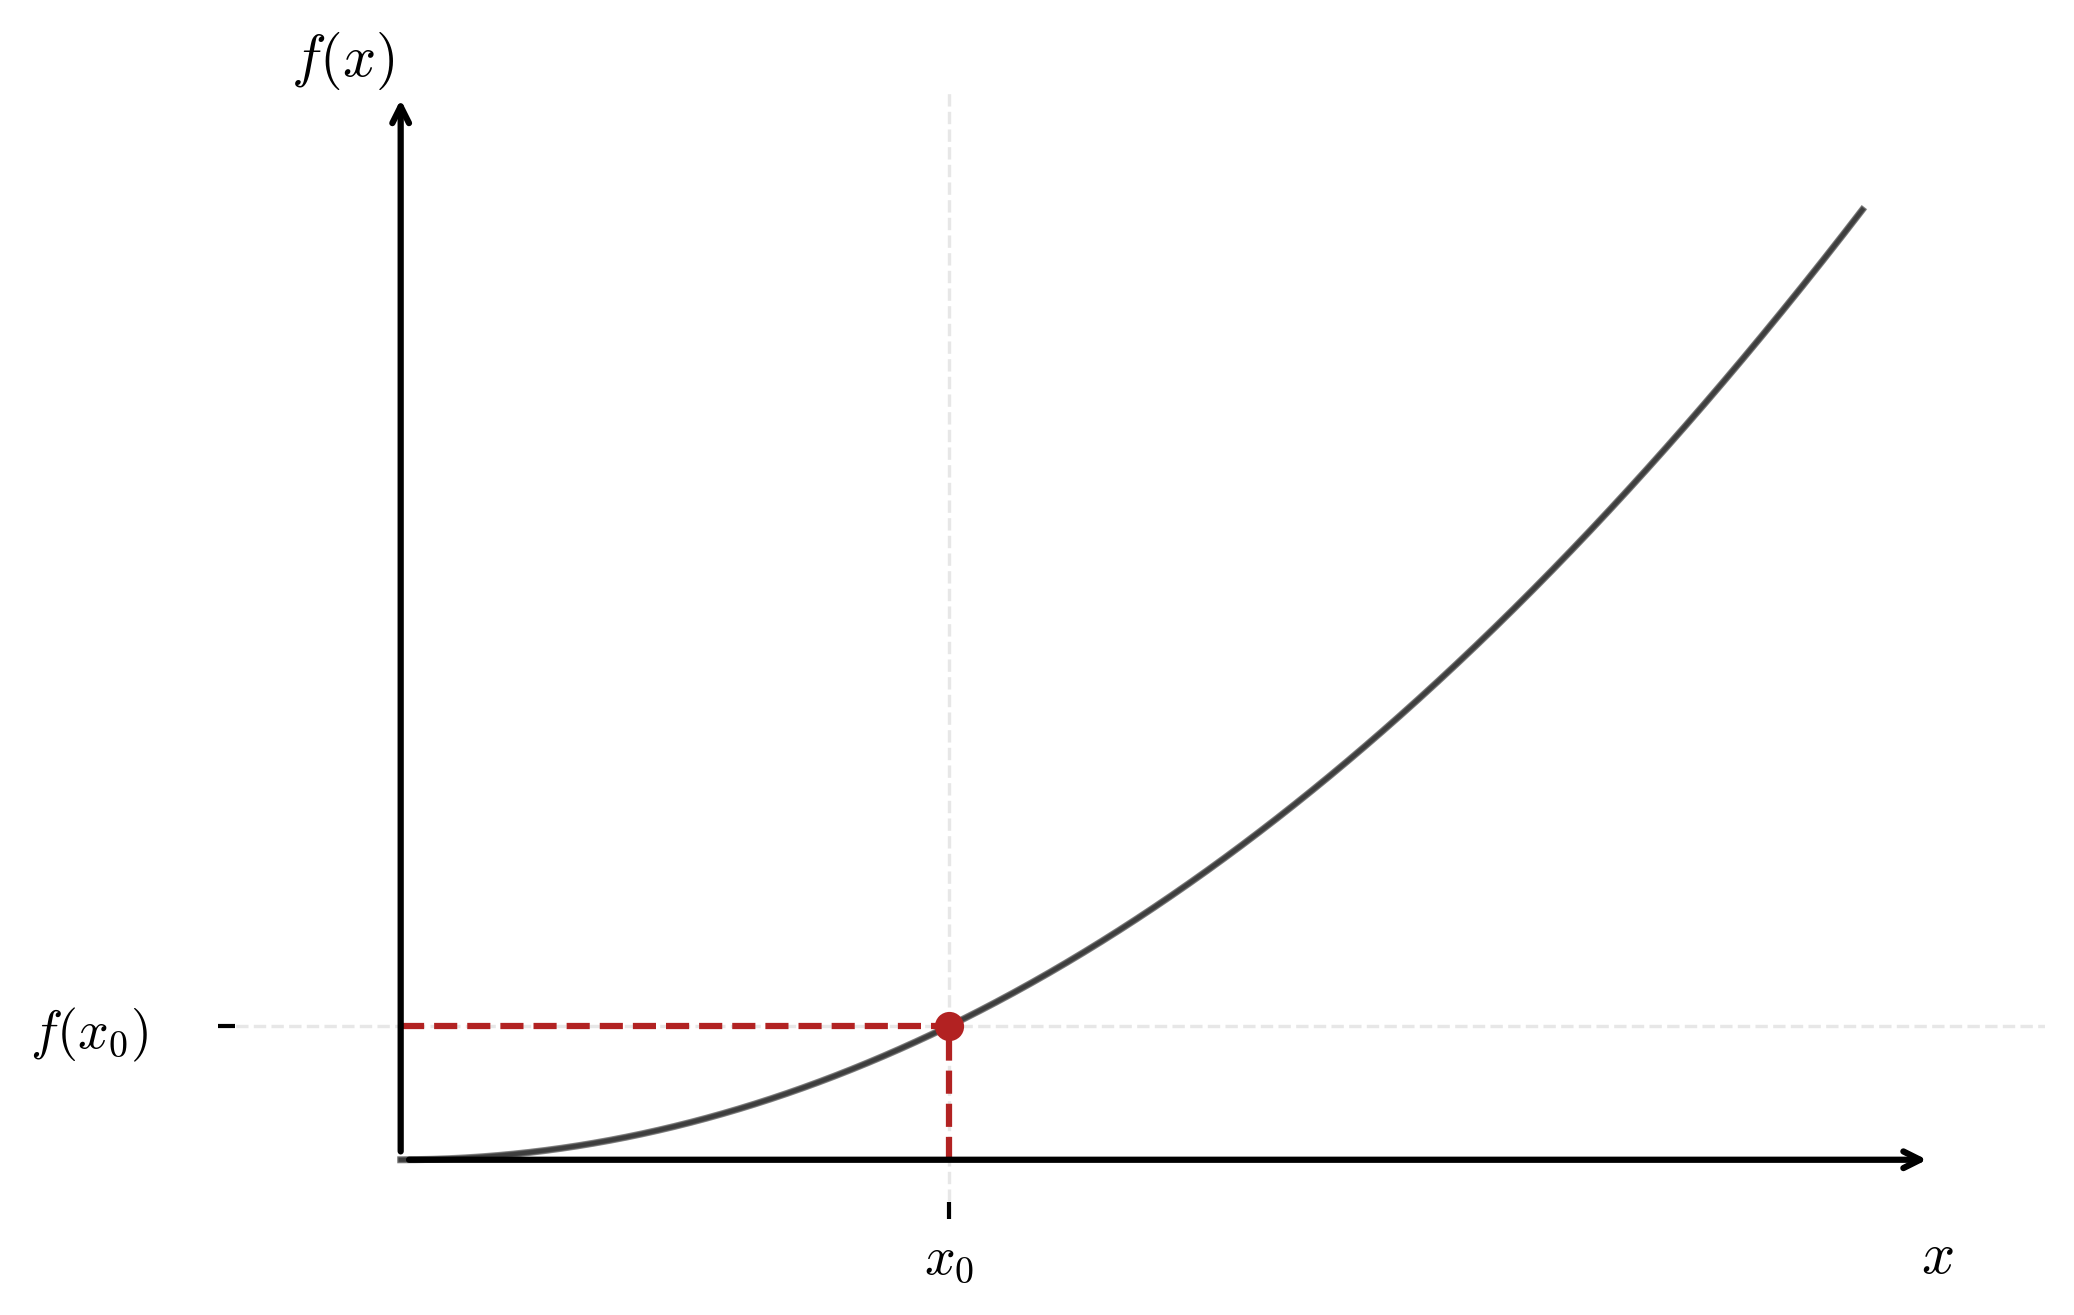
\includegraphics[width=0.7\textwidth]{figures/appendix/integrals_1.png}
    \caption{Representation of a function $f(x)$, a given point $x_0$ and its image $f(x_0)$, and an increment $\Delta x$ from $x_0$ to $x_0 + \Delta x$.}
    \label{fig:integrals_1}
\end{figure}

\begin{figure}[ht]
    \centering
    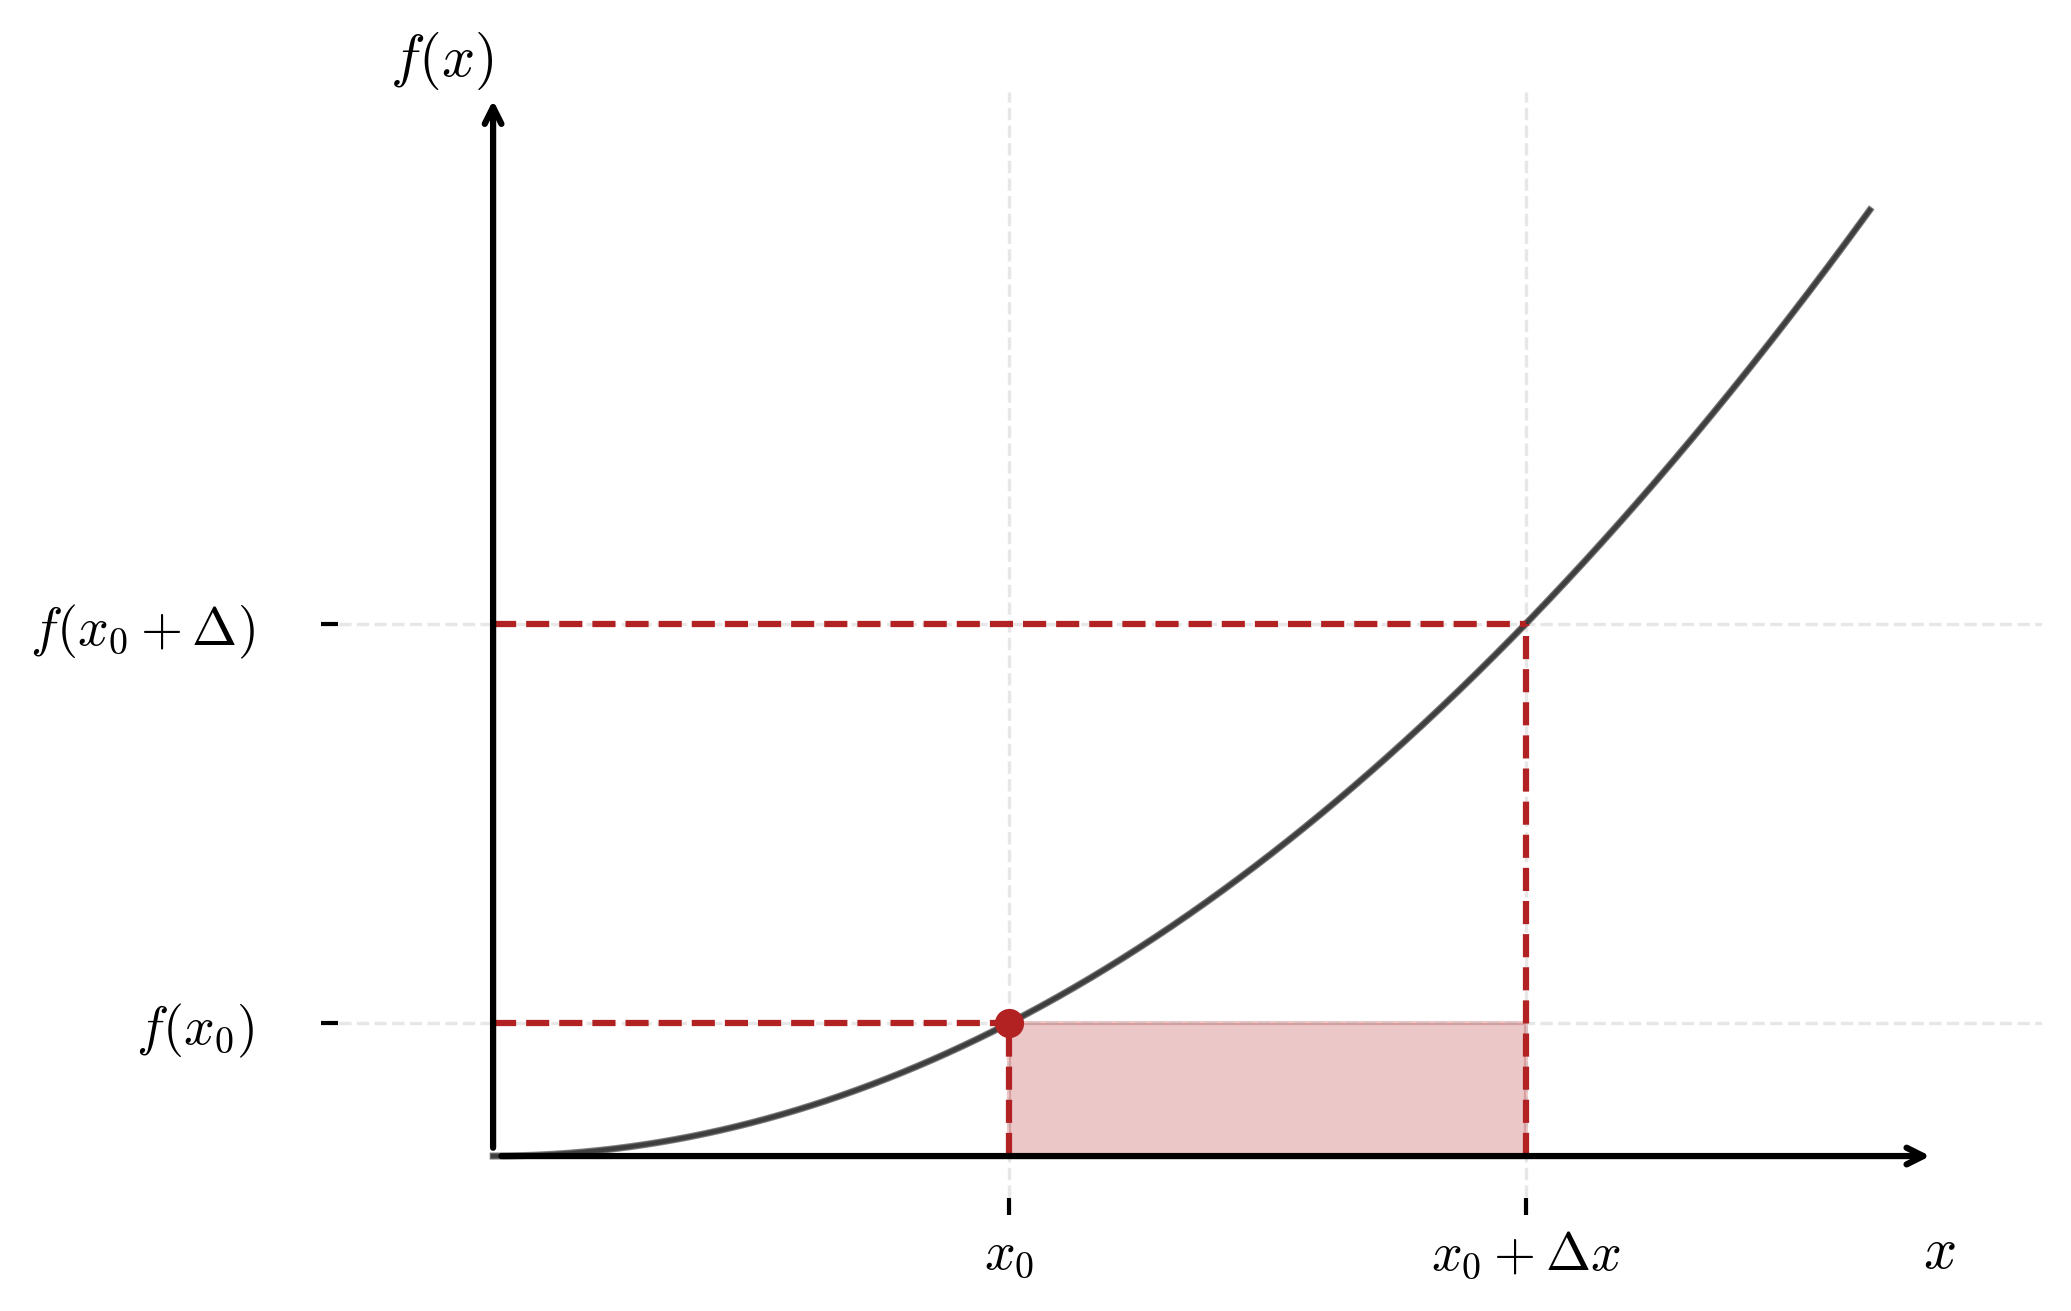
\includegraphics[width=0.7\textwidth]{figures/appendix/integrals_2.png}
    \caption{Representation of a function $f(x)$, a given point $x_0$ and its image $f(x_0)$, and an increment $\Delta x$ from $x_0$ to $x_0 + \Delta x$. Here we divide the $\Delta x$ increment in smaller steps, aiming to approximate the area under the function. As the subdivisions become smaller, they become a better approximation of the area, and in the limit $\Delta x \rightarrow \infty$ they converge to the Riemann definition.}
    \label{fig:integrals_2}
\end{figure}

\begin{figure}[ht]
    \centering
    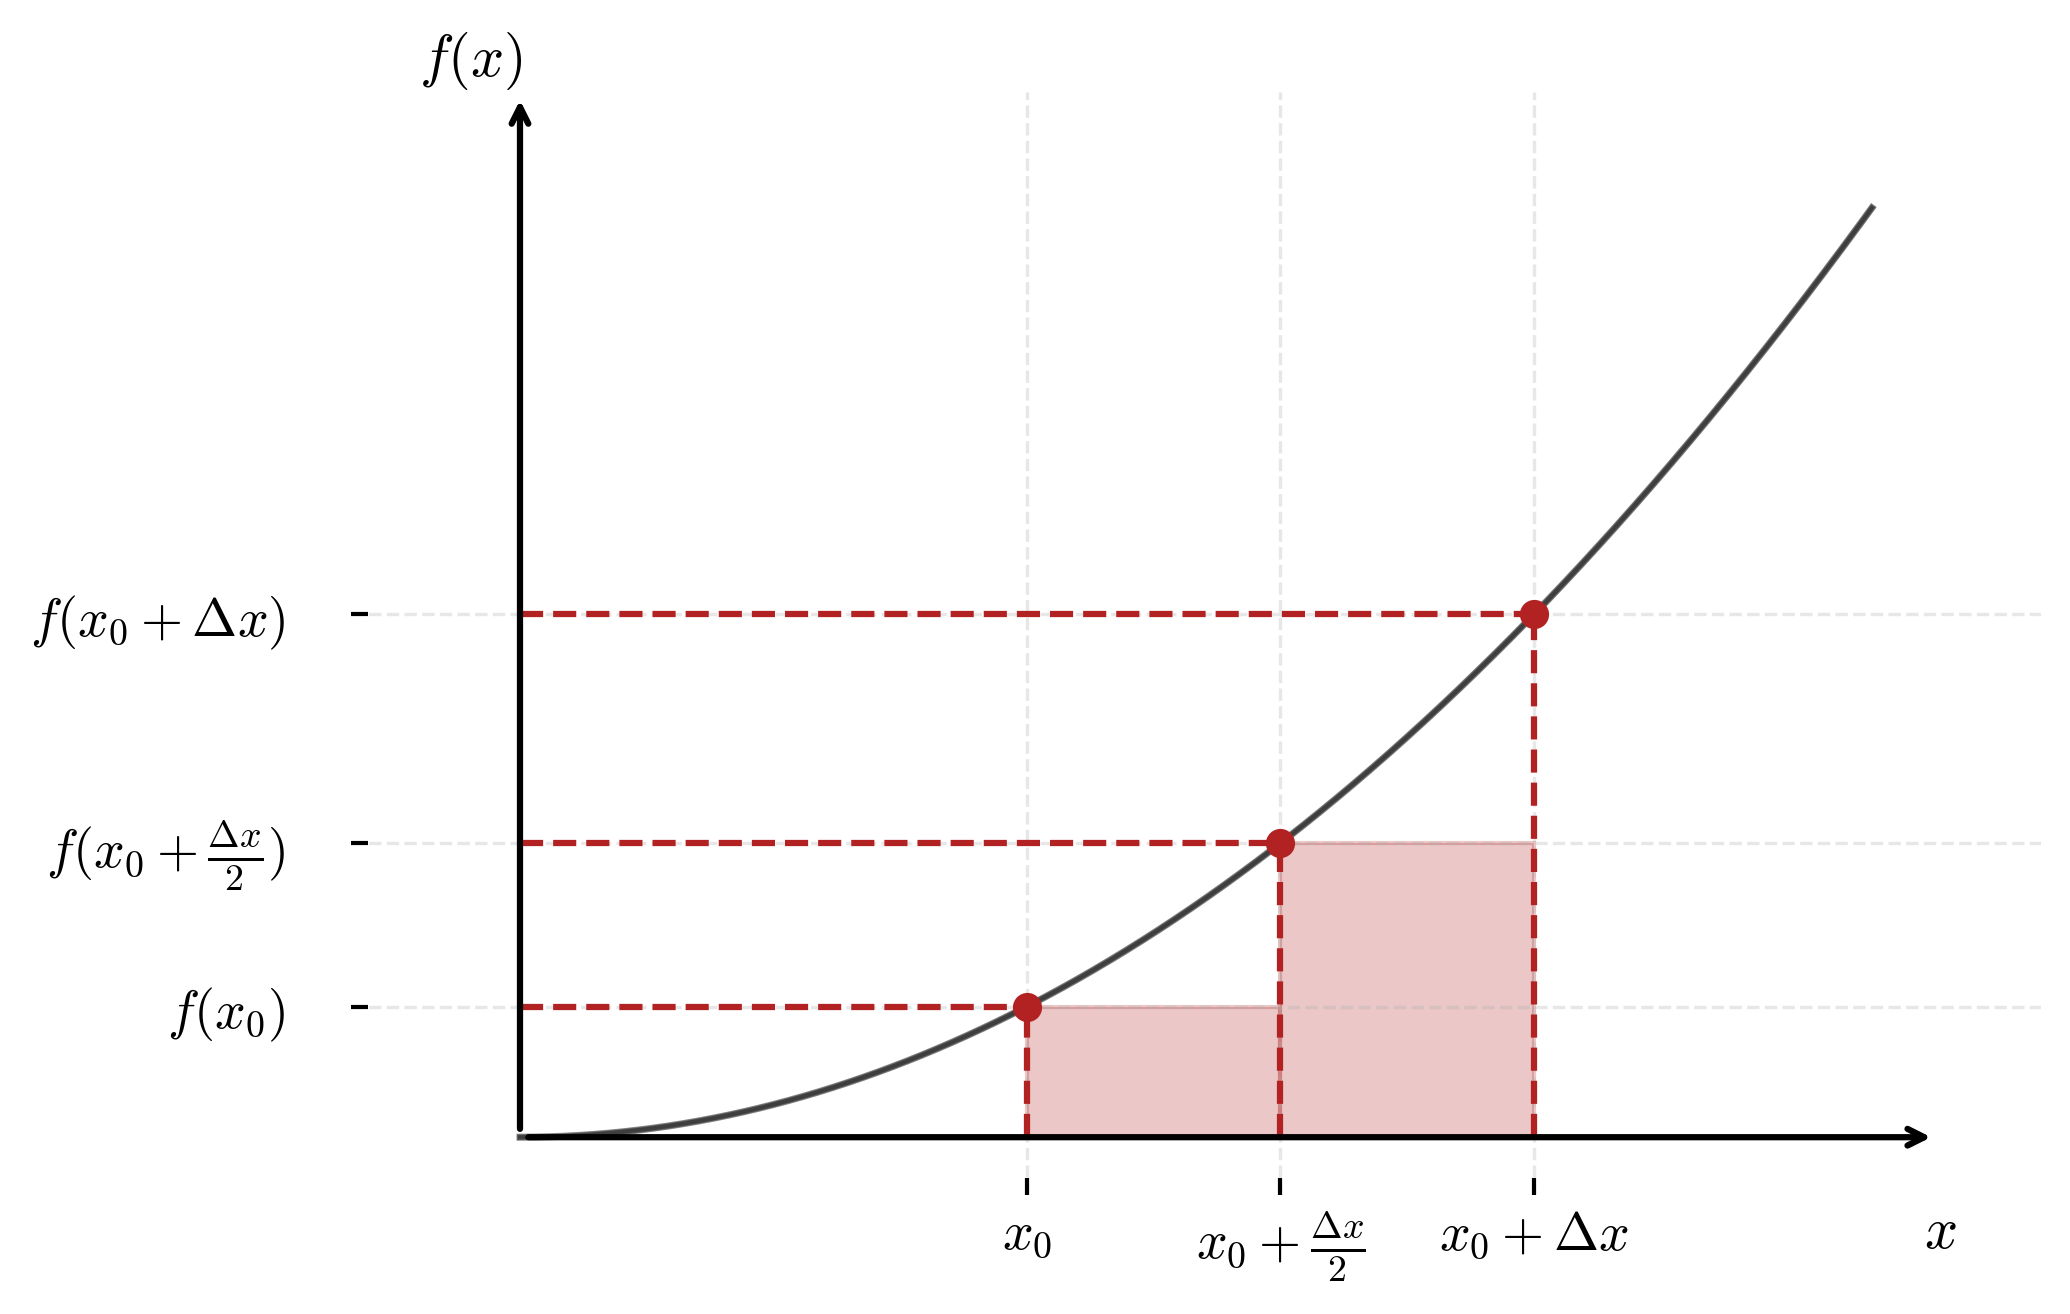
\includegraphics[width=0.7\textwidth]{figures/appendix/integrals_2_subdivisions.png}
    \caption{Representation of a function $f(x)$, a given point $x_0$ and its image $f(x_0)$, and an increment $\Delta x$ from $x_0$ to $x_0 + \Delta x$. Here we divide the $\Delta x$ increment in smaller steps, aiming to approximate the area under the function. As the subdivisions become smaller, they become a better approximation of the area, and in the limit $\Delta x \rightarrow \infty$ they converge to the Riemann definition.}    \label{fig:integrals_2_subdivisions}
\end{figure}

Together, these statements tell us that the process of summing infinitesimal contributions to find total accumulation (integration) and the process of finding the instantaneous rate of change (differentiation) are fundamentally linked. This profound insight lies at the heart of calculus, enabling the solution of countless problems in physics, engineering, and beyond.

\begin{figure}[ht]
    \centering
    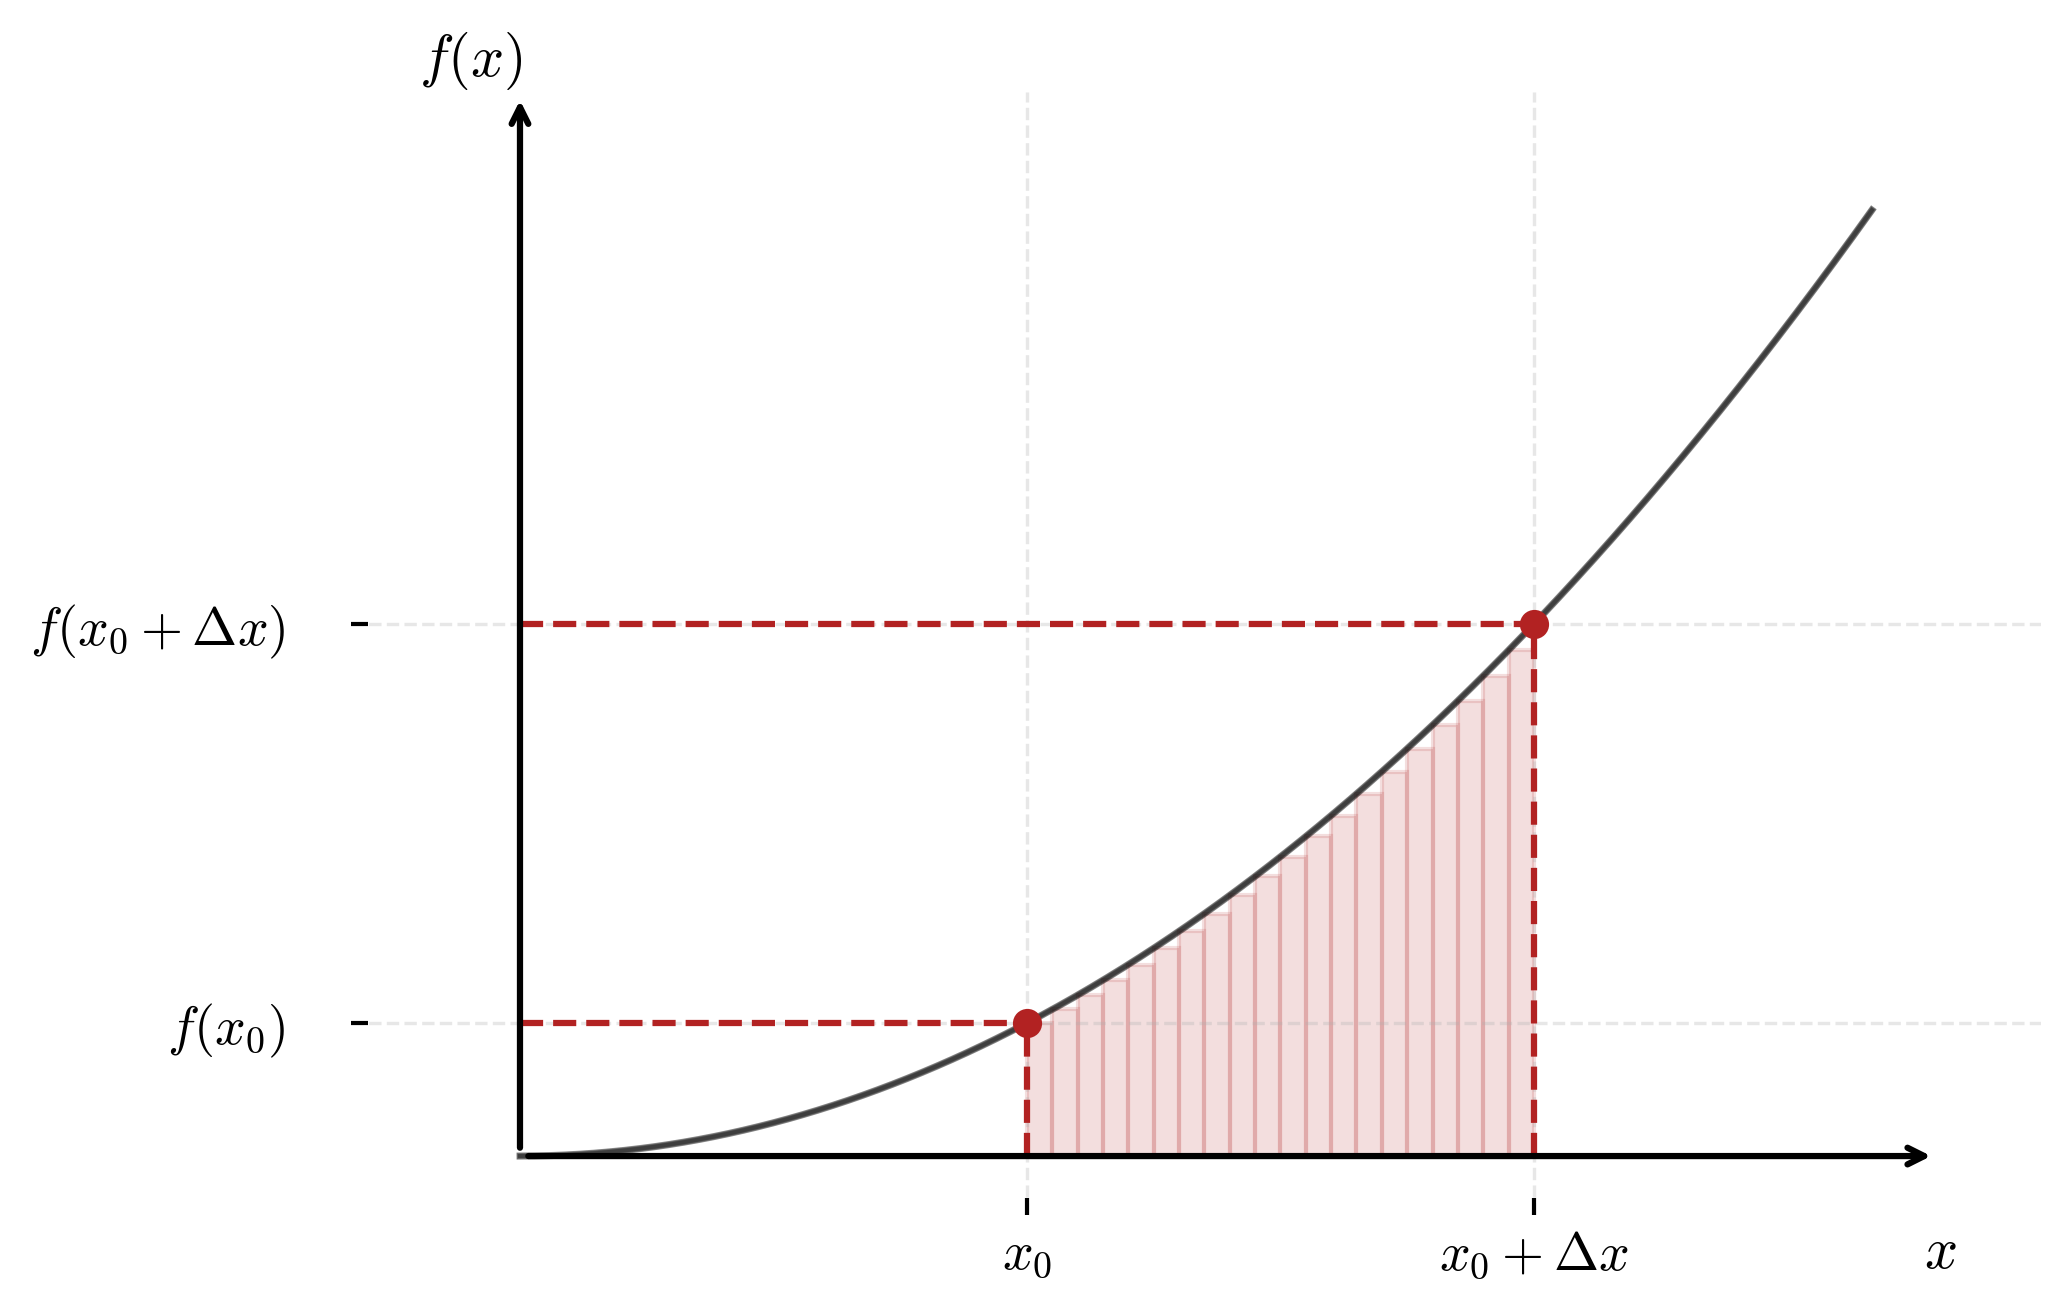
\includegraphics[width=0.7\textwidth]{figures/appendix/integrals_3_riemann.png}
    \caption{Representation of a function $f(x)$, a given point $x_0$ and its image $f(x_0)$, and an increment $\Delta x$ from $x_0$ to $x_0 + \Delta x$. Here we divide the $\Delta x$ increment in smaller steps, aiming to approximate the area under the function. As the subdivisions become smaller, they become a better approximation of the area, and in the limit $\Delta x \rightarrow \infty$ they converge to the Riemann definition.}
    \label{fig:integrals_3_riemann}
\end{figure}

Applications and Legacy.Integral calculus plays a central role in virtually every branch of science and engineering. In physics, it describes the flow of fluids, the propagation of waves, the accumulation of charge, and the work done by forces over time. In economics, it models total cost, revenue, and utility. In biology and medicine, it helps quantify rates of growth, spread of populations, and diffusion processes.\\

Computationally, integration techniques underpin numerical methods, algorithms for simulations, and digital signal processing. In probability theory, integrals define expected values and distributions, while in geometry and topology, integration is used to calculate lengths, areas, and volumes in curved and abstract spaces.\\

The Spirit of Integral Calculus. Integral calculus teaches us to think holistically---to understand how global behavior arises from local contributions. It invites us to see curves not just as paths but as stories of accumulation: of distance traveled, energy stored, substance gathered. From the earliest geometric approximations to the abstract theories of modern analysis, integration has grown into one of the most powerful and beautiful tools in mathematics.\\

To learn integral calculus is to acquire a lens through which we view the continuous world---to perceive not only rates of change, but the subtle ways in which all things are built up from infinitesimal parts. It is a mathematics of synthesis, binding motion to rest, parts to whole, and analysis to intuition.

\section{Indefinite integral as antiderivative}

Integral calculus complements the derivative by focusing on \emph{accumulation} rather than instantaneous change. It allows us to find areas under curves, total quantities accumulated over an interval, and much more.

\subsection*{Definite Integral}

Given a function \( f(x) \) defined on an interval \([a, b]\), the definite integral of \( f \) from \( a \) to \( b \) is intuitively the total accumulation of the values of \( f \) over that interval. It is formally defined as the limit of Riemann sums:

\[
\int_a^b f(x) \, dx = \lim_{n \to \infty} \sum_{i=1}^n f(x_i^*) \, \Delta x_i
\]

where the interval \([a, b]\) is partitioned into subintervals of length \(\Delta x_i\), and \(x_i^*\) is a sample point in the \(i\)-th subinterval. This sum approximates the area under the curve \( y = f(x) \) between \( x = a \) and \( x = b \).

The Fundamental Theorem of Calculus bridges differentiation and integration, showing they are inverse processes. It has two parts:

\begin{itemize}
    \item \textbf{Part 1:} If \( F(x) \) is defined by
    \[
    F(x) = \int_a^x f(t) \, dt,
    \]
    where \( f \) is continuous on \([a,b]\), then \( F \) is differentiable and
    \[
    F'(x) = f(x).
    \]
    In other words, differentiation “undoes” integration.

    \item \textbf{Part 2:} If \( F \) is any antiderivative of \( f \) on \([a,b]\) (i.e., \( F'(x) = f(x) \)), then
    \[
    \int_a^b f(x) \, dx = F(b) - F(a).
    \]
    This means the definite integral can be evaluated by finding any antiderivative of \( f \).
\end{itemize}

\section{Define definite integral as area under a curve}

Define definite integral as area under a curve

\section{The fundamental theorem of calculus}

The fundamental theorem of calculus



% Bibliography .........................................................................................................................................................
\backmatter
 
\begin{thebibliography}{999}

\bibitem{ioannidis2005why}
John P. A. Ioannidis.
\textit{Why Most Published Research Findings Are False}.
PLoS Medicine, 2(8):e124, 2005.

\bibitem{spiegelhalter2019art} 
David Spiegelhalter. 
\textit{The Art of Statistics: How to Learn from Data}. 
Basic Books, 2019.

\bibitem{degroot2012probability}
Morris H. DeGroot and Mark J. Schervish.
\textit{Probability and Statistics} (4th ed.).
Pearson, 2012.

\bibitem{bandyopadhyay2011philosophy}
P.S. Bandyopadhyay and M.R. Forster (Eds.).
\textit{Philosophy of Statistics}.
Handbook of the Philosophy of Science, Vol. 7, Elsevier, 2011.

\bibitem{openintro2025}
M. Diez, D. Barr, and Çetinkaya-Rundel.
\textit{OpenIntro Statistics}.
OpenIntro, 2025.

\bibitem{pishronik2014introduction}
Hossein Pishro-Nik.
\textit{Introduction to Probability, Statistics and Random Processes}.
Kappa Research LLC, 2014.

\bibitem{finkel2007ancient}
Irving L. Finkel.  
\textit{Ancient Board Games in Perspective}.  
British Museum Press, 2007.

\bibitem{david1962games}
Florence N. David.  
\textit{Games, Gods and Gambling: A History of Probability and Statistical Ideas}.  
Charles Griffin \& Company, 1962.

\bibitem{cicero45bce}
Marcus Tullius Cicero.  
\textit{De Natura Deorum \& De Divinatione}.  
Loeb Classical Library (various editions), ca. 45 BCE.

\bibitem{cardano1663ludo}
Gerolamo Cardano.  
\textit{Liber de Ludo Aleae (Book on Games of Chance)}.  
Posthumously published 1663; English translation in Oystein Ore, \textit{Cardano, The Gambling Scholar}, Princeton University Press, 1953.

\bibitem{devlin2008unfinished}
Keith Devlin.  
\textit{The Unfinished Game: Pascal, Fermat, and the Seventeenth-Century Letter That Made the World Modern}.  
Basic Books, 2008.

\bibitem{huygens1657ratiociniis}
Christiaan Huygens.  
\textit{De Ratiociniis in Ludo Aleae}.  
Published in Latin, 1657.

\bibitem{bernoulli1713ars}
Jacob Bernoulli.  
\textit{Ars Conjectandi}.  
Thurnisius, 1713. English translation by Edith Dudley Sylla, Johns Hopkins University Press, 2006.

\bibitem{hald1990history}
Anders Hald.  
\textit{A History of Probability and Statistics and Their Applications before 1750}.  
Wiley, 1990.

\bibitem{kolmogorov1933grundbegriffe}
Andrey N. Kolmogorov.  
\textit{Grundbegriffe der Wahrscheinlichkeitsrechnung}.  
Springer, 1933. English translation: \textit{Foundations of the Theory of Probability}, Chelsea Publishing Company, 1956.

\bibitem{kolmogorov1933}
A. N. Kolmogorov, \emph{Grundbegriffe der Wahrscheinlichkeitsrechnung}, Springer, 1933.

\bibitem{lebesgue1902}
H. Lebesgue, \emph{Intégrale, longueur, aire}, Annali di Matematica, 1902.

\bibitem{doob1953}
J. L. Doob, \emph{Stochastic Processes}, Wiley, 1953.

\bibitem{vonmises1928}
R. von Mises, \emph{Probability, Statistics and Truth}, 1928.

\bibitem{bayes1763}
T. Bayes, \emph{An Essay towards Solving a Problem in the Doctrine of Chances}, Philosophical Transactions of the Royal Society of London, 1763.

\bibitem{laplace1812}
P.-S. Laplace, \emph{Théorie Analytique des Probabilités}, 1812.

\bibitem{definetti1974}
B. de Finetti, \emph{Theory of Probability}, Wiley, 1974.

\bibitem{billingsley1995}
P. Billingsley, \emph{Probability and Measure}, Wiley, 1995.

\bibitem{jaynes2003}
E. T. Jaynes, \emph{Probability Theory: The Logic of Science}, Cambridge University Press, 2003.

\bibitem{student1908}
Student. (1908). *The probable error of a mean*. Biometrika, 6(1), 1–25.

\bibitem{fisher1925}
Fisher, R. A. (1925). *Statistical Methods for Research Workers*. Edinburgh: Oliver and Boyd.

\bibitem{fisher1935}
Fisher, R. A. (1935). *The Design of Experiments*. Edinburgh: Oliver and Boyd.

\bibitem{pearson1900}
Pearson, K. (1900). *On the criterion that a given system of deviations from the probable in the case of a correlated system of variables is such that it can be reasonably supposed to have arisen from random sampling*. Philosophical Magazine Series 5, 50(302), 157–175.

\bibitem{welch1947}
Welch, B. L. (1947). *The generalization of "Student’s" problem when several different population variances are involved*. Biometrika, 34(1–2), 28–35.

\bibitem{yates1934}
Yates, F. (1934). *Contingency tables involving small numbers and the $\chi^2$ test*. Supplement to the Journal of the Royal Statistical Society, 1(2), 217–235.

\bibitem{greenwood1911}
Greenwood, M., \& Yule, G. U. (1911). *An inquiry into the nature of frequency distributions representative of multiple happenings with particular reference to the occurrence of multiple attacks of disease or of repeated accidents*. Journal of the Royal Statistical Society, 83(2), 255–279.

\end{thebibliography}

\end{document}
